\documentclass[10pt,letterpaper,final]{article}
\usepackage[utf8]{inputenc}
\usepackage{amsmath}
\usepackage{amsfonts}
\usepackage{amssymb}
\usepackage{graphicx}
\usepackage[left=2cm,right=2cm,top=2cm,bottom=2cm]{geometry}
\usepackage{fullpage}
\usepackage{subfigure}
\usepackage{multicol}
\author{Jun Ye Yu}
\title{Distributed particle filter for bearing-only tracking}
\begin{document}
\maketitle

\section{Introduction}
In this report we present four distributed particle filters for single-target bearing-only tracking. The first filter factorizes the joint log-likelihood function using six sufficient statistics that can be computed using distributed summation. The second filter uses likelihood consensus to encode the particle log-likelihoods using a small number of basis functions. The third filter constructs a graph over all particles and the Eigenvectors of the resulting Laplacian matrix are used to encode the particle log-likelihood using a minimal number of coefficients. Finally, the fourth filter groups all particles into clusters and computes the cluster joint likelihood. The individual particle weights are then recovered via convex minimization. For the remainder of the report, we refer to the four particle filters as \textbf{CSSpf}~\cite{Mohammadi2012}, \textbf{LCpf}~\cite{Hlinka2012}, \textbf{LApf}~\cite{Rabbat2016} and \textbf{Clusterpf}~\cite{Chao2015} respectively. We also include the centralized \textit{bootstrap particle filter} (\textbf{BSpf}) as baseline. 

The remainder of the report is organized as follows. Sec.~\ref{sec:problem} defines the tracking problem. Sec.~\ref{sec:pf} presents the particle filters. Sec.~\ref{sec:evaluation} compares the filters' performance and Sec.~\ref{sec:conclusion} concludes the report. 

\section{Problem statement}
\label{sec:problem}
A network of $S$ sensors collaboratively track a single moving target over time. The sensors have fixed position $[x_s, y_s], s=1...S$. The target state at time $k$ is modeled as $X(k) = [x_t(k),y_t(k), \dot{x}_t(k), \dot{y}_t(k)]$ where $x_t(k)$, $y_t(k)$ are the target position and $\dot{x}_t(k)$, $\dot{y}_t(k)$ are its velocity. 

At time $k$, the target transitions to new state $X(k)$ with probability $f(X(k)|X(k-1))$ which depends on the target dynamic model. Each sensor $s$ also receives a noisy measurement $z_s(k)$ with likelihood $f(z_s(k)|H_s(X(k))$ where $H_s(\cdot)$ is the (possibly sensor-dependent) measurement function. The sensors have unity target detection probability and receive no clutter measurement. 

The objective is to estimate the posterior target density $p(X(k)|z_1(k),...,z_S(k))$ at each time step $k$. 

%In this report, we focus on bearing-only tracking. Each sensor receive a bearing measurement corrupted by additive zero-mean Gaussian noise, and has the following measurement model:
%\begin{equation}
%H_s(X)= \arctan2 \left( \frac{x_t-x_s}{y_t-y_s} \right) + \eta_s
%\label{eqn:bearing}
%\end{equation}
%where $\eta_s \sim \mathcal{N}(0, \sigma_s)$ is the measurement noise and $\sigma_s$ is the standard deviation of the noise. 

\section{Distributed particle filters for bearing-only tracking}
\label{sec:pf}
In a particle filter, the posterior target density is modeled using a set of $N$ particles with normalized weights $\{X_i(k), w_i(k)\}_{i=1}^N$, and the objective is to recursively estimate the posterior particle weights. This in turn requires the computation of joint log-likelihood:
\begin{align}
w_i(k) \propto \log(f(z_1(k),...z_S(k)|X_i(k))) = \sum_{s=1}^S \log(f(z_s(k)|X_i(k))) \label{eqn:log_lh_normal}
\end{align}
where measurements from different sensors are considered to be conditionally independent. 

For the remainder of this section, we present four distributed particle filters which compute the joint log-likelihood in different manners. We omit time step indice $k$ where there is no ambiguity. For convenience of notation, let $\gamma_s = [\log (f(z_s|X_1), ... \log (f(z_s|x_N))]^T$ denote the column vector of the $N$ particle log-likelihoods at sensor $s$. Similarly, let $\gamma = [\log (f(z_1, ..., z_S|X_1), ... \log (f(z_1, ..., z_S|x_N))]^T$ denote the column vector of joint log-likelihood. 

\subsection{Constraint sufficient statistics particle filter}
In the CSSpf, the likelihood function is approximated as follows~\cite{Mohammadi2012}
\begin{equation}
\log(f(z_s|X) \approx \sum_{j=1}^6 G_{s,j}F_j(X)
\end{equation}
\begin{multicols}{3}
\begin{align*}
G_{s,1} &= (Z_{s,\theta})^2/R_\theta\\
G_{s,2} &= \cos^2(Z_{s,\theta})/R_\theta\\
G_{s,3} &= \sin^2(Z_{s,\theta})/R_\theta\\
G_{s,4} &= \sin(Z_{s,\theta})\cos(Z_{s,\theta})/R_\theta\\
G_{s,5} &= Z_{s,\theta}\cos(Z_{s,\theta})/R_\theta\\
G_{s,6} &= Z_{s,\theta}\sin(Z_{s,\theta})/R_\theta \\
Z_{s,\theta} &= y_s\sin(z_s)-x_s\cos(z_s) \\
R_\theta &= E((x_t-x_s)^2+(y_t-y_s)^2)(1-\exp^{-2\sigma_\theta^2})/2
\end{align*}
\vfill\null
\columnbreak
\begin{align*}
F_1(X) &= 1\\
F_2(X) &= x_t^2 \\
F_3(X) &= y_t^2\\
F_4(X) &= -2x_ty_t\\
F_5(X) &= 2x_t\\
F_6(X) &= -2y_t 
\end{align*}
\end{multicols}
where the expectation term in $R_{\theta}(\cdot)$ is taken over all particles $X_i$. The functions $F_j(X)$ depend only on target state $X$ and are known to all sensors. The sufficient statistics $G_{s,j}$ depend only on local information from sensor $s$. In other words, we approximate the log-likelihood function by the weighted combination of six basis functions $F_j(X)$ with corresponding weight coefficients $G_{s,j}$. 

This formulation leads to the following approximate joint log-likelihood function
\begin{equation}
\log(f(z_1,..., z_S|X) \approx \sum_{j=1}^6 F_j(X) \left(\sum_{s=1}^S G_{s,j}\right)
\label{eqn:llh_css}
\end{equation}
where the summation terms $\left(\sum_{s=1}^S G_{s,j}\right)$ can be interpreted as the global sufficient statistics. These global sufficient statistics can be computed in a distributed manner by running six consensus algorithms in parallel. The six basis functions of CSSpf are specifically tailored for bearing-only tracking. For other measurement model, re-derivation of the filter is required. 

\subsection{Likelihood consensus particle filter}
In LCpf, we approximate the log-likelihood function as follows:
\begin{equation}
\log(f(z_s|X)) \approx \sum_{j=1}^J \alpha_{s,j} \beta_j(X)
\label{eqn:Hx_LC}
\end{equation}
where $\beta_j(X)$ is the $j^{th}$ sensor-independent basis function and $\alpha_{s,j}$ is the corresponding coefficient that encompasses all the local information of sensor $s$. We note that the CSSpf can be seen as a special case of LCpf and that $\alpha_{s,j}$ is analogous to $G_{s,j}$ and $\beta_J(X)$ is analogous to $F_j(X)$.  

%Plugging Eq.~\eqref{eqn:Hx_LC} into Eq.~\eqref{eqn:log_lh_normal} yields
%\begin{align}
%\log(f(z_1,...z_S|X)) &\propto -\sum_{s=1}^S \frac{(z_s)^2}{2\sigma_s^2} -\sum_{s=1}^S \frac{\left( \sum_{j=1}^J \alpha_{s,j} \beta_j(X)\right)^2}{2\sigma_s^2} + \sum_{s=1}^S \frac{z_s\sum_{j=1}^J \alpha_{s,j} \beta_j(X)}{\sigma_s^2} \nonumber \\
%&= -\frac{\sum_{s=1}^s(z_s)^2}{2\sigma_s^2} - \sum_{j_1=1}^J\sum_{j_2=1}^J\frac{\sum_{s=1}^s \alpha_{s,j_1}\alpha_{s,j_2} \beta_{j_1}(X)\beta_{j_2}(X)}{2\sigma_s^2}+ \sum_{j=1}^J\frac{\sum_{s=1}^S z_s \alpha_{s,j} \beta_j(X)}{\sigma_s^2} \nonumber \\
%&= -\frac{\sum_{s=1}^S(z_s)^2}{2\sigma_s^2} - \sum_{m=1}^MB_{m}(X)\left(\sum_{s=1}^S\frac{A_{s,m} }{2\sigma_s^2}\right)+ \sum_{j=1}^J\beta_j(X)\left(\sum_{s=1}^S\frac{z_s \alpha_{s,j} }{\sigma_s^2}\right)
%\label{eqn:joint_log_lh_LC}
%\end{align}
%where, for the last equality, we employ a suitable mapping $m\rightarrow (j_1,j_2)$, $M=J^2$, $B_m(X)=\beta_{j_1}(X)\beta_{j_2}(X)$ and $A_{s,m} = \alpha_{s,j_1}\alpha_{s,j_2}$. 
%
%Eq.~\eqref{eqn:joint_log_lh_LC} suggests that the joint log-likelihood can be constructed using $M+J = J^2+J$ consensus algorithms in parallel to compute the global sufficient statistics $\sum_{s=1}^S \frac{A_{s,m}}{2\sigma_s^2}$ and $\sum_{s=1}^S \frac{z_s\alpha_{s,j}}{\sigma_s^2}$. The first term in Eq.~\eqref{eqn:joint_log_lh_LC} is constant and can thus be ignored. 

%We now describe how to compute the coefficients $\alpha_{s,j}$ using the least-square approach. 

For each sensor $s$, we construct the column vector $\gamma_s = [ \log(f(z_s|X_1)), ... \log(f(z_s|X_N))  ]^T$ where $T$ denotes the transpose operation. Given the $N$ particles $X_i$, we construct the $N\times J$ matrix $\Phi$ as follows:
\begin{equation}
\Phi=\left(
\begin{array}{ccc}
\beta_1(X_1) & ... & \beta_J(X_1) \\
... & ... & ... \\
\beta_1(X_N) & ... & \beta_J(X_N)
\end{array}
\right)
\label{eqn:beta_matrix}
\end{equation}

We seek a set of coefficients $\alpha_s = [\alpha_{s,1},...\alpha_{s,J}]^T$ such that the approximation error $\gamma_s - \Phi \alpha_s$ is minimized. Using the least-square approach yields the coefficients vector
\begin{equation}
\alpha_s = (\Phi^T\Phi)^{-1}\Phi^T\gamma_s
\end{equation}

As in the case of CSSpf, computing the joint log-likelihood amounts to running $J$ consensus algorithms in parallel and computing $\sum_{s=1}^S \alpha_{s,j}, j=1...J$.

%We note that the LCpf is not restricted to approximating the measurement function only. The same approach can be applied to estimate the particle log-likelihoods directly as in the case of CSSpf. %The communication overhead per sensor depends directly on the number of coefficients which may in turn depend on the number of particles and other factors.

\subsection{Laplacian approximation particle filter}
In LApf, we consider each particle $X_i$ a vertex on a graph. The \textit{Delaunay triangulation} (DT) is used to generate the graph edges. The resulting Laplacian matrix is used to construct a transformation that encodes particle log-likelihoods using a minimal number of coefficients. 

Let $L$ denote the Laplacian matrix of the DT graph. The eigenvectors of $L$ are used to transform particle log-likelihoods into Laplacian domain. Using all $N$ eigenvectors is obviously counterproductive since we incur the computational overhead of eigendecomposition and achieve no reduction in communication overhead (i.e., we still have to aggregate $N$ coefficients). 

Assume that $m\leq N$ eigenvectors are used as the basis of transformation and let $E_m$ denote the resulting matrix where each column is an eigenvector. We compute the local coefficients at sensor $s$ as follows:
\begin{equation}
\alpha_s = E_m^T\gamma_s
\end{equation}

The global coefficients are the summation of local coefficients across all $S$ sensors: $\alpha = \sum_s \alpha_s$. Finally, the approximate joint log-likelihood can be computed as follows:
\begin{equation}
\hat{\gamma} = E_m\alpha = E_m \sum_s \alpha_s
\end{equation}

Since the particle log-likelihoods can be considered as a smooth signal over the graph (i.e., particles close to each other have similar log-likelihoods), most of their energy should be concentrated in the coefficients corresponding to lower frequency basis vectors. In other words, we should retain the $m$ eigenvectors corresponding to the $m$ smallest eigenvalues. 

We note that LApf is similar to CSSpf in that both filters encode the particle log-likelihoods directly using a minimal number of coefficients. However, for LApf, all sensors must be synchronized so that they have the same particles; otherwise they would obtain a different particle graph and by extension different eigenvectors for the encoding. The CSSpf has no such restrictions. 

\subsection{Clustering particle filter}
In Clusterpf, the particles are grouped into $C$ clusters based on their position. The sensors reach consensus on the cluster log-likelihoods rather than individual particle log-likelihoods. For $C \ll N$, significant reduction in communication overhead can be achieved. 

We follow the approach in~\cite{Hlinka2012}. The log-likelihood of each cluster is equal to the aggregate log-likelihoods of its constituent particles. Let $\gamma^c$ denote the joint log-likelihood of the clusters after consensus. Let $A_C$ denote the $C \times N$ cluster assignment matrix where $A_C(i,j)=1$ if particle $j$ belongs to cluster $i$. 

In order to recover the individual particle joint log-likelihoods $\gamma$, we again construct DT graph, compute the Laplacian matrix $L$, and then solve the following convex minimization problem:
\begin{align}
\underset{\gamma}{\text{minimize}}& \quad \gamma^TL\gamma  \\
\text{subject to}& \quad A_C\gamma = \gamma^c
\end{align}
In other words, we seek to assign particle log-likelihood values that are smooth with respect to particle proximity while ensuring the aggregate particle values are equal to the cluster value. As in the case of LApf, the Clusterpf requires that all sensors have the same particles. 

\subsection{Computational overhead}
In this section we compare the computational overhead of the four filters. More specifically, we compare the overhead for particle log-likelihood computation.

Consider first CSSpf. Each sensor computes the six local sufficient statistics with complexity $O(6N)$. These statistics are then aggregated via distributed consensus with complexity $O(6S*NGossip)$. Finally, the log-likelihoods are computed at all sensors using the global sufficient statistics with complexity $O(6S*N)$. Thus, the overall complexity of CSSpf is thus $O(6S*N+S*NGossip+6S*N)$. Since $N>NGossip$ in general, the complexity is dominated by $\underline{O(6S*N)}$. 

Consider next LCpf. Let $J$ denote the number of basis functions. Each sensor needs to generate a $N\times J$ matrix to compute the local coefficients. Then $J$ coefficients are aggregated via distributed consensus over $NGossip$ iterations. The log-likelihoods are finally computed from the global coefficients. The overall complexity is thus $O(S*N*J+S*NGossip*J+S*N) \subset \underline{O(S*N*J)}$. 

Consider next LApf. The Delaunay triangulation for graph construction has complexity $O(N\log(N))$. The eigenvalue decomposition has complexity $O(N^3)$. Assume $m$ eigenvectors are used to decode the local log-likelihoods. Then $m$ scalars are aggregated via distributed consensus. The joint log-likelihoods are then recovered from the $m$ aggregate scalars. The overall complexity is thus $O(S*N\log(N)+S*N^3+S*m*N+S*m*NGossip+S*m*N)\subset \underline{O(S*N^3)}$. 

Finally consider Clusterpf. Particle clustering has complexity $O(N*C*4*I)$ where $I$ is the number of clustering iterations (with default value of 100) and the constant $4$ is the target state dimension. $C$ cluster log-likelihoods are then aggregated across all sensors. We again have Delaunay triangulation for graph construction. The log-likelihood is recovered via convex minimization with complexity $O(\sqrt{N})$. The overall complexity is thus $O(S*N*C*4*I+S*C*NGossip + S*N\log(N)+S\sqrt{N})\subset O(S*N*C*I+S*N\log(N))$. Since we can assume that $C*I > \log(N)$ (i.e., for $N=10^4$, $C=4$, $C*I>\log(N)$ for $I>2$), the complexity is dominated by $\underline{O(S*N*C*I)}$

Overall, CSSpf has the lowest computational overhead whereas LApf has the highest overhead due to the eigenvalue decomposition. For $6<J\leq N$, LCpf has the second lowest overhead. 

\section{Performance evaluation}
\label{sec:evaluation}
\subsection{Simulation setup}
%In this section, we evaluate and compare the performance of the four filters presented in Sec.~\ref{sec:pf}. We construct a network of $S=9$ sensors in a square grid over a $75\text{km} \times 75\text{km}$ area and track a target traveling in counter-clockwise direction over 50 time steps. The sensors remain static over time. Fig.~\ref{fig:track} shows the target trajectory and sensor positions. 

The target state evolves over time following a discrete-time model:
\begin{equation}
X(k+1) = F(X(k))+\xi(k)
\end{equation}
where $F(X(k))$ is the dynamic model and $\xi(k)$ is the zero-mean Gaussian process noise. The simulated target randomly switches between two different motion models: constant velocity with probability $P_{cv} = 0.05$ and coordinated turn with probability $1-P_{cv}=0.95$. 

For constant velocity, we have
\begin{equation}
F(X(k)) = 
\left[
\begin{array}{cccc}
1 & 0 & 1 & 0 \\
0 & 1 & 0 & 1 \\
0 & 0 & 1 & 0 \\
0 & 0 & 0 & 1
\end{array}
\right]
\end{equation}

For coordinated turn, we have 
\begin{equation}
F(X(k)) = 
\left[
\begin{array}{cccc}
1 & 0 & \frac{\sin(\Omega)}{\Omega (k)} & -\frac{1-\cos(\Omega (k))}{\Omega (k)} \\
0 & 1 & \frac{1-\cos(\Omega (k))}{\Omega (k)} & \frac{\sin(\Omega (k))}{\Omega (k)} \\
0 & 0 & \cos(\Omega (k)) & -\sin(\Omega (k)) \\
0 & 0 & \sin(\Omega (k)) & \cos(\Omega (k)) 
\end{array}
\right]
\end{equation}
where $\Omega (k)$ is the turning rate
\begin{equation}
\Omega (k) = \frac{a}{\sqrt{\dot{x}^2(k)+\dot{y}^2(k)}}
\end{equation}
with $a=0.5$ being the maneuver acceleration parameter. 

All sensors receive noisy bearing measurements (in radians) from the target.
\begin{equation}
H_s(X(k))= \arctan2 \left( \frac{x_t-x_s}{y_t-y_s} \right) + \eta(k)
\end{equation}

The process and measurement noises $\xi(k)$ and $\eta(k)$ have covariance matrices $Q$ and $R$ respectively.
\begin{align}
Q &= \sigma_a^2
\left[
\begin{array}{cccc}
\frac{1}{3} & 0 & \frac{1}{2} & 0 \\
0 & \frac{1}{3} & 0 & \frac{1}{2} \\
\frac{1}{2} & 0 & 1 & 0 \\
0 & \frac{1}{2} & 0 & 1 \\
\end{array}
\right]\\
R &= \sigma_{\theta}^2
\end{align}
where $\sigma_a=10^{-4}$, and $\sigma_{\theta}=0.0873\text{ rad} = 5 \text{ degree}$.

%\begin{figure}
%\centering
%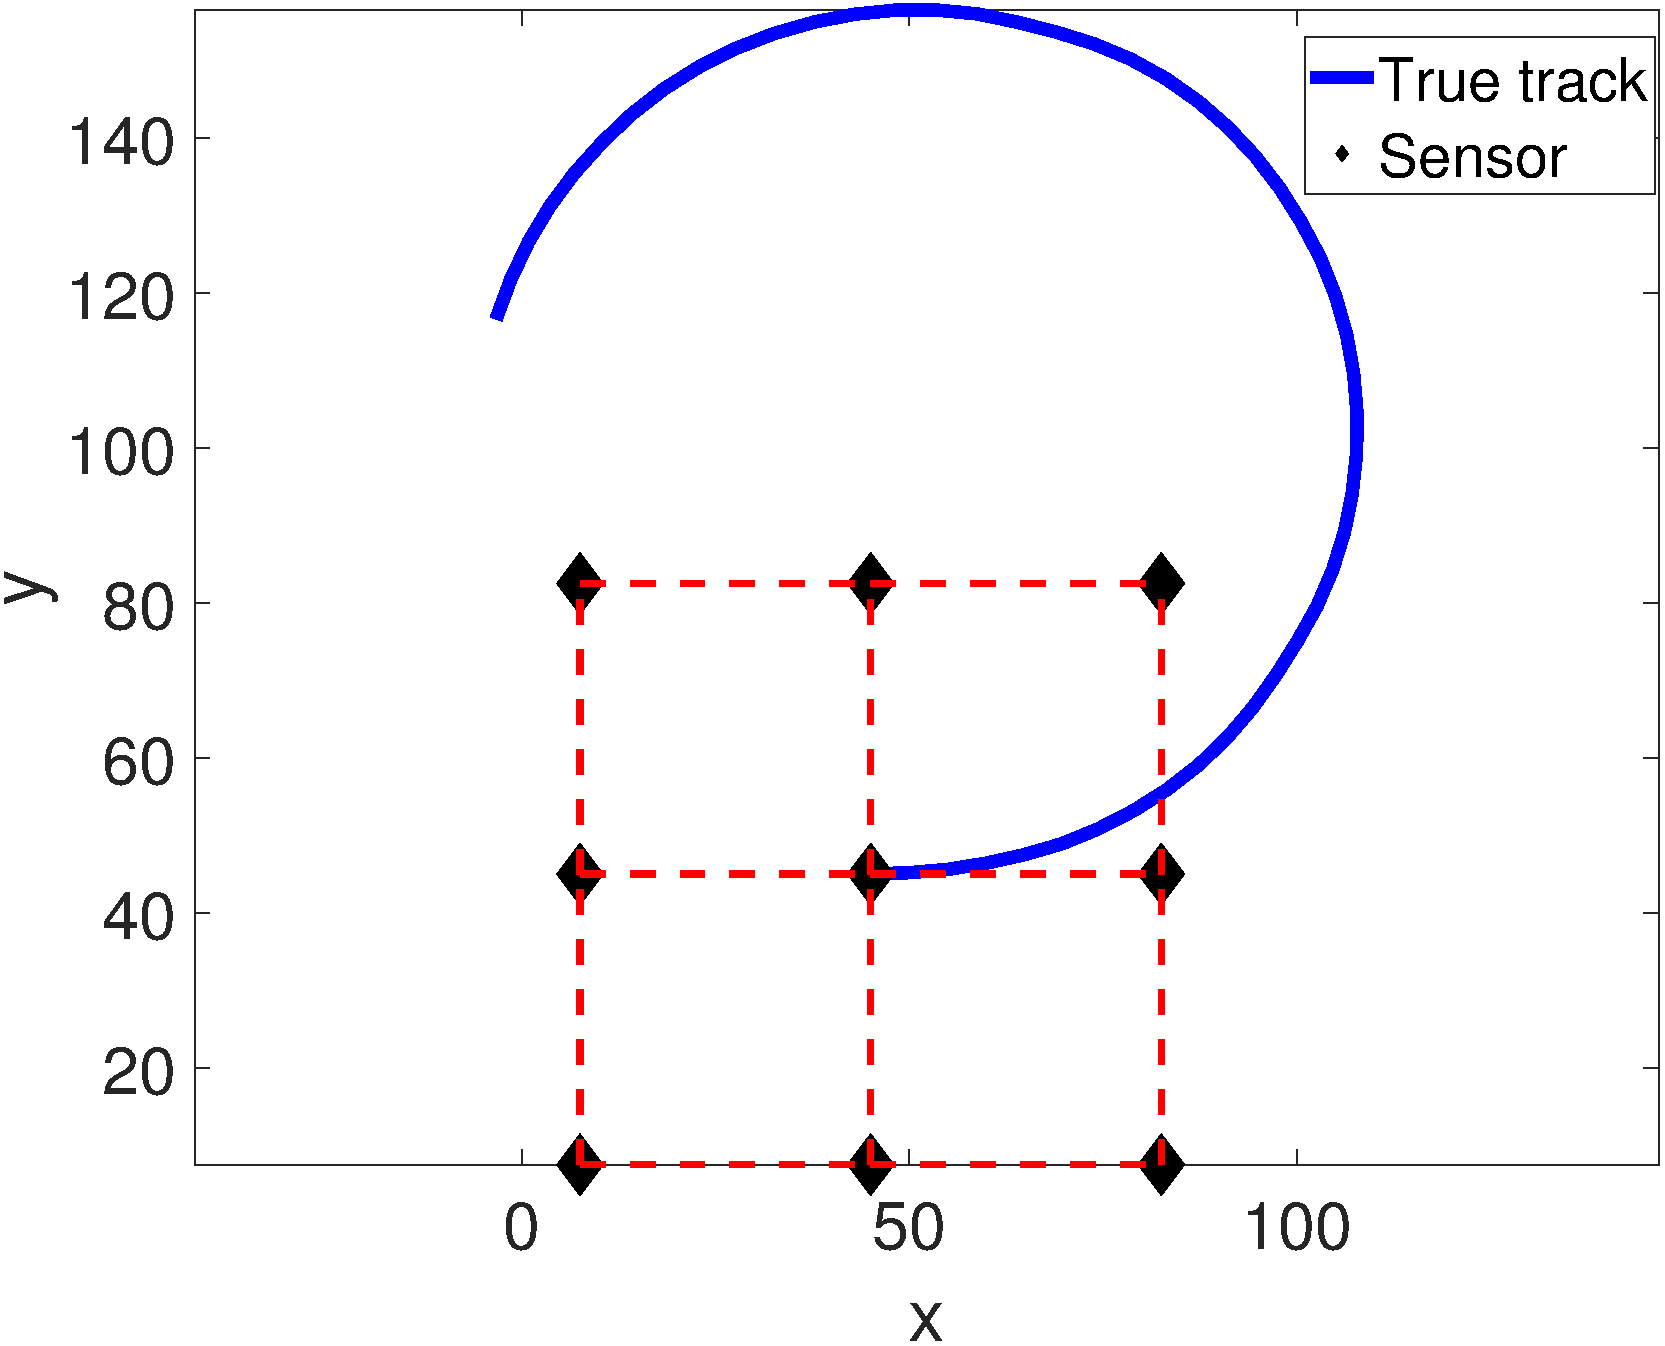
\includegraphics[width=0.45\textwidth]{Figures/track}
%\caption{Target trajectory (blue curve) and sensor positions (black diamond). Sensors connected by red dashed lines are within broadcast range of each other.}
%\label{fig:track}
%\end{figure}

\subsection{Algorithm setup}
All particle filters use a total of $N=500$ particles. At time step 1, we generate the initial particles using the true target state: $X_i(1) \sim \mathcal{N}(X(1), R_{\text{initial}})$ with $R_{\text{initial}}=\text{diag}([0.5^2,0.5^2,0.05^2,0.05^2])$. 

For LCpf, we use a set of basis functions involving all permutations of $x_t^iy_t^j$ with $0\leq i, j \leq d$ where $d$ is some user-specified max degree. (i.e., For $d=2$, the basis functions would be $\beta_1(X) = x_t^0 y_t^0 = 1, \beta_2(X) = x_t^0 y_t^1 = y_t, ..., \beta_9(X) = x_t^2 y_t^2 $.) Note that, due to our choice of basis functions, all particles must remain synchronized across all sensors as in the case of LApf and Clusterpf. For LApf, we construct a DT graph and retain $m< N$ eigenvectors as the basis of Laplacian transformation. For Clusterpf, all particles are grouped into $C$ clusters and a DT graph is constructed to recover individual particle weights. 

The random number generators are synchronized to ensure that the particles remain the same across sensors. Distributed summation is performed using gossip algorithms. At each time step, we perform $NGossip$ gossip iterations. At each gossip iteration, each sensor $i$ broadcasts its local values $G_i$, receives broadcasts from its neighbors, and then updates its local values as a weighted aggregate:
\begin{align}
G_{i,\text{new}} &= w_{ii}G_{i,\text{old}} + \sum_{j\in N_i}w_{ij}G_{j,\text{old}} \\
w_{ij} &=
\begin{cases}
\frac{1}{1+max(d_i, d_j)} \quad j\in N_i \\
1-\sum_{j\in N_i}w_{ij} \quad i=j \\
0 \quad j\notin N_i
\end{cases}
\label{eqn:metropolis_weight}
\end{align}
where $N_i$ denotes the set of neighboring sensors of sensor $i$, $d_i=|N_i|$, and Metropolis weight is used for the update. After a total of $NGossip$ iterations, a max consensus algorithm is run to ensure all sensors obtain the same values. 

In our codes, we do not implement a loop for the gossip iterations. Instead we define an update matrix $W$ where $W(i,j)=w_{ij}$. Therefore, given initial values $G_{\text{initial}}=[G_1,...,G_S]^T$, the final values can be easily computed as 
\begin{equation}
G_{\text{final}} = W^{NGossip}G_{\text{initial}}
\end{equation}

In the remainder of the section, we run a number of Monte Carlo simulations to evaluate the performance of the four filters. The track remains the same in each trial; but the measurements differ. We evaluate the algorithms' performances using the \textit{root mean squared error} (RMSE) of position estimate and discrepancy of normalized particle weights, $||w_{\text{true}}-w_{\text{approx}}||_2$, averaged over all time steps and all trials. The first metric is self-explanatory and the second metric is meant to evaluate the impact of different filters' encoding scheme on the overall tracking performance.

%, and \textit{aggregate error ratio} (AER). The first metric is self-explanatory; so we will only explain the last one. Let $G_{gossip}$ denote the vector of the approximate aggregate values computed using gossip and max consensus, and let $G_{exact}$ denote the vector of exact aggregate values. We compute the ratio vector $|\frac{G_{gossip}-G_{exact}}{G_{exact}}|$ and report the average ratio. Ideally, for $NGossip$ approaching infinity, the ratio approaches 0 as the approximate value approaches the exact value. 

%\subsection{Constraint sufficient statistics particle filter}
%Consider first CSSpf. Each sensor needs to broadcast $6NGossip$ scalars at each time step. We thus study the trade-off between communication overhead and tracking performance. Fig.~\ref{fig:results_CSSpf} shows the boxplots of RMSE and AER with respect to number of gossip iterations for different values of $N$. %Each data point is averaged over 50 time steps and 200 Monte Carlo trials. 
%
%The RMSE is very high for $NGossip< 20$ which can be attributed to the gossip algorithm not converging in such few iterations and having high errors in the final values of the global sufficient statistics. For $NGossip\geq 20$, the RMSE is fairly constant and more gossip iterations and more particles do not yield significant improvement in tracking performance. 
%
%With increasing $NGossip$, the AER decreases exponentially (note the log-scale of the Y-axis) and drops sharply for $NGossip \geq 50$. For $NGossip=20$, the ratio drops close to 0.02 which is low enough to yield adequate tracking performance. For higher values of $NGossip$, the ratio drops even further; although the tracking performance improvement is marginal at best. As $N$ increases, the AER does not change significantly. This is to be expected since the number of sufficient statistics to be aggregated is constant and independent of the number of particles. 
%
%\begin{figure}
%\centering
%\begin{subfigure}[RMSE]
%{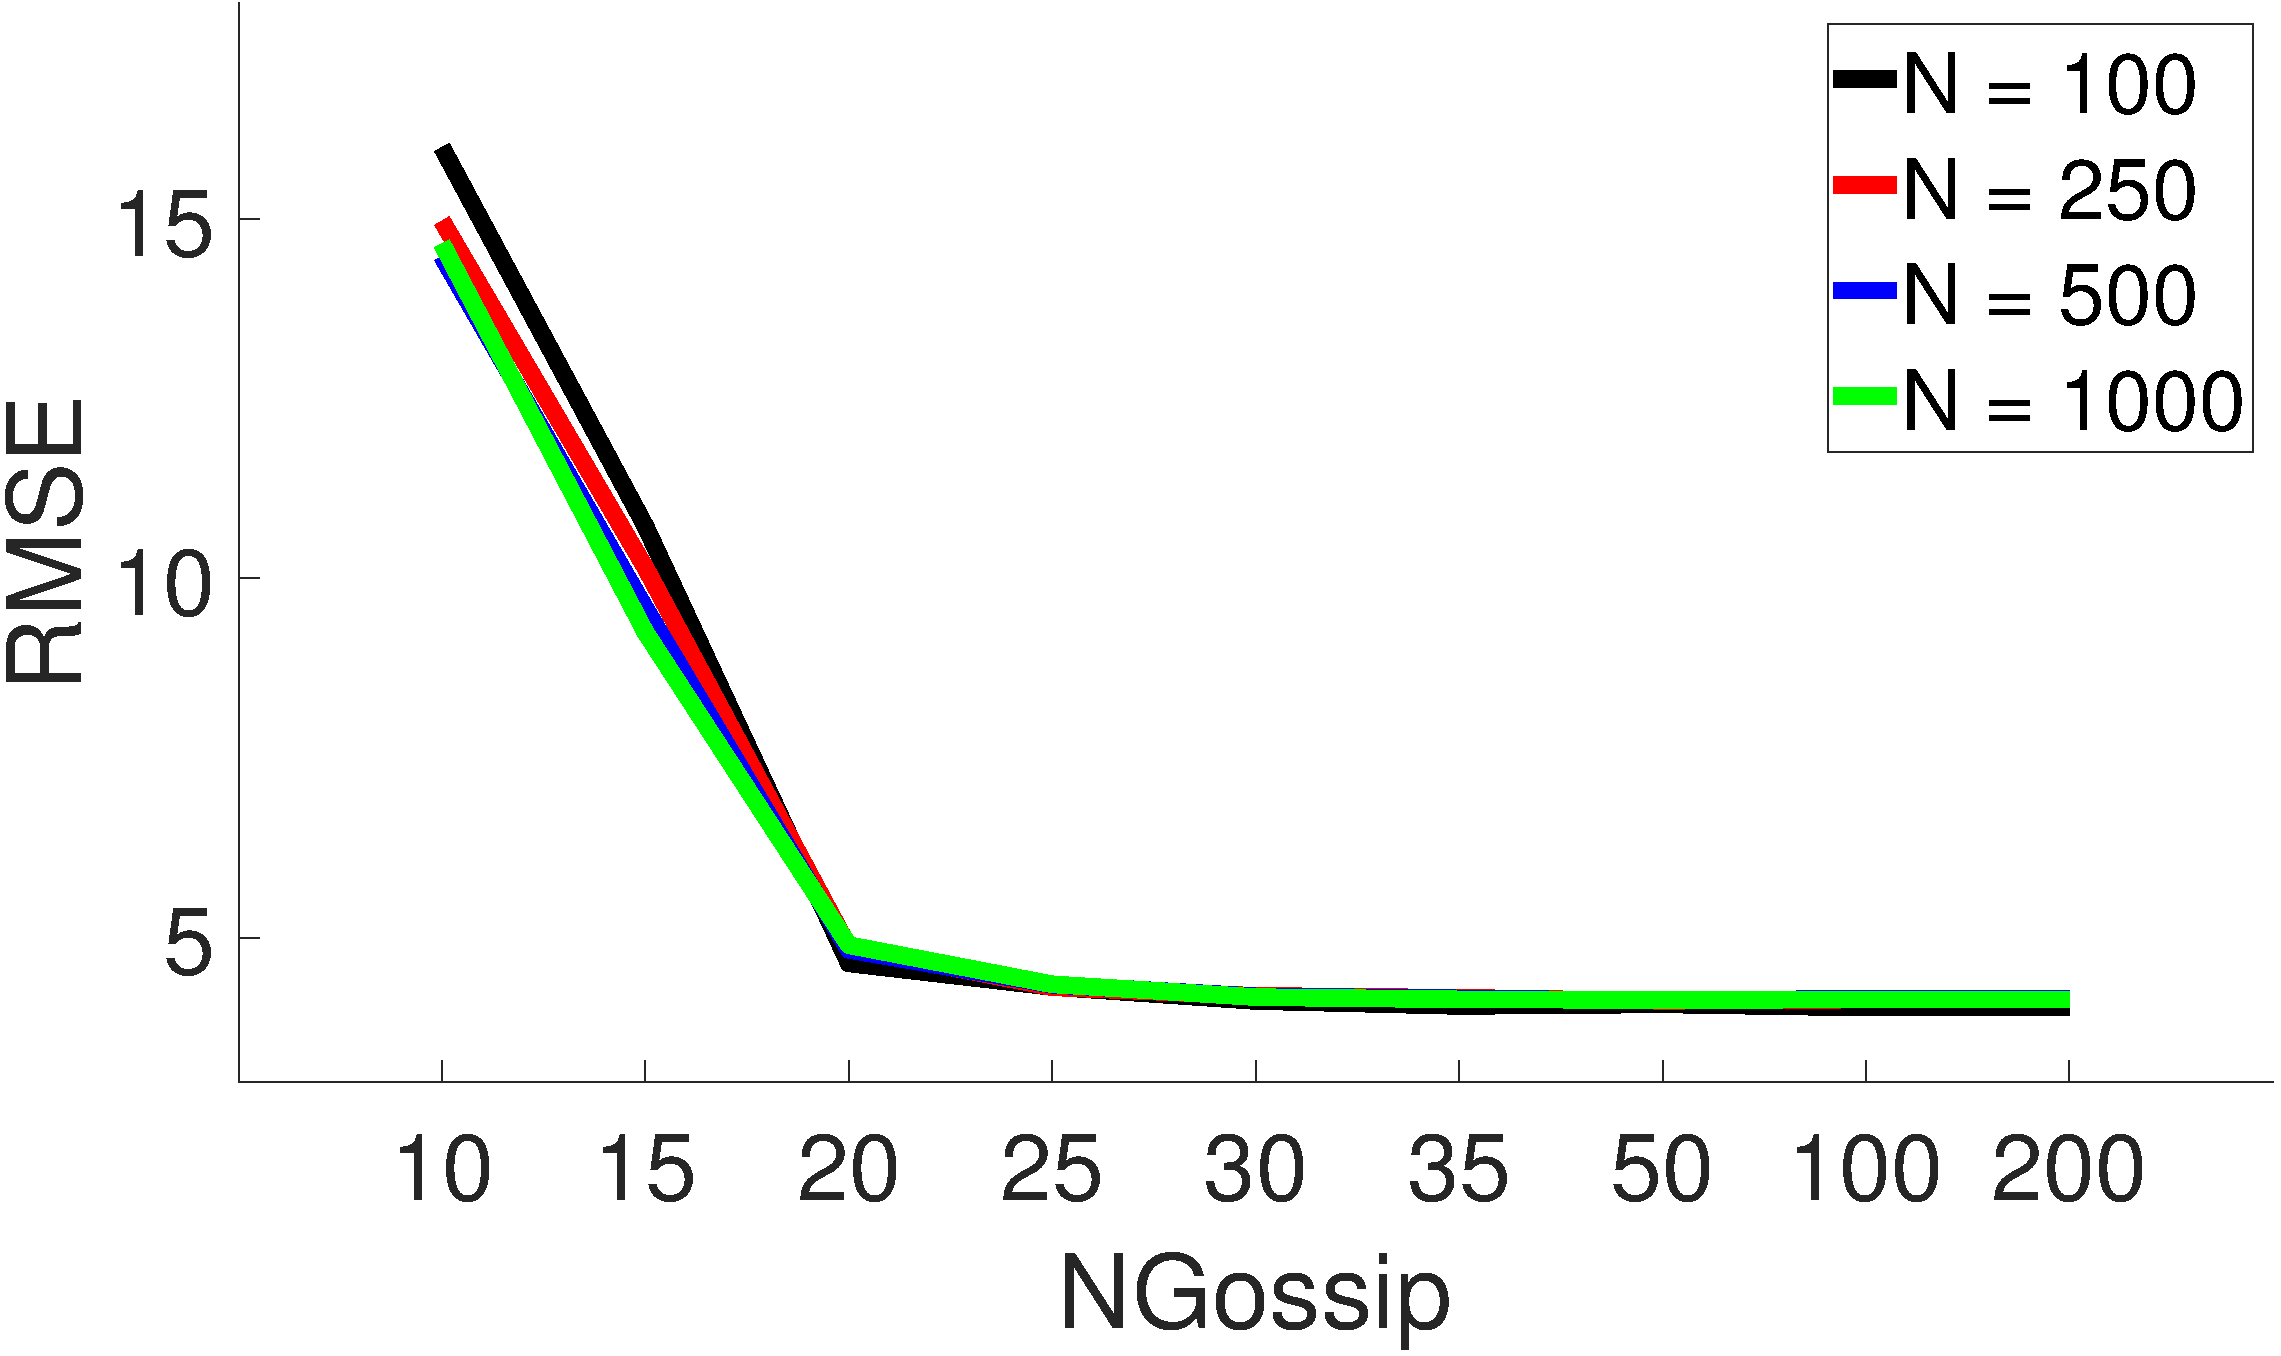
\includegraphics[width=0.49\textwidth]{Figures/curve_CSSpf_RMSE}}
%\end{subfigure}
%%\begin{subfigure}[total runtime]
%%{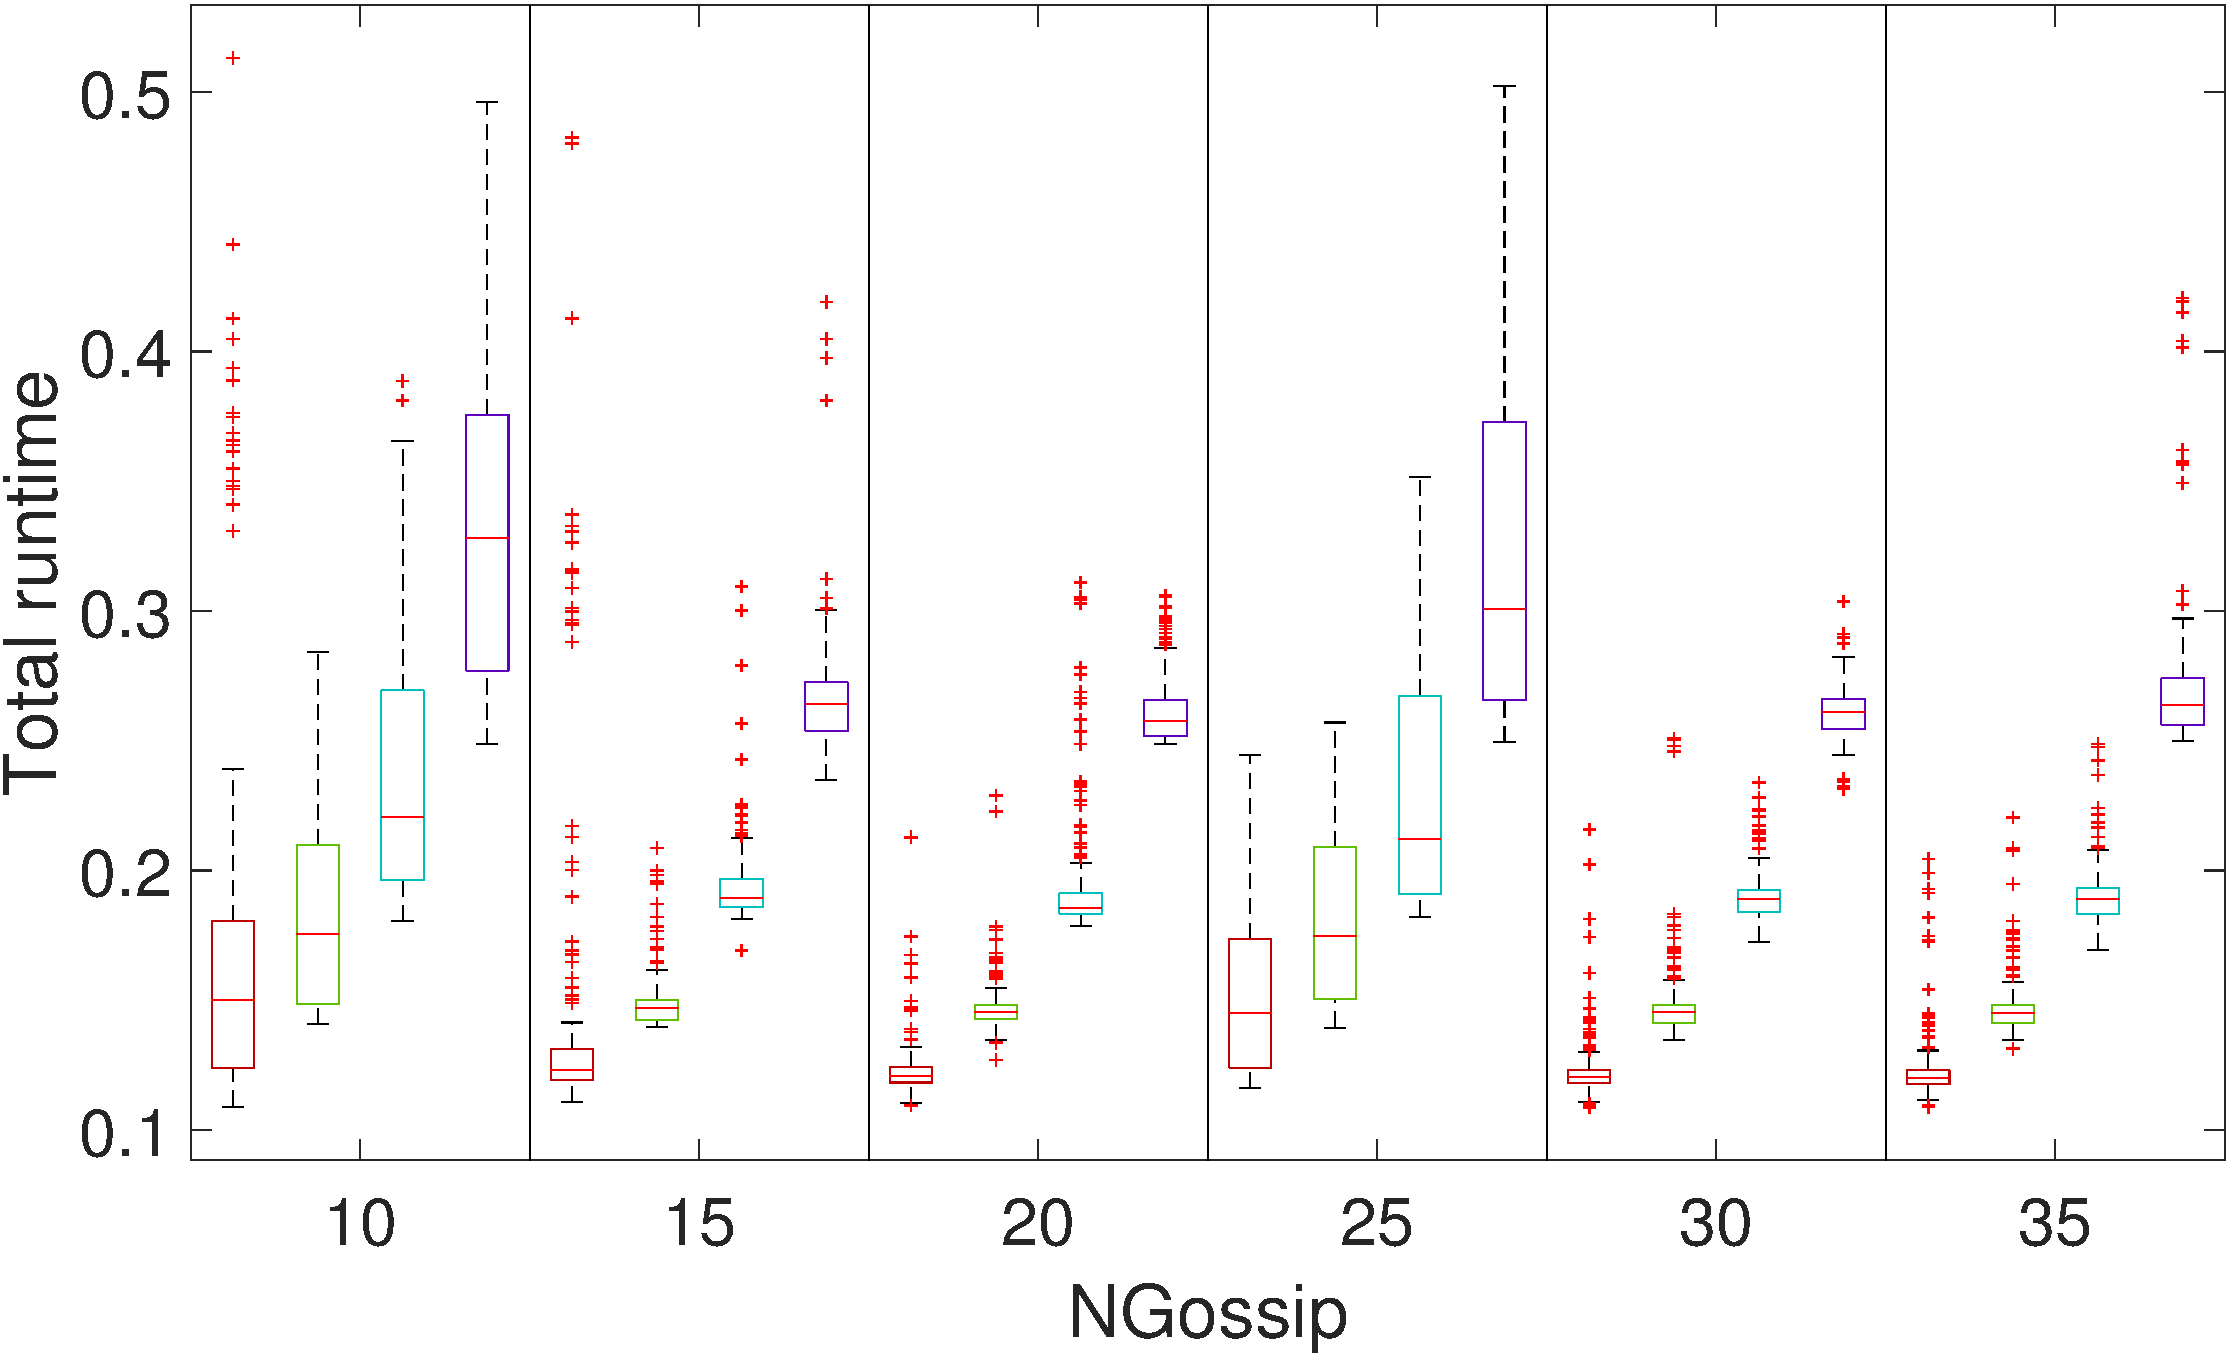
\includegraphics[width=0.65\textwidth]{Figures/boxplot_CSSpf_time}}
%%\end{subfigure}
%\begin{subfigure}[AER]
%{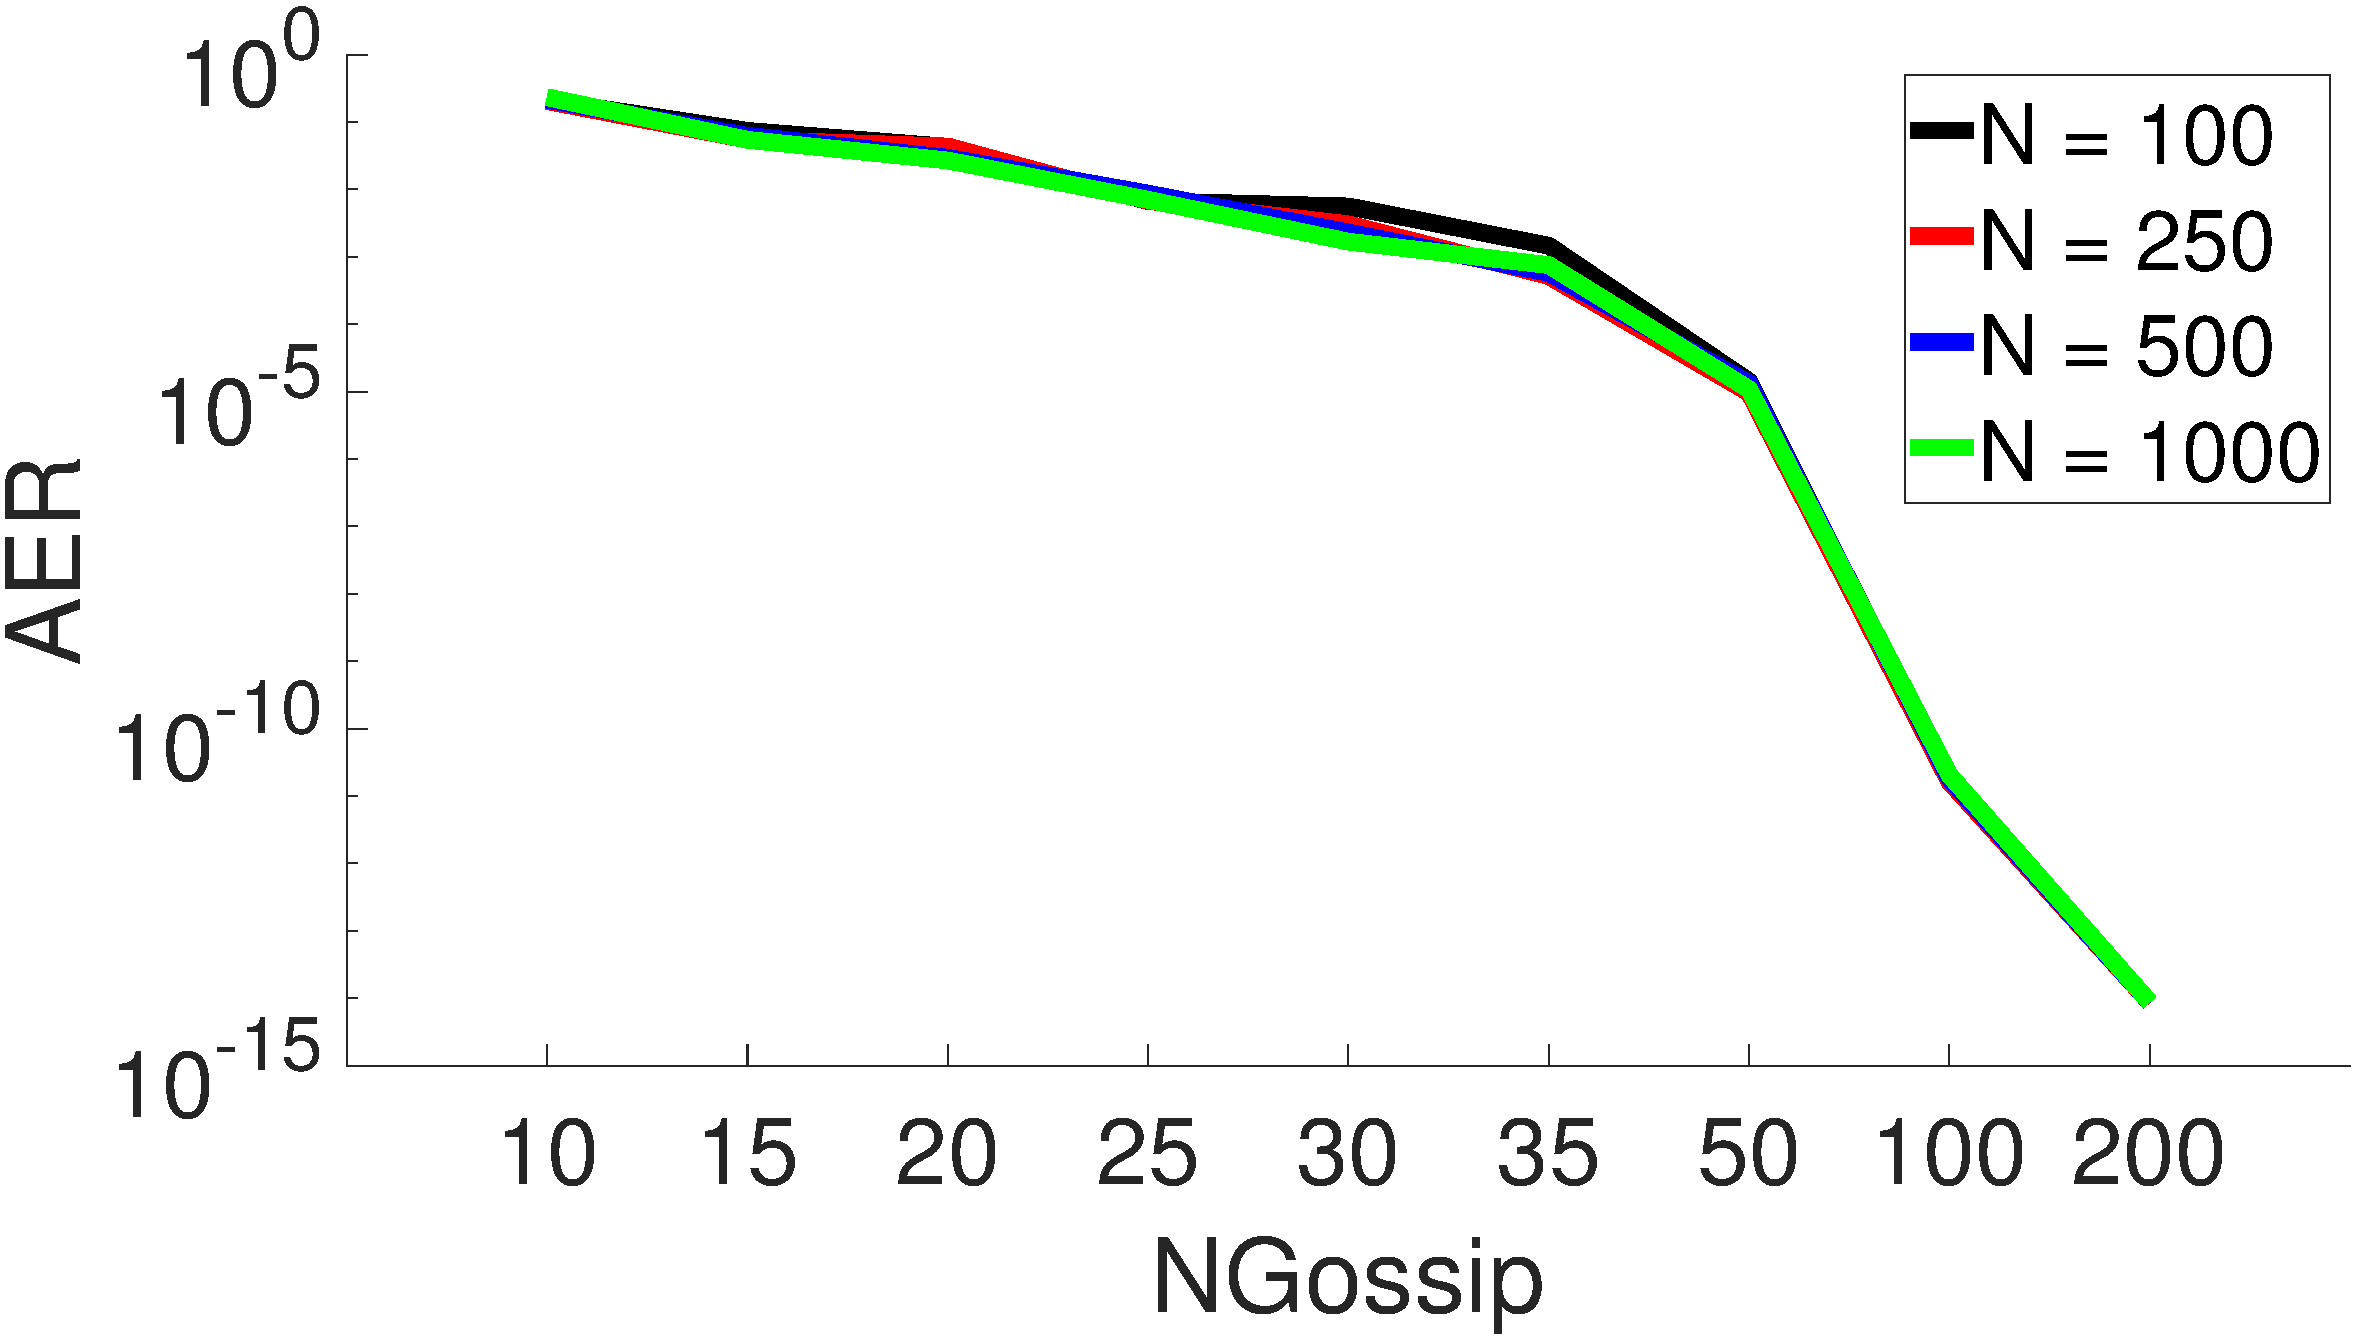
\includegraphics[width=0.49\textwidth]{Figures/curve_CSSpf_AER}}
%\end{subfigure}
%\caption{RMSE and AER of CSSpf with respect to $NGossip$ for different values of $N$. Each data point is averaged over 50 time steps and 200 Monte Carlo trials.}
%\label{fig:results_CSSpf}
%\end{figure}
%
%\subsection{Likelihood consensus particle filter}
%The max degree $d$ offers a trade-off between tracking performance and computational/communication overhead. Higher degree $d$ generates more basis functions and should yield better approximation of the measurement model. On the other hand, more basis functions lead to more computation, more communication and longer runtime. In fact, the total number of basis functions $J$ grows exponentially at $O(d^2)$. 
%
%Fig.~\ref{fig:results_LCpf_maxDegree} shows the boxplots of RMSE with respect to $d$. Note that, for this particular set of trials, all summations are computed exactly without gossiping. For all values of $d>1$, the RMSE remains fairly constant. This suggests that additional basis functions from $d>2$ do not improve the approximation of the measurement model $H(X_i)$ by any significant margin. To verify our conjecture, we compute the following metric. Let $W_{\text{true}}$ denote the true particle weights and let $W_{\text{approx}}$ denote the approximate weights. We compute and report $||W_{\text{true}}-W_{\text{approx}}||_2$ in Fig.~\ref{fig:boxplot_LCpf_weight_approx_error}. With the exception of $d=1$, the weight error is fairly constant. These results suggest that $d=2$ is sufficient to yield adequate tracking performance while minimizing computational overhead. 
%
%\begin{figure}
%\centering
%\begin{subfigure}[RMSE]
%{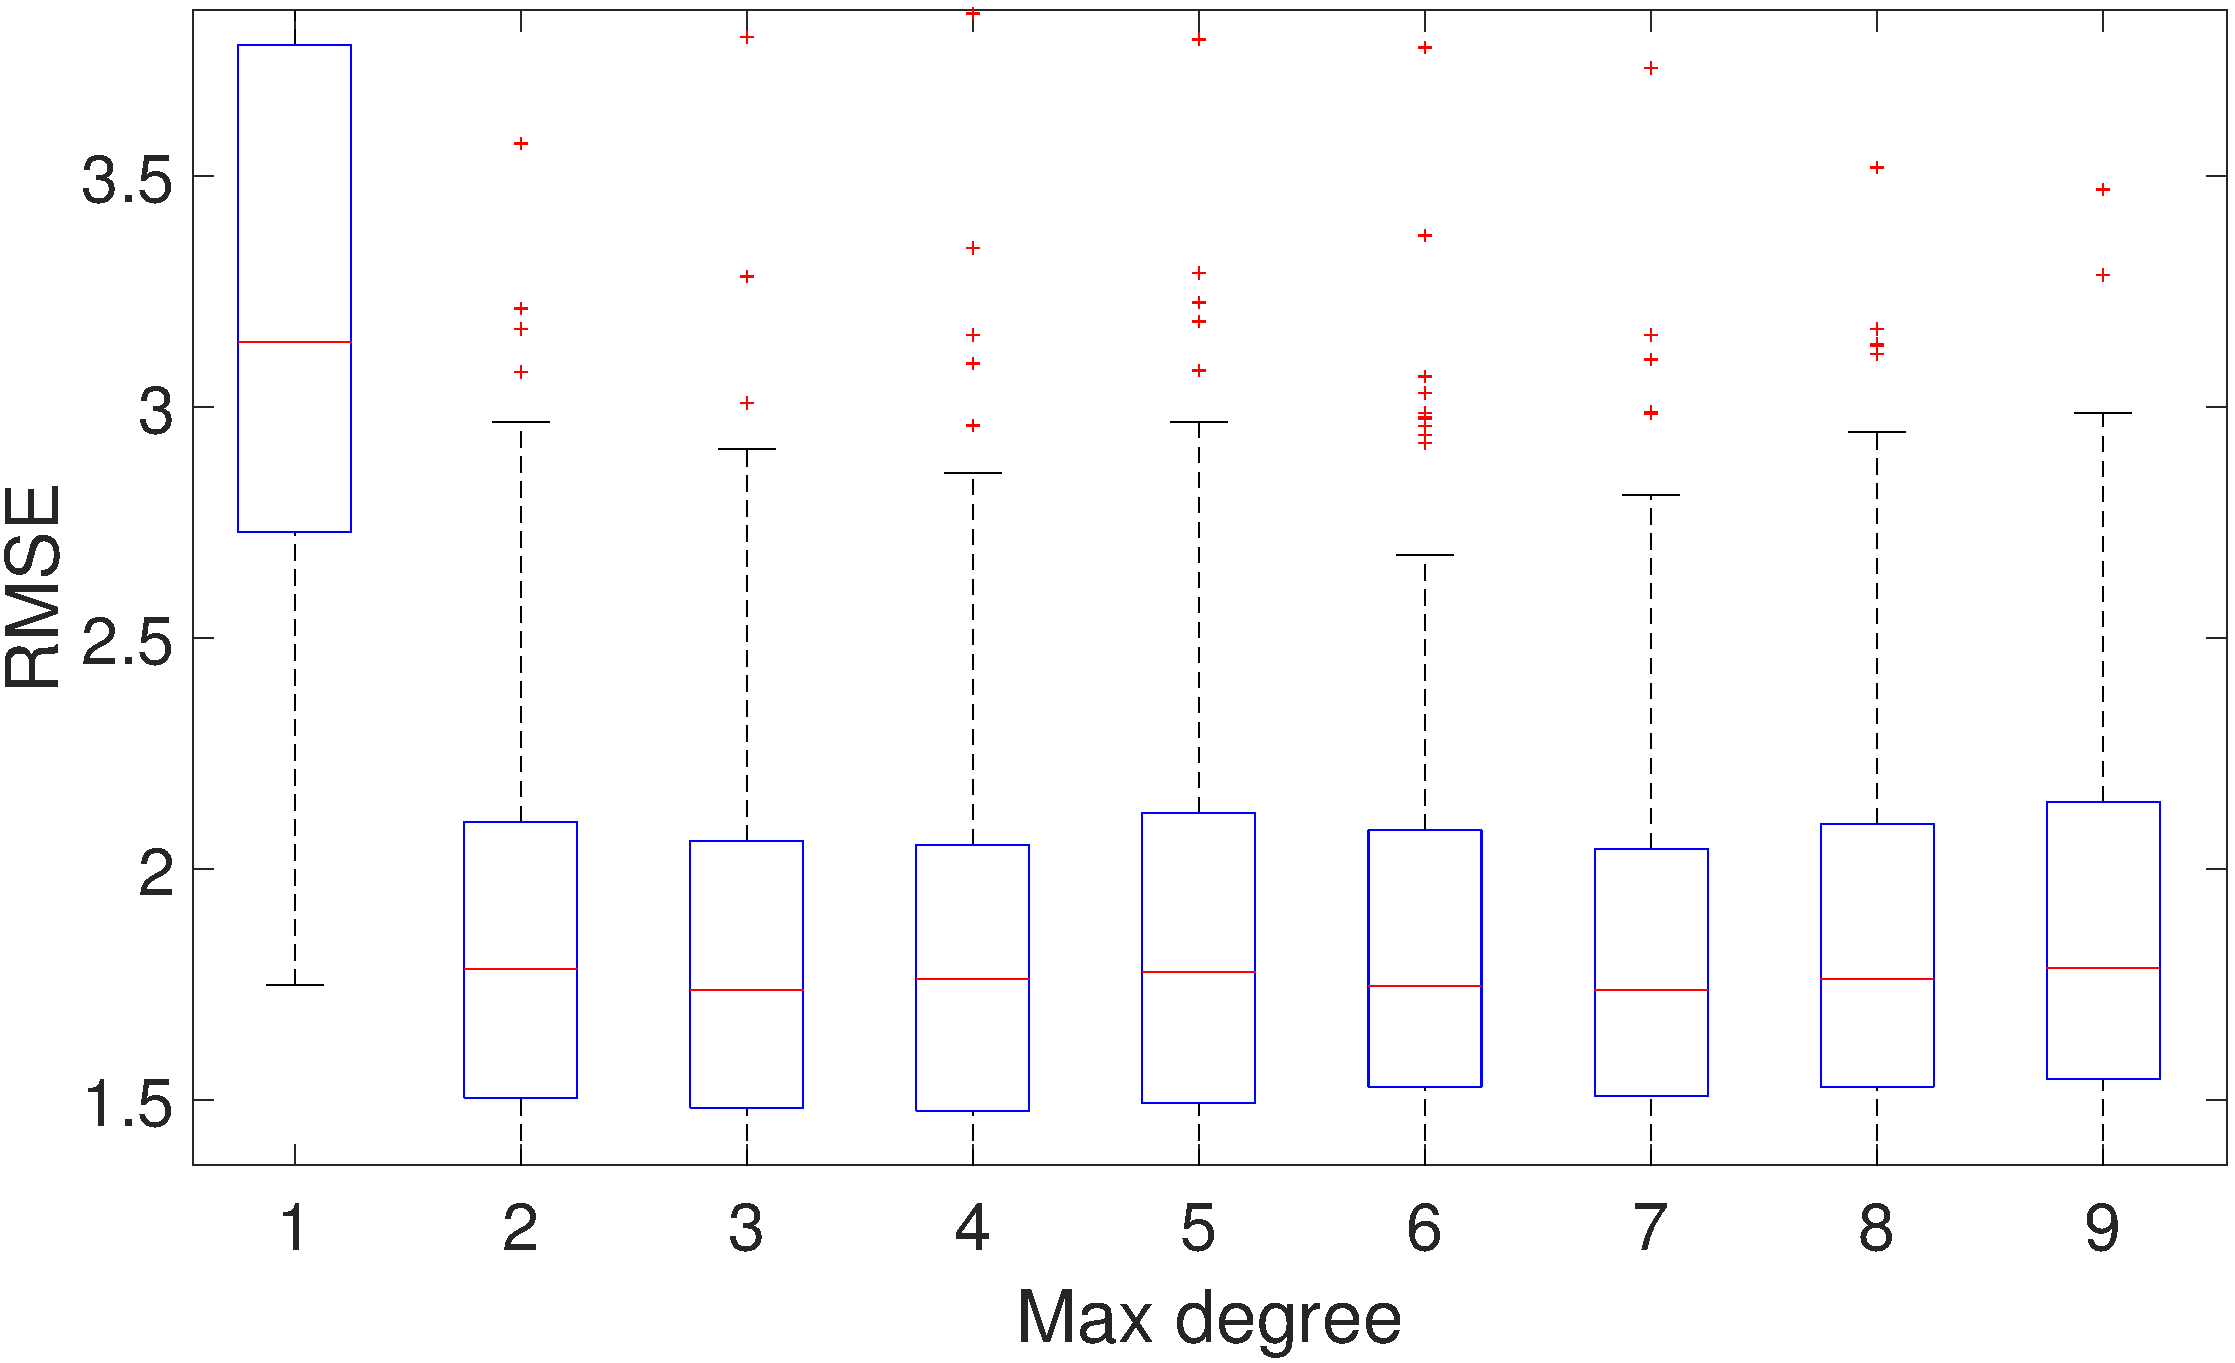
\includegraphics[width=0.47\textwidth]{Figures/boxplot_LCpf_RMSE_maxDegree}
%\label{fig:results_LCpf_maxDegree}}
%\end{subfigure}
%\begin{subfigure}[Measurement approximation error]
%{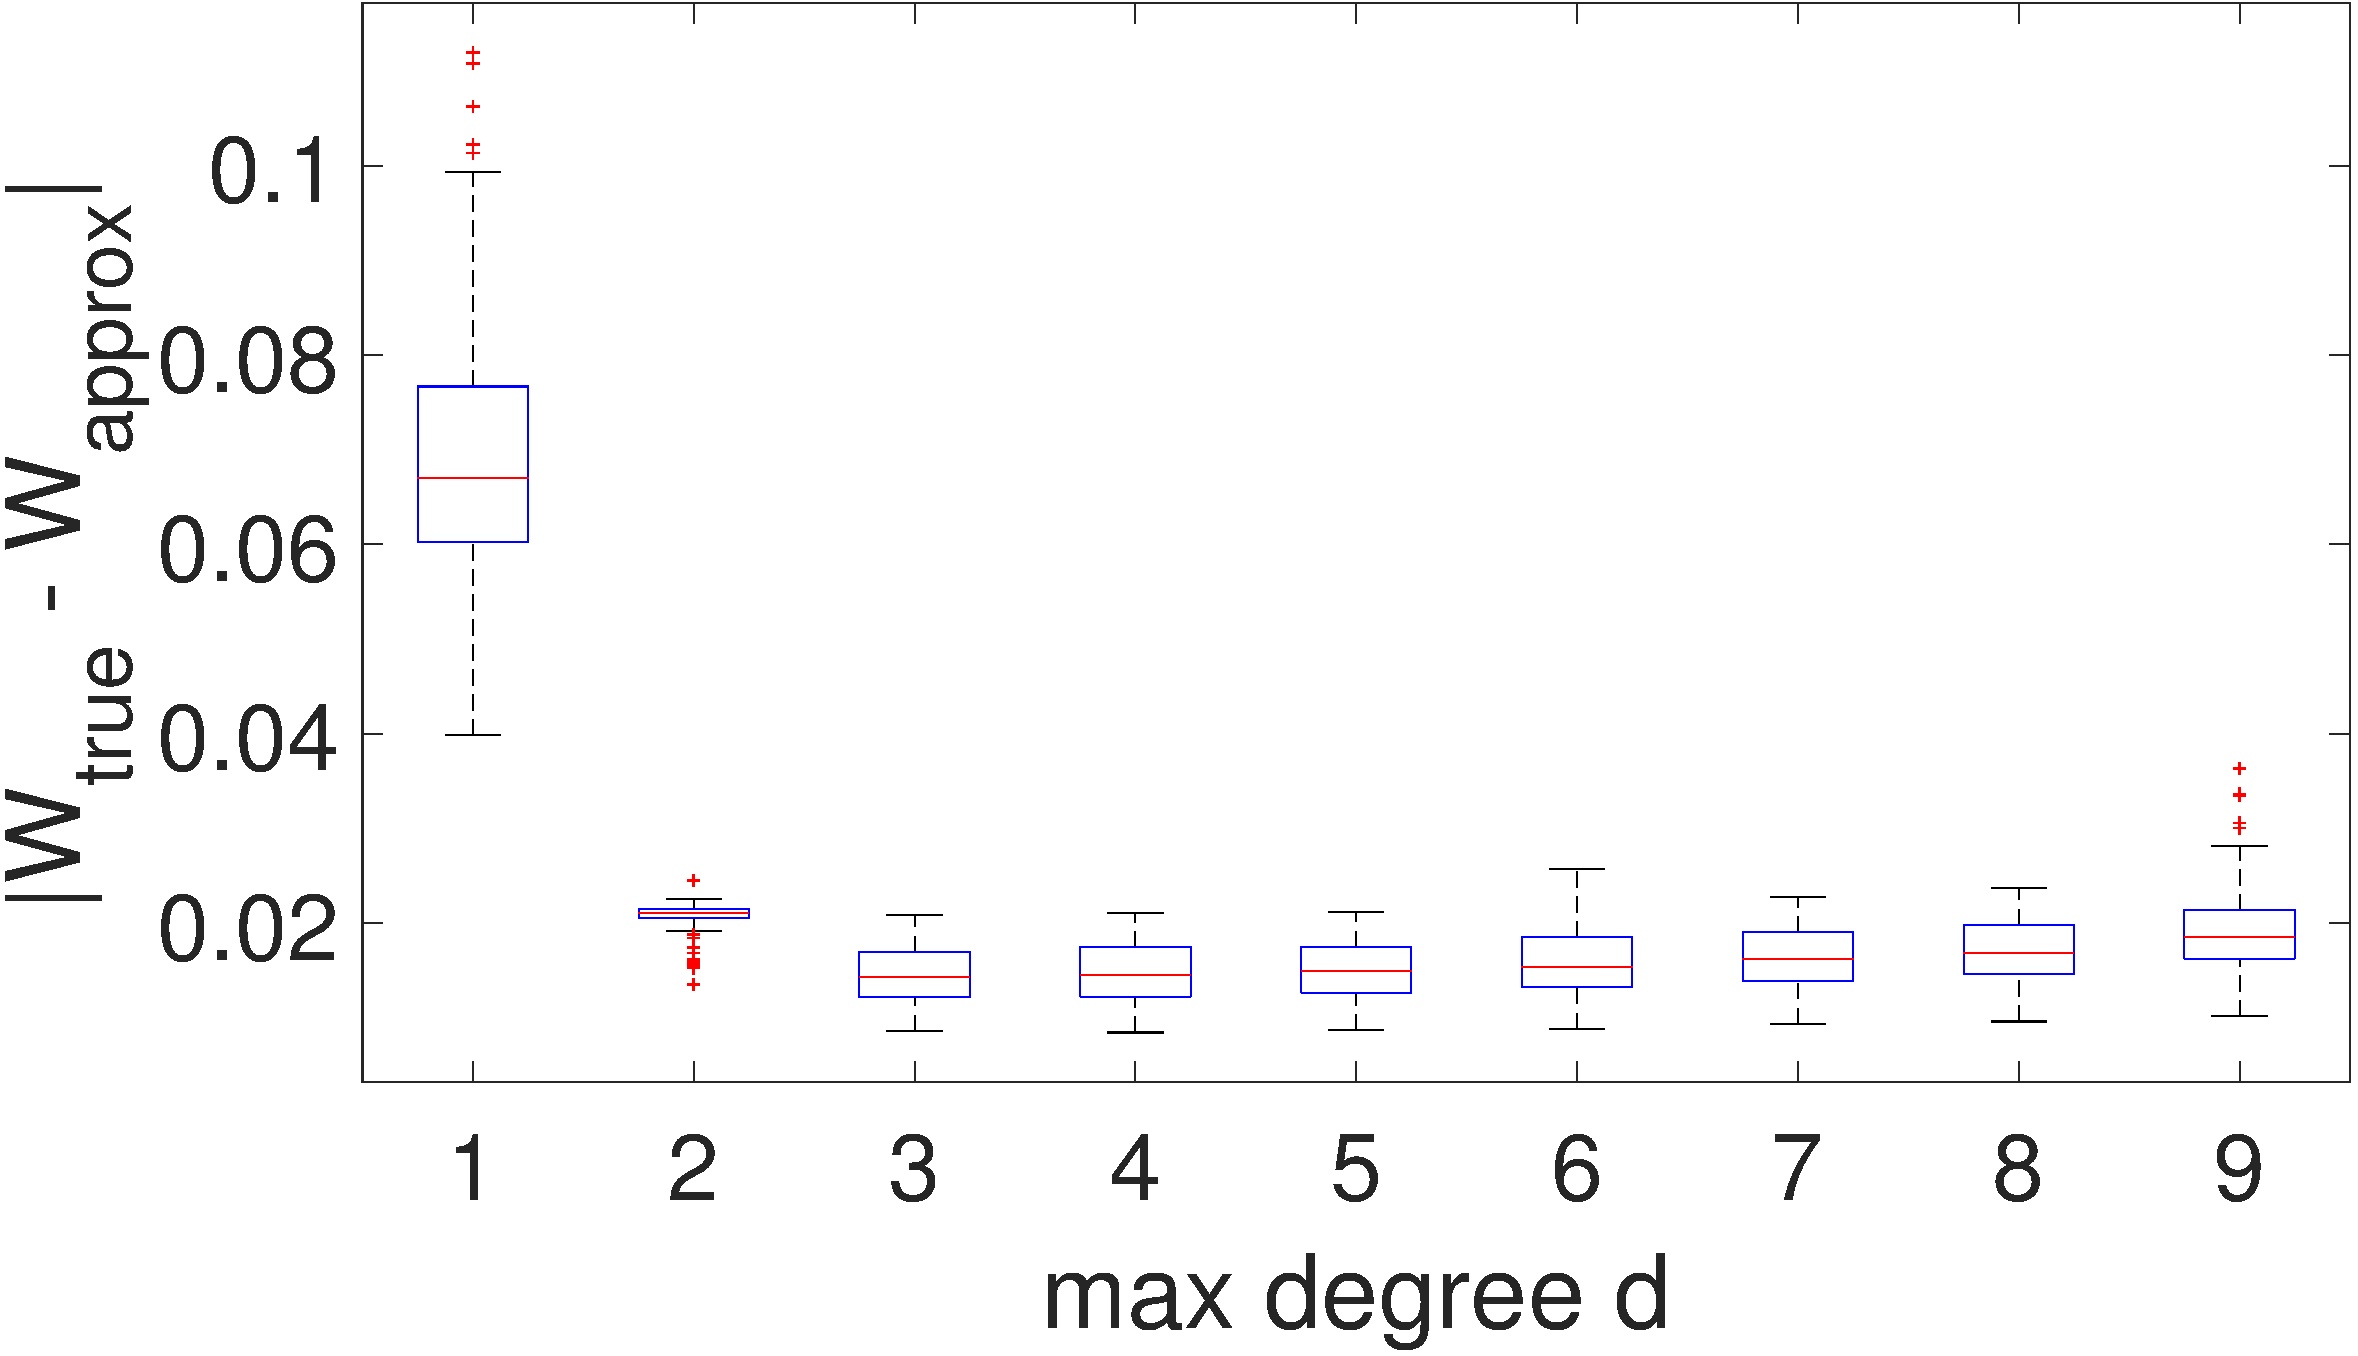
\includegraphics[width=0.47\textwidth]{Figures/boxplot_LCpf_weight_approx_error_maxDegree}\label{fig:boxplot_LCpf_weight_approx_error}}
%\end{subfigure}
%\caption{Boxplot of RMSE and average weight approximation error of LCpf with respect to $d$. All summations are computed exactly without gossip. $N=500$}
%\end{figure}
%
%\begin{figure}
%\centering
%\begin{subfigure}[RMSE]
%{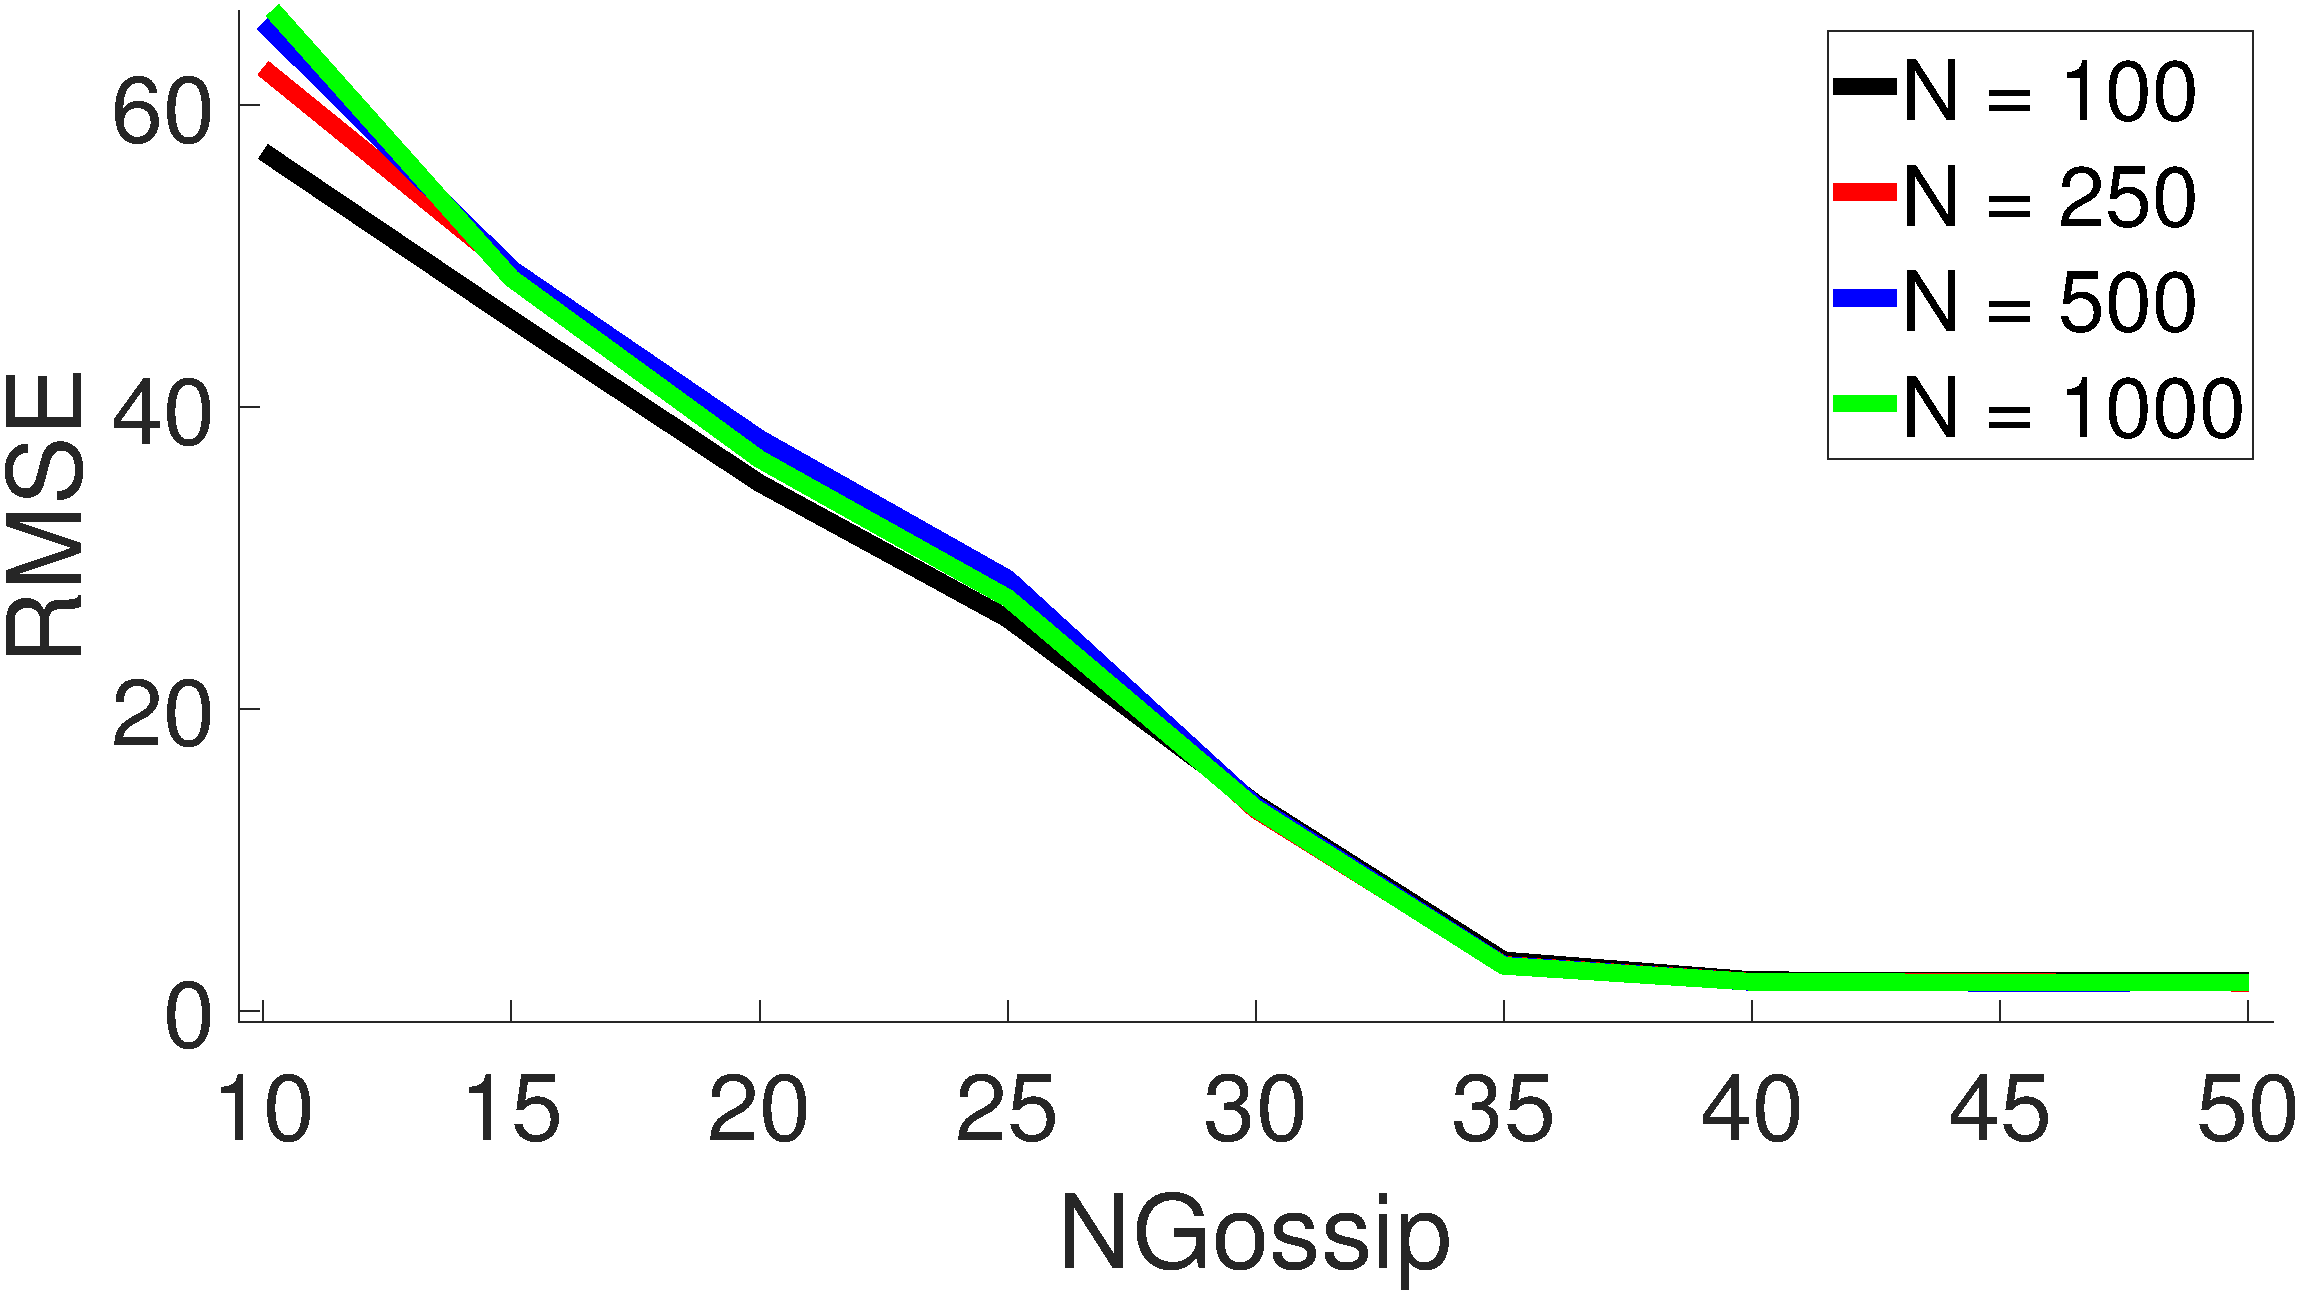
\includegraphics[width=0.49\textwidth]{Figures/curve_LCpf_llh_RMSE}}
%\end{subfigure}
%\begin{subfigure}[AER]
%{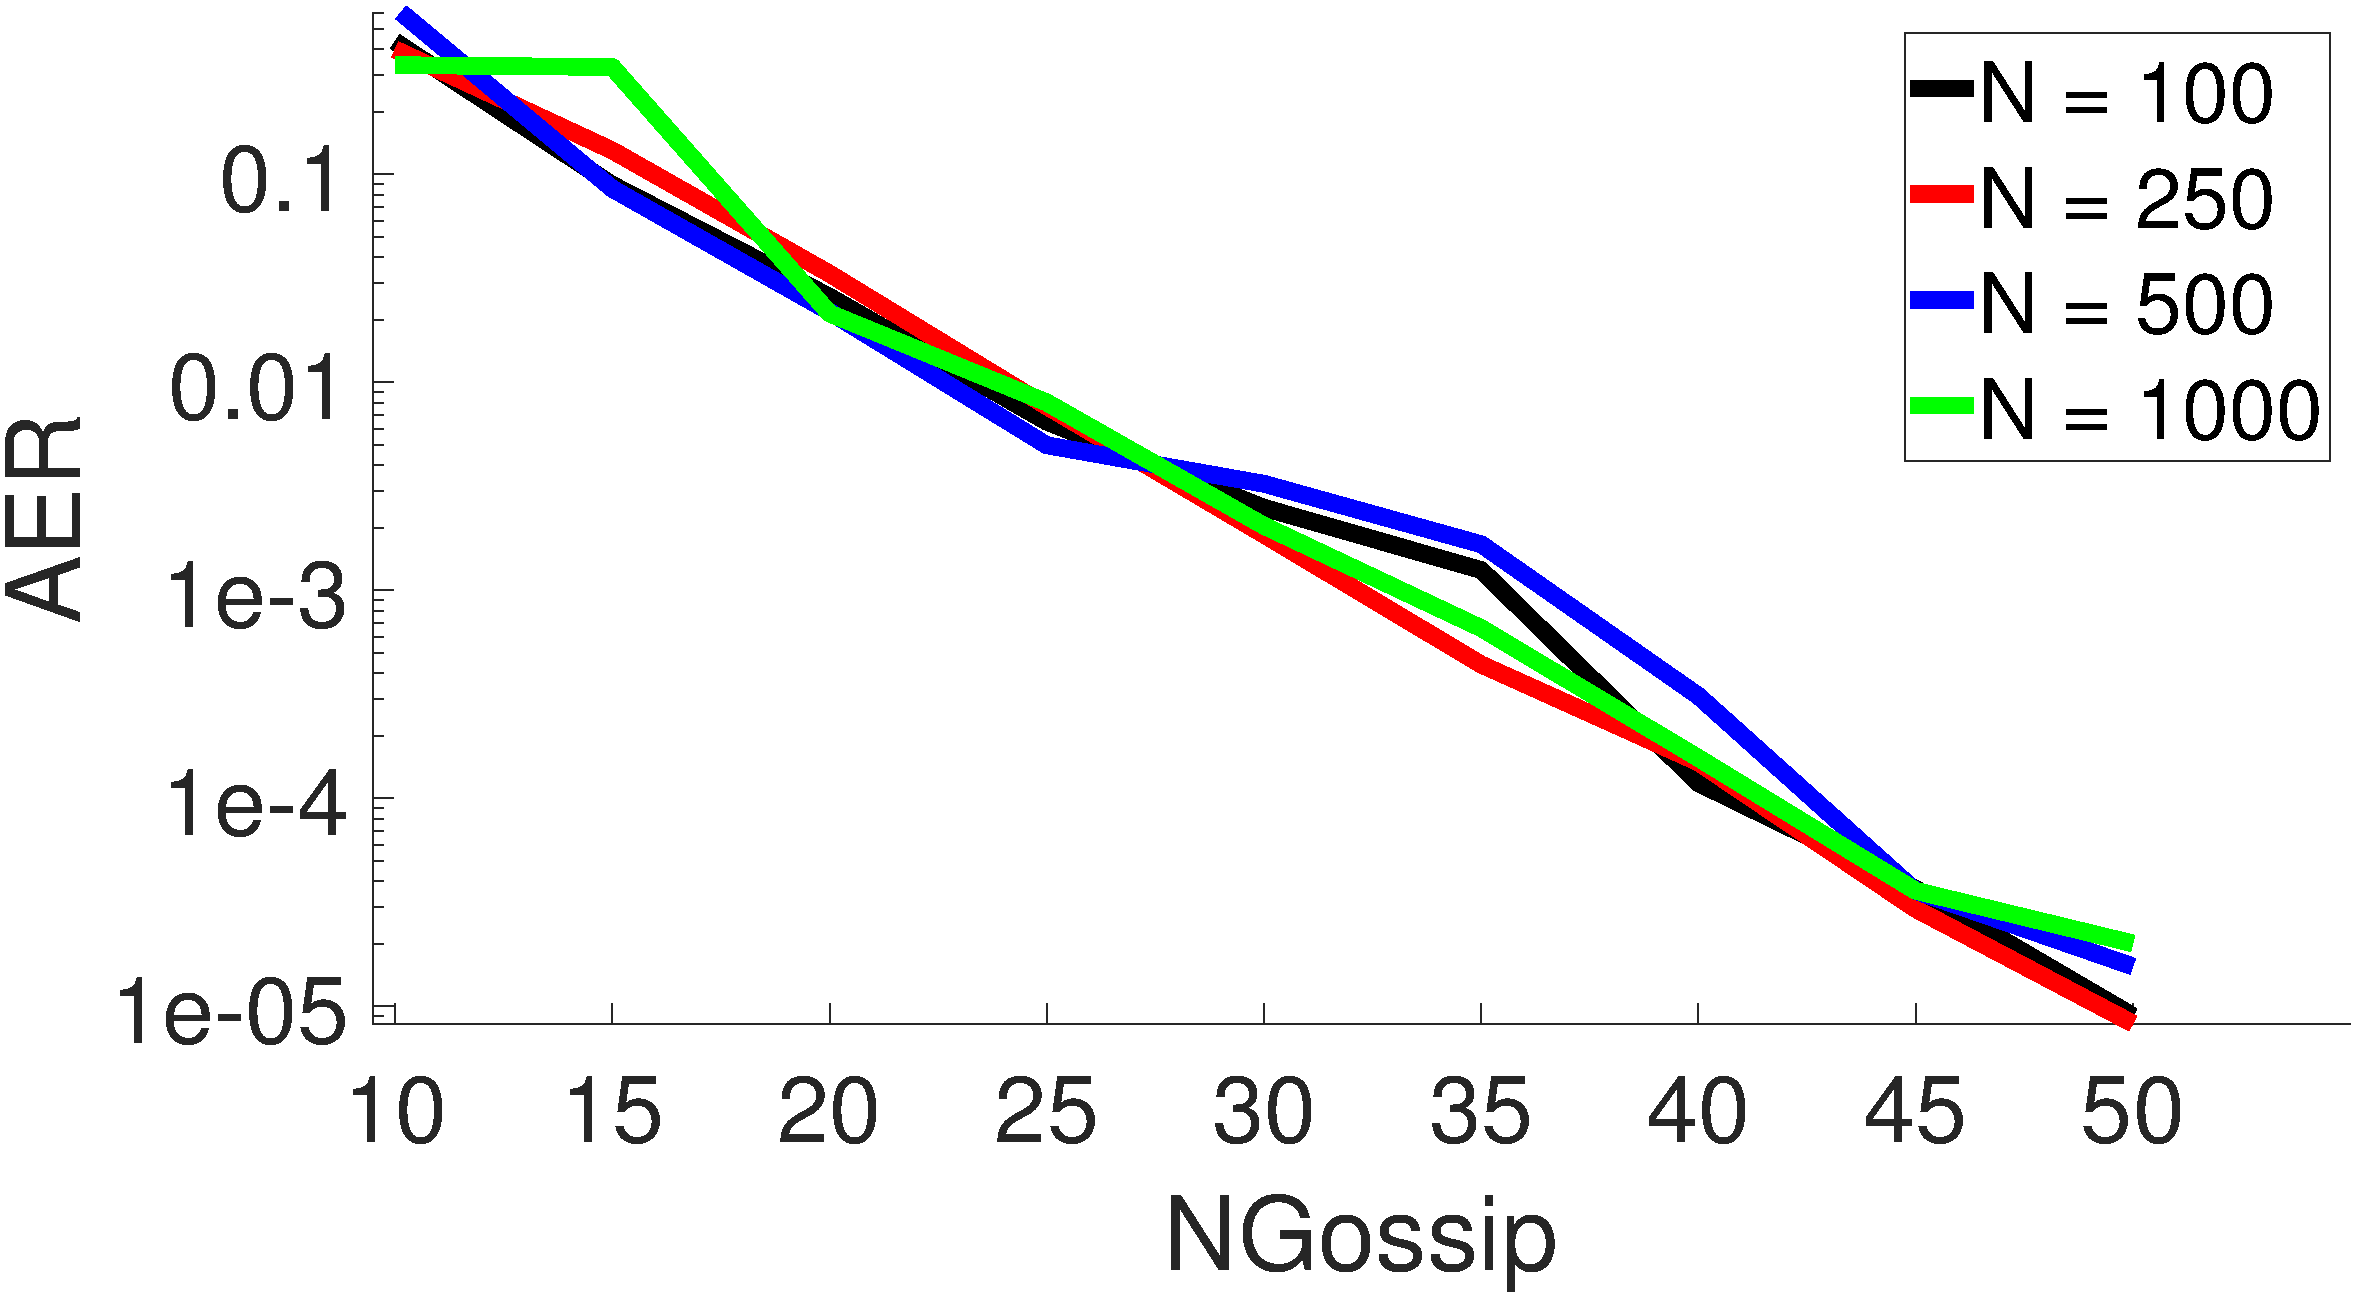
\includegraphics[width=0.49\textwidth]{Figures/curve_LCpf_llh_AER}}
%\end{subfigure}
%\caption{RMSE and AER of LCpf with respect to $NGossip$ for different values of $N$ ($d$=2). All data points are averaged over 50 time steps and 200 Monte Carlo trials.}
%\label{fig:results_LCpf_llh}
%\end{figure}
%
%Fig.~\ref{fig:results_LCpf_llh} shows the average RMSE and AER with respect to number of gossip iterations for $d=2$ and different values of $N$. For LCpf, a minimal of 35 gossip iterations is necessary to yield adequate tracking performance. Furthermore, at $d=2$, each sensor needs to broadcast 9 scalars per gossip iteration. In other words, the communication overhead of LCpf is 3 times that of CSSpf to achieve similar tracking performance as CSSpf. %If we compare Fig. 2(b) and Fig. 4(b), we note that CSSpf and LCpf exhibit very similar level of AER for the same $NGossip$. This suggests that LCpf is significantly more susceptible to error induced by distributed summation. %Furthermore, LCpf requires double the runtime of CSSpf with the total runtime increasing for higher $N$. 
%
%\subsection{Laplacian approximation particle filter}
%The LApf has one parameter of interest: $m$, the number of eigenvectors to encode the particle log-likelihoods. Fig.~\ref{fig:results_LApf} shows the RMSE and AER of LApf with respect to $NGossip$ for different values of $m$ and $N=500$. 
%
%\begin{figure}
%\centering
%\begin{subfigure}[RMSE]
%{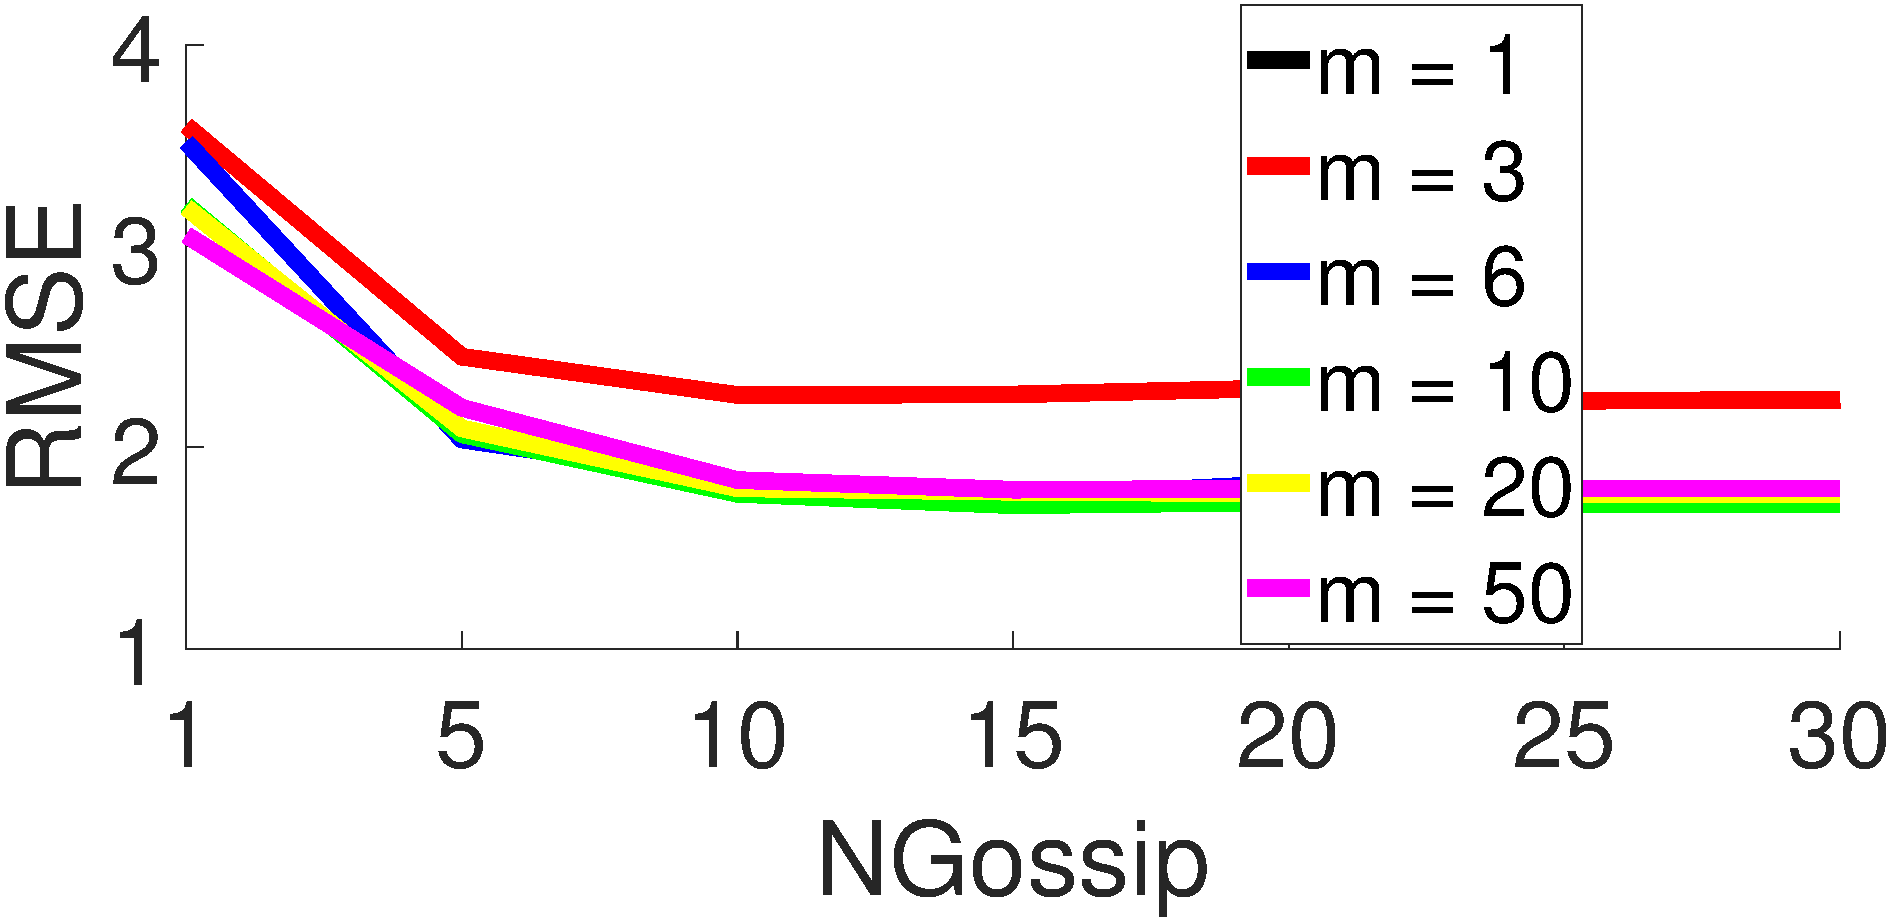
\includegraphics[width=0.47\textwidth]{Figures/curve_LApf_RMSE}}
%\end{subfigure}
%%\begin{subfigure}[total runtime]
%%{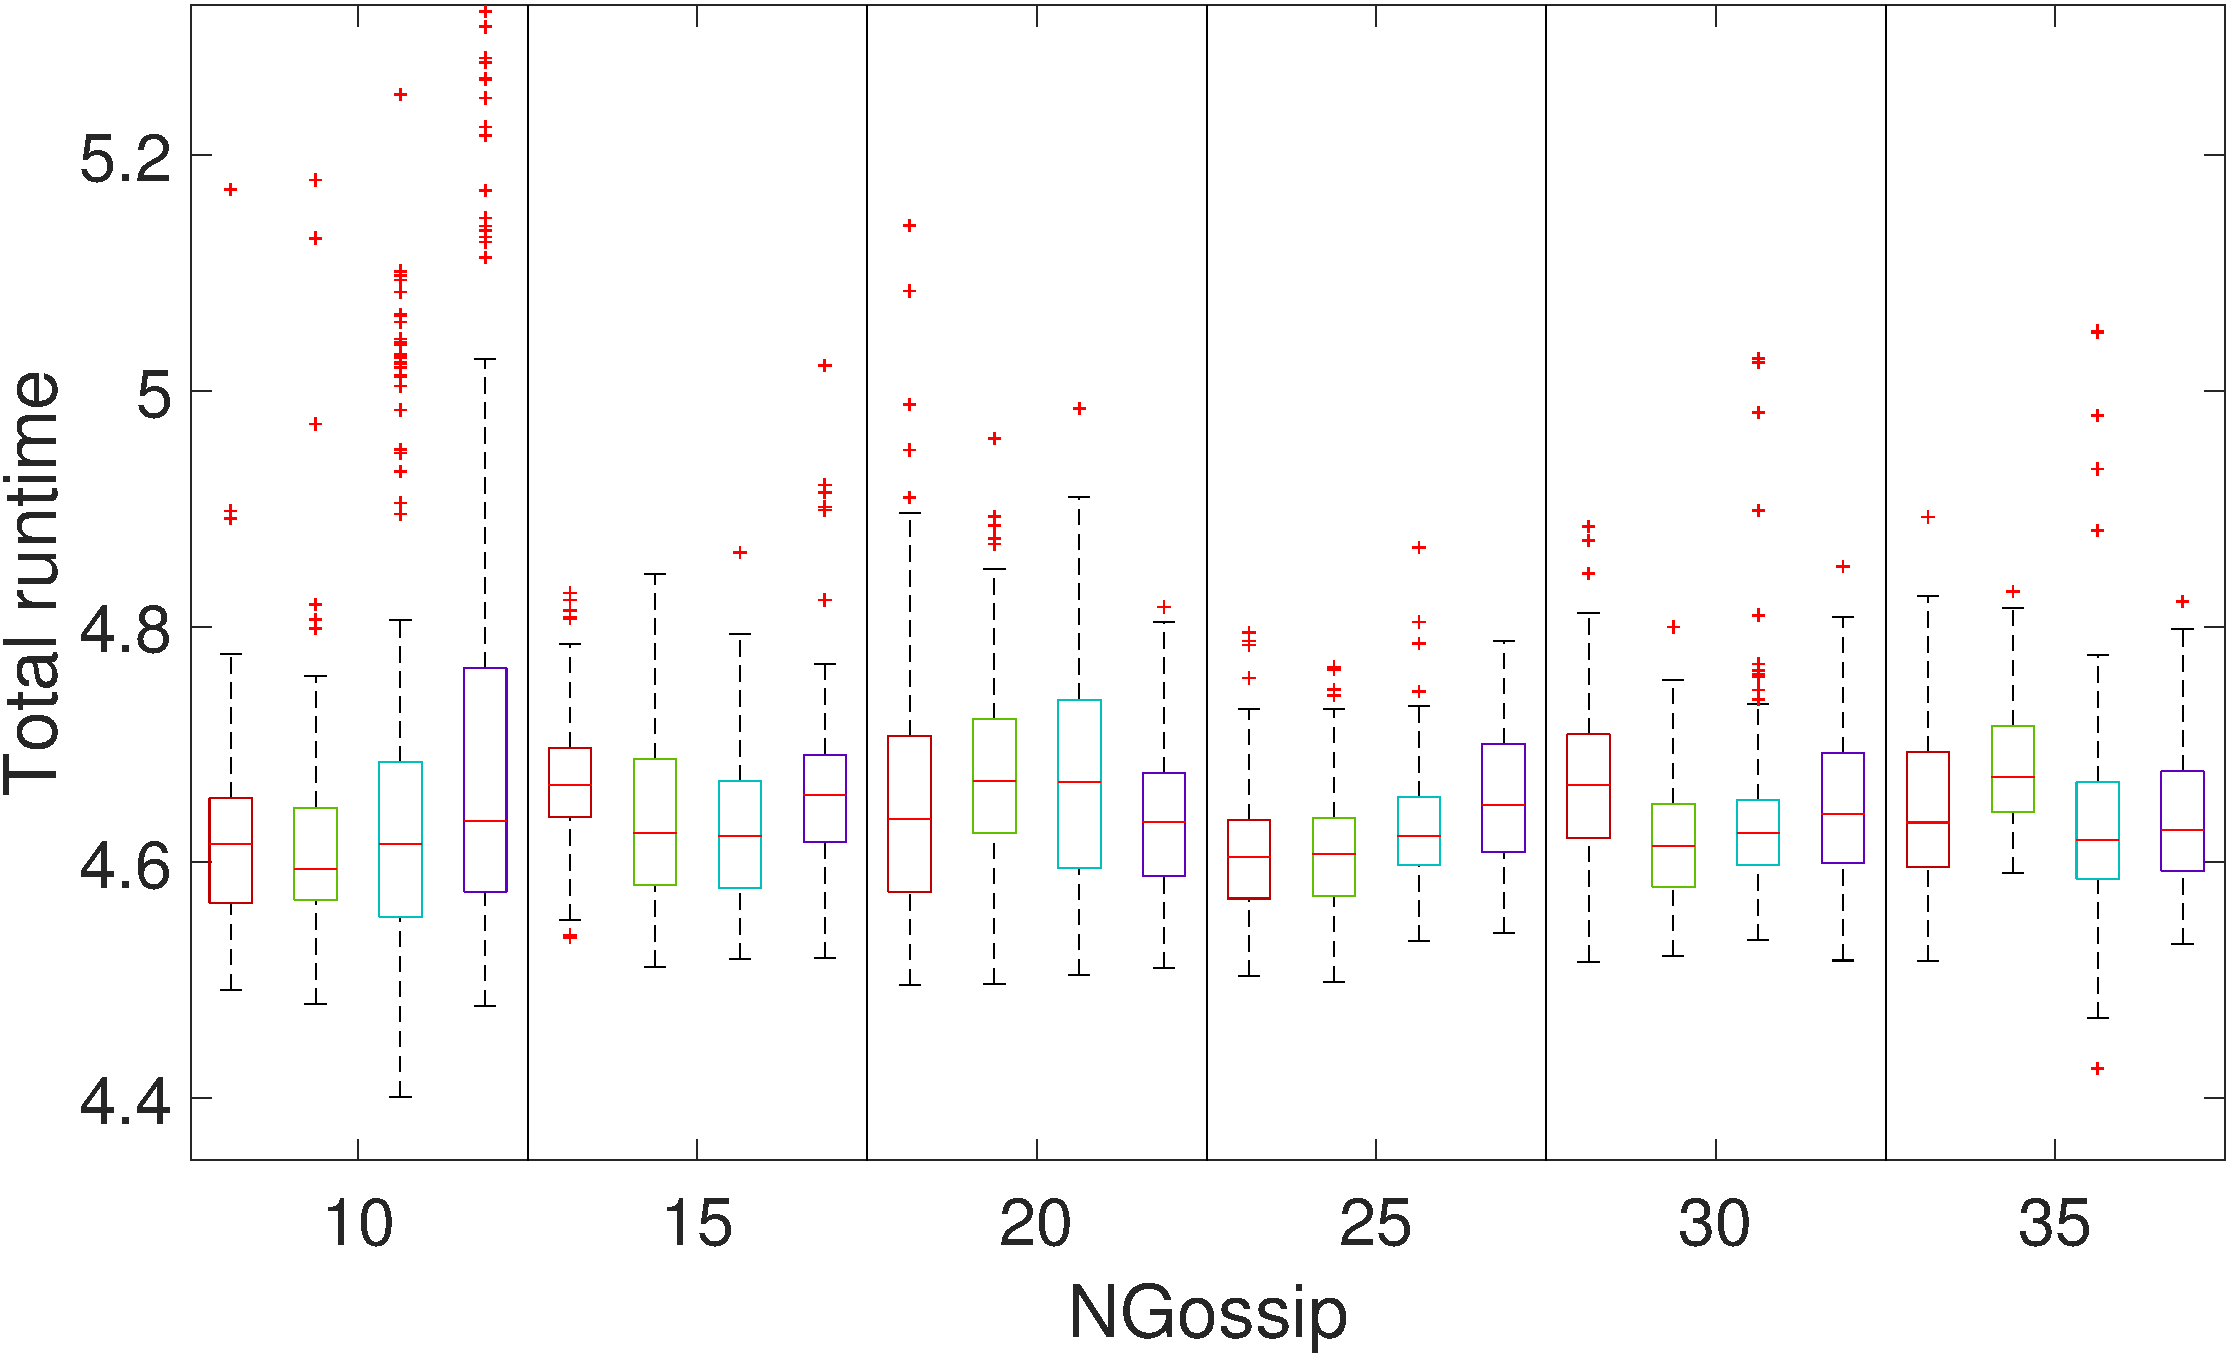
\includegraphics[width=0.65\textwidth]{Figures/boxplot_LApf_time}}
%%\end{subfigure}
%\begin{subfigure}[AER]
%{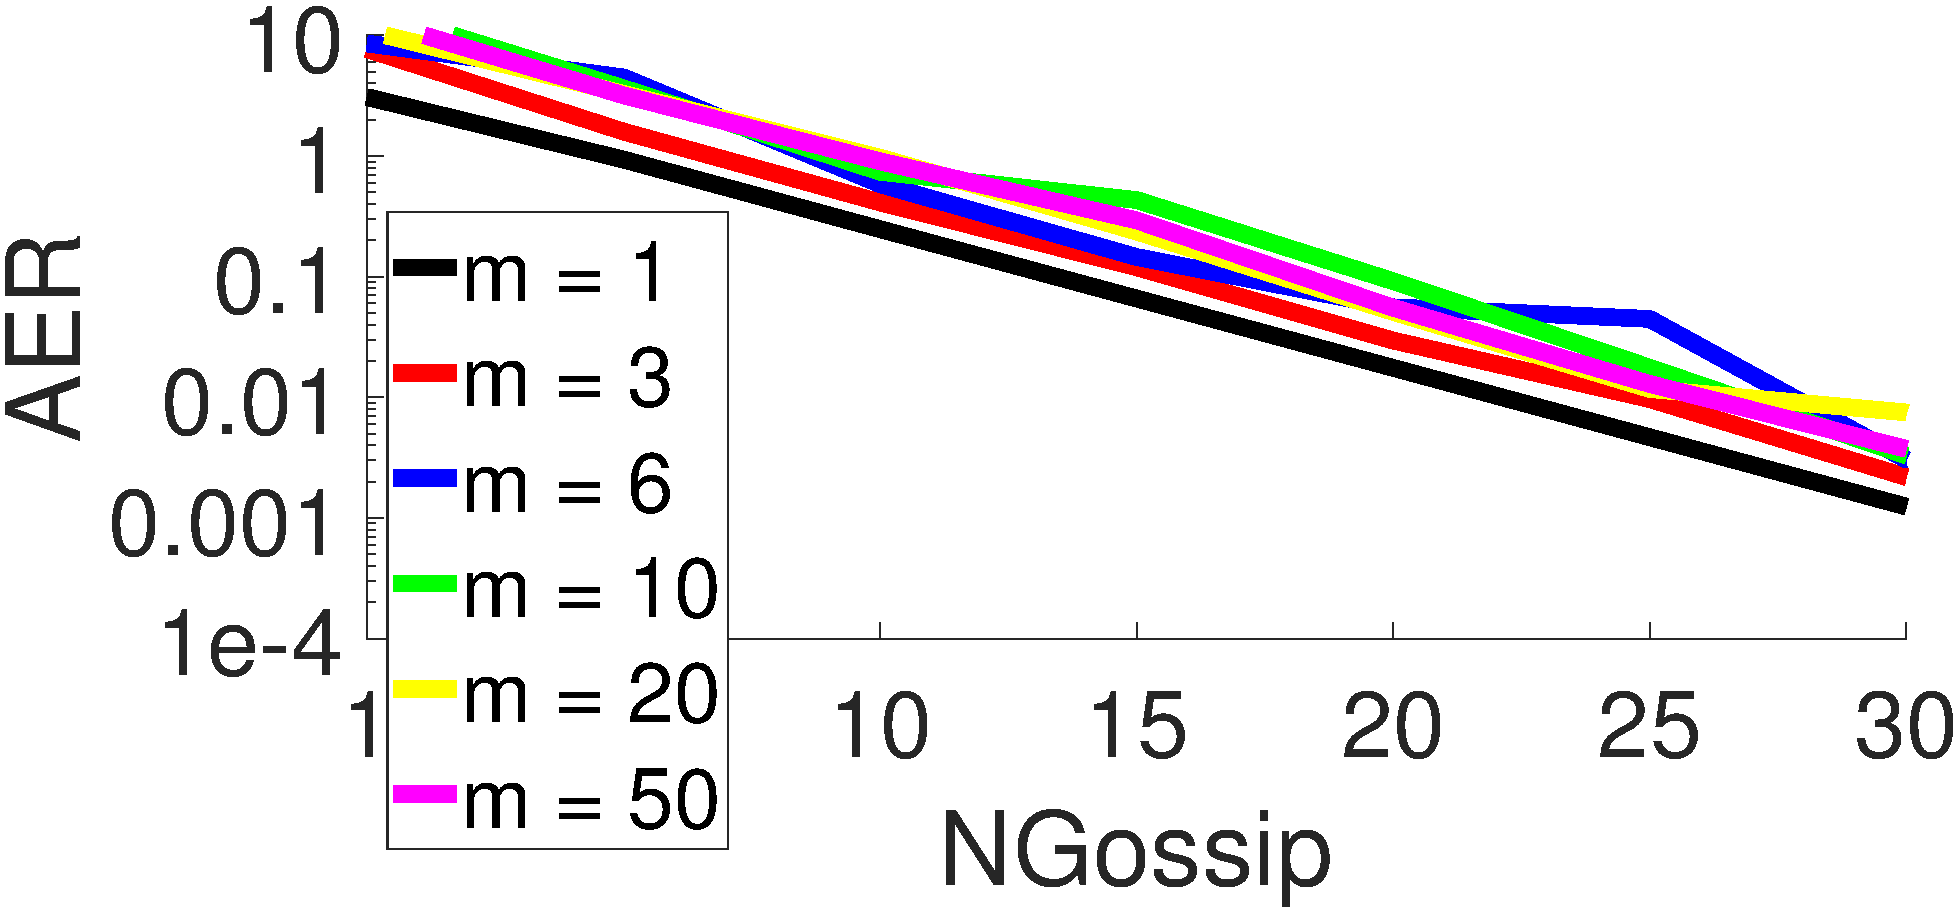
\includegraphics[width=0.47\textwidth]{Figures/curve_LApf_AER}}
%\end{subfigure}
%\caption{RMSE and AER of LApf with respect to $NGossip$ for $N=500$ and different values of $m$. All data points are averaged over 50 time steps and 200 Monte Carlo trials.}
%\label{fig:results_LApf}
%\end{figure}
%
%Consider first RMSE. We do not show the curve for $m=1$ as the filter breaks down and yields an average RMSE over 12. For $m=3$, the RMSE is significantly higher than the other curves. This suggests that a minimum number of eigenvectors is needed to encode particle log-likelihoods without significant information loss. As we increase $m$, the RMSE decreases as expected; although the difference is quite marginal for $m\geq 6$. 
%
%More interestingly, as few as 10 gossip iterations per time step are sufficient to yield robust tracking performance even though the AER of LApf is quite close to that of CSSpf and LCpf for the same $NGossip$ and $N$. This would suggest that LApf is much more robust to gossiping error. 
%
%%To confirm our conjecture regarding the choice of $m$, we again compute $||W_{\text{true}}-_{\text{approx}}||_2$ with respect to $m$ and show the results in Fig.~\ref{fig:boxplot_LApf_weight_discrepancy}. The error is highest at $m=1$ (by almost a factor of 10). At $m=6$, the average discrepancy is as low as $4e-4$. Increasing $m$ to 100 only reduces the error by a factor of 3 while increasing the communication overhead by a factor of 15.  
%%
%%\begin{figure}
%%\centering
%%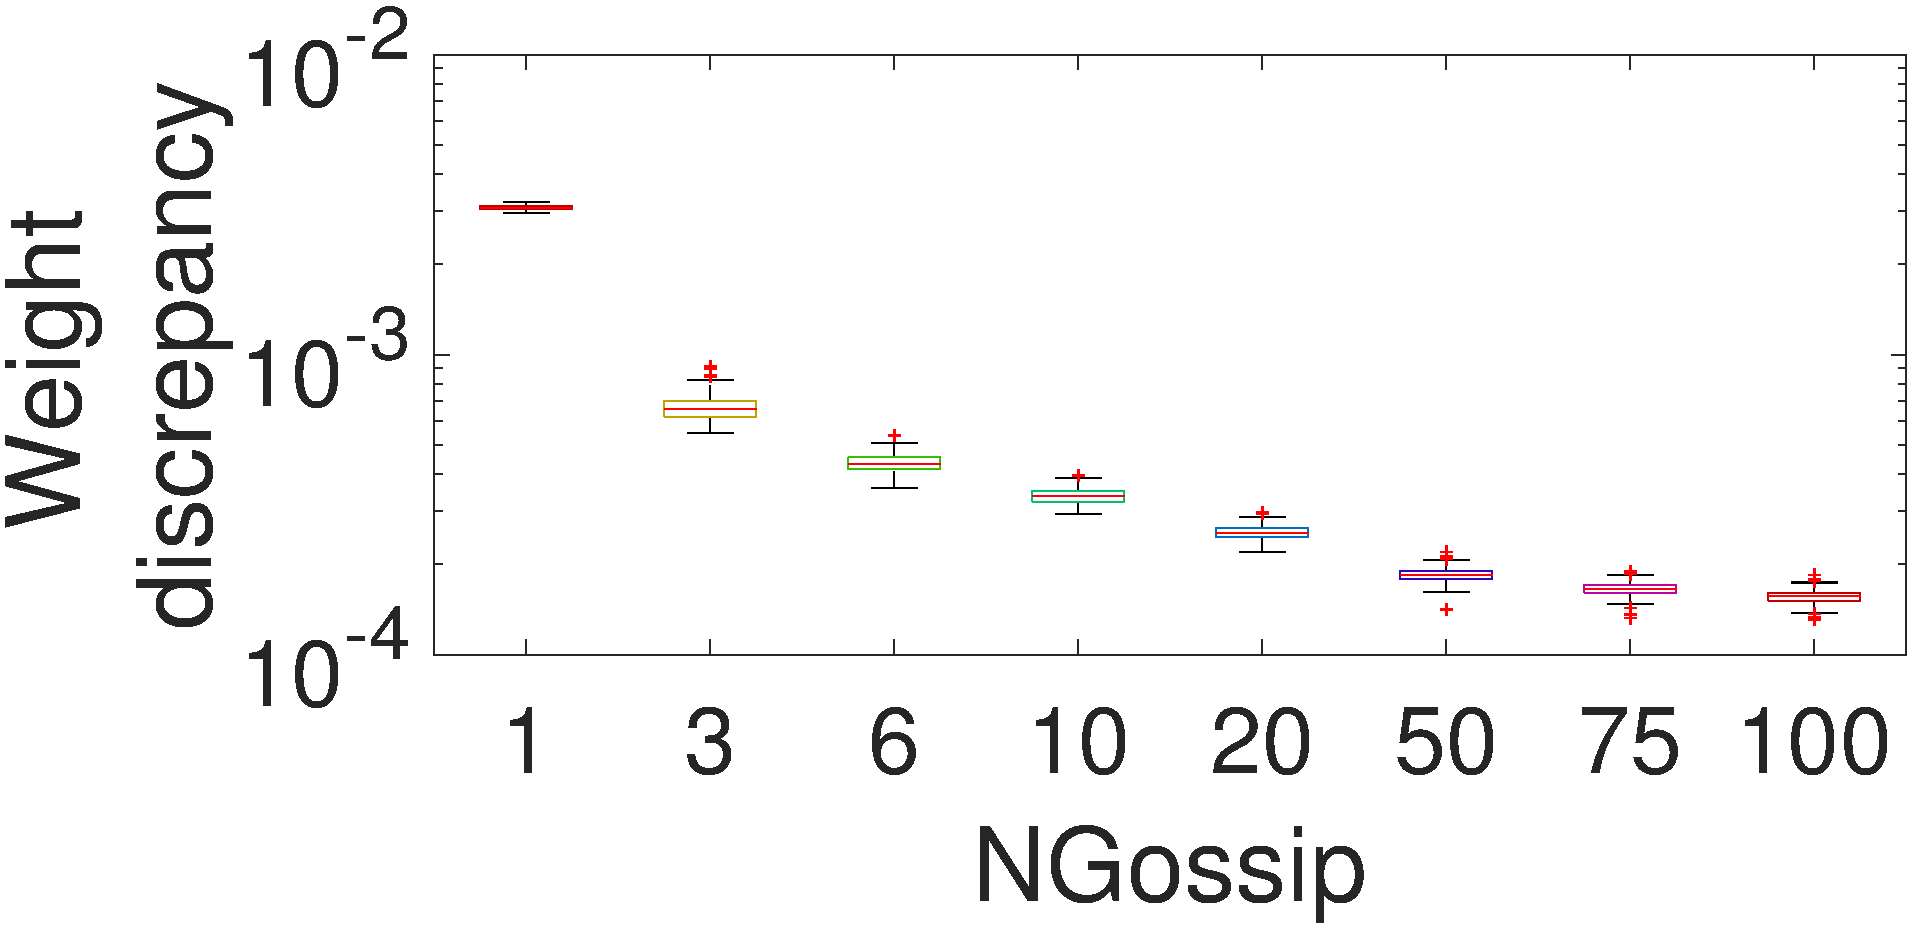
\includegraphics[width=0.6\textwidth]{Figures/boxplot_LApf_weight_discrepancy}
%%\caption{Boxplot of weight discrepancy with respect to $m$}
%%\label{fig:boxplot_LApf_weight_discrepancy}
%%\end{figure}
%
%
%\subsection{Cluster particle filter}
%%The number of clusters $C$ offers a trade-off between tracking performance and computational/communication overhead. Higher number of clusters should yield better performance albeit at higher overhead. In fact, it is clear that the parameter $C$ is analogous to $m$ in LApf. Fig.~\ref{fig:results_Clusterpf} shows the tracking results. 
%
%\begin{figure}
%\centering
%\begin{subfigure}[RMSE]
%{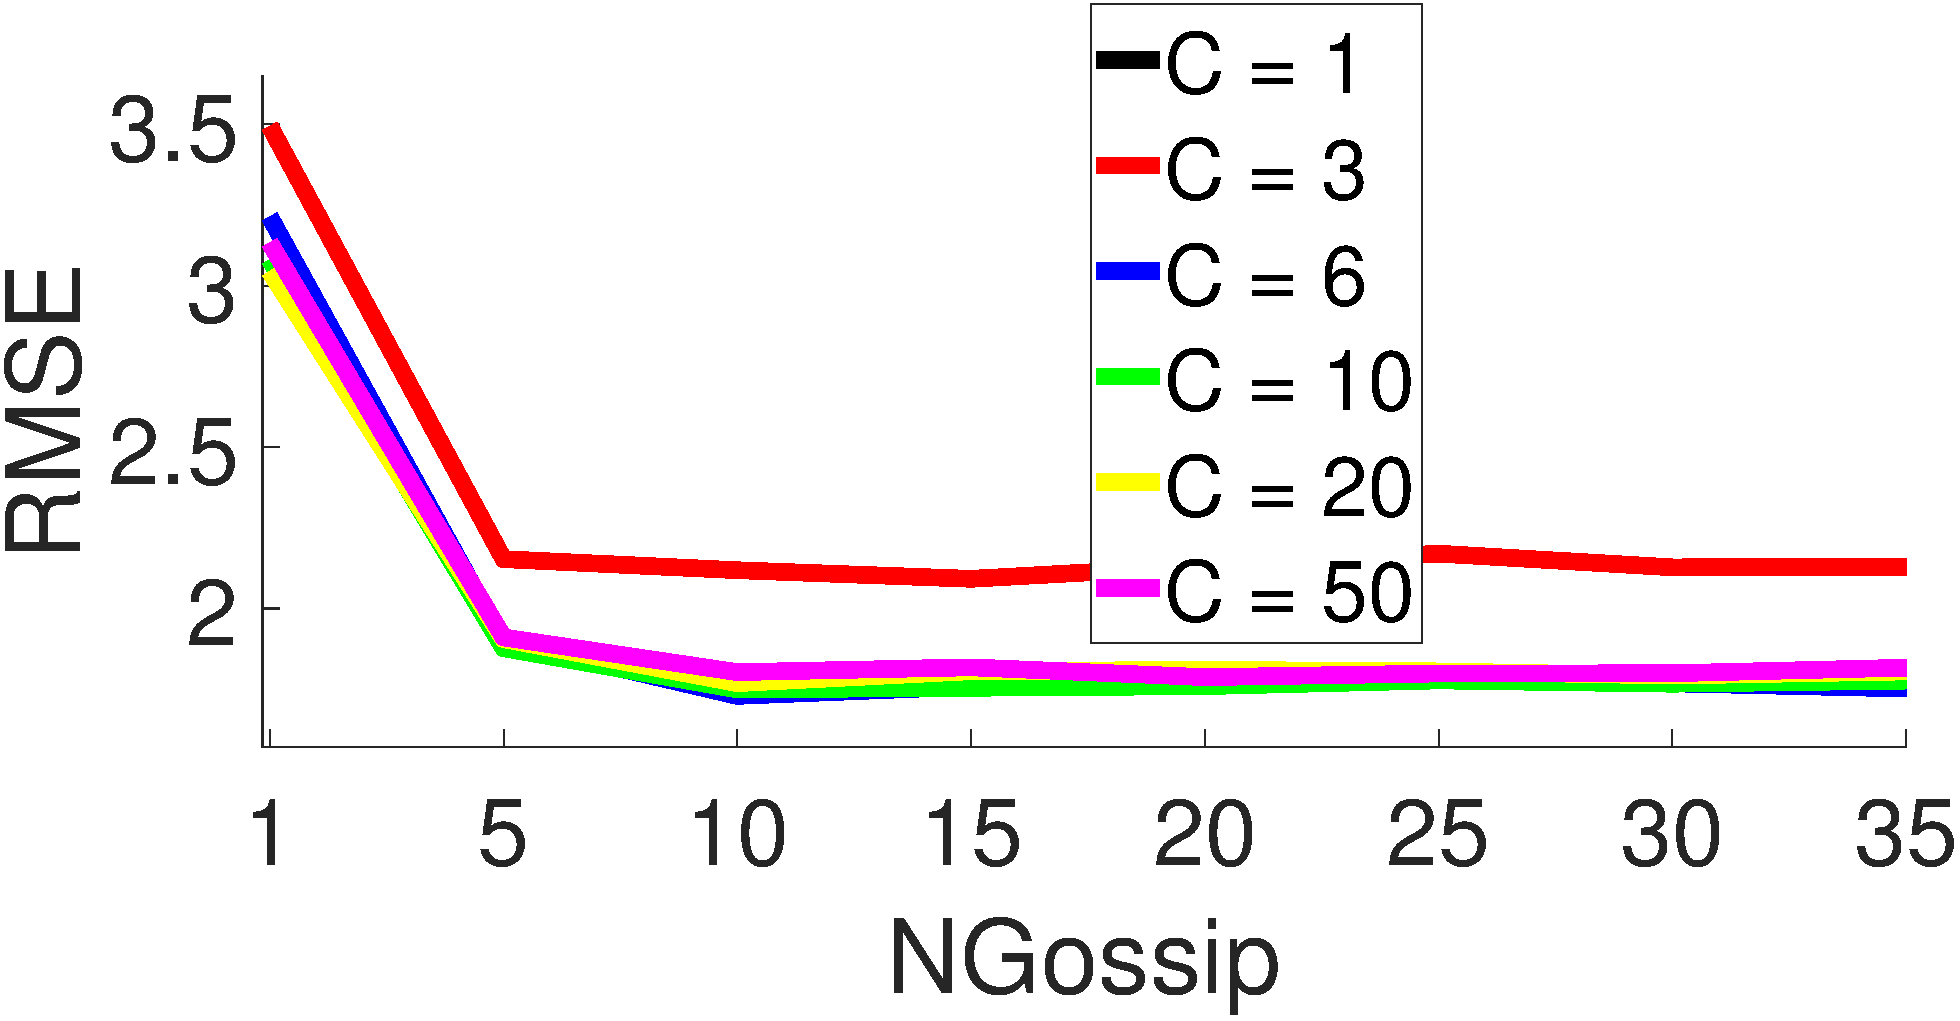
\includegraphics[width=0.49\textwidth]{Figures/curve_Clusterpf_RMSE}}
%\end{subfigure}
%%\begin{subfigure}[total runtime]
%%{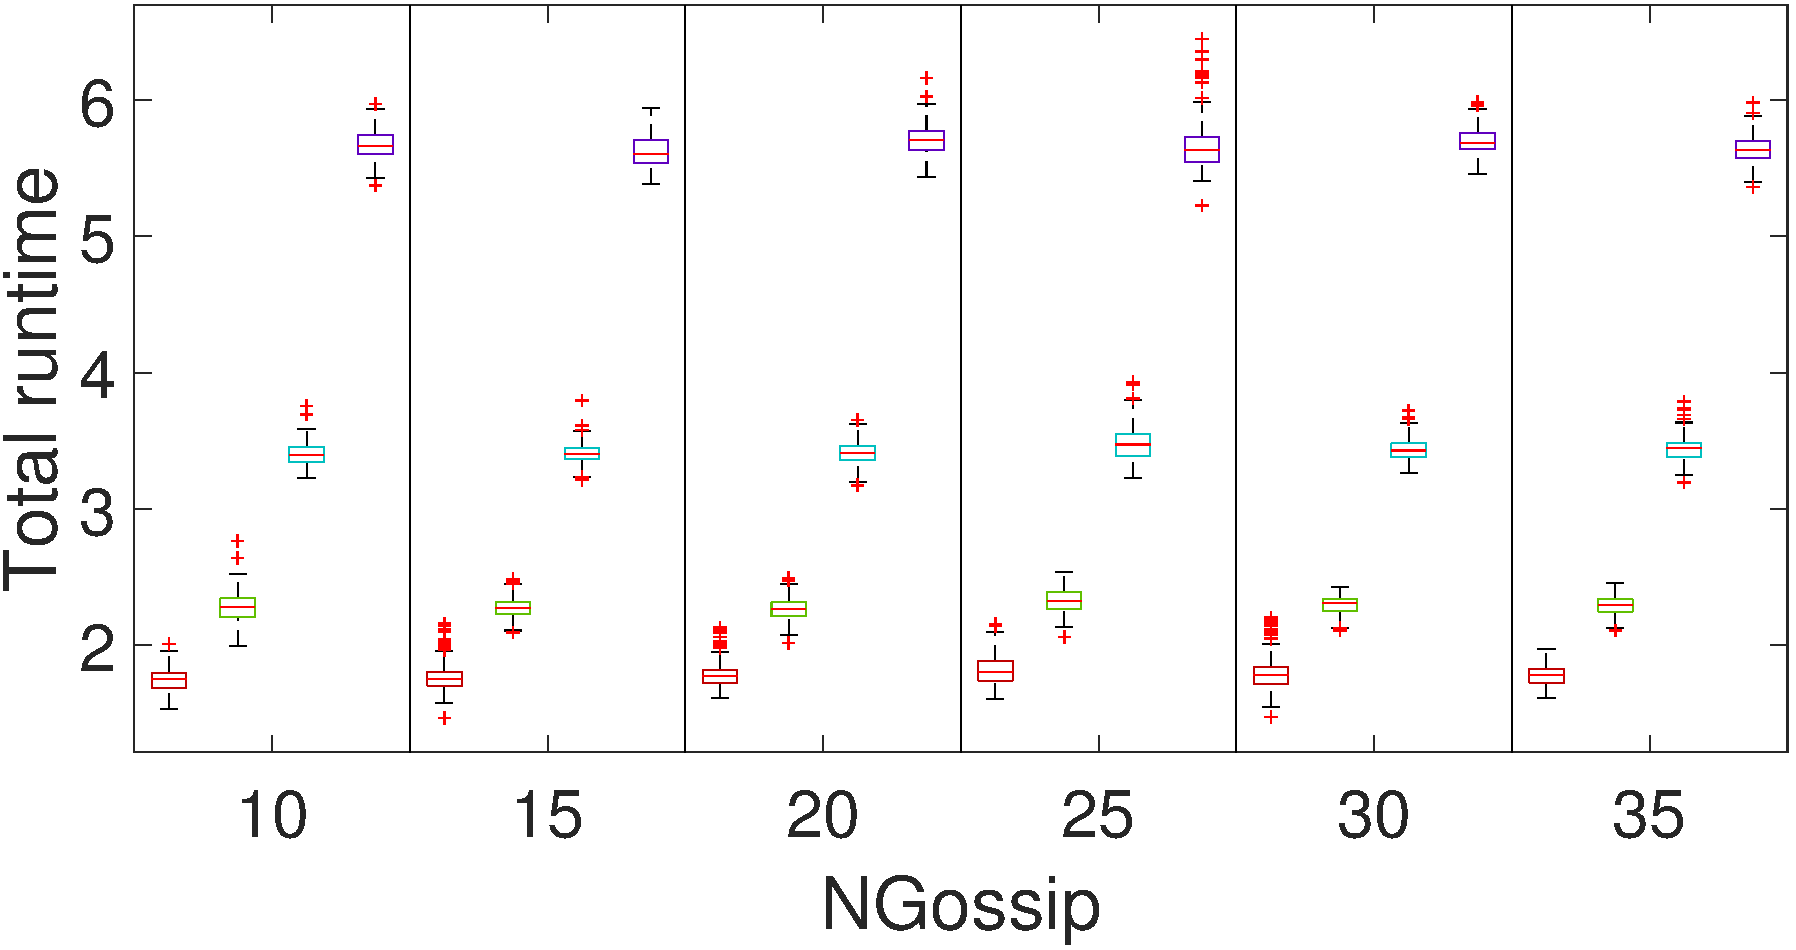
\includegraphics[width=0.65\textwidth]{Figures/boxplot_Clusterpf_time}}
%%\end{subfigure}
%\begin{subfigure}[AER]
%{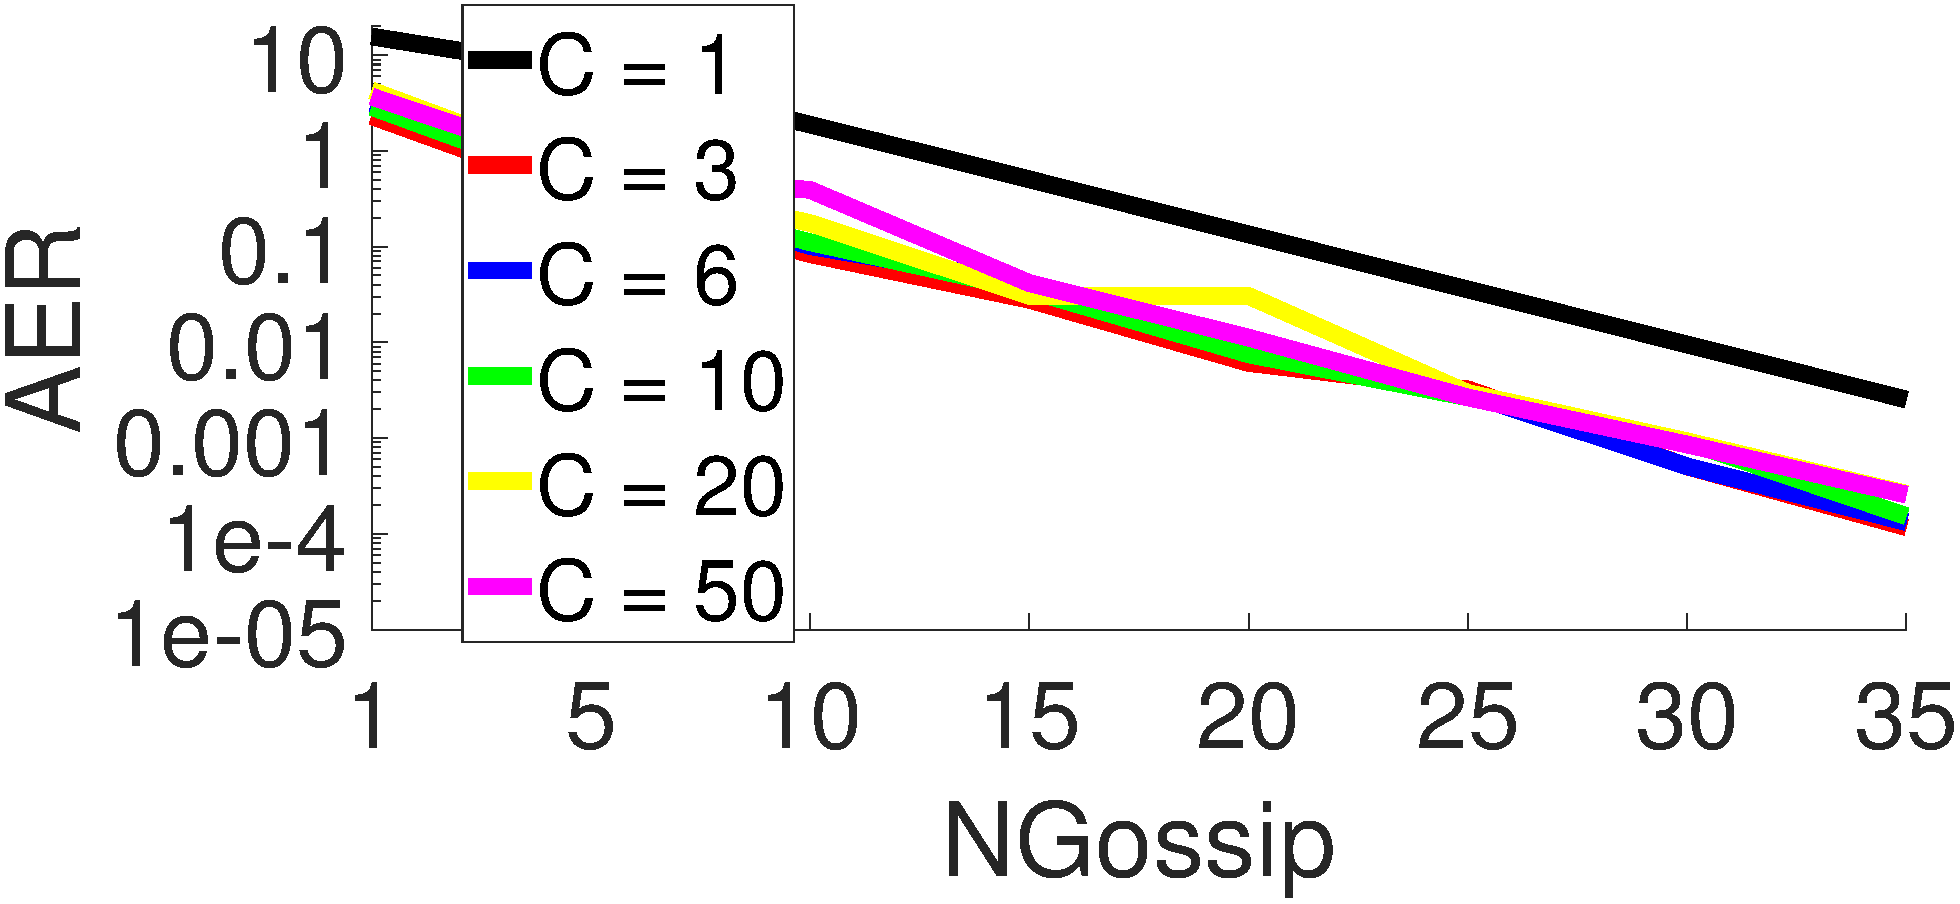
\includegraphics[width=0.49\textwidth]{Figures/curve_Clusterpf_AER}}
%\end{subfigure}
%\caption{RMSE and AER of Clusterpf with respect to $NGossip$ for $N=500$ and different values of $C$. All data points are averaged over 50 time steps and 200 Monte Carlo trials.}
%\label{fig:results_Clusterpf}
%\end{figure}
%
%%\begin{figure}
%%\centering
%%%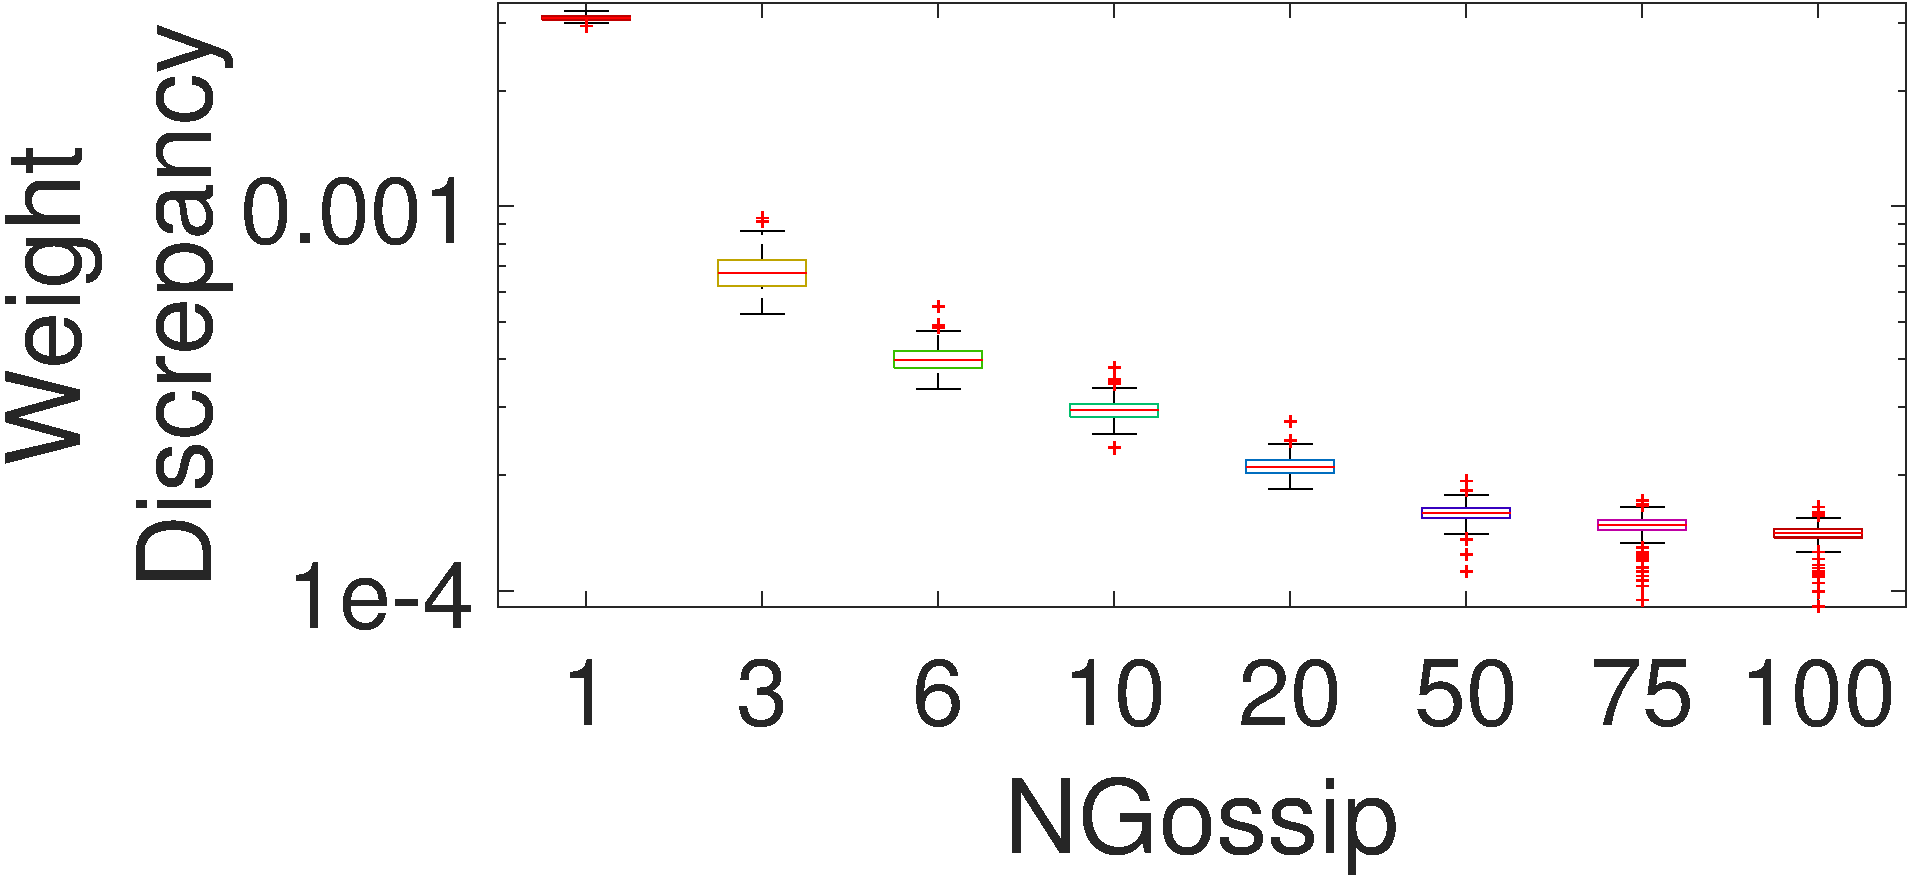
\includegraphics[width=0.6\textwidth]{Figures/boxplot_Clusterpf_weight_discrepancy}
%%%\caption{Boxplot of weight discrepancy with respect to $C$}
%%%\label{fig:boxplot_Clusterpf_weight_discrepancy}
%%%\end{figure}
%%
%%Again, we omit the curve for $C=1$ as the filter breaks down and yields an RMSE above 12. For $C\geq 5$, the RMSE is quite consistent for $NGossip \geq 6$. As in the case of LApf, Clusterpf is quite robust to gossiping error and yields good performance for $NGossip \geq 5$. 
%%
%%%As in the case of LApf, we compute and report the average weight discrepancy in Fig.~\ref{fig:boxplot_Clusterpf_weight_discrepancy}. The discrepancy is highest at $C=1$ as expected. Increasing $C$ from 6 to 75 decreases the approximation error by no more than half at the cost of a tenfold increase in communication overhead. 
%%
%
%
%
\subsection{Performance comparison between filters}
In this section, we compare the four filters against each other. We use a centralized bootstrap particle filter as baseline. Finally, we include a modified version of LCpf where we use the Gram-Schmidt process to obtain an orthonormal encoding matrix $\Phi'$ (i.e., $||\Phi'(:,i)||_2=1,i=1,...J$). This filter is referred to as LCpf-GS. We consider three different test tracks shown in Fig.~\ref{fig:test_tracks}. 

\begin{figure}
\centering
\begin{subfigure}[Track 1]
{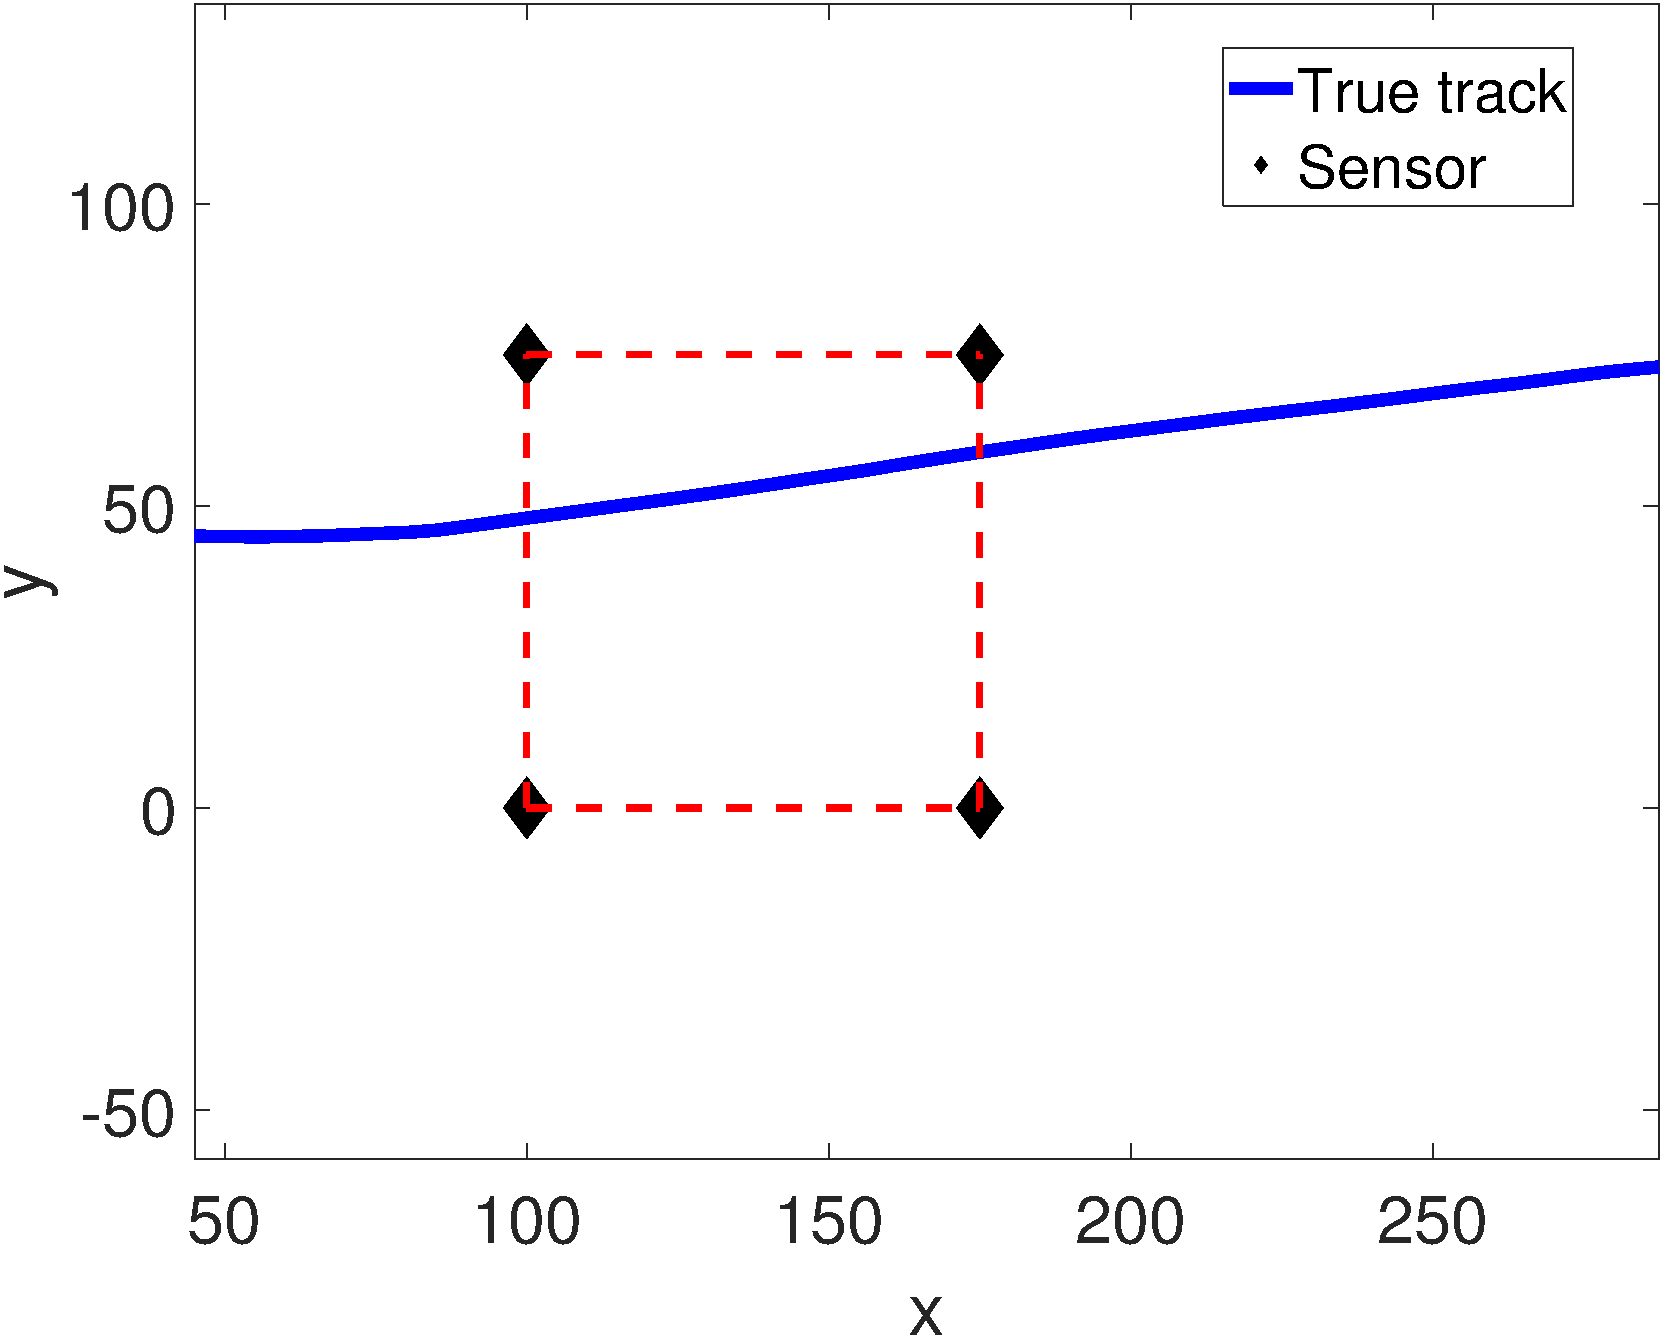
\includegraphics[width=0.32\textwidth]{Figures/track1}}
\end{subfigure}
\begin{subfigure}[Track 2]
{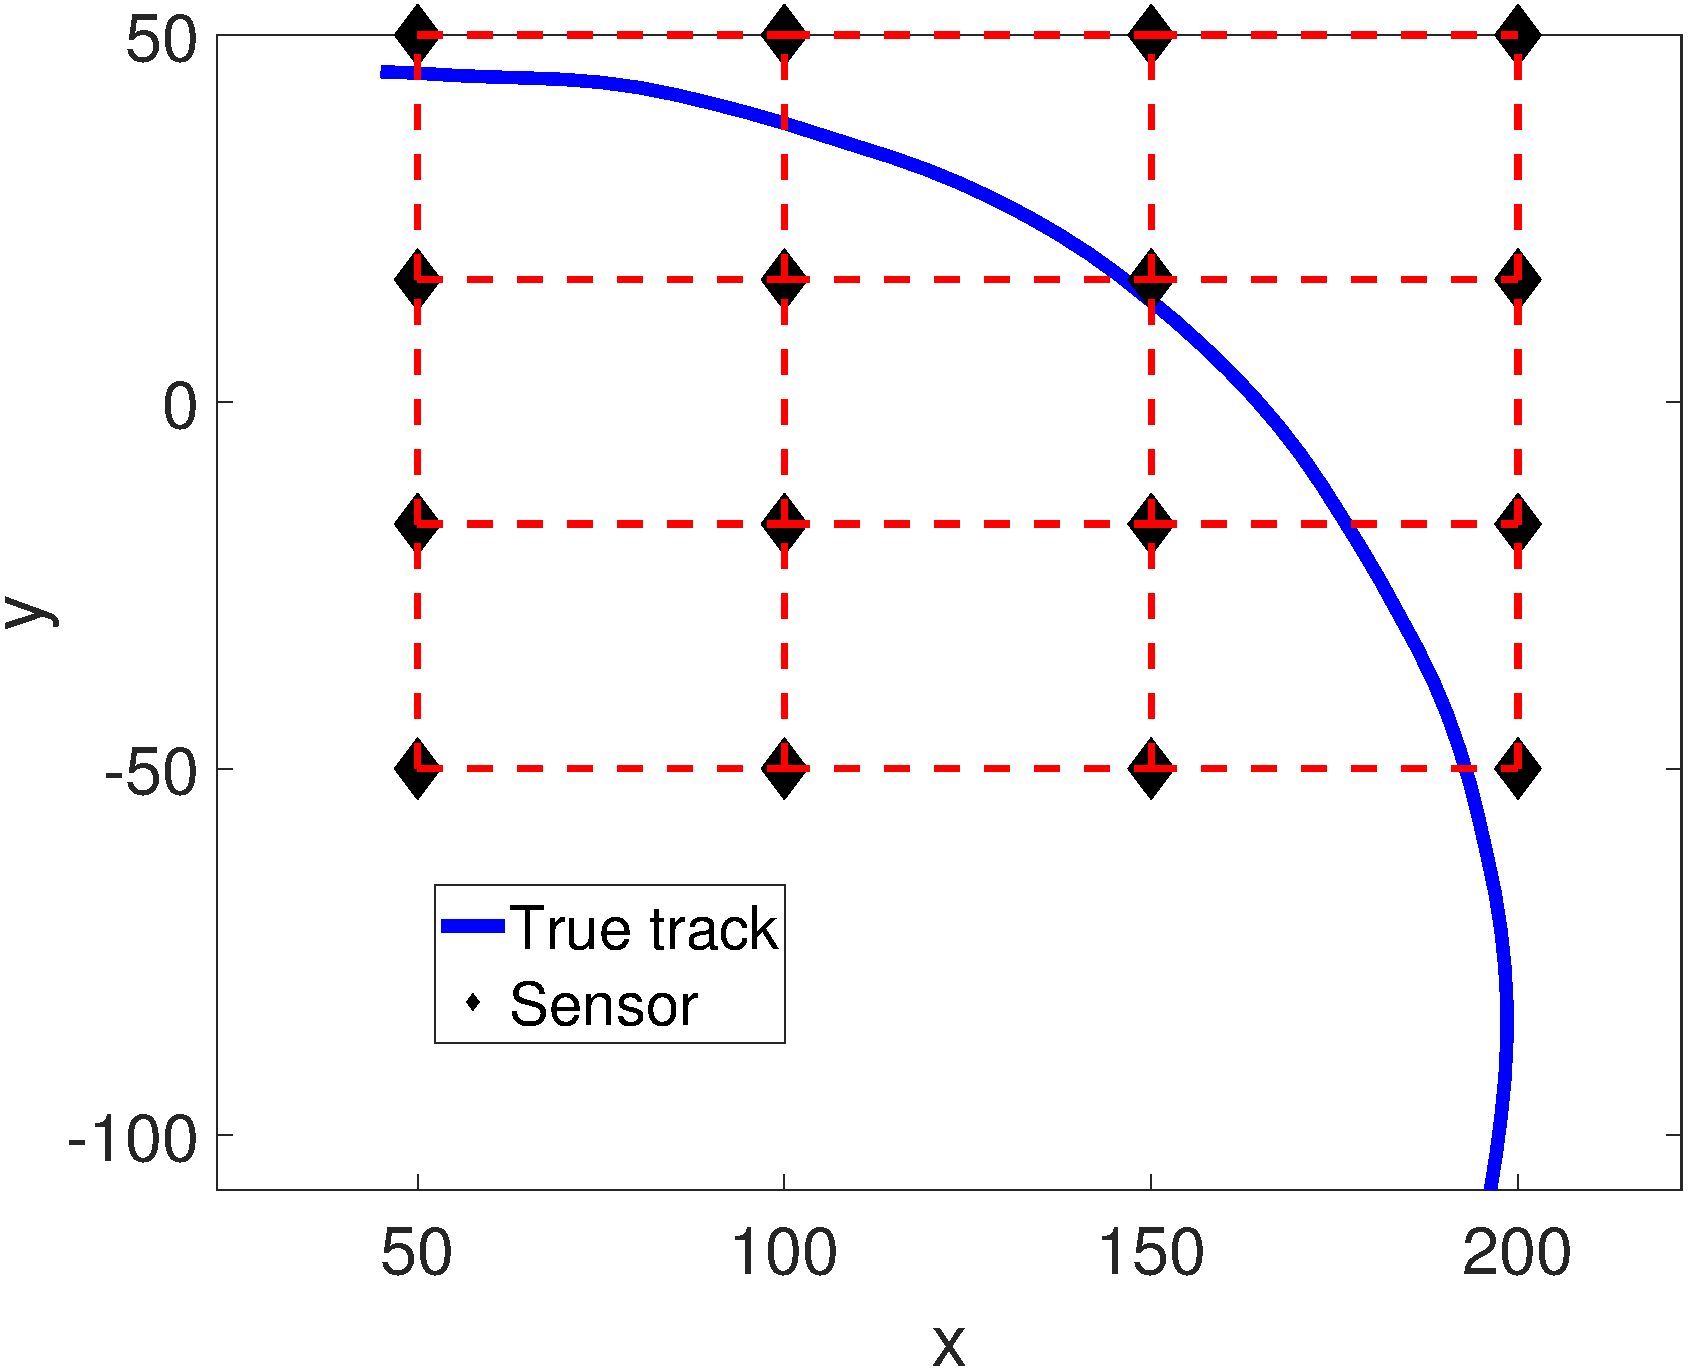
\includegraphics[width=0.32\textwidth]{Figures/track2}}
\end{subfigure}
\begin{subfigure}[Track 3]
{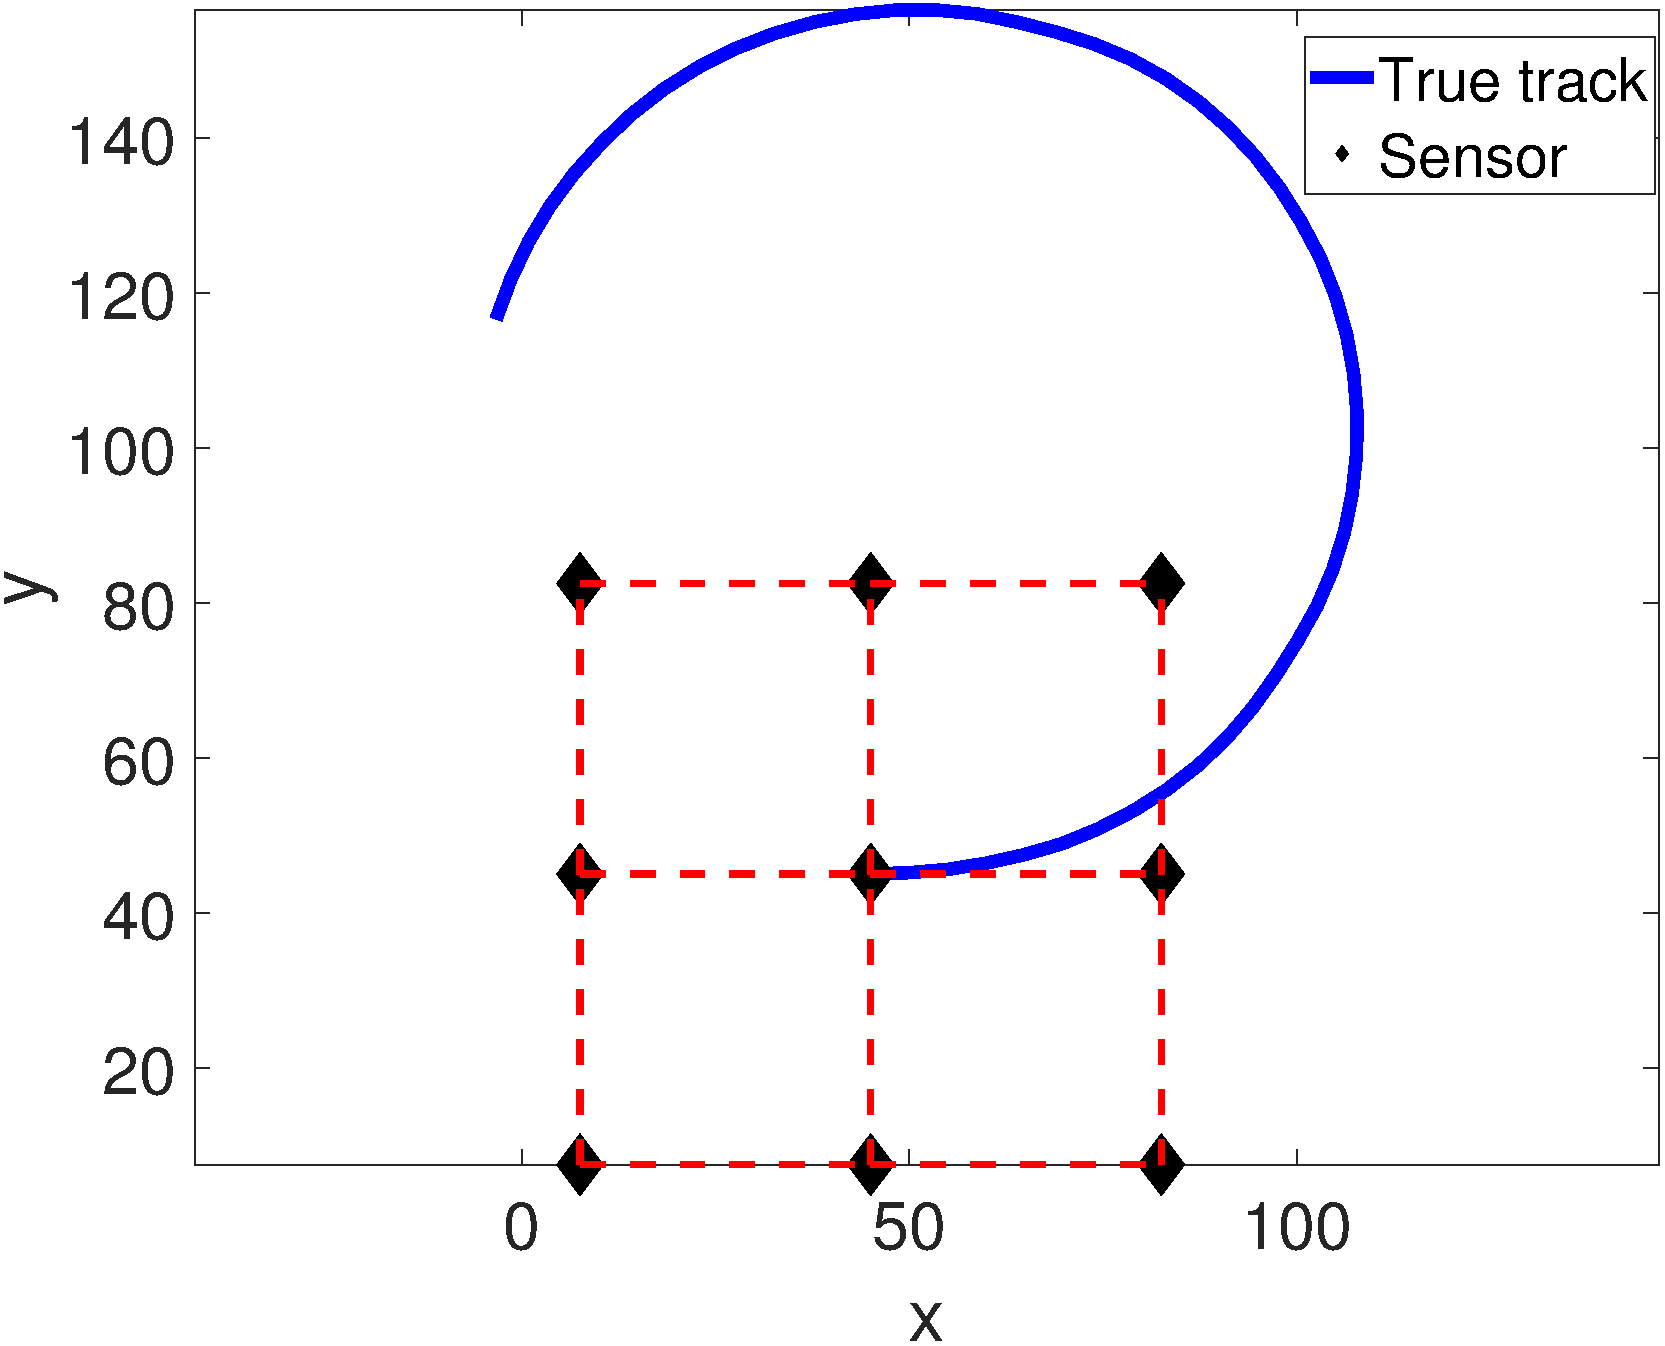
\includegraphics[width=0.32\textwidth]{Figures/track3}}
\end{subfigure}
\caption{Target tracks (blue curve) and sensor positions (black diamond). Sensors connected by red dashed lines are within broadcast range of each other.}
\label{fig:test_tracks}
\end{figure}

\begin{figure}
\centering
\begin{subfigure}[RMSE]
{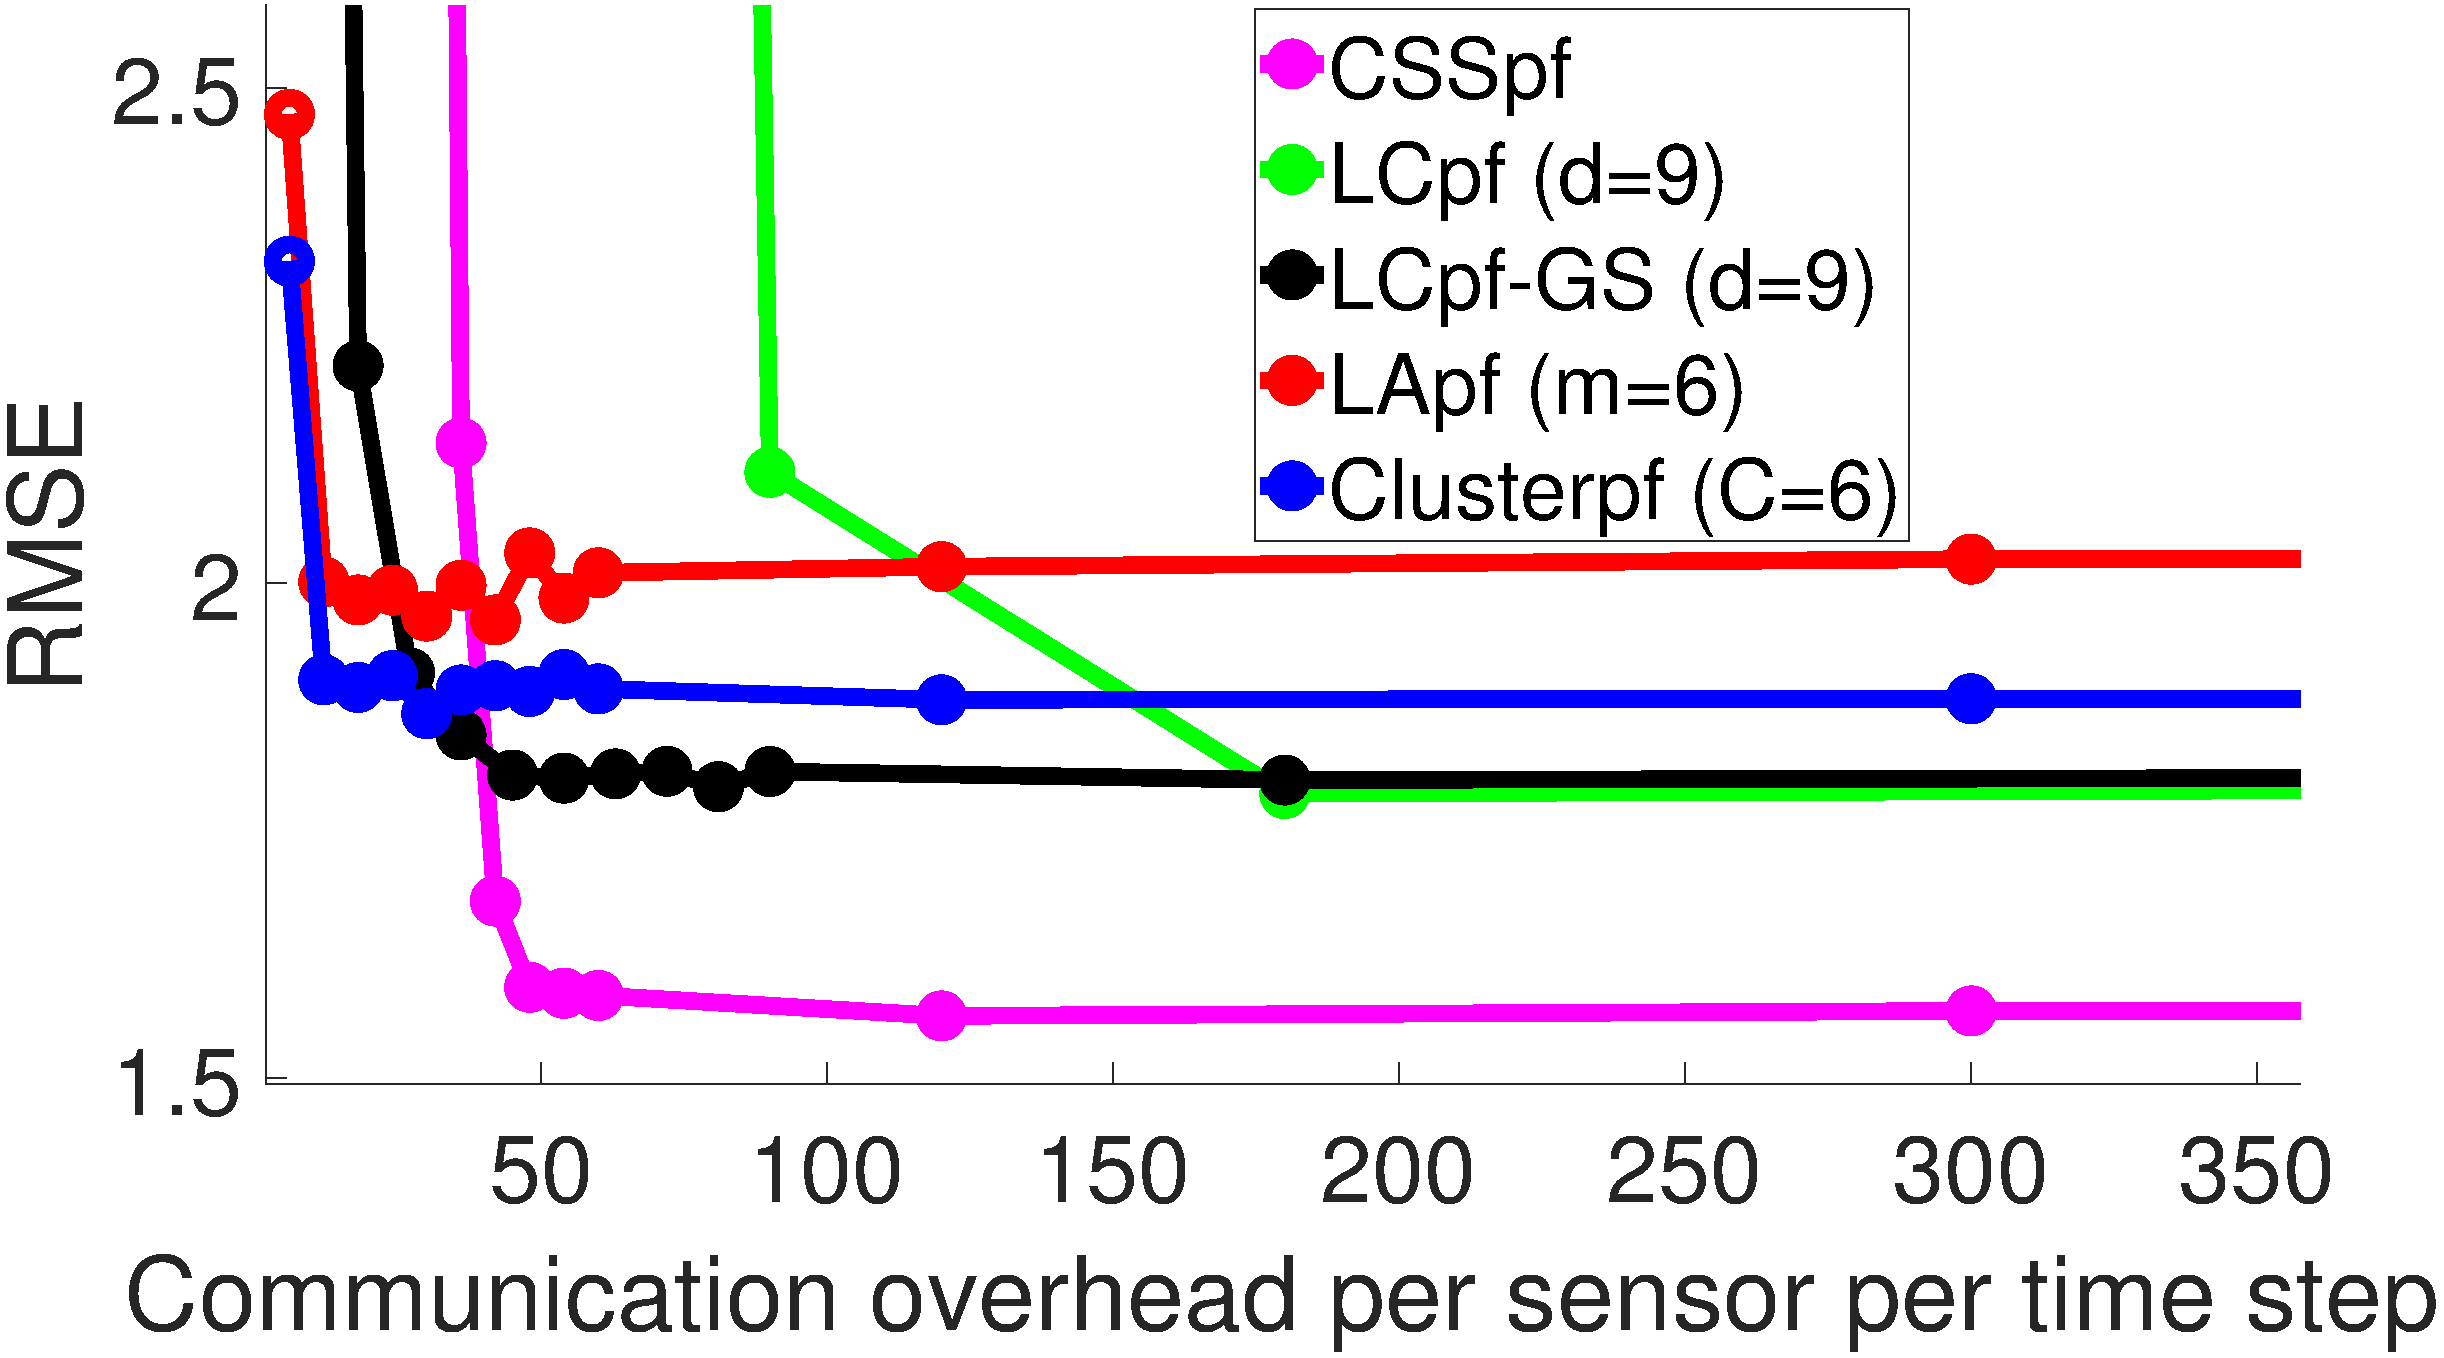
\includegraphics[width=0.49\textwidth]{Figures/Track1_bearing_RMSE}}
\end{subfigure}
\begin{subfigure}[RMSE]
{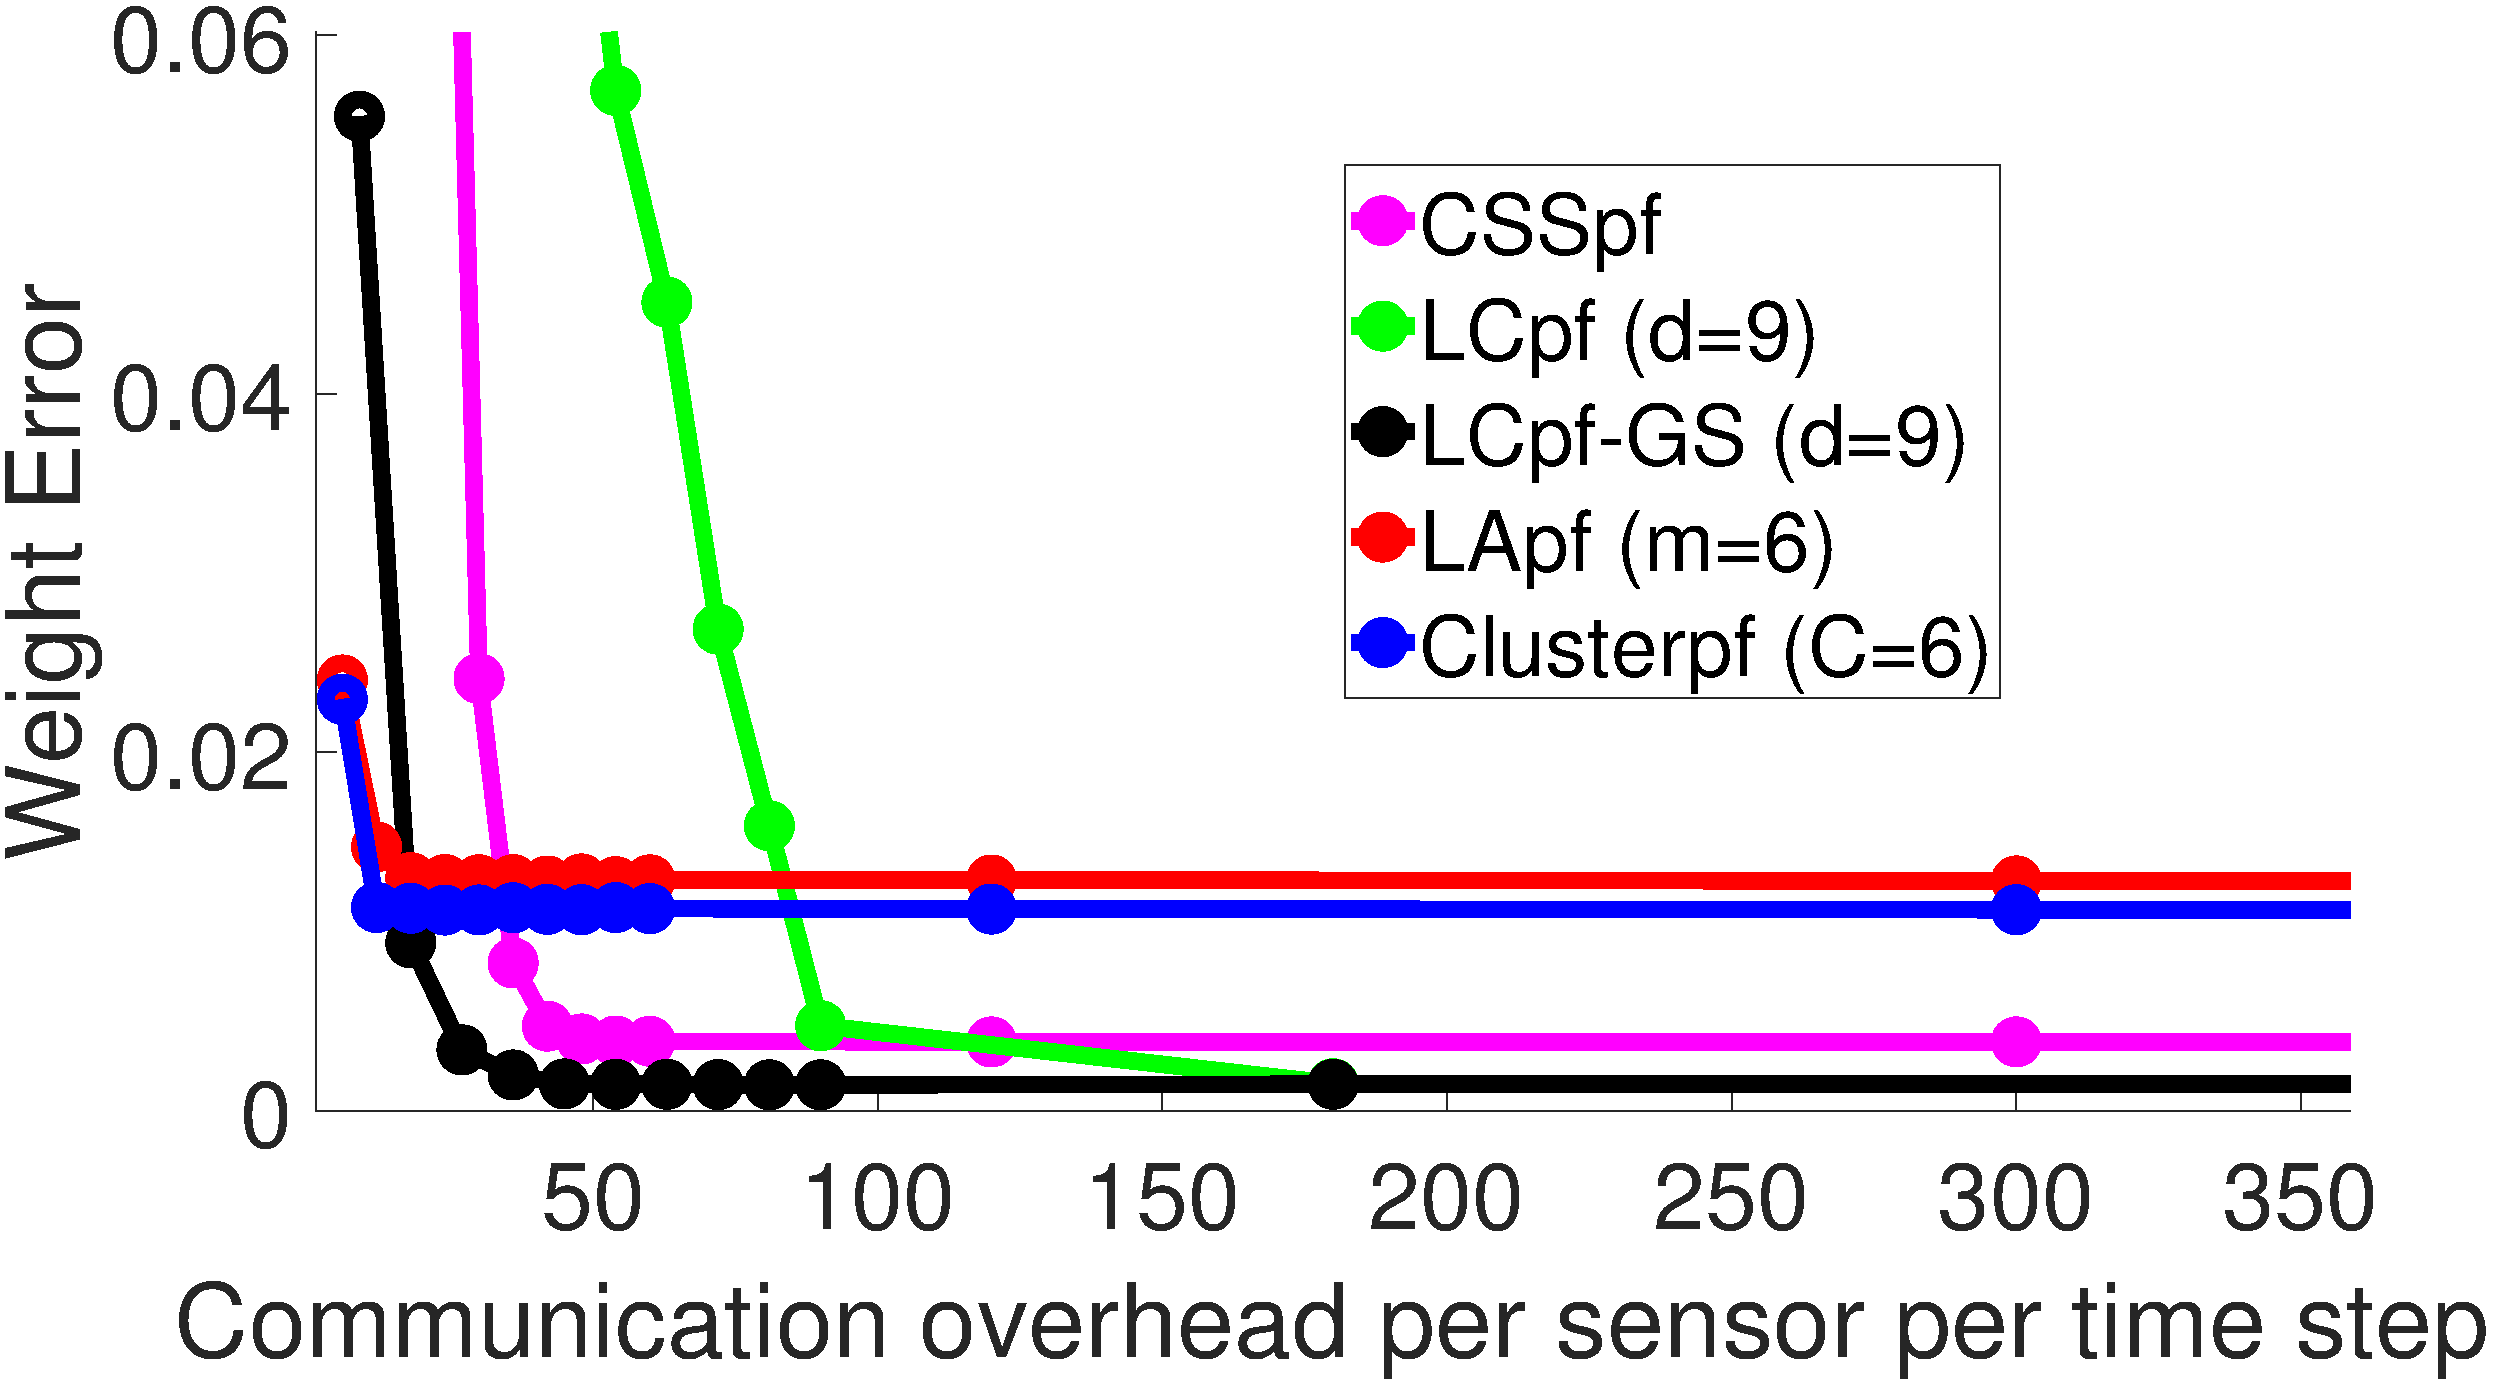
\includegraphics[width=0.49\textwidth]{Figures/Track1_bearing_WError}}
\end{subfigure}
\caption{Average RMSE and particle weights error with respect to total communication overhead per time step for track 1 ($N=500$, 200 Monte Carlo trials).}
\label{fig:Track1_results}
\end{figure}

%For CSSpf and LCpf, we vary only the number of gossip iterations per time step. We run two variations of LApf and Clusterpf. In the first version, we fix $m$ and $C$, the number of scalars to aggregate per time step, and increase $NGossip$. In the second version, we fix $NGossip$ and increase $m$ and $C$ accordingly. 

Fig.~\ref{fig:Track1_results} shows the average RMSE and weight error with respect to communication overhead per sensor per time step for all algorithms for track 1. For overhead $< 25$, Clusterpf and LApf have the lowest RMSE. Note that these two filters have low RMSE even at $NGossip=1$ (i.e., communication overhead = 1*6 = 6). For overhead $> 50$, CSSpf has the best performance by a significant margin. The LCpf requires the highest communication overhead to achieve adequate tracking performance. Consider next the weight error curves. For all filters, we can notice a correspondence between weight error and RMSE (i.e., higher error equals higher RMSE) as expected; but two filters having the same weight error do not necessarily have the same RMSE. For instance, for overhead = 100, LCpf has low weight error on-par with that of CSSpf, yet its RMSE is significantly higher. 

Fig.~\ref{fig:Track2_results} shows the tracking results for track 2. For overhead $< 200$, LApf and Clusterpf have the lowest RMSE. The LCpf-GS achieves similar RMSE as LAPf once the overhead exceeds 200. For LCpf, over 100 Gossip iterations are required to achieve adequate tracking performance. Again, for each filter, there is a clear correspondence between RMSE and weight error. 

\begin{figure}
\centering
\begin{subfigure}[RMSE]
{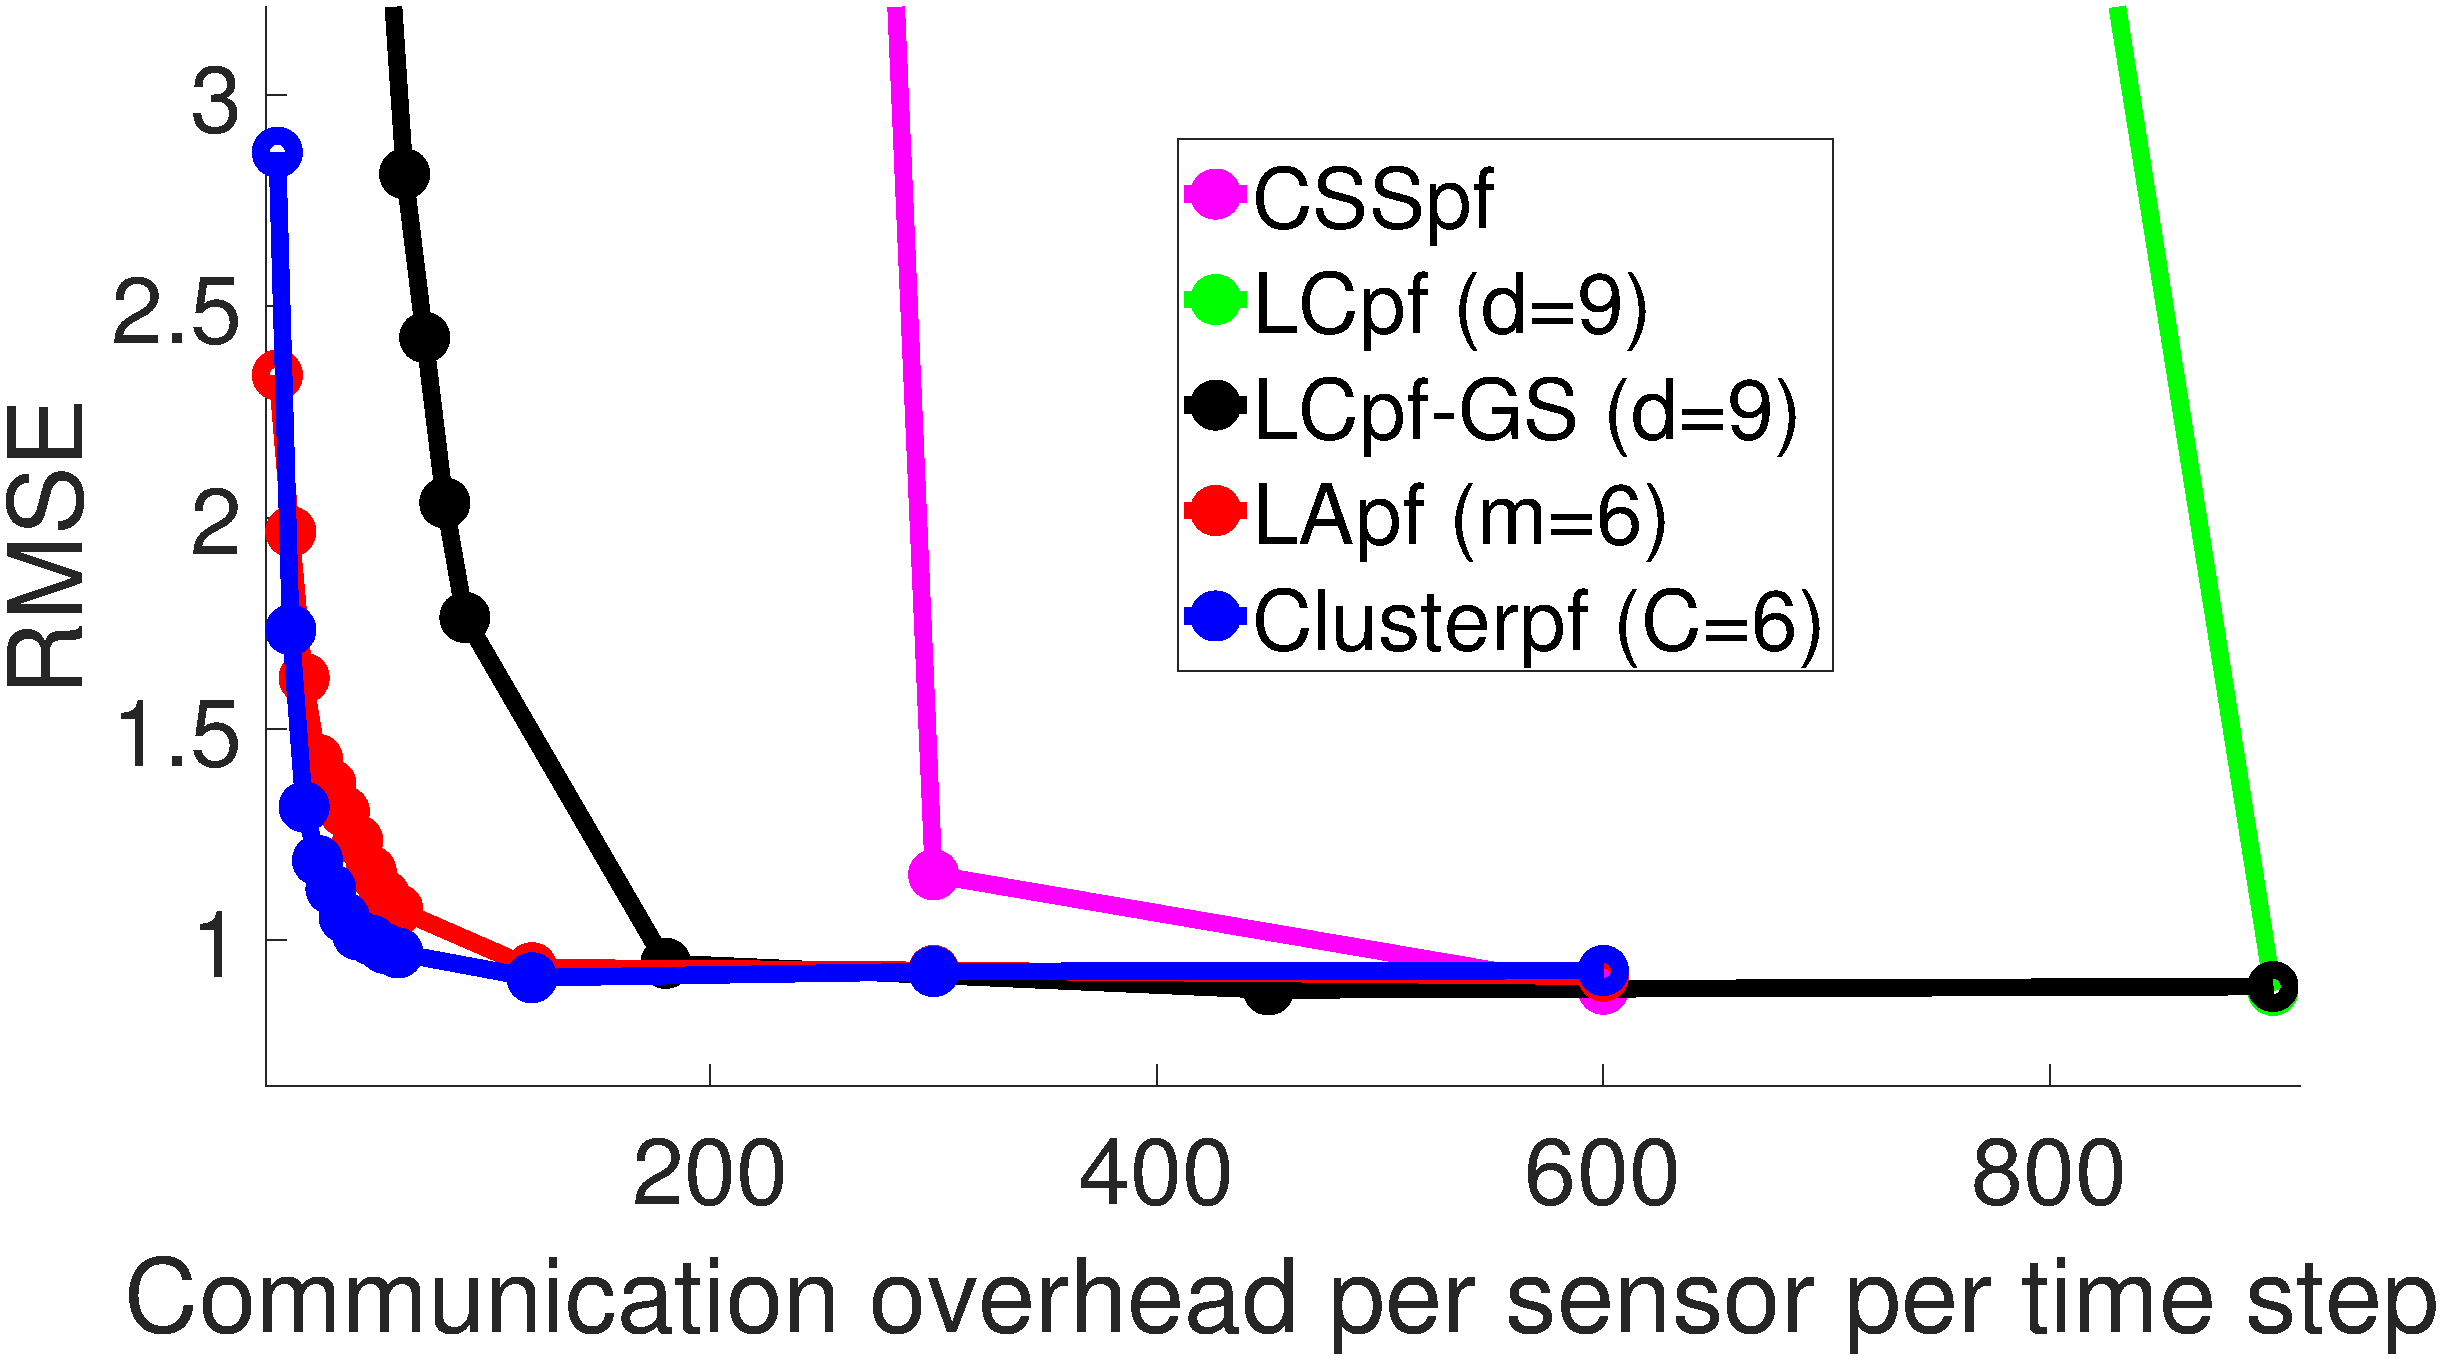
\includegraphics[width=0.49\textwidth]{Figures/Track2_bearing_RMSE}}
\end{subfigure}
\begin{subfigure}[RMSE]
{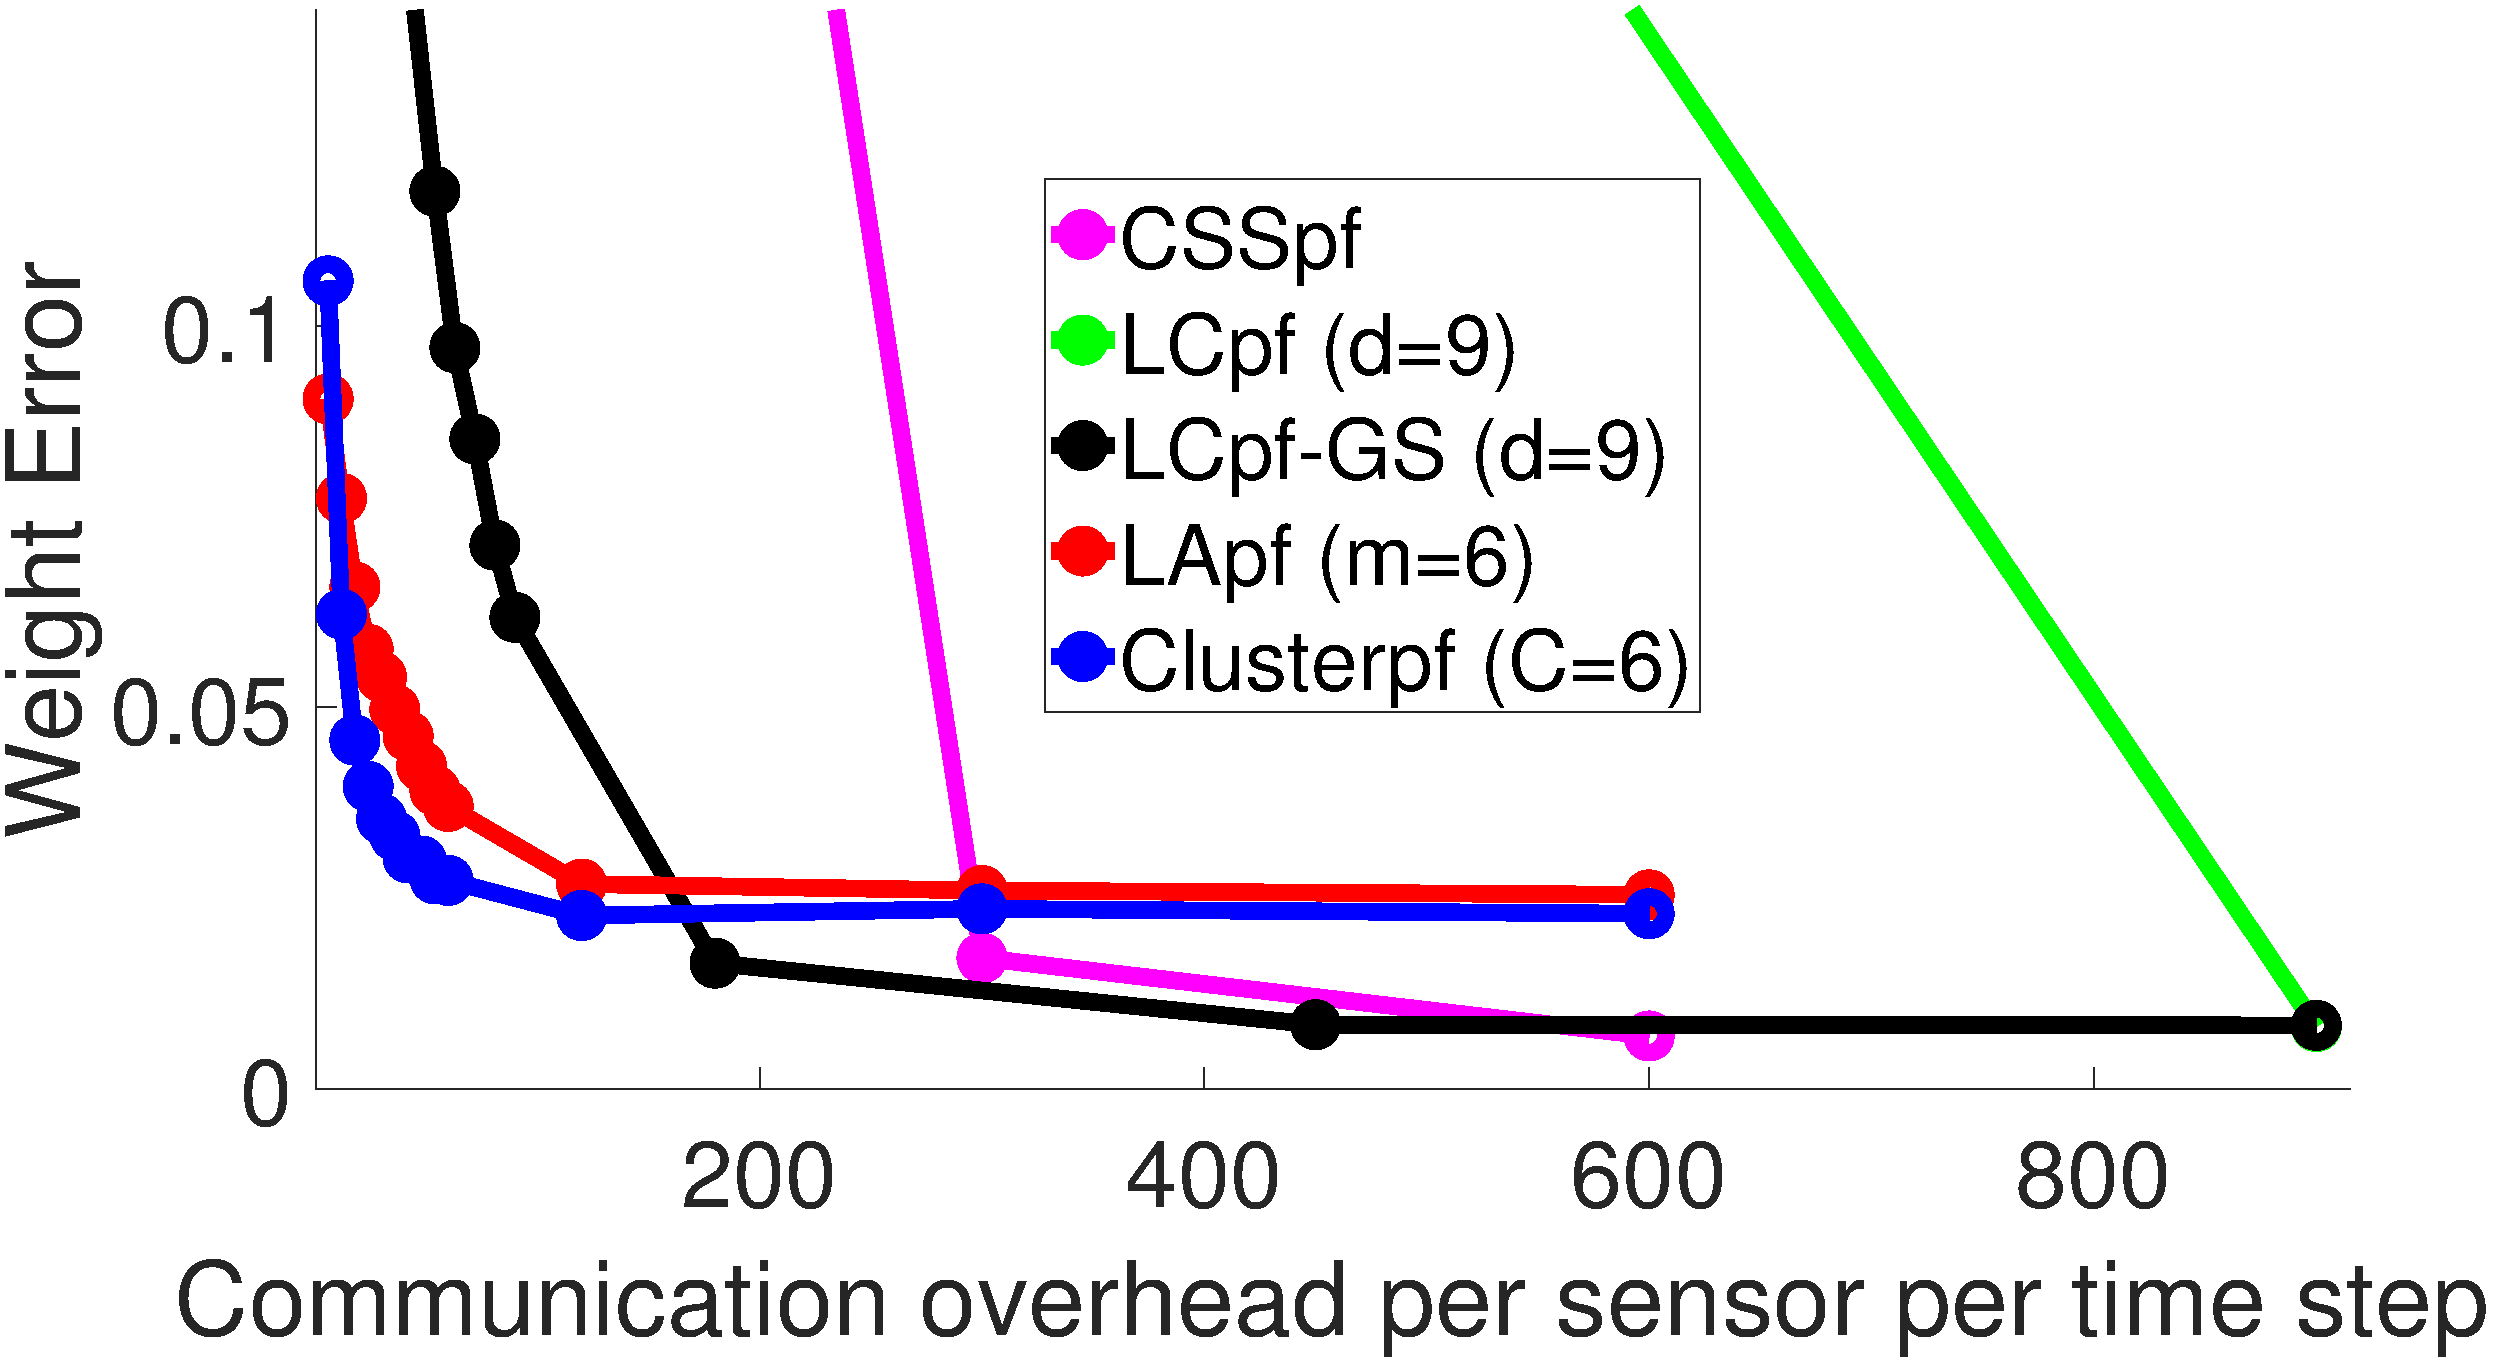
\includegraphics[width=0.49\textwidth]{Figures/Track2_bearing_WError}}
\end{subfigure}
\caption{Average RMSE and particle weights error with respect to total communication overhead per time step for track 2 ($N=500$, 200 Monte Carlo trials).}
\label{fig:Track2_results}
\end{figure}

Fig.~\ref{fig:Track3_results} shows the tracking results for track 3. Again, LApf and Clusterpf achieve robust tracking performance even with very low communication overhead. LCpf achieves good performance for $NGossip\geq 50$. CSSpf has poor performance even for $NGossip\geq 100$ even though its weight error is lowest for $NGossip \geq 30$. 

\begin{figure}
\centering
\begin{subfigure}[RMSE]
{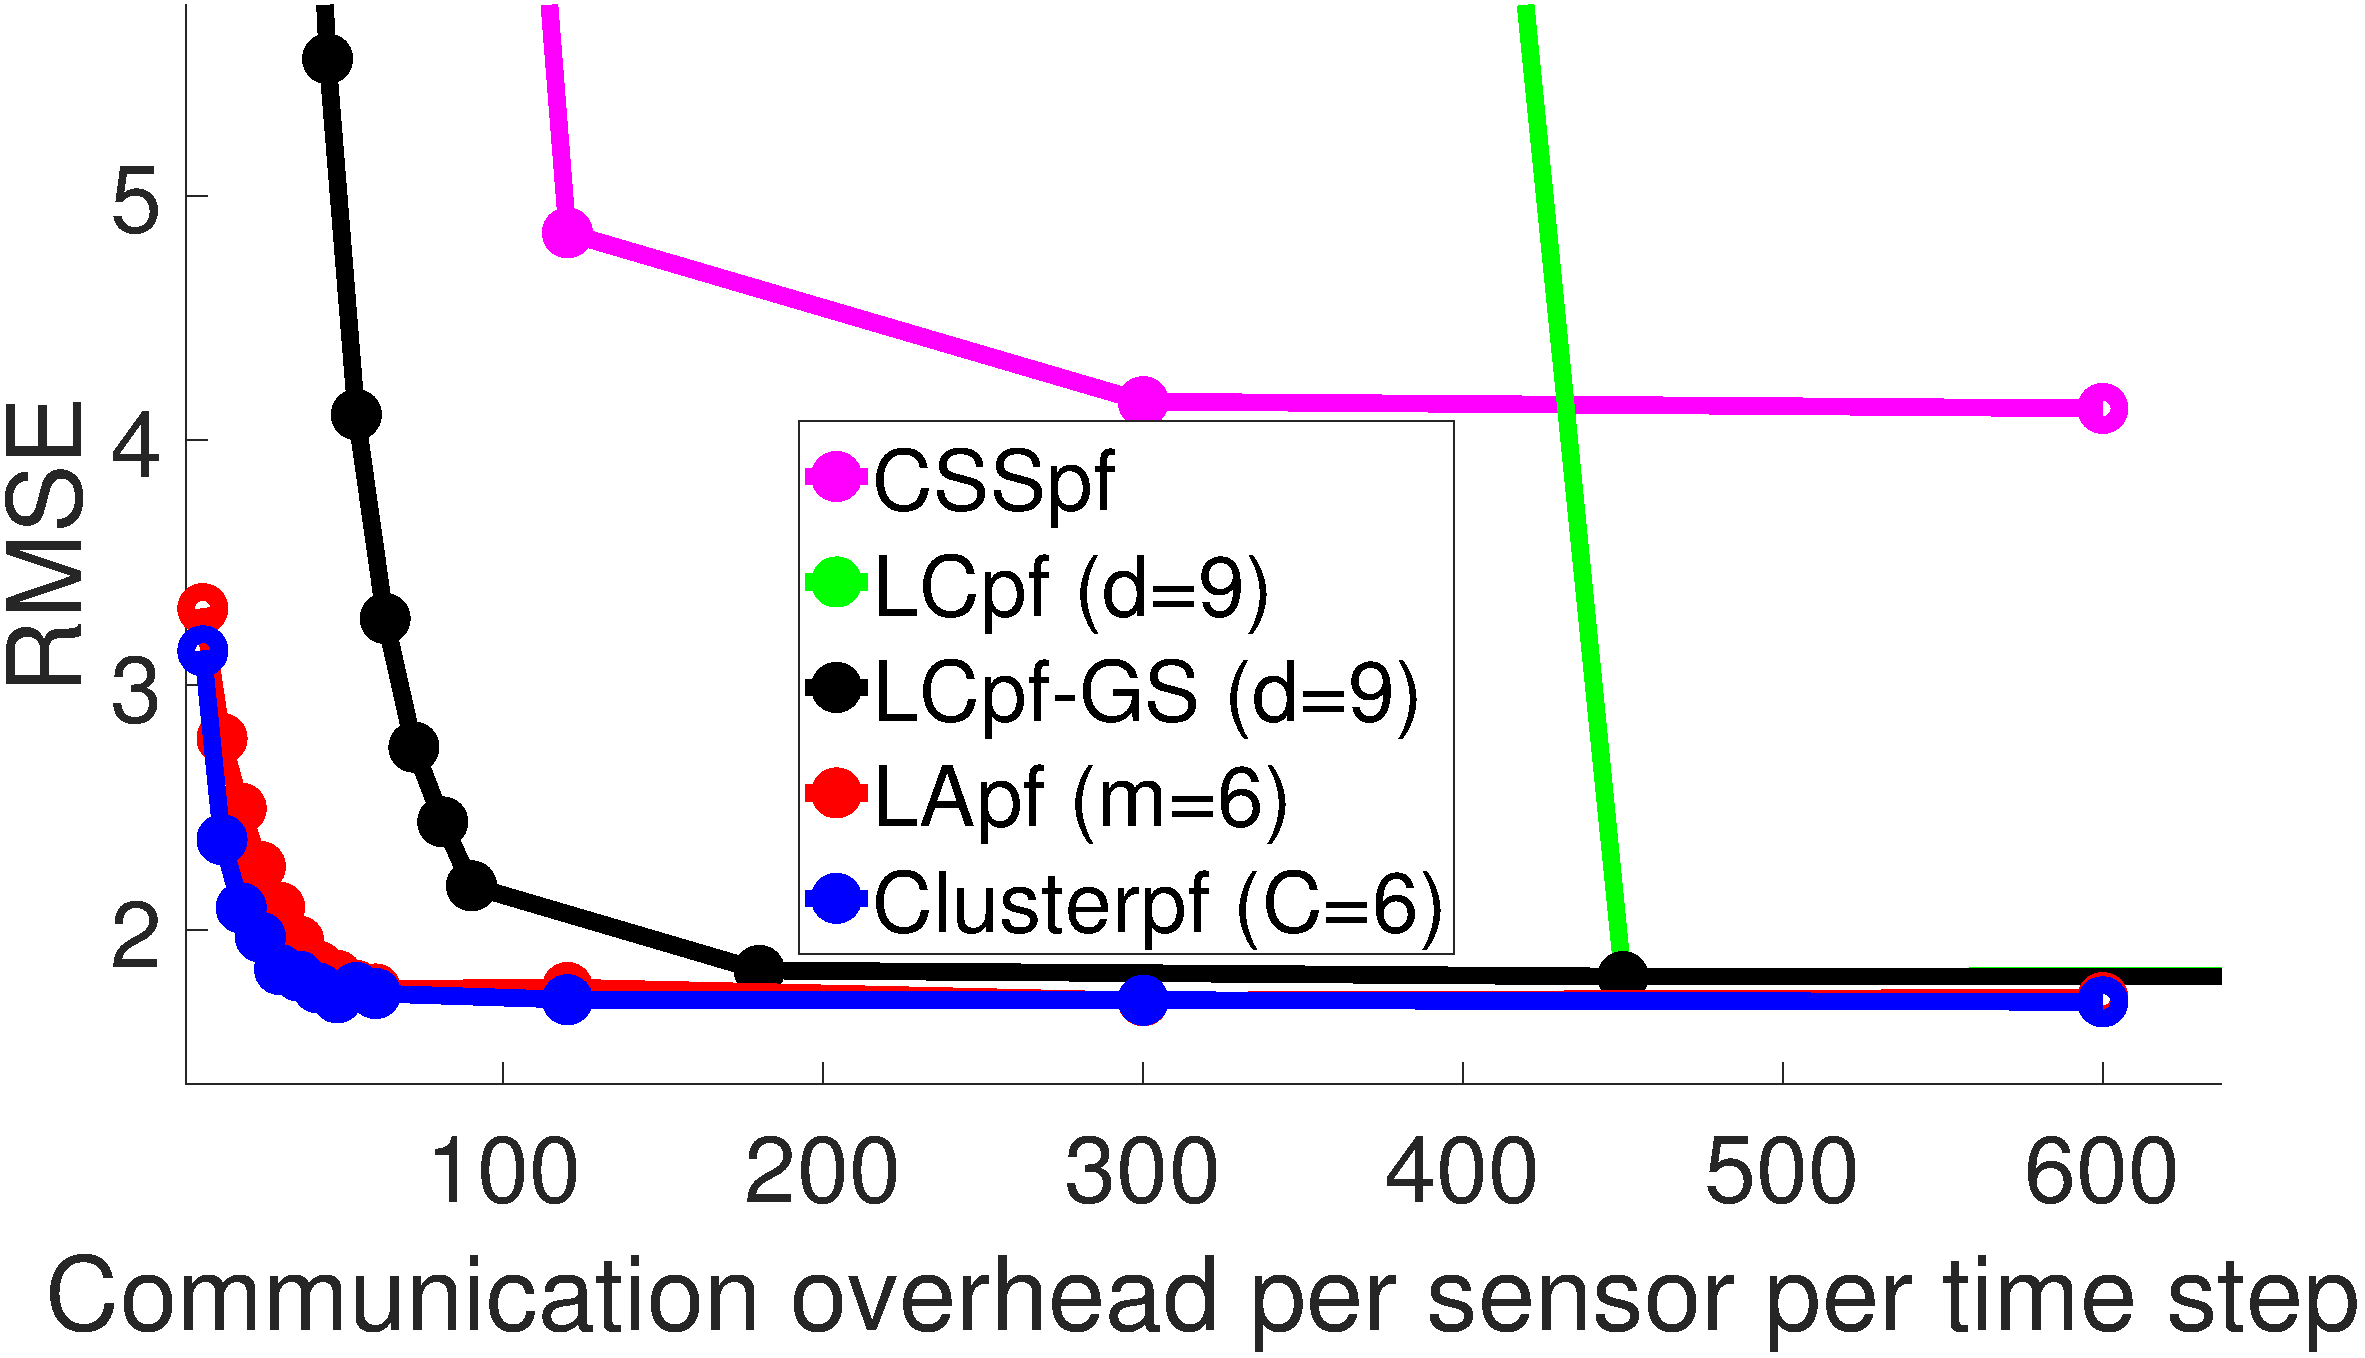
\includegraphics[width=0.49\textwidth]{Figures/Track3_bearing_RMSE}}
\end{subfigure}
\begin{subfigure}[RMSE]
{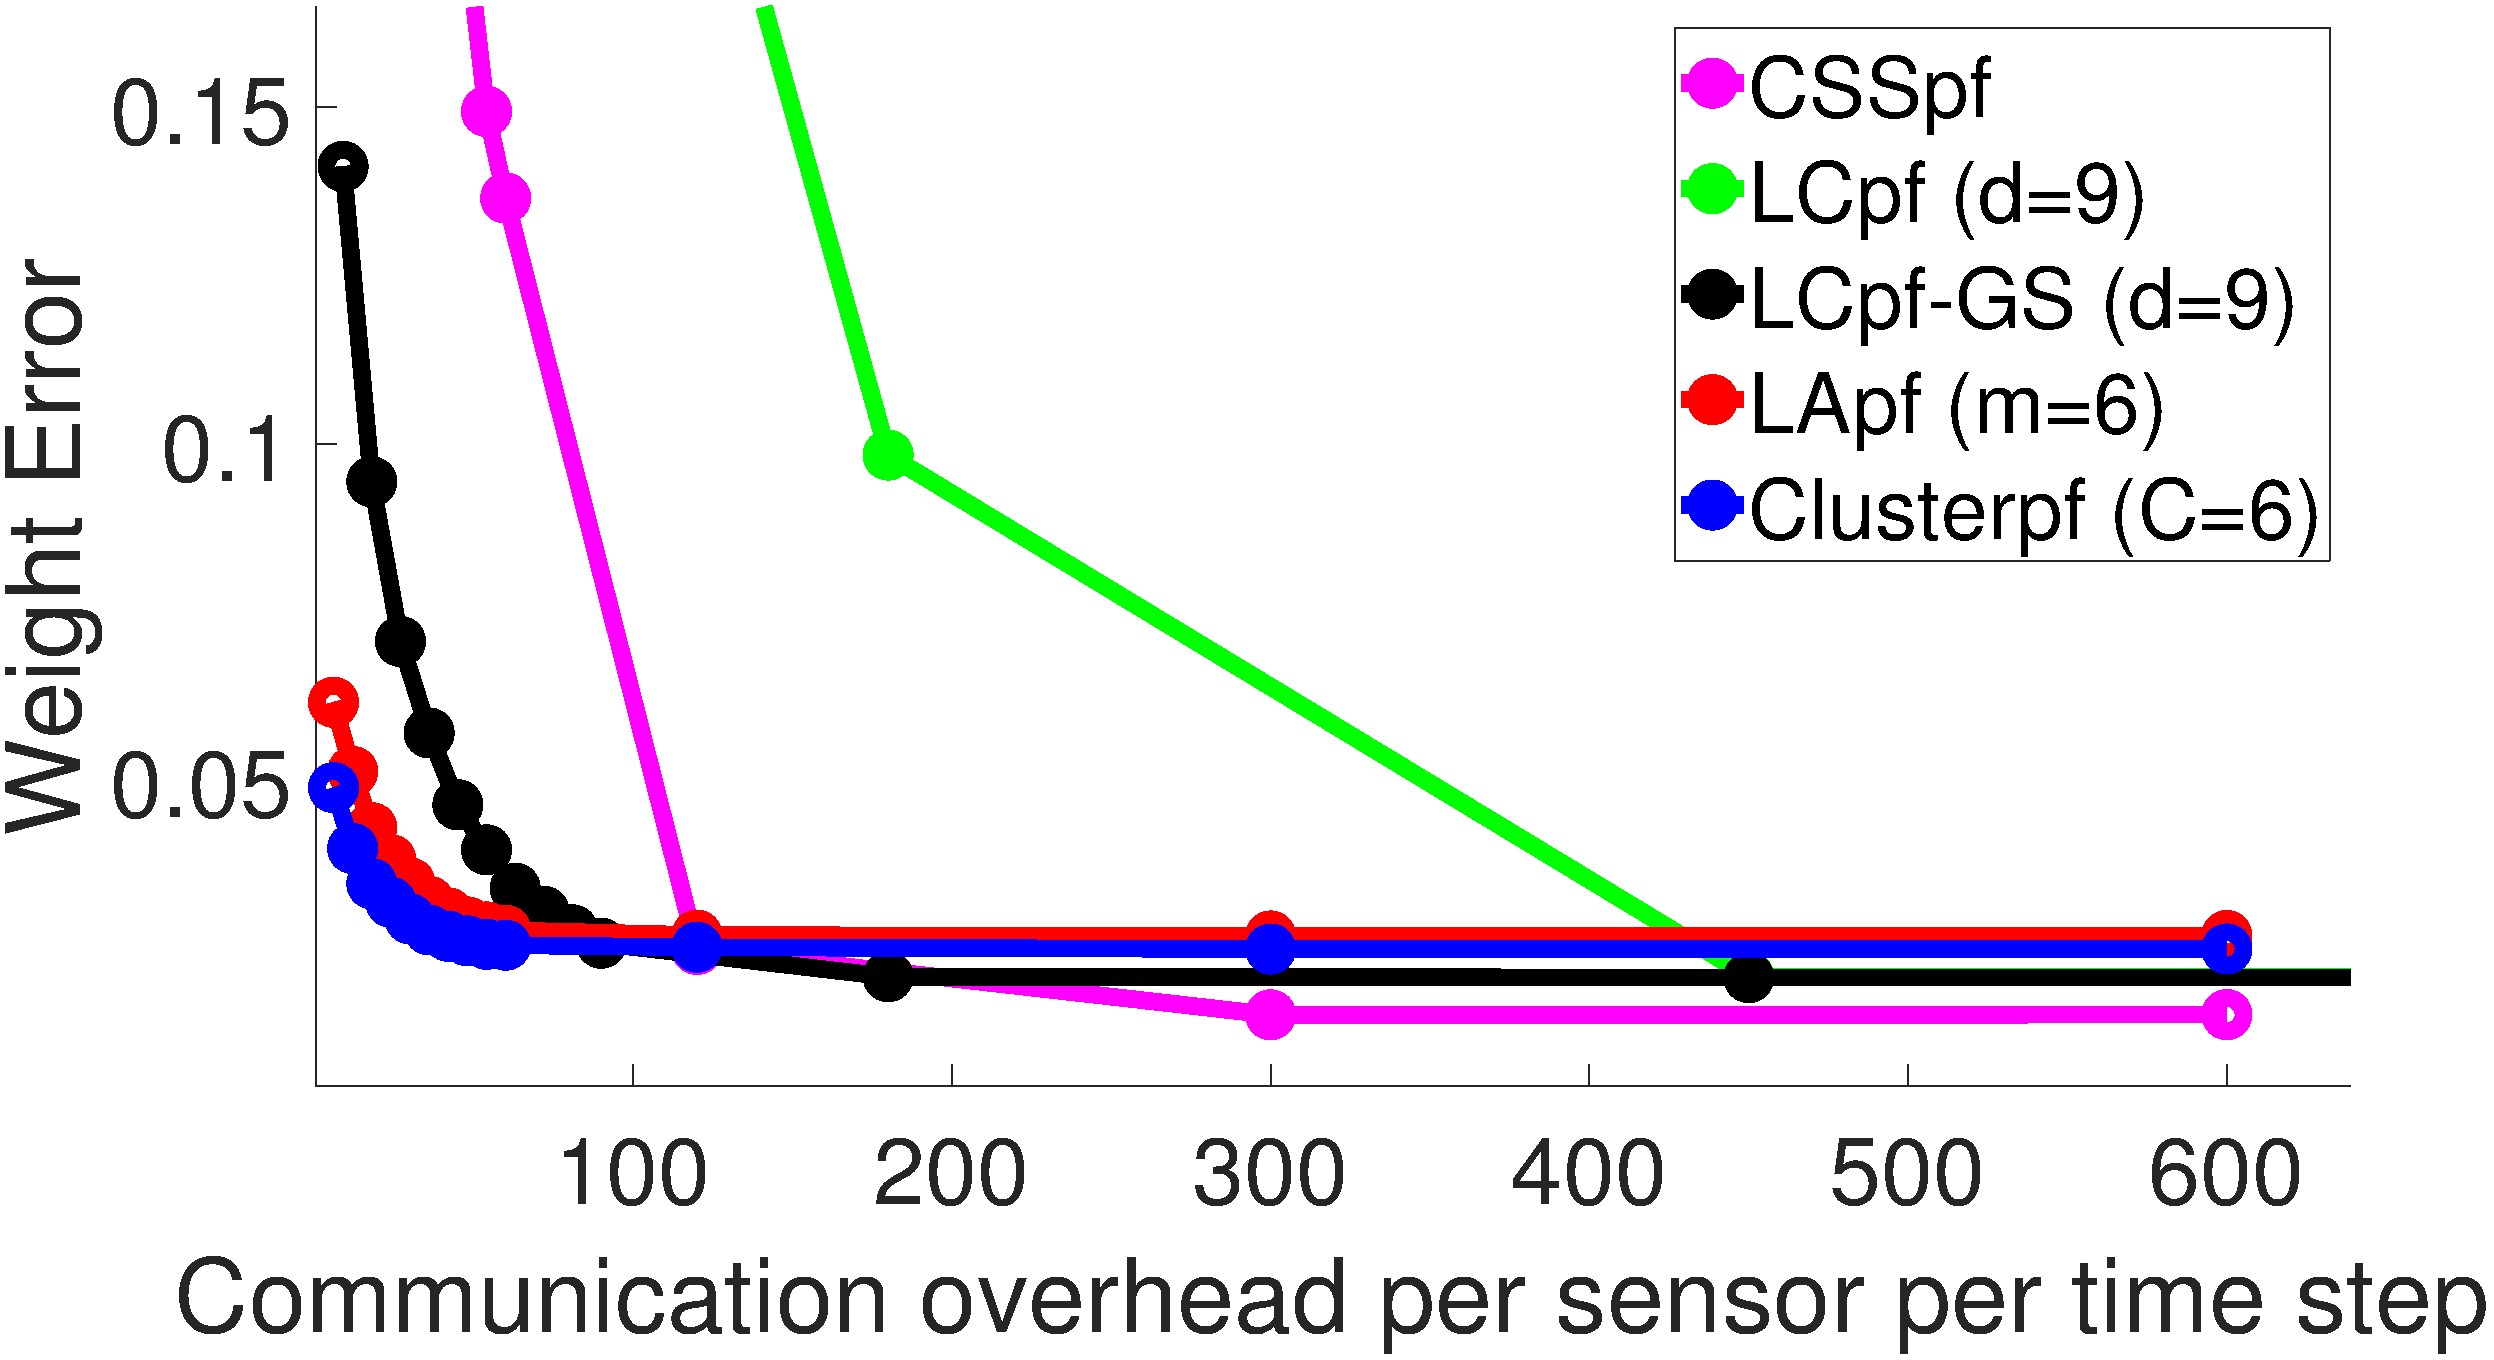
\includegraphics[width=0.49\textwidth]{Figures/Track3_bearing_WError}}
\end{subfigure}
\caption{Average RMSE and particle weights error with respect to total communication overhead per time step for track 3 ($N=500$, 200 Monte Carlo trials).}
\label{fig:Track3_results}
\end{figure}

In all three test tracks, the LApf and Clusterpf yield robust tracking performance even with very low communication overhead. The other filters may outperform LApf and Clusterpf albeit at the cost of higher overhead. In particular, the LCpf requires significantly higher communication overhead to achieve similar RMSE as the other filters. 

Fig.~\ref{fig:Track3_time} shows the average runtime of the filters. We omit the results for tracks 1 and 2 since the trends are similar. The LApf has the highest runtime due to the overhead of eigendecomposition. The Clusterpf has the second highest runtime. The other filters have similar low runtime. We note that increasing $NGossip$ does not increase total runtime due to our implementation of the gossip algorithms. 

\begin{figure}
\centering
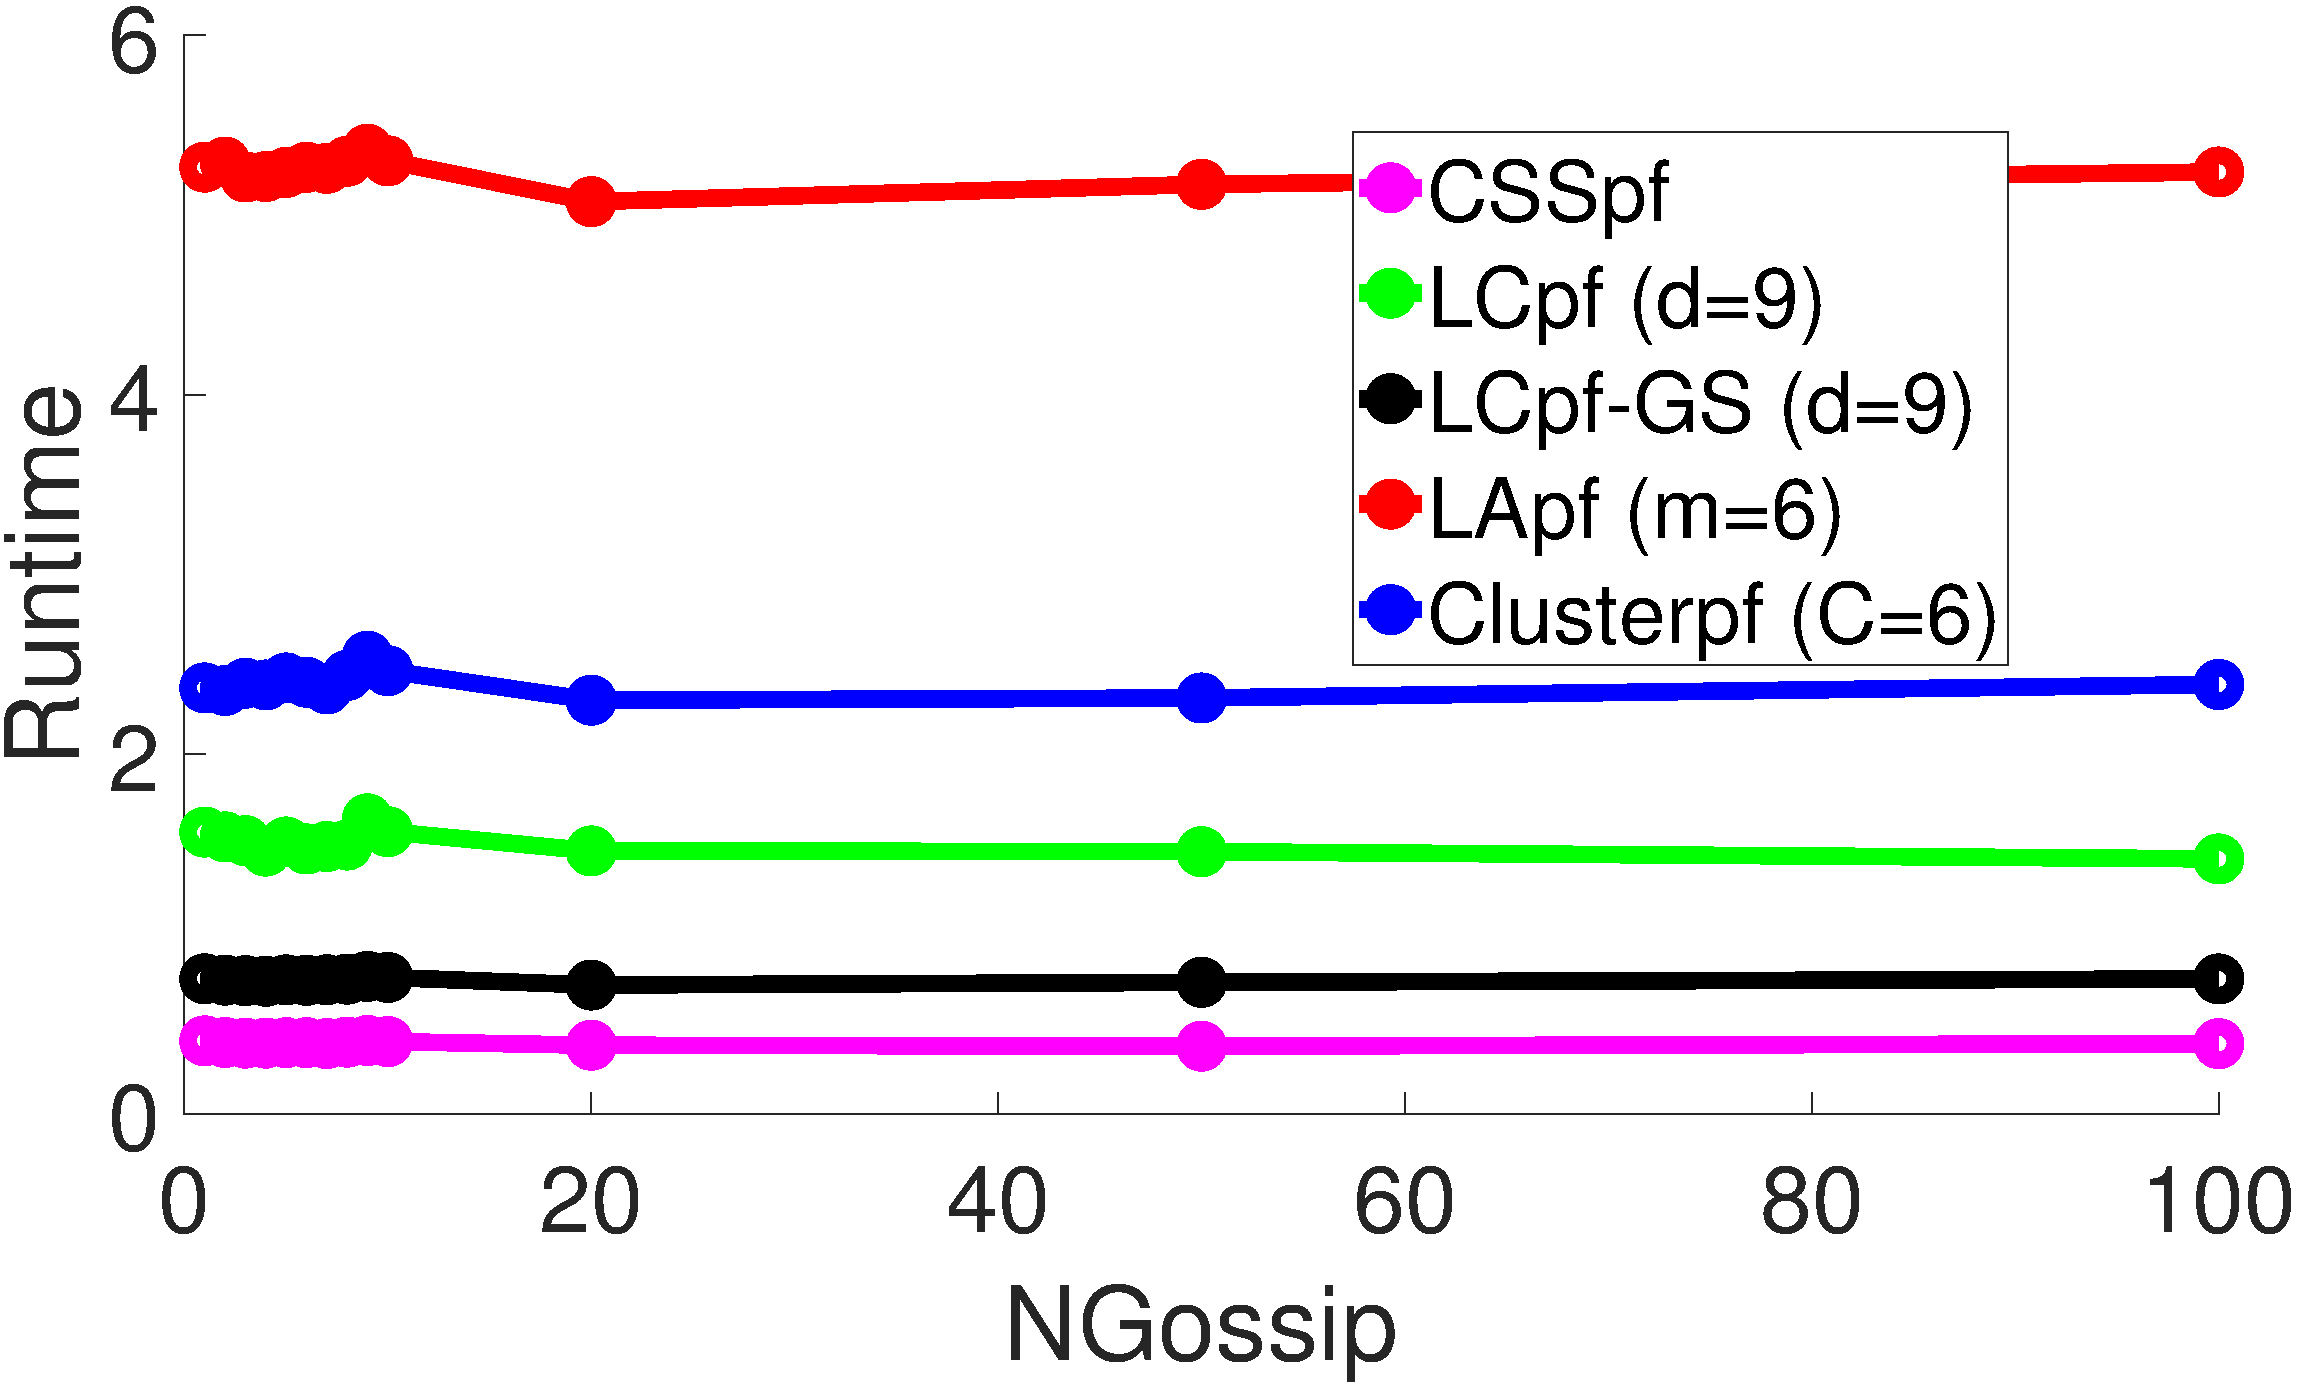
\includegraphics[width=0.5\textwidth]{Figures/Track3_bearing_time}
\caption{Average total runtime for track 3}
\label{fig:Track3_time}
\end{figure}

\subsection{Sensitivity analysis of particle filters}
Simulation results in the previous sections suggest that LApf and LCpf are considerably less susceptible to gossiping noise than the other three filters. In this section, we conduct a sensitivity analysis of all filters.

We run a centralized BSpf for all three tracks. At each time step, we re-compute the posterior particle weights using all distributed filters. We then compute and report the discrepancy of approximate and exact particle weights (i.e., $||W_{BS}-W_{CSS}||_2$).

The goal is to understand each filter's susceptibility to gossiping error. The aggregate values are first calculated exactly without gossiping; then we inject perturbation into the aggregate values. Let $\alpha$ denote the true aggregate value and $x$ the perturbation level, then the final aggregate value used in weight computation is $\alpha(1+ x/100)$ or $\alpha(1- x/100)$ with equal probability. Note that, in this definition, perturbation level is equal to the AER. We choose this approach so we can control the AER exactly without fine-tuning the number of gossip iterations. 

We repeat this test but run a fixed number of gossip iterations for all filters. The perturbations in this case are generated from gossiping errors. 

Fig.~\ref{fig:perturbation_results} shows the average weight discrepancy with respect to perturbation level and number of gossip iterations. In all three tracks, LCpf has the worst performance by far followed by CSSpf. Even at very low perturbation level, the weight discrepancy of LCpf can go above 0.2. On the other hand, LCpf-GS and LApf have consistently the best performance with LApf having an edge for perturbation $>100$. And we note that, for all values of $NGossip$, the weight discrepancy of LApf and Clusterpf never exceeds 0.2. 

\begin{figure}
\centering
\begin{subfigure}[Track 1]
{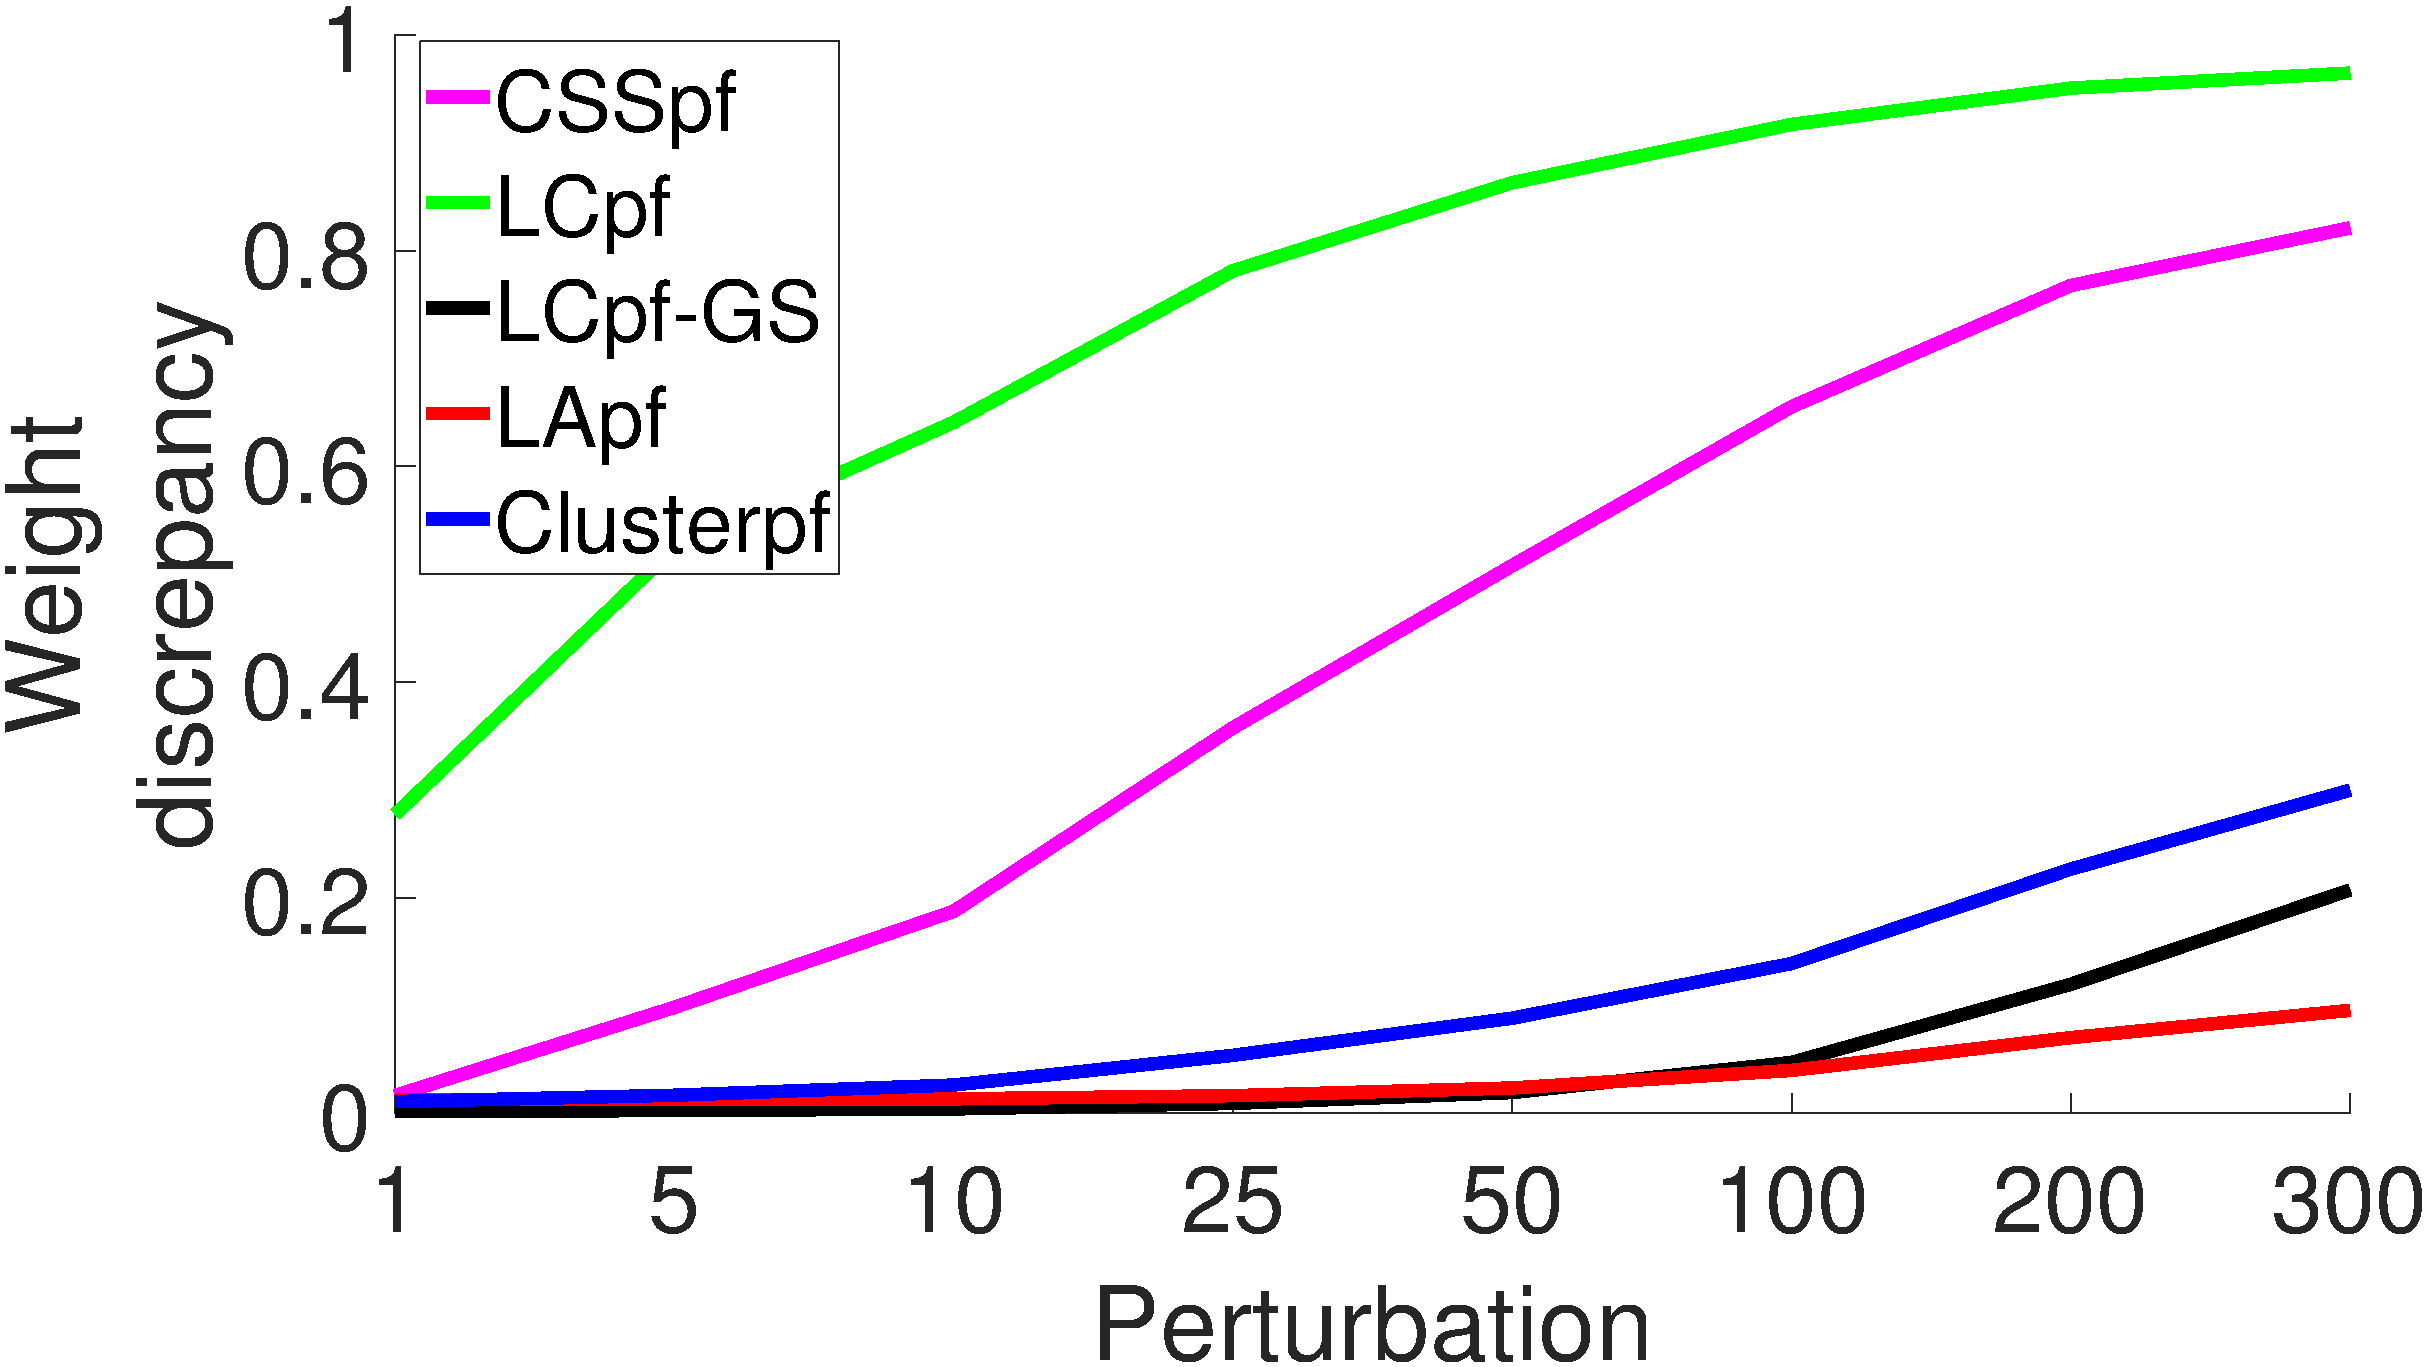
\includegraphics[width=0.49\textwidth]{Figures/curve_perturbation_track1}}
\end{subfigure}
\begin{subfigure}[Track 1]
{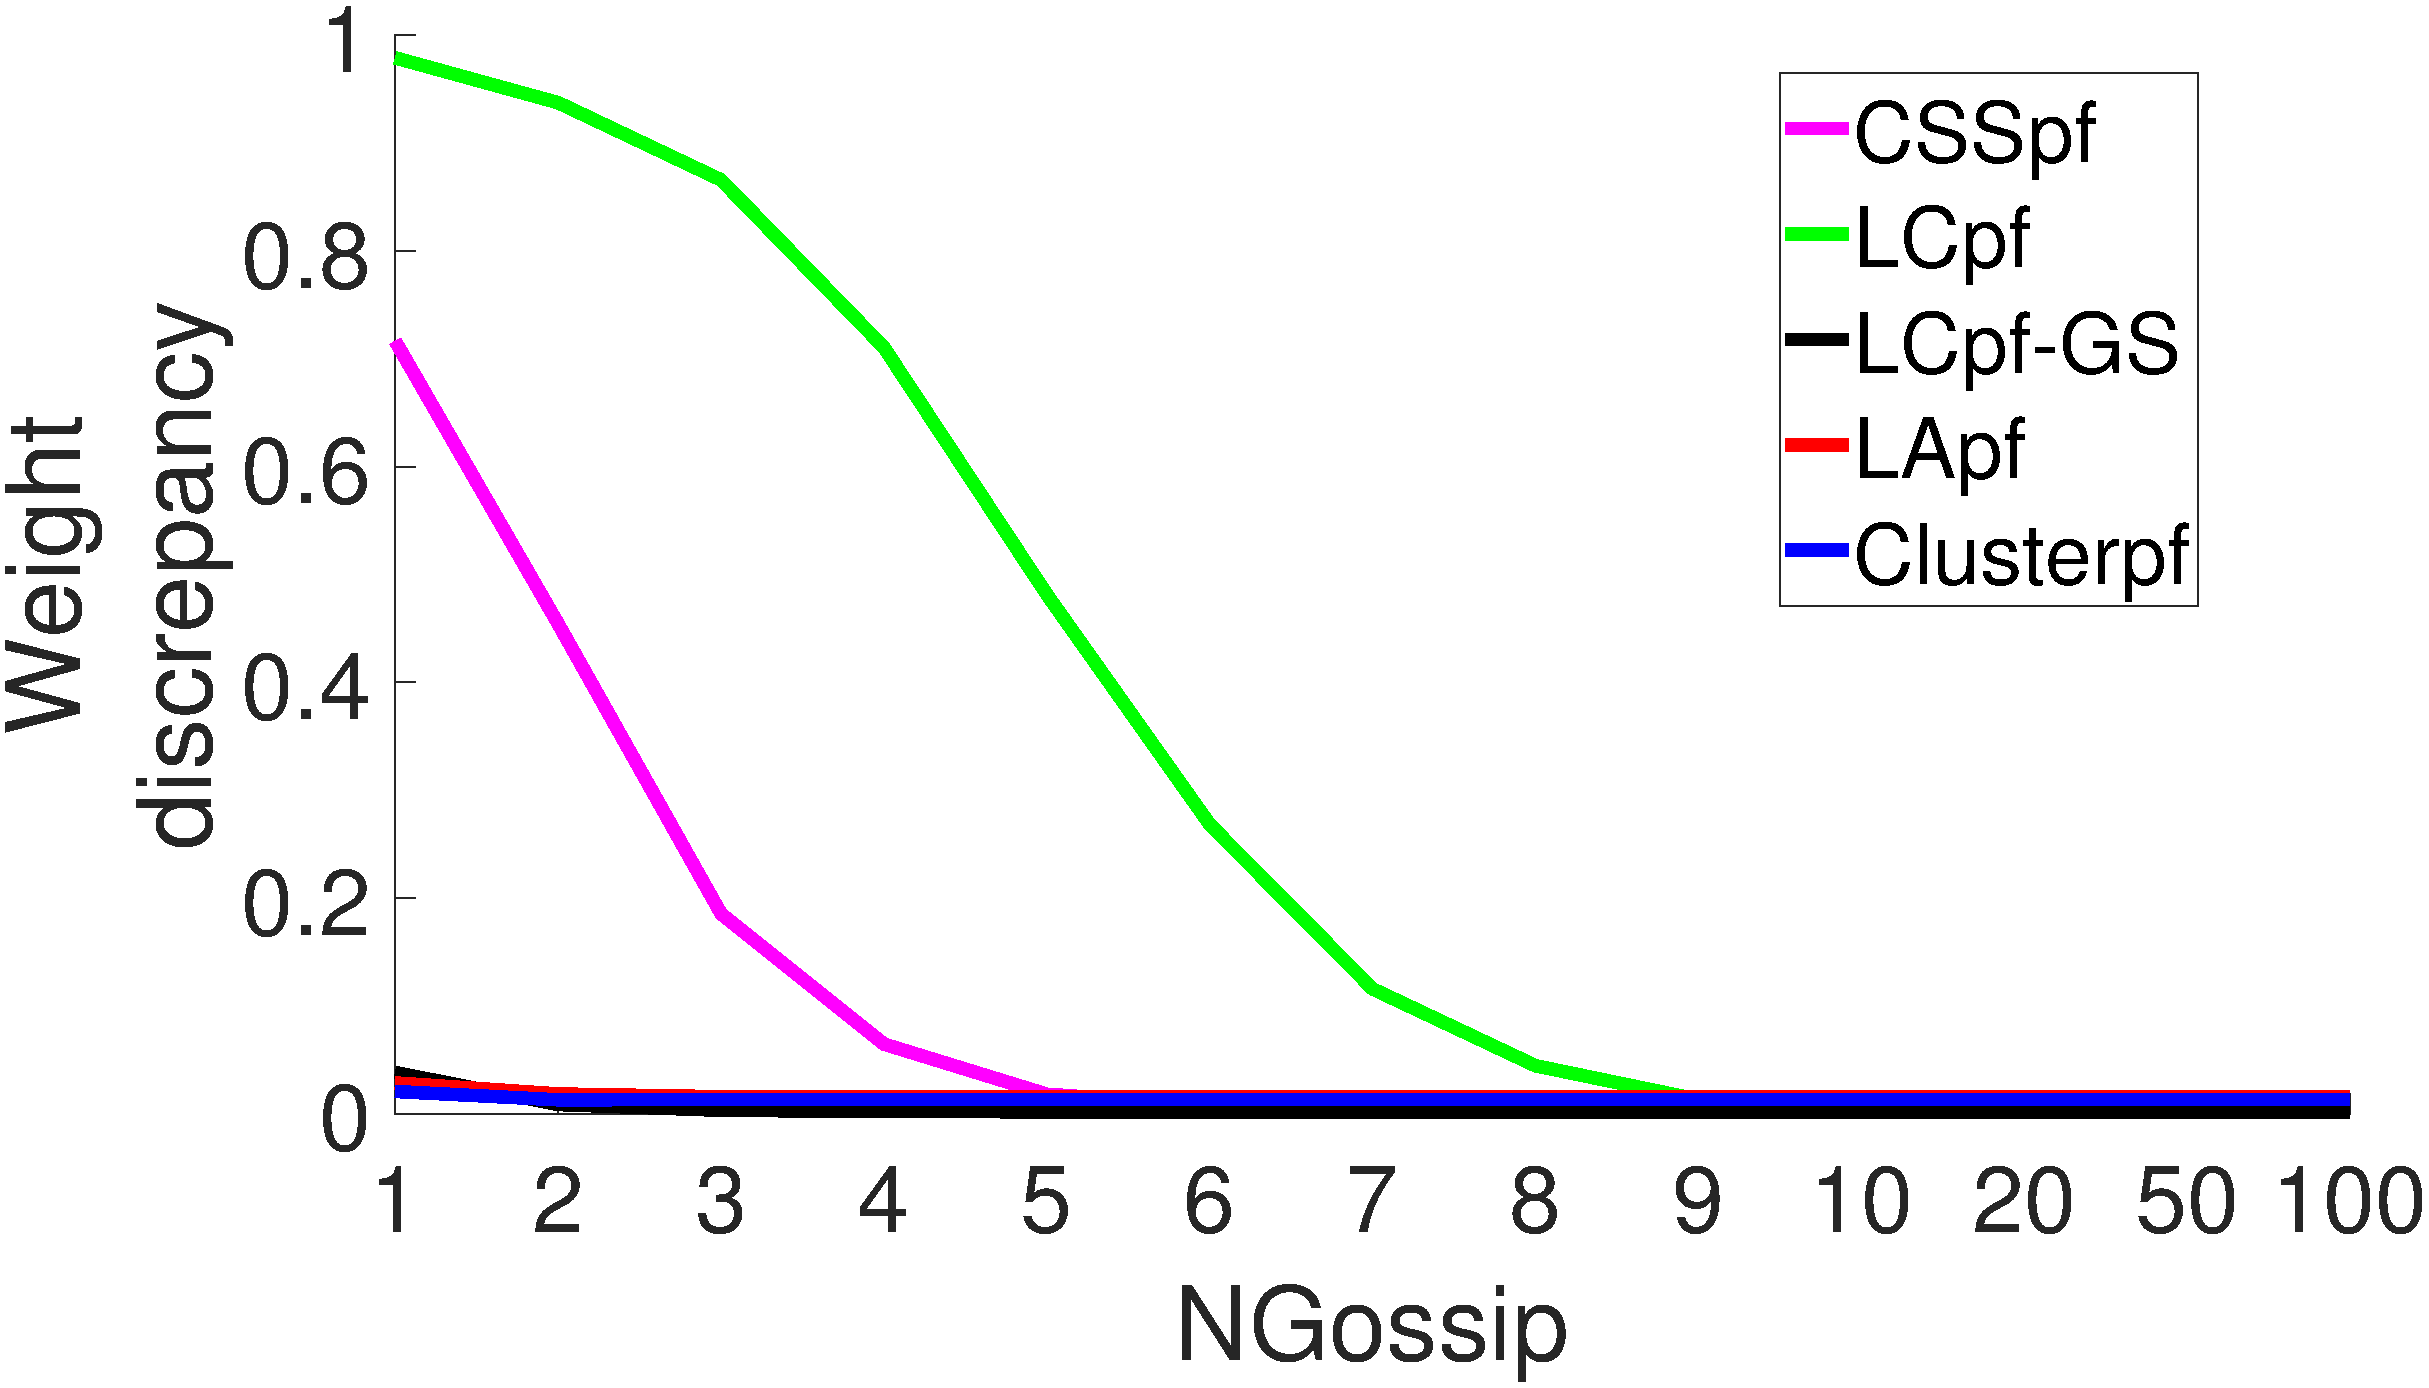
\includegraphics[width=0.49\textwidth]{Figures/curve_perturbationGossip_track1}}
\end{subfigure}
\begin{subfigure}[Track 2]
{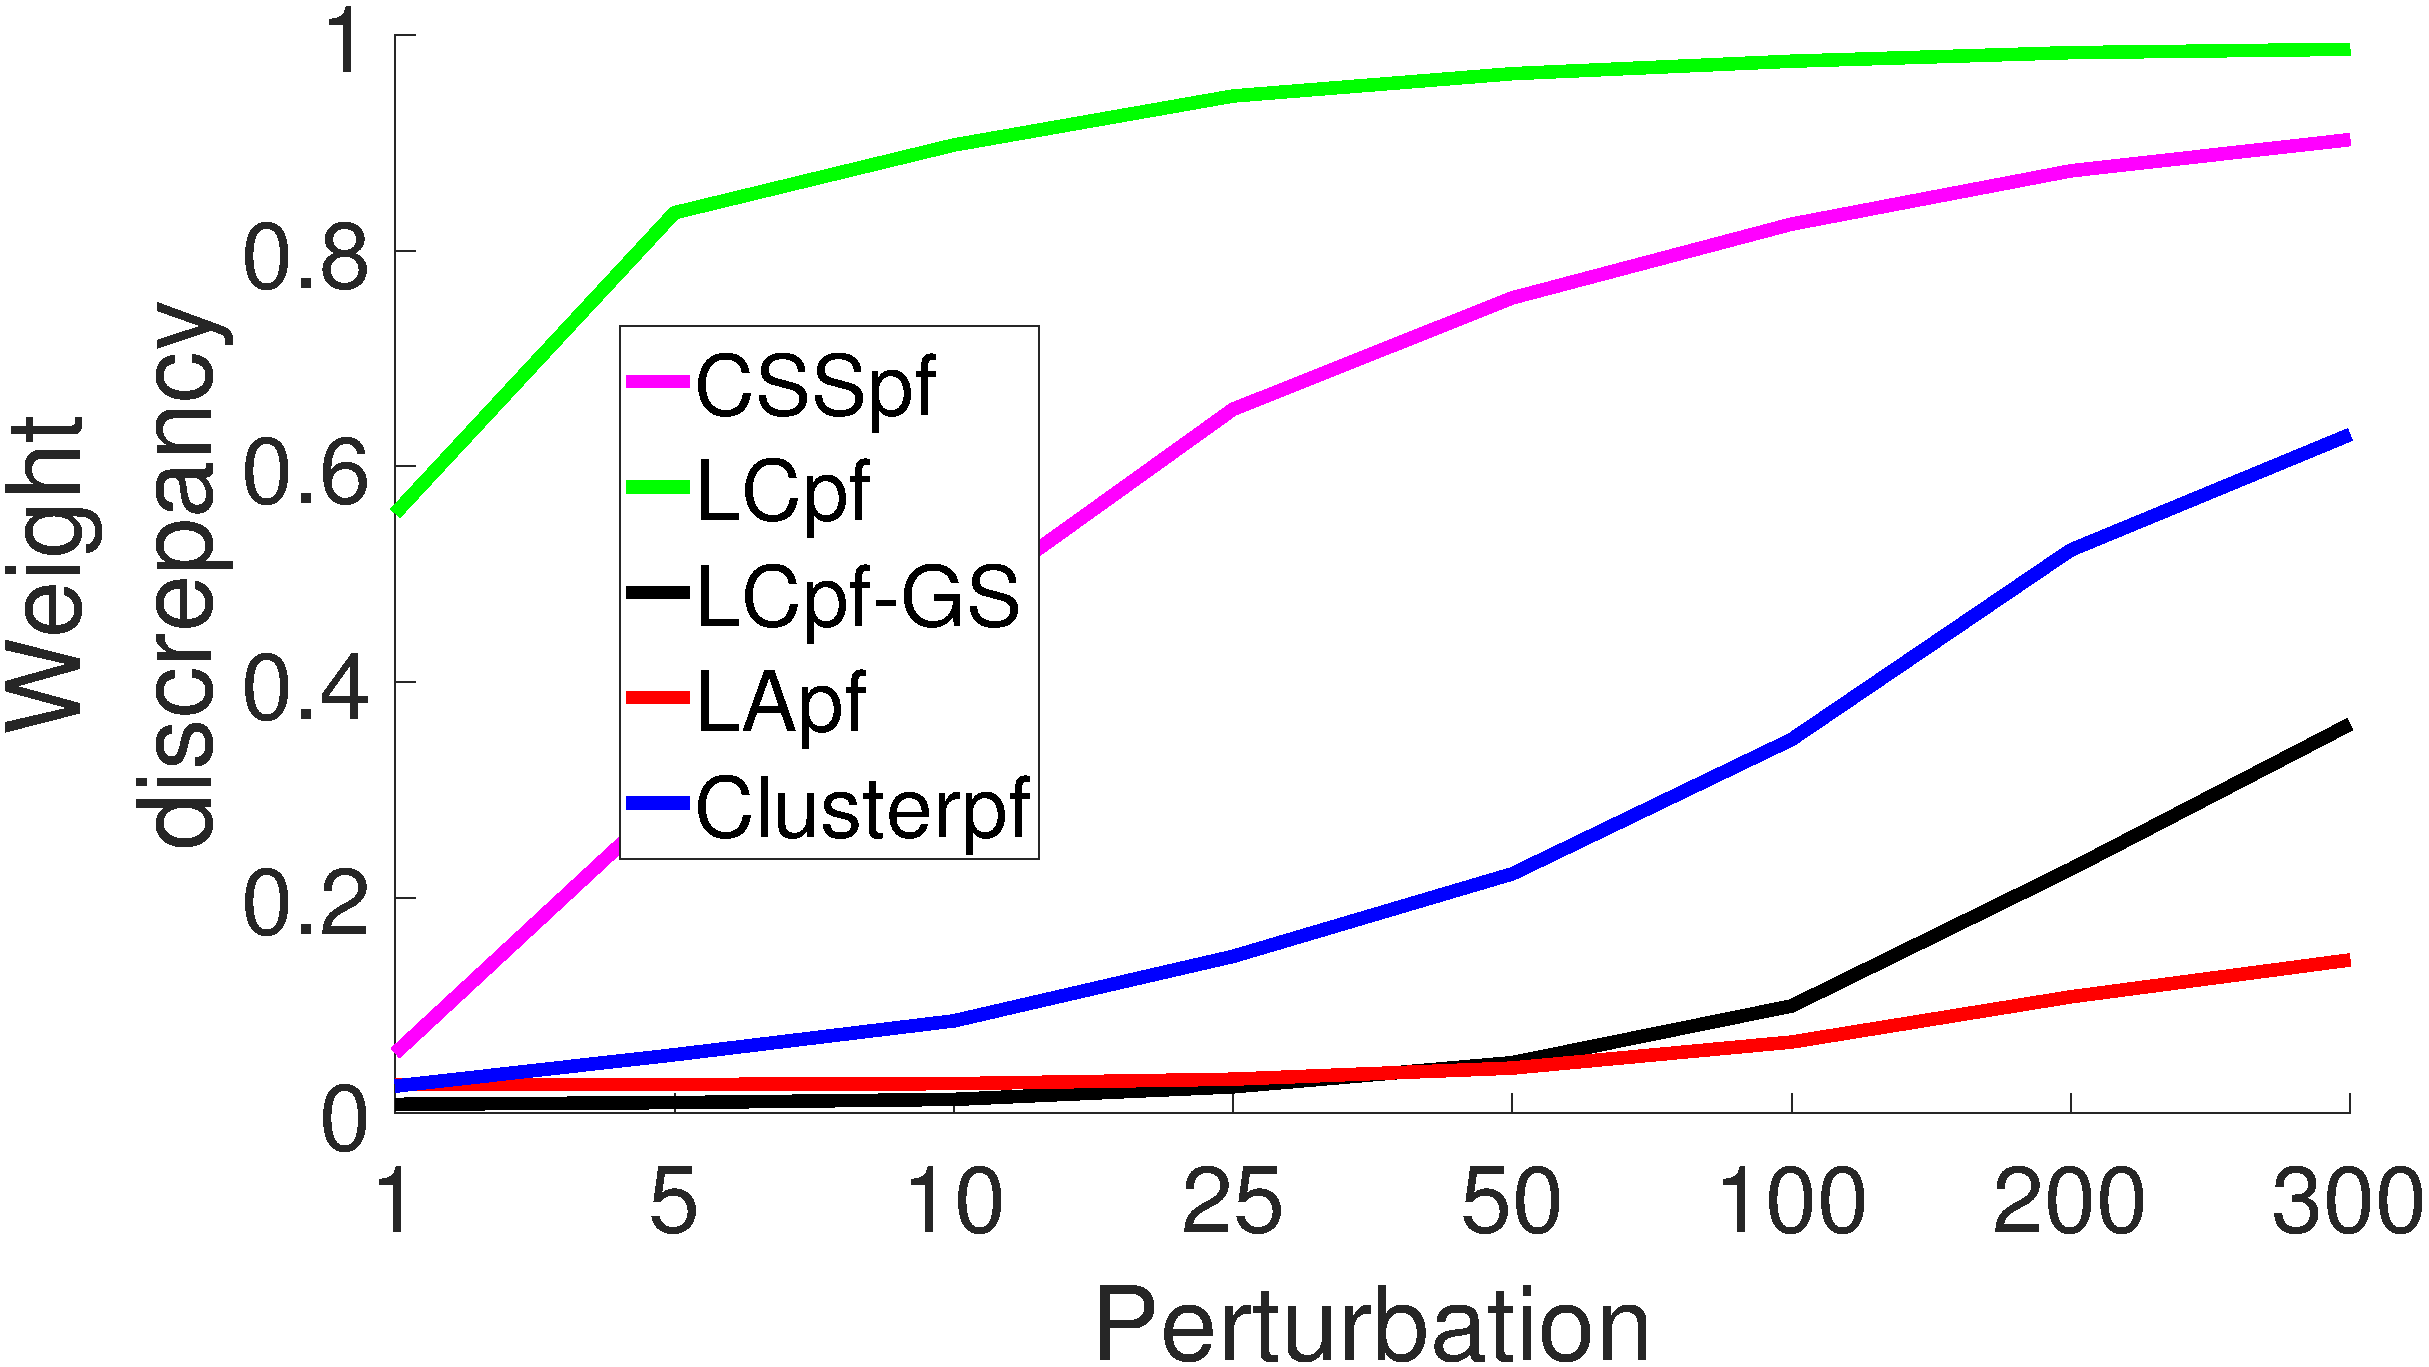
\includegraphics[width=0.49\textwidth]{Figures/curve_perturbation_track2}}
\end{subfigure}
\begin{subfigure}[Track 2]
{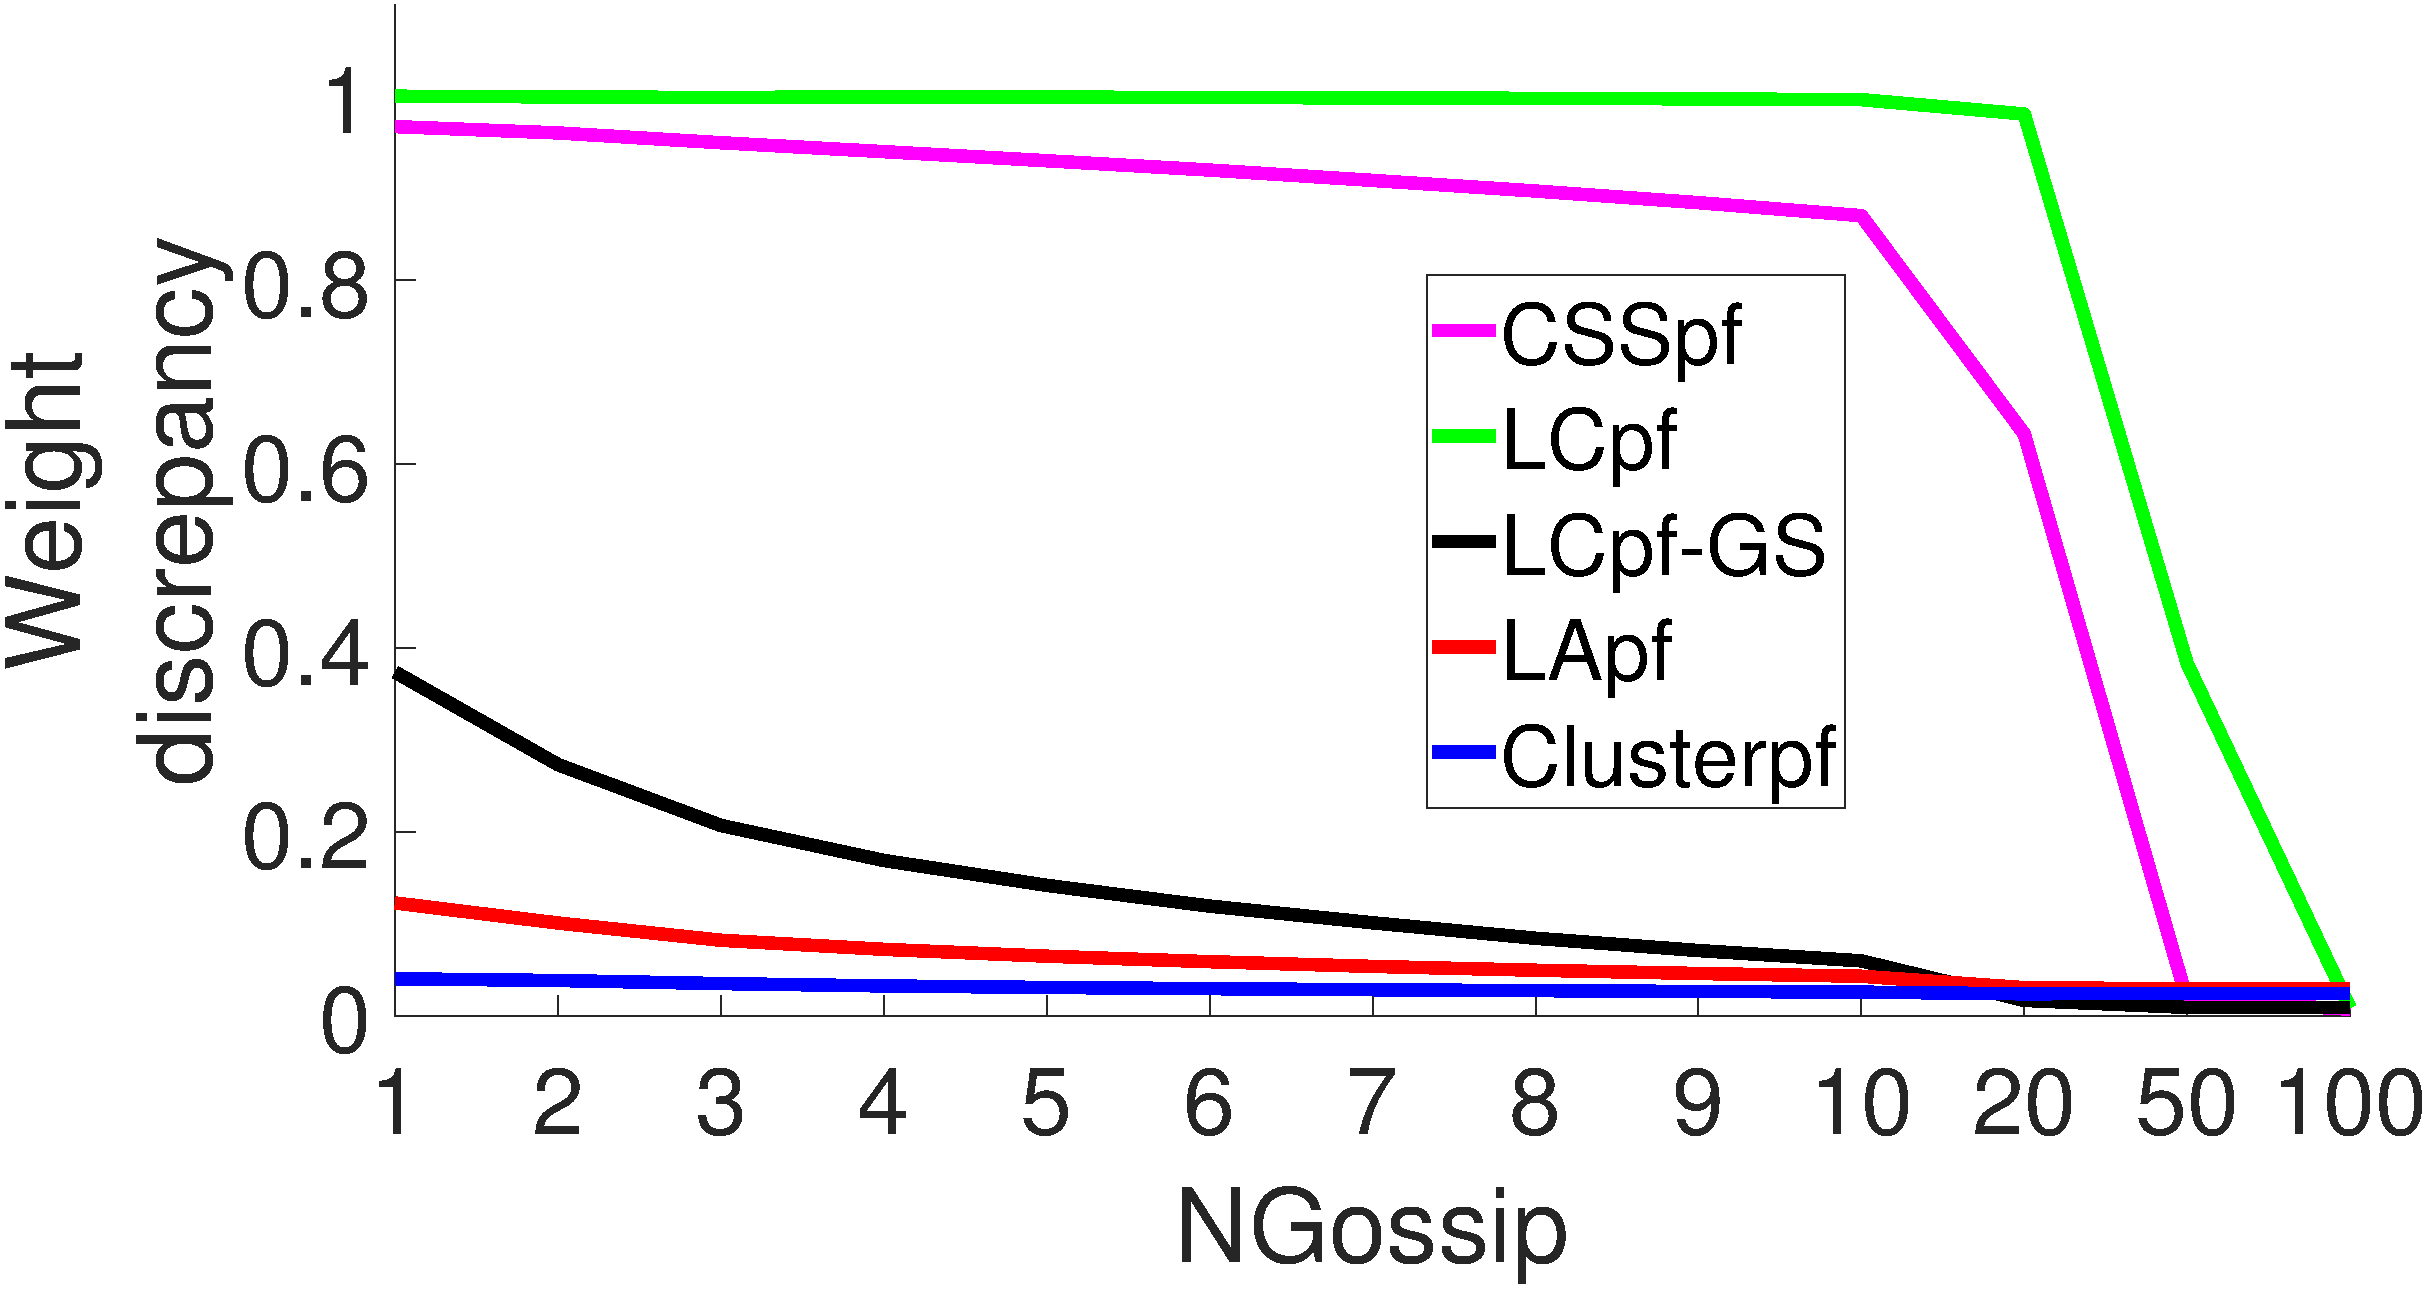
\includegraphics[width=0.49\textwidth]{Figures/curve_perturbationGossip_track2}}
\end{subfigure}
\begin{subfigure}[Track 3]
{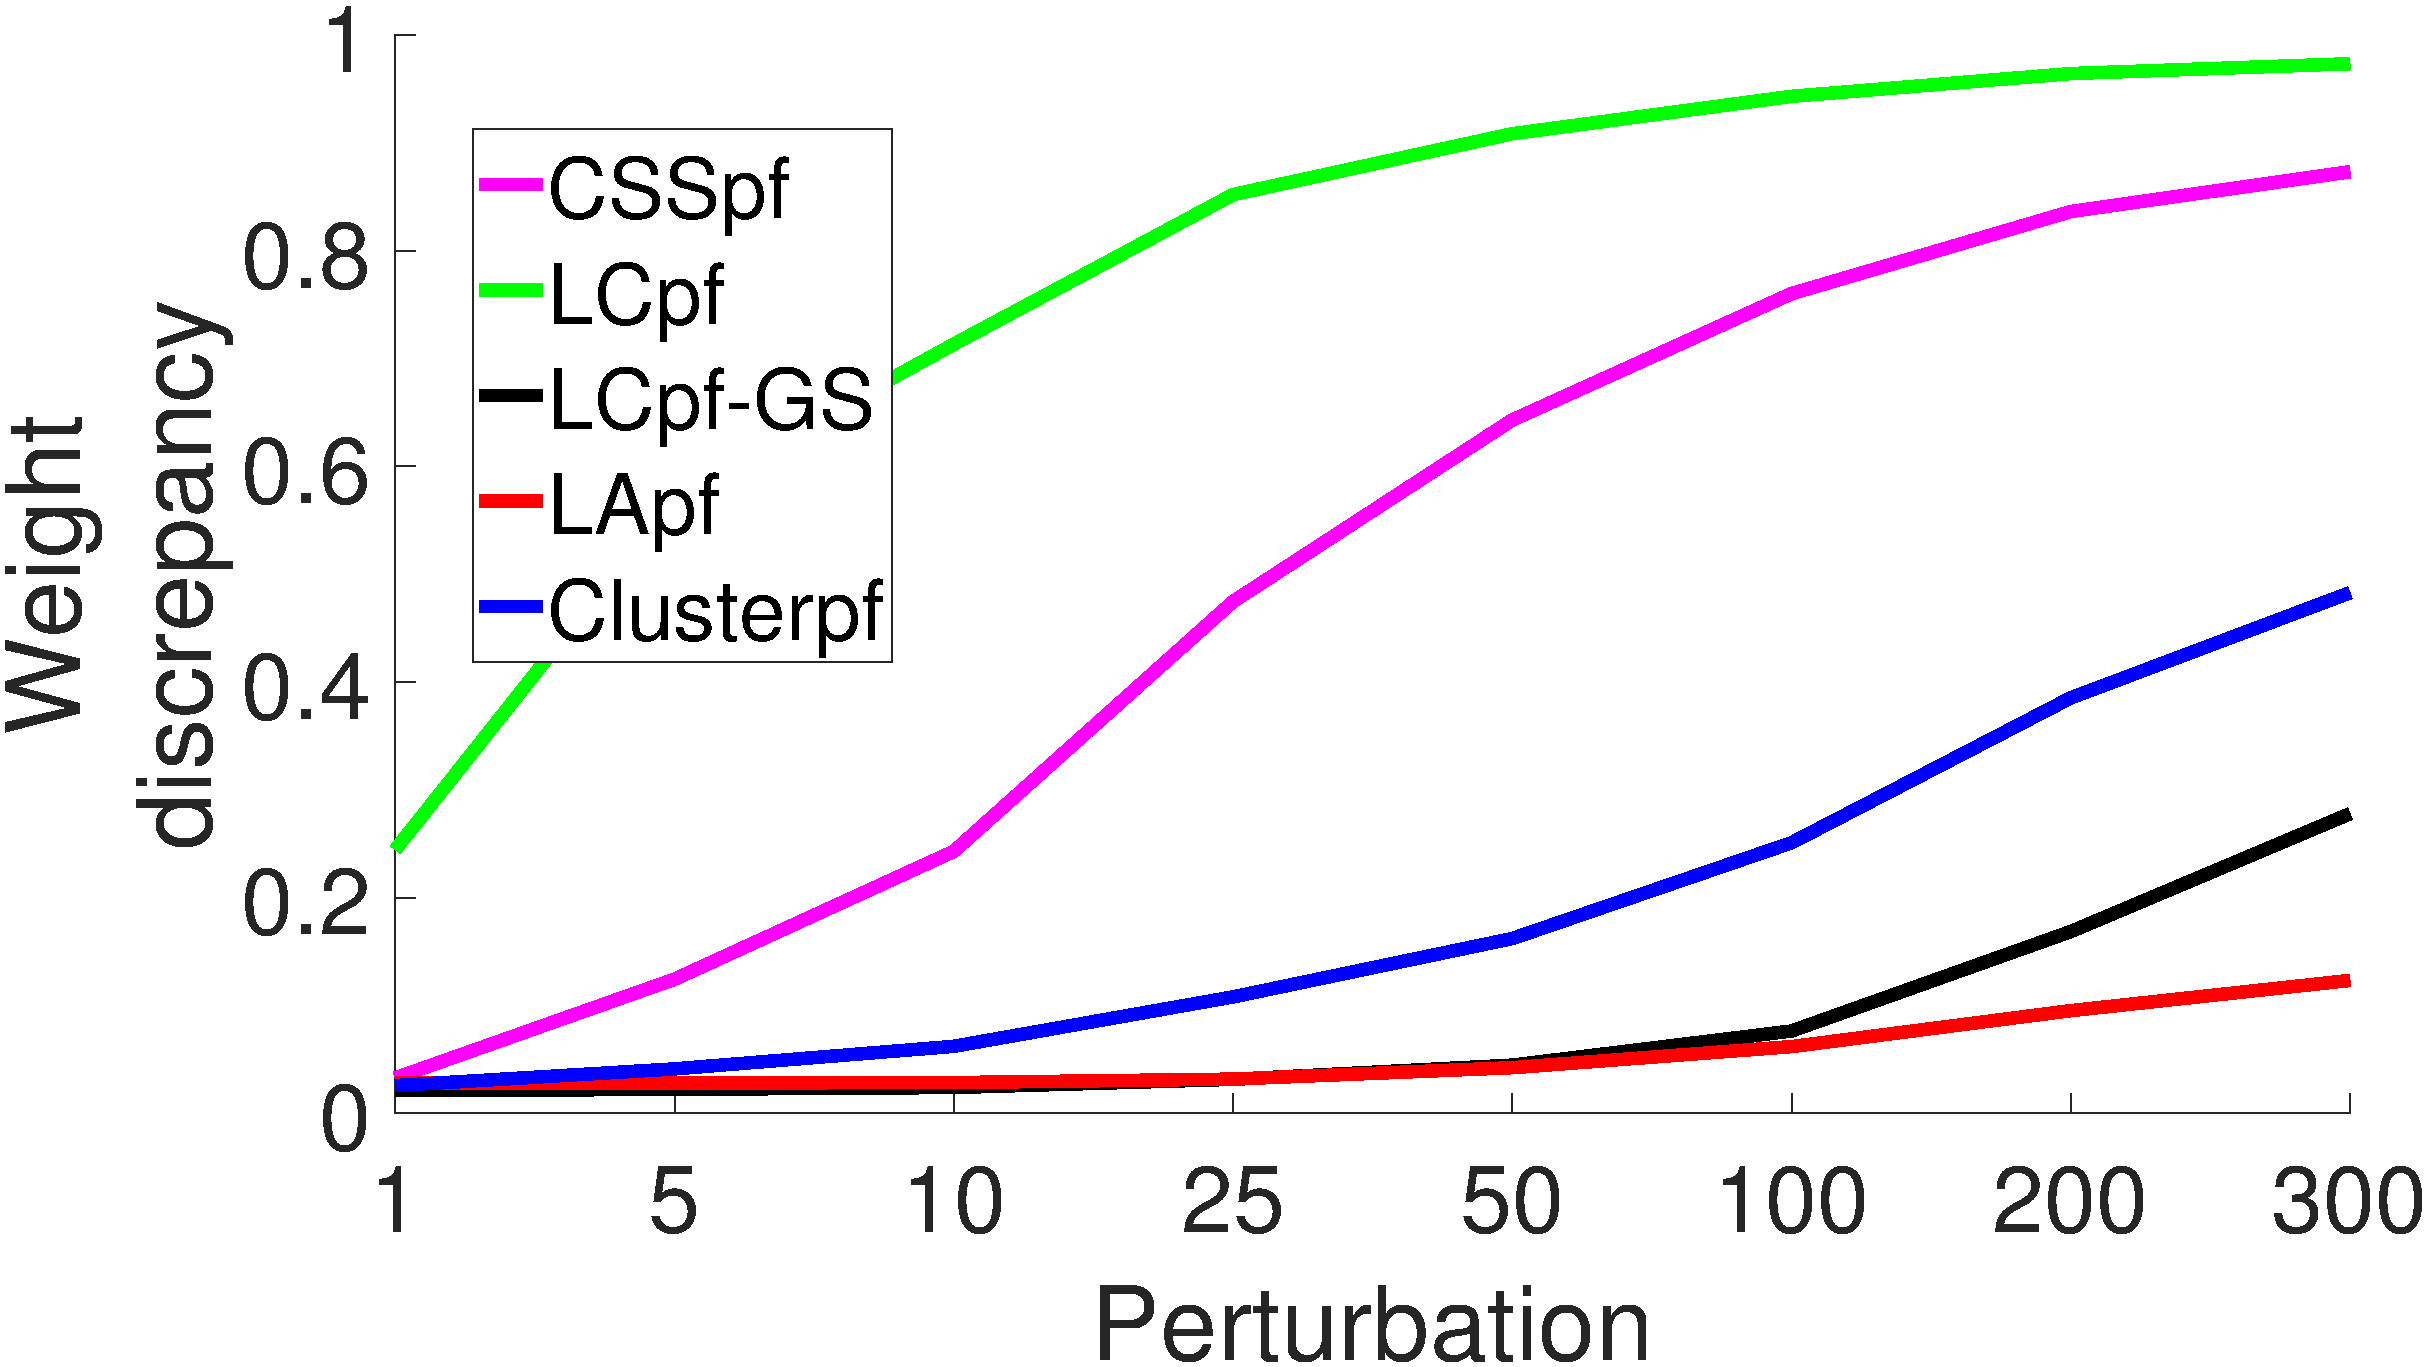
\includegraphics[width=0.49\textwidth]{Figures/curve_perturbation_track3}}
\end{subfigure}
\begin{subfigure}[Track 3]
{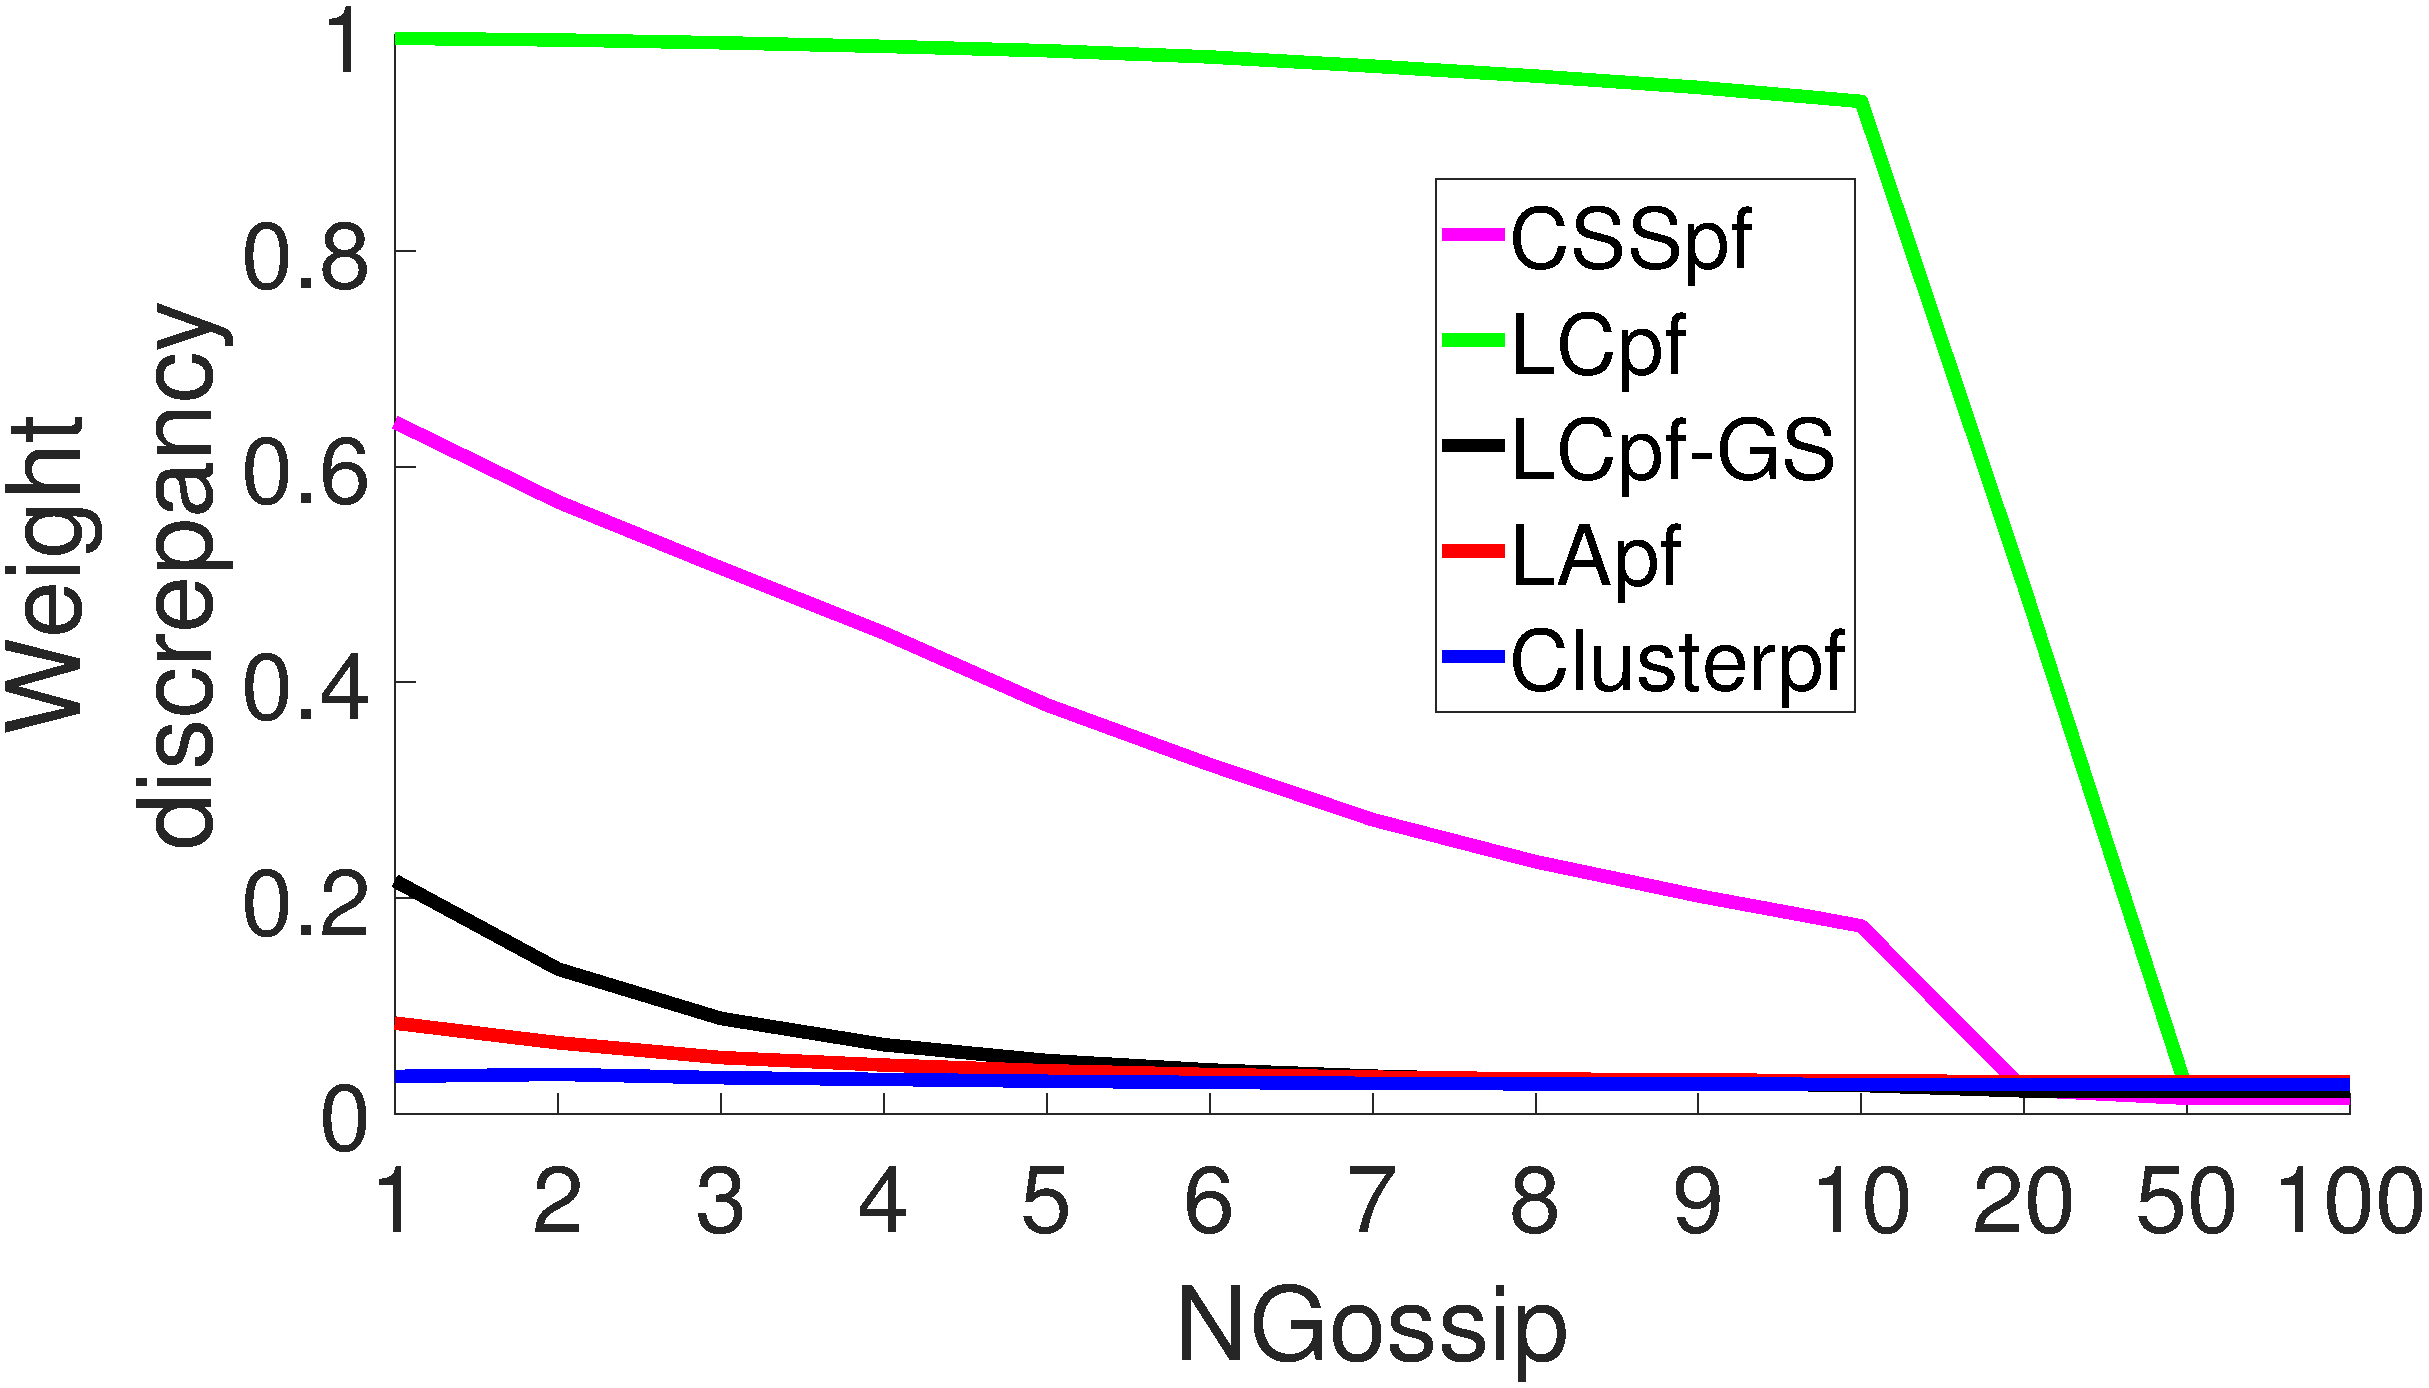
\includegraphics[width=0.49\textwidth]{Figures/curve_perturbationGossip_track3}}
\end{subfigure}
\caption{Average weight discrepancy between the exact particle weights (BSpf) and approximate particle weights (LCpf, LApf, Clusterpf) with respect to perturbation and NGossip. A perturbation of $x$ represents $x\%$ shift from the true aggregate value. $N=500$, $d=1,m=C=6$}
\label{fig:perturbation_results}
\end{figure}

%\subsection{Performance comparison (range measurement model)}
%In this section, we repeat our previous simulations; but all sensors measure the target-sensor range. All measurements are corrupted by zero-mean Gaussian noise with standard deviation $\sigma_{R}=5$ m. 
%
%Fig.~\ref{fig:Track_range_results} shows the average RMSE with respect to communication overhead for all three tracks. We omit the results for CSSpf since it is not designed for range tracking. The remaining curves show the same trends as in the bearing-only tracking case. The LApf and Clusterpf have low RMSE even at very low communication overhead. LApf again requires high communication overhead for good tracking performance. 
%
%\begin{figure}
%\centering
%\begin{subfigure}[Track 1]
%{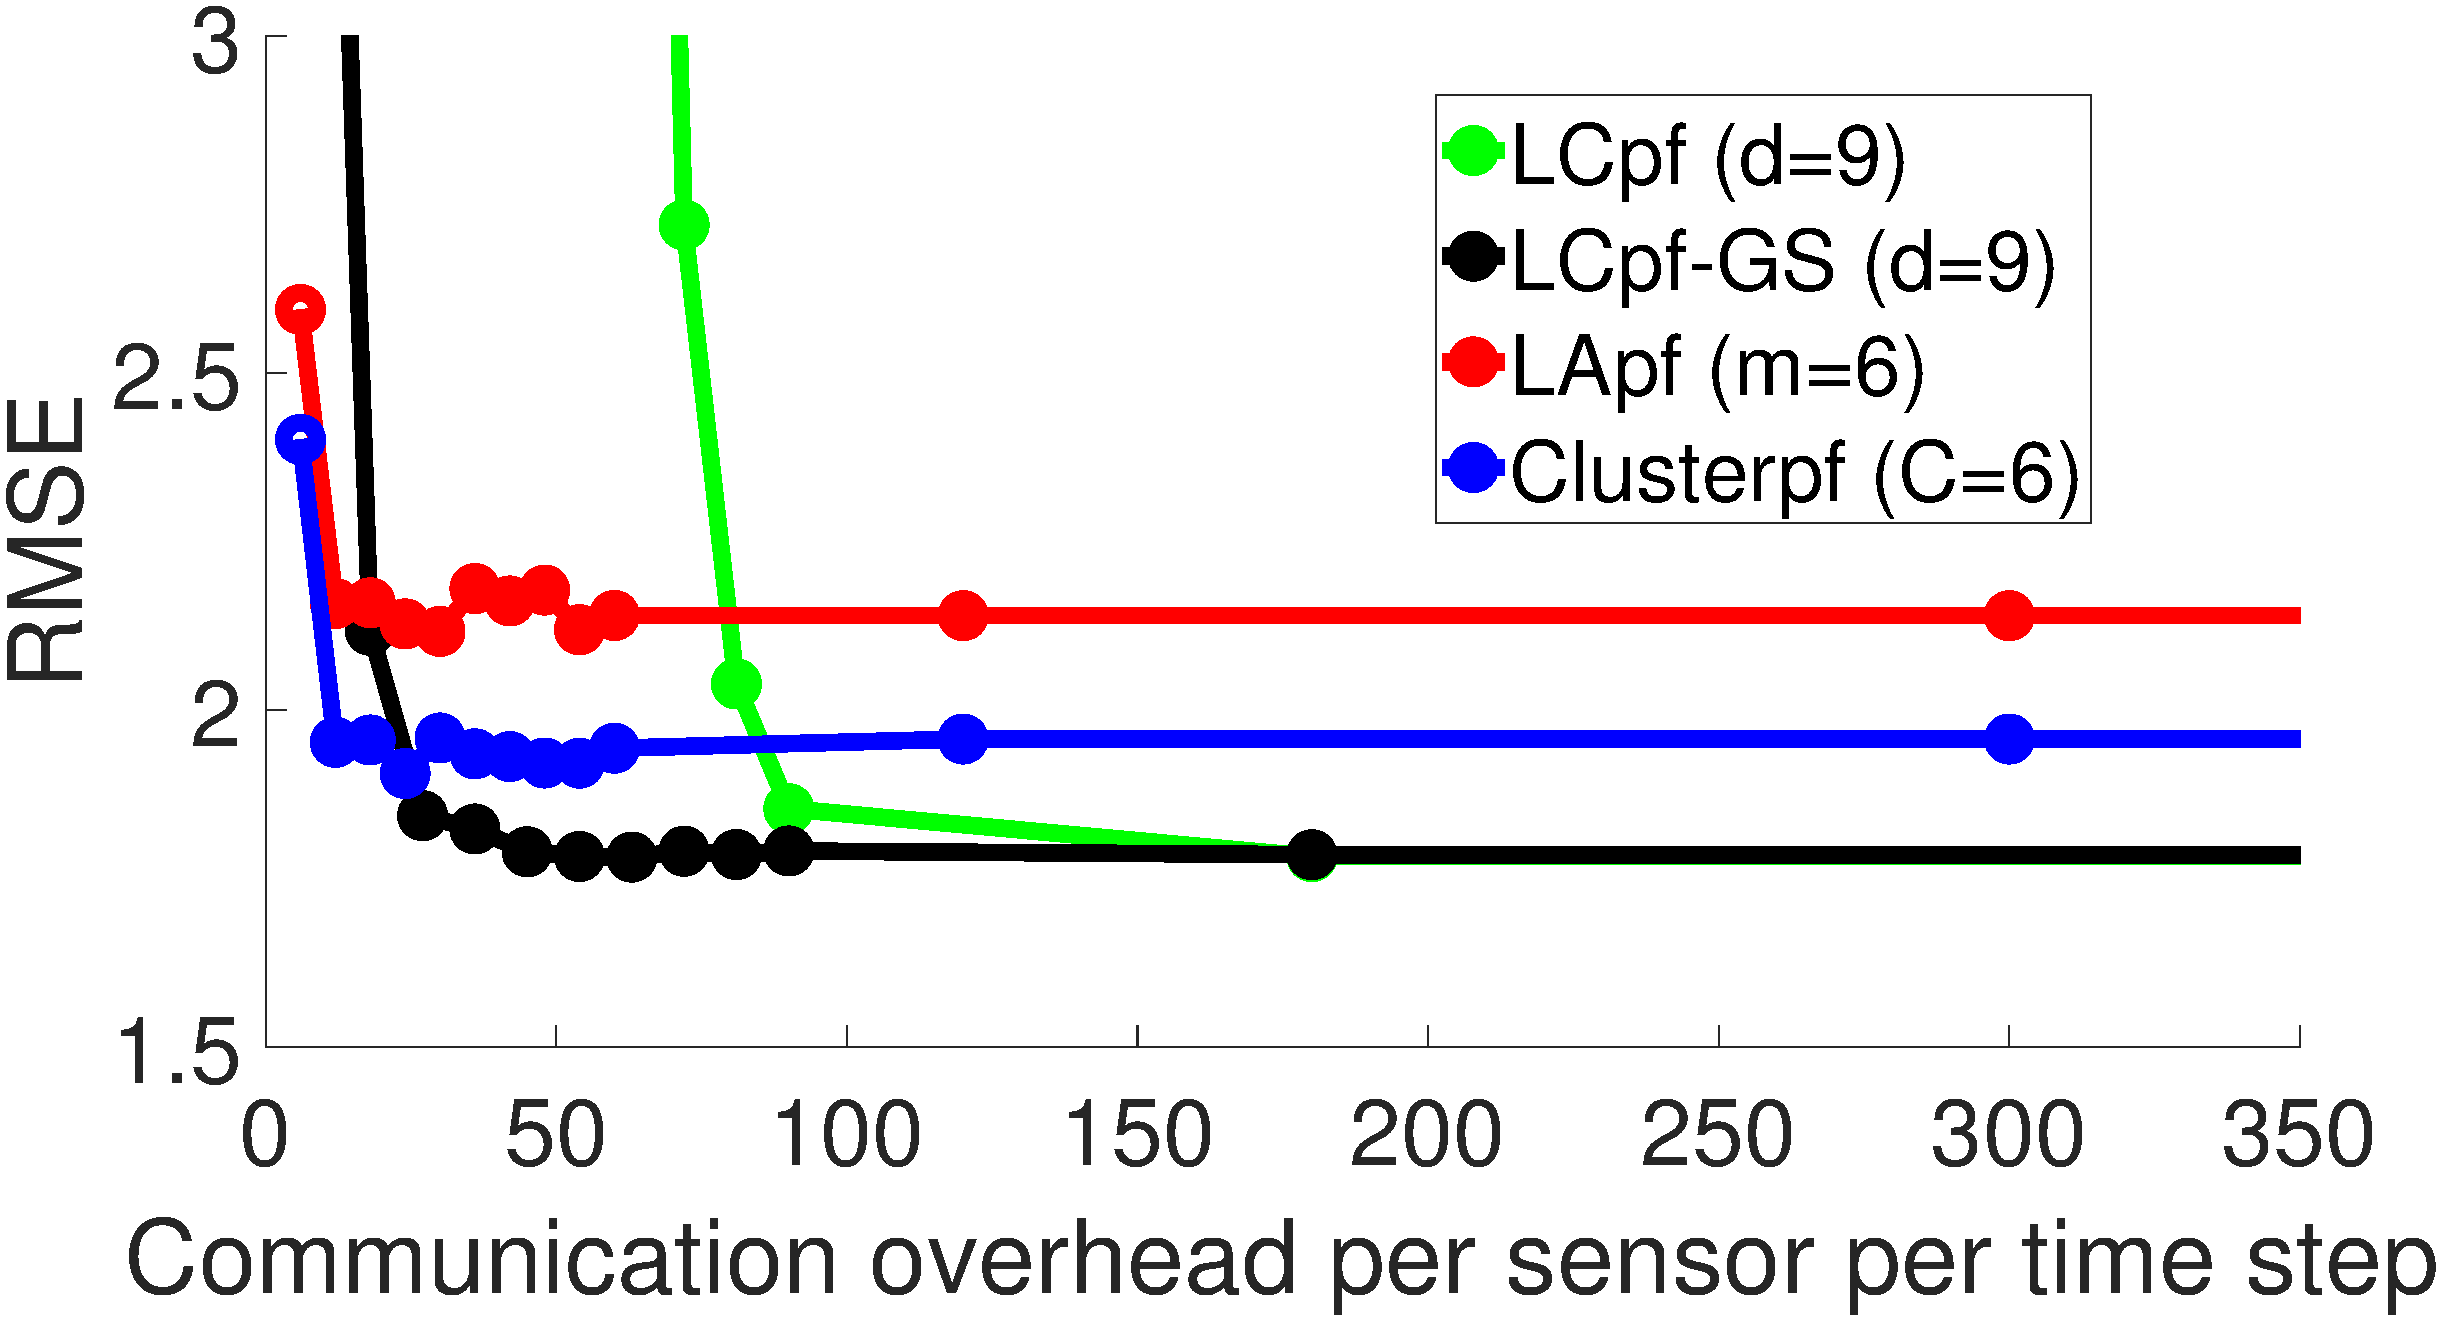
\includegraphics[width=0.75\textwidth]{Figures/Track1_range_RMSE}}
%\end{subfigure}
%\begin{subfigure}[Track 2]
%{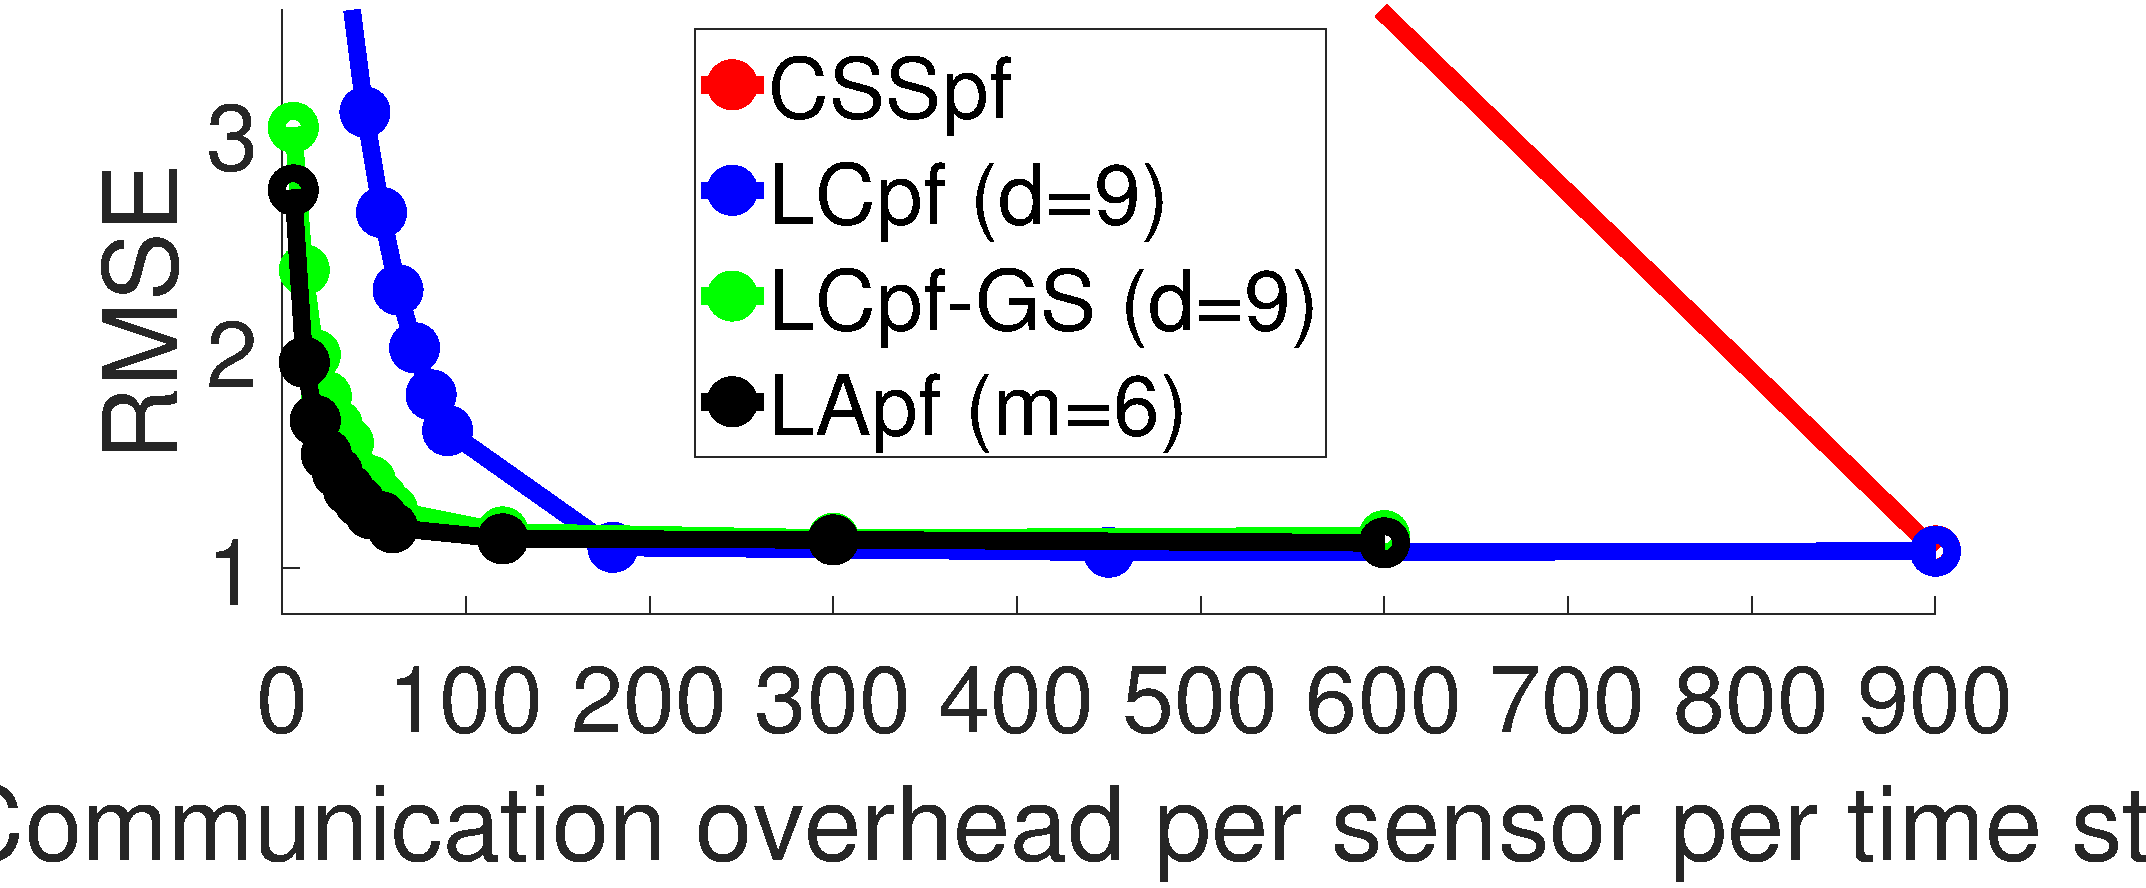
\includegraphics[width=0.75\textwidth]{Figures/Track2_range_RMSE}}
%\end{subfigure}
%\begin{subfigure}[Track 3]
%{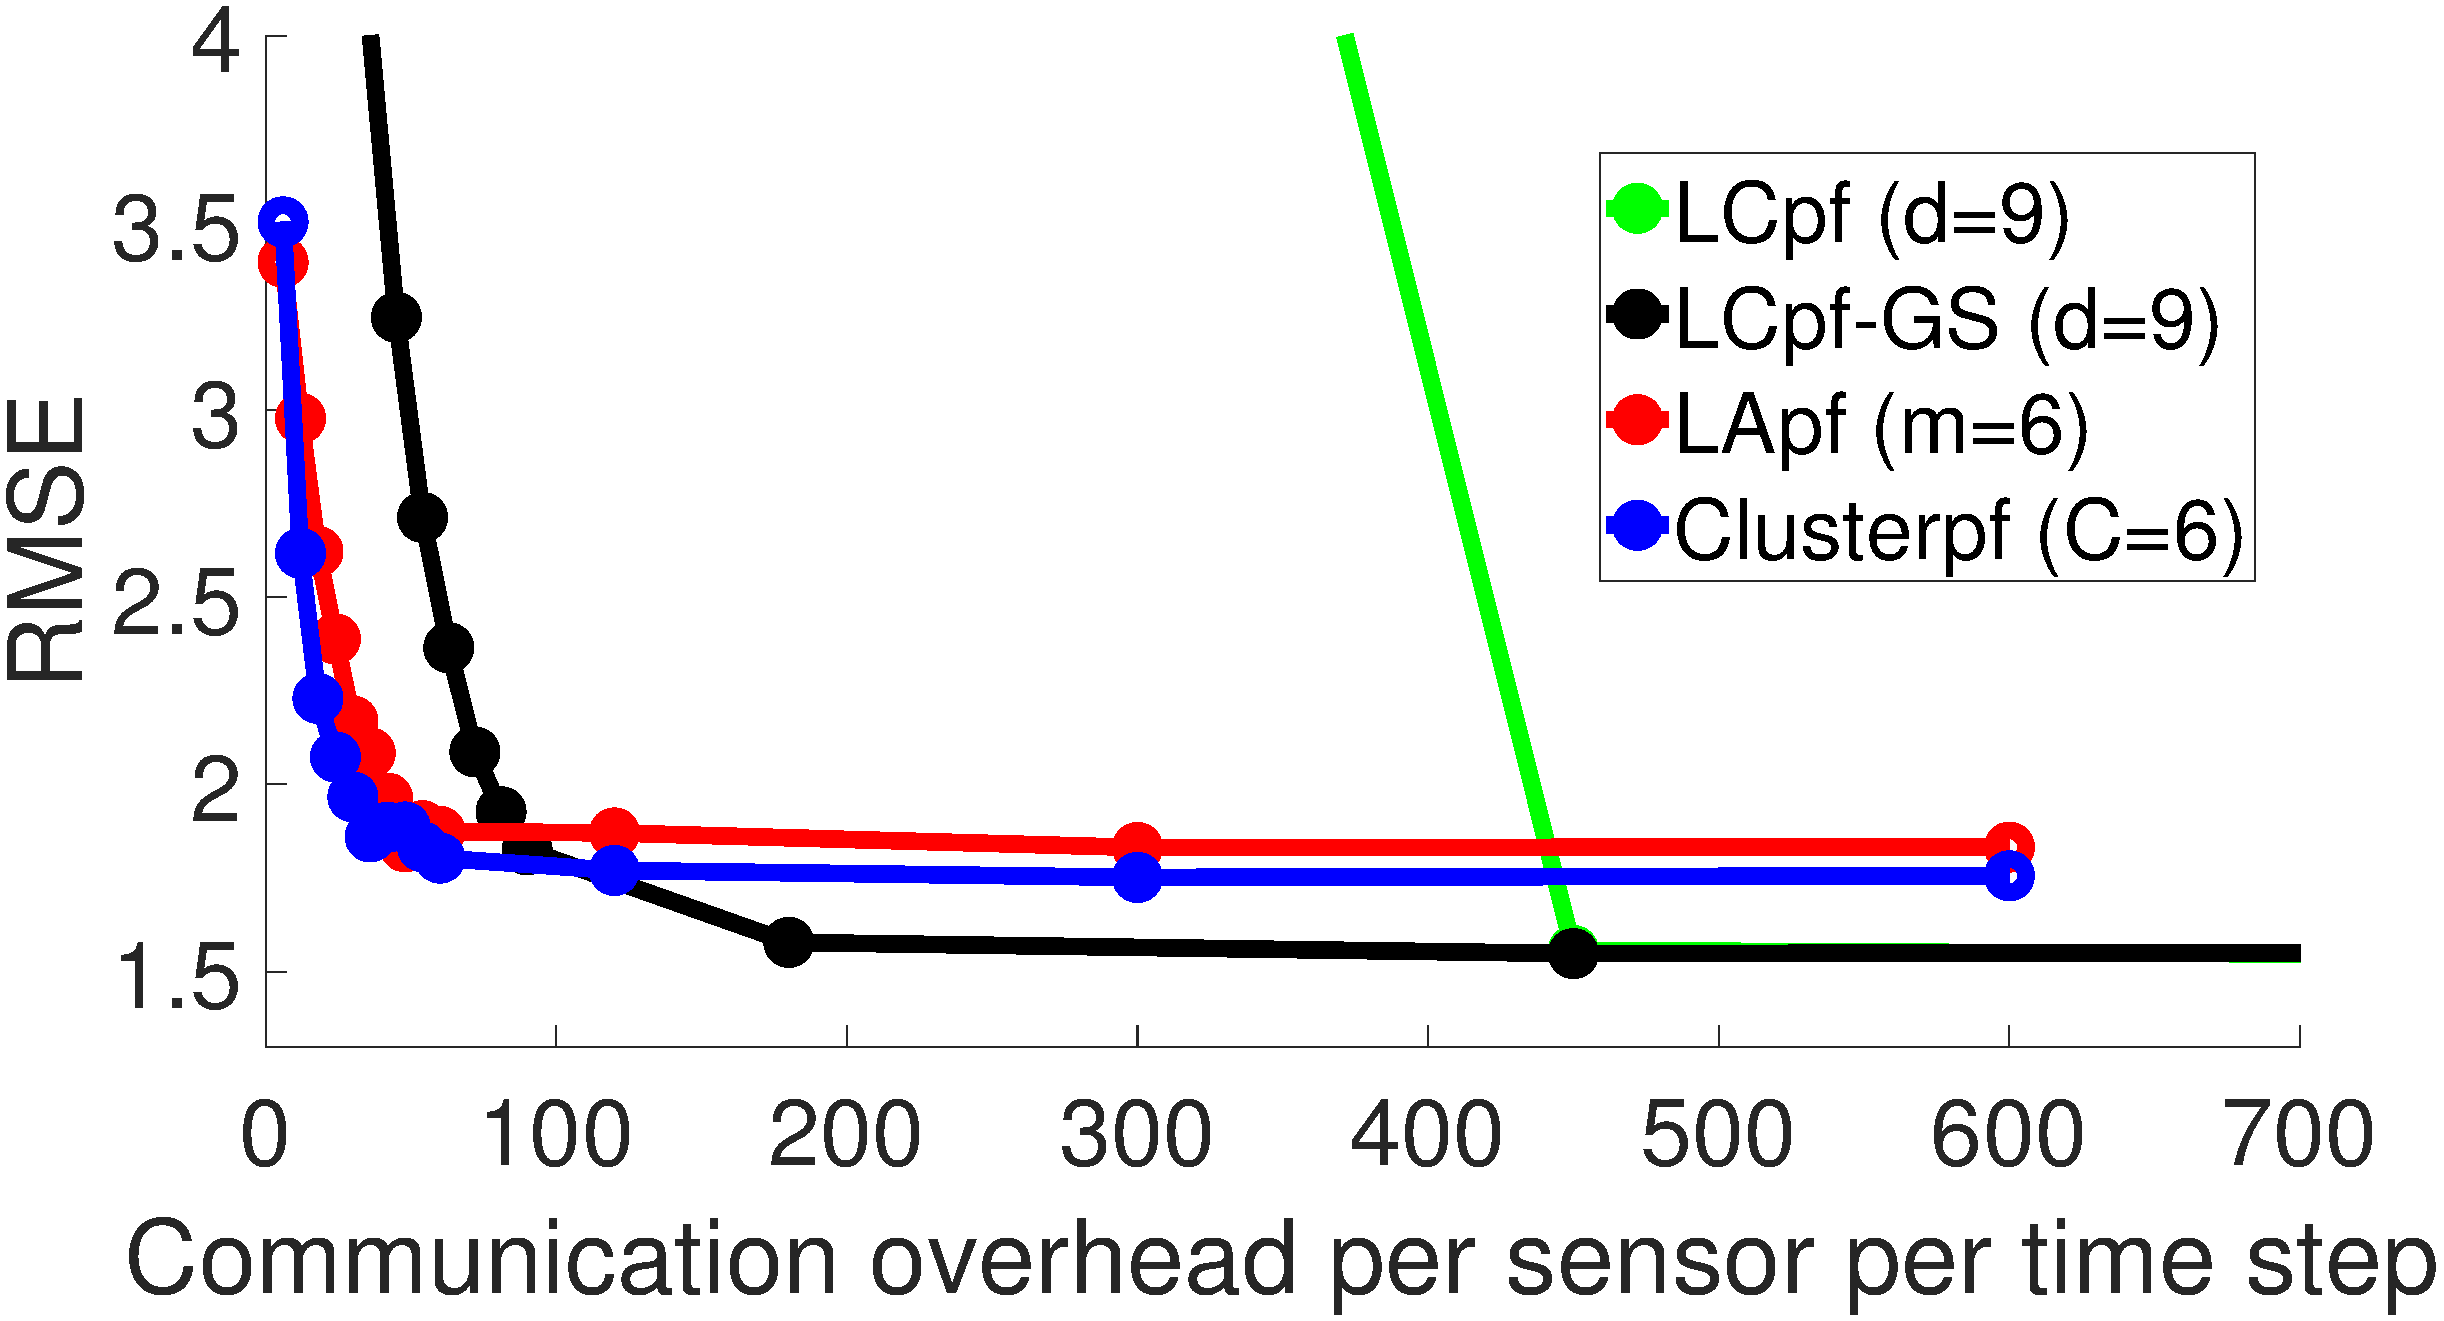
\includegraphics[width=0.75\textwidth]{Figures/Track3_range_RMSE}}
%\end{subfigure}
%\caption{Average RMSE with respect to total communication overhead per time step for track 2 ($N=500$, 200 Monte Carlo trials).}
%\label{fig:Track_range_results}
%\end{figure}
%

\section{Theoretical analysis}
All four filters encode the particle log-likelihoods in a similar fashion but yet display drastically different performance at low communication overhead. 

Let $\gamma_s$ denote the $N\times 1$ column vector of particle log-likelihoods at sensor $s$ and let $\gamma = \sum_{s=1}^S \gamma_s$ denote the joint log-likelihoods. Denote by $\Psi$ the $N\times J$ encoding matrix where $J \leq N$ is the number of encoding coefficients. In general, $\Psi$ is a function of local particles $x_i$. Finally, denote by $\alpha_s$ the $J\times 1$ column vector of encoded coefficients that capture all information at sensor $s$. 

For CSSpf, LCpf, LCpf-GS and LApf, the joint log-likelihoods are computed as follows:
\begin{align}
\alpha_s &= (\Psi^T \Psi)^{-1}\Psi^T \gamma_s\\
\alpha &= \sum_{s=1}^S \alpha_s = \sum_{s=1}^S (\Psi^T \Psi)^{-1}\Psi^T \gamma_s \\
\gamma &= \Psi \alpha = \Psi \sum_{s=1}^S (\Psi^T \Psi)^{-1}\Psi^T \gamma_s
\end{align}

For Clusterpf, the vector $\gamma_s$ instead denotes the $C\times 1$ column vector of cluster log-likelihoods at sensor $s$. After the joint cluster log-likelihoods $\gamma$ are computed, individual particle log-likelihoods are recovered via convex optimization. This last step renders the analysis of Clusterpf more complicated and we omit all discussions related to Clusterpf for now. 

With low communication overhead, the gossip algorithm does not converge and all sensors obtain $\alpha' = \alpha + \Delta$. This yields
\begin{equation}
\gamma' = \Psi \alpha' = \Psi \alpha + \Psi \Delta
\end{equation}
where the term $\Psi \Delta$ induces error in the joint log-likelihoods. Taking the exponential yields
\begin{equation}
w = \exp(\gamma') = \exp(\Psi\alpha)\exp(\Psi\Delta)
\end{equation}
where the term $\exp(\Psi\Delta)$ is the distortion induced on (unnormalized) particle weights. 

In the ideal case, the gossip algorithm converges, $\Delta = 0$, and we have $\exp(\Psi \Delta)=\textbf{1}$ where $\textbf{1}$ is the vector of all 1's. In our perturbation test (Fig.~\ref{fig:perturbation_results}), we compute and report $\frac{1}{N}||\textbf{1}-\exp(\Psi \Delta)||_1$. For each filter, we compute the $N\times 1$ vector $\textbf{1}-\exp(\Psi \Delta)$ and report its average over $N$ particles. A value closer to 0 indicates less distortion to the particle weights due to gossiping error. Conversely, a value close to 1 indicates high distortion. Fig.~\ref{fig:perturbation_expPsiDelta} shows the results for all three tracks. In all perturbation tests, LApf has the lowest curve, followed by LCpf-GS and Clusterpf. LCpf has the highest curve for all perturbation levels. On the other hand, in the NGossip tests, Clusterpf and LApf have very similar level distortions. These trends are consistent with Fig.~\ref{fig:perturbation_results} which shows the discrepancy in normalized particle weights estimation. These results are also consistent with our previous observation that LApf and Clusterpf have robust performance even at low communication overhead.

\begin{figure}
\centering
\begin{subfigure}[Track 1]
{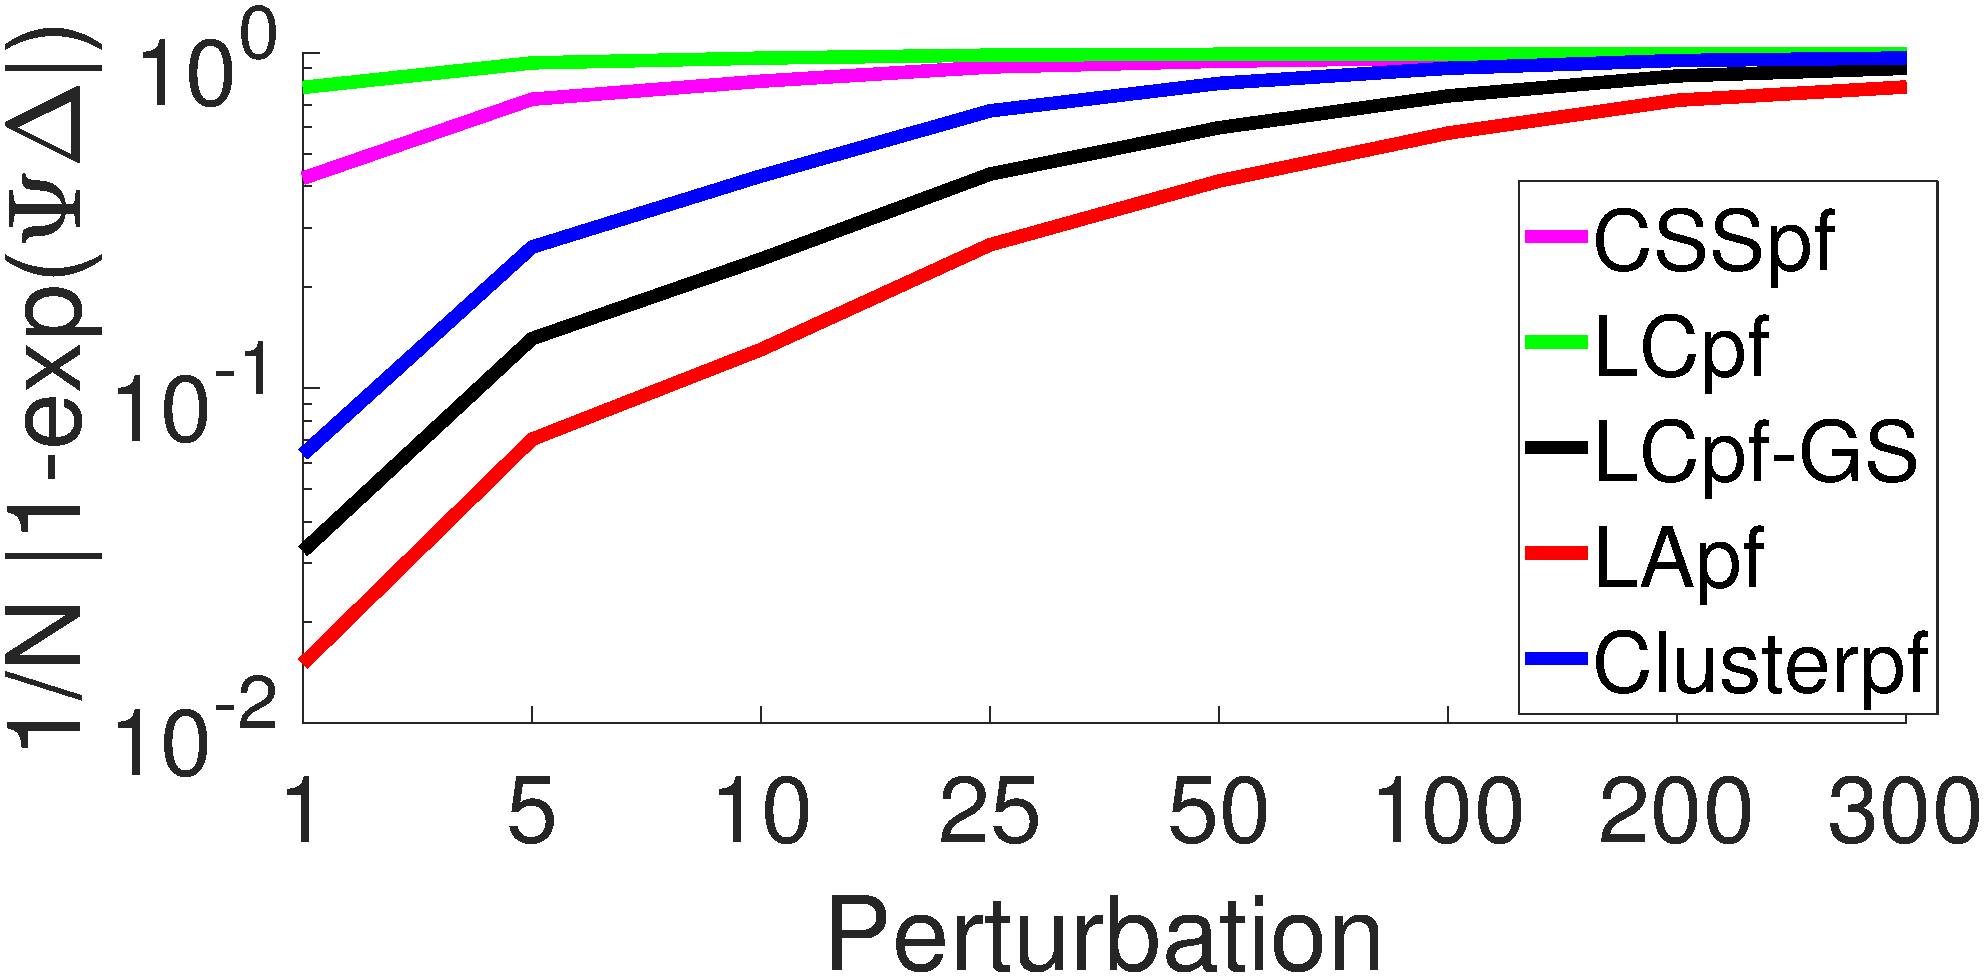
\includegraphics[width=0.49\textwidth]{Figures/expPsiDelta_track1}}
\end{subfigure}
\begin{subfigure}[Track 1]
{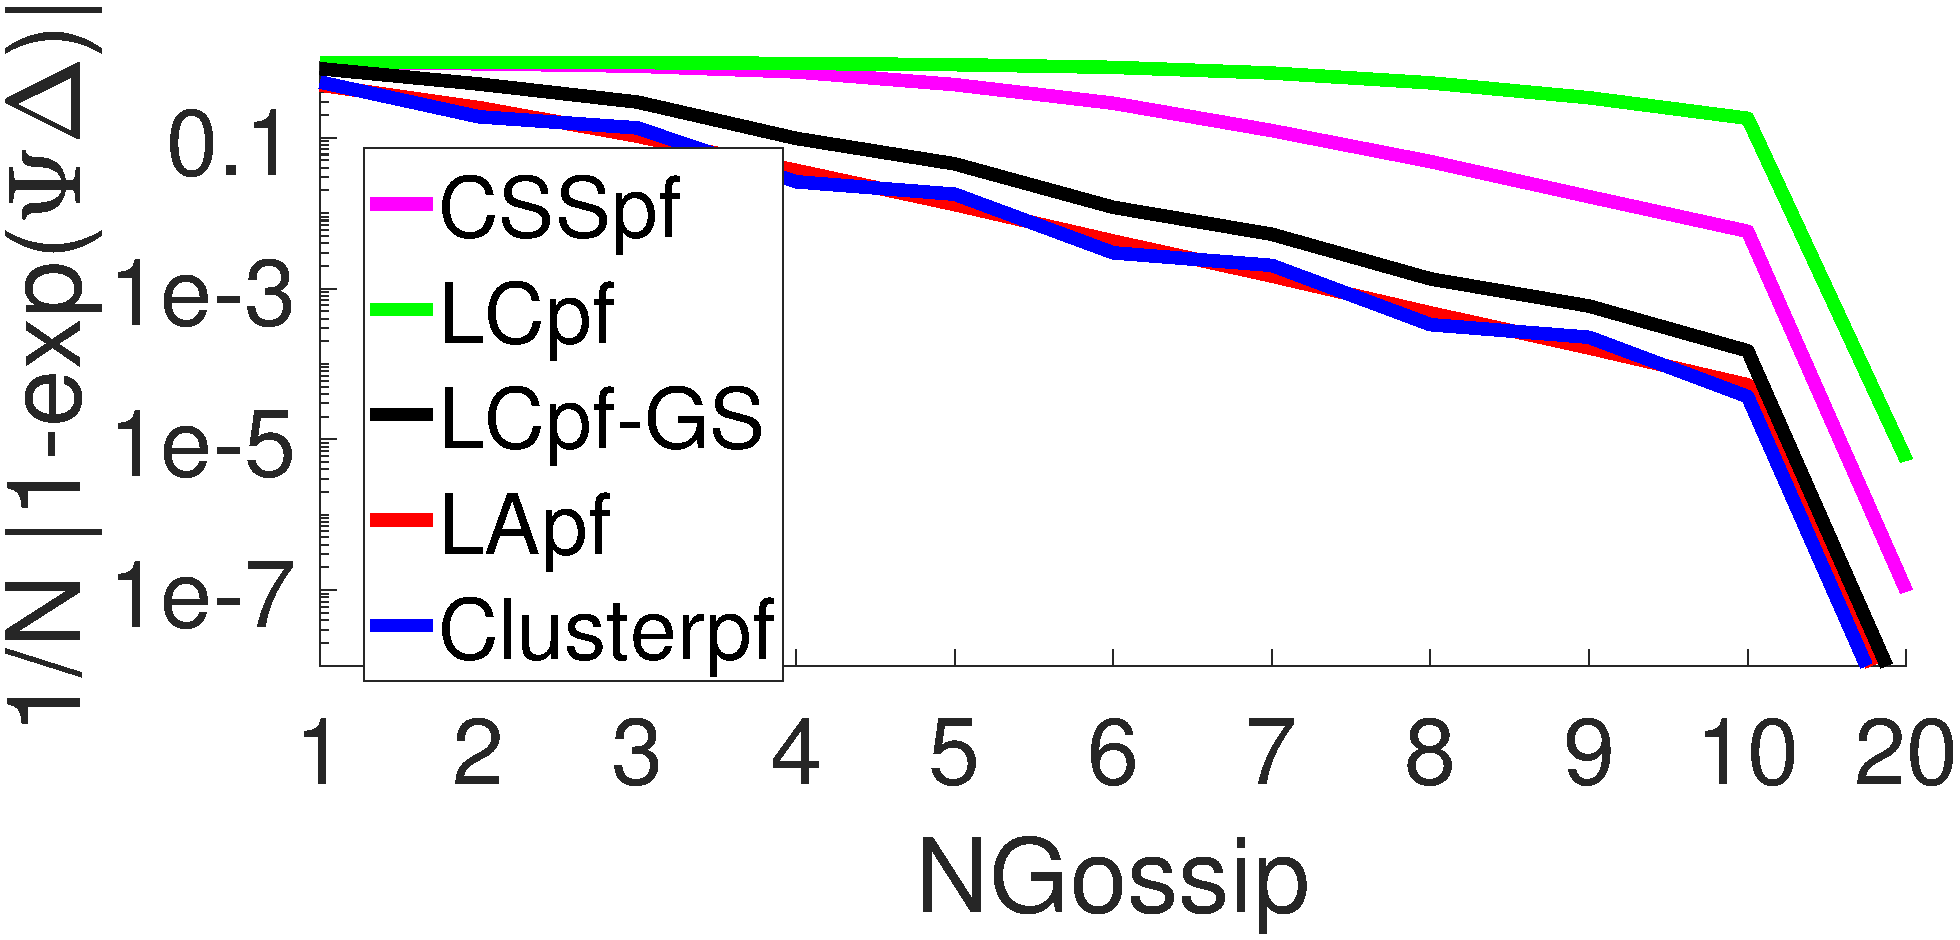
\includegraphics[width=0.49\textwidth]{Figures/expPsiDelta_Gossip_track1}}
\end{subfigure}
\begin{subfigure}[Track 2]
{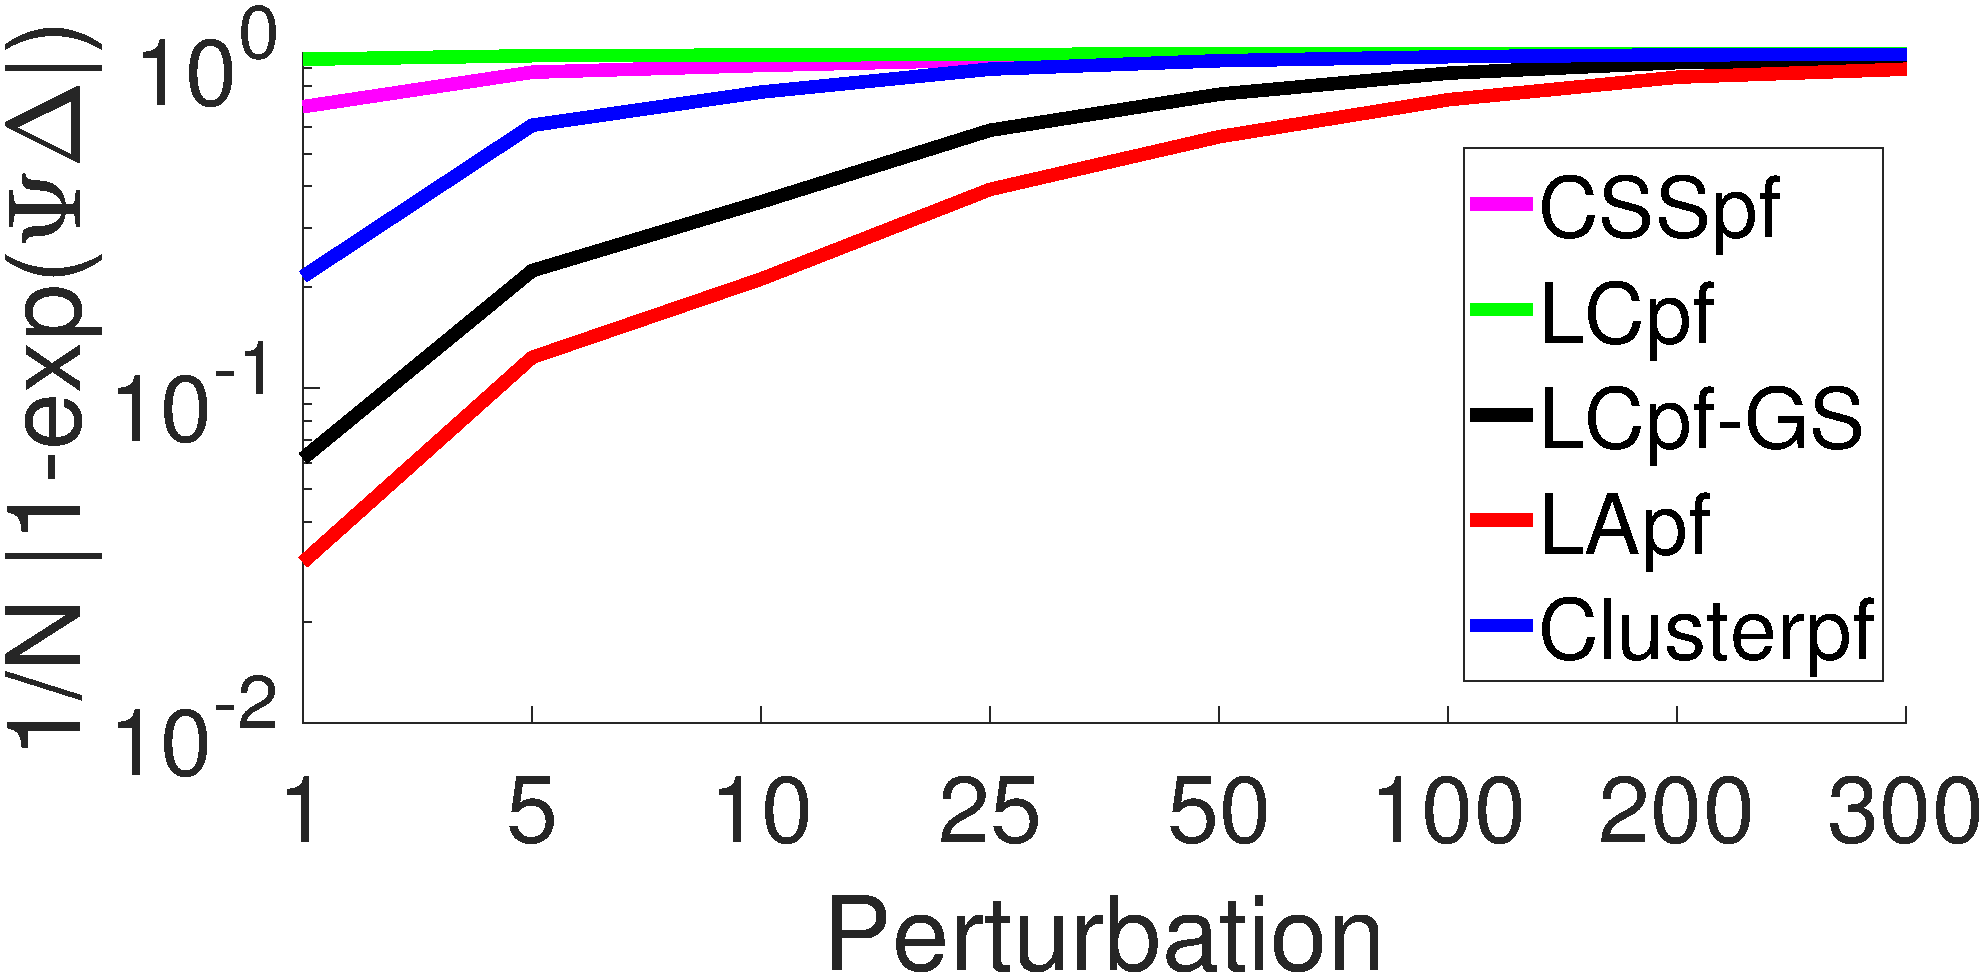
\includegraphics[width=0.49\textwidth]{Figures/expPsiDelta_track2}}
\end{subfigure}
\begin{subfigure}[Track 2]
{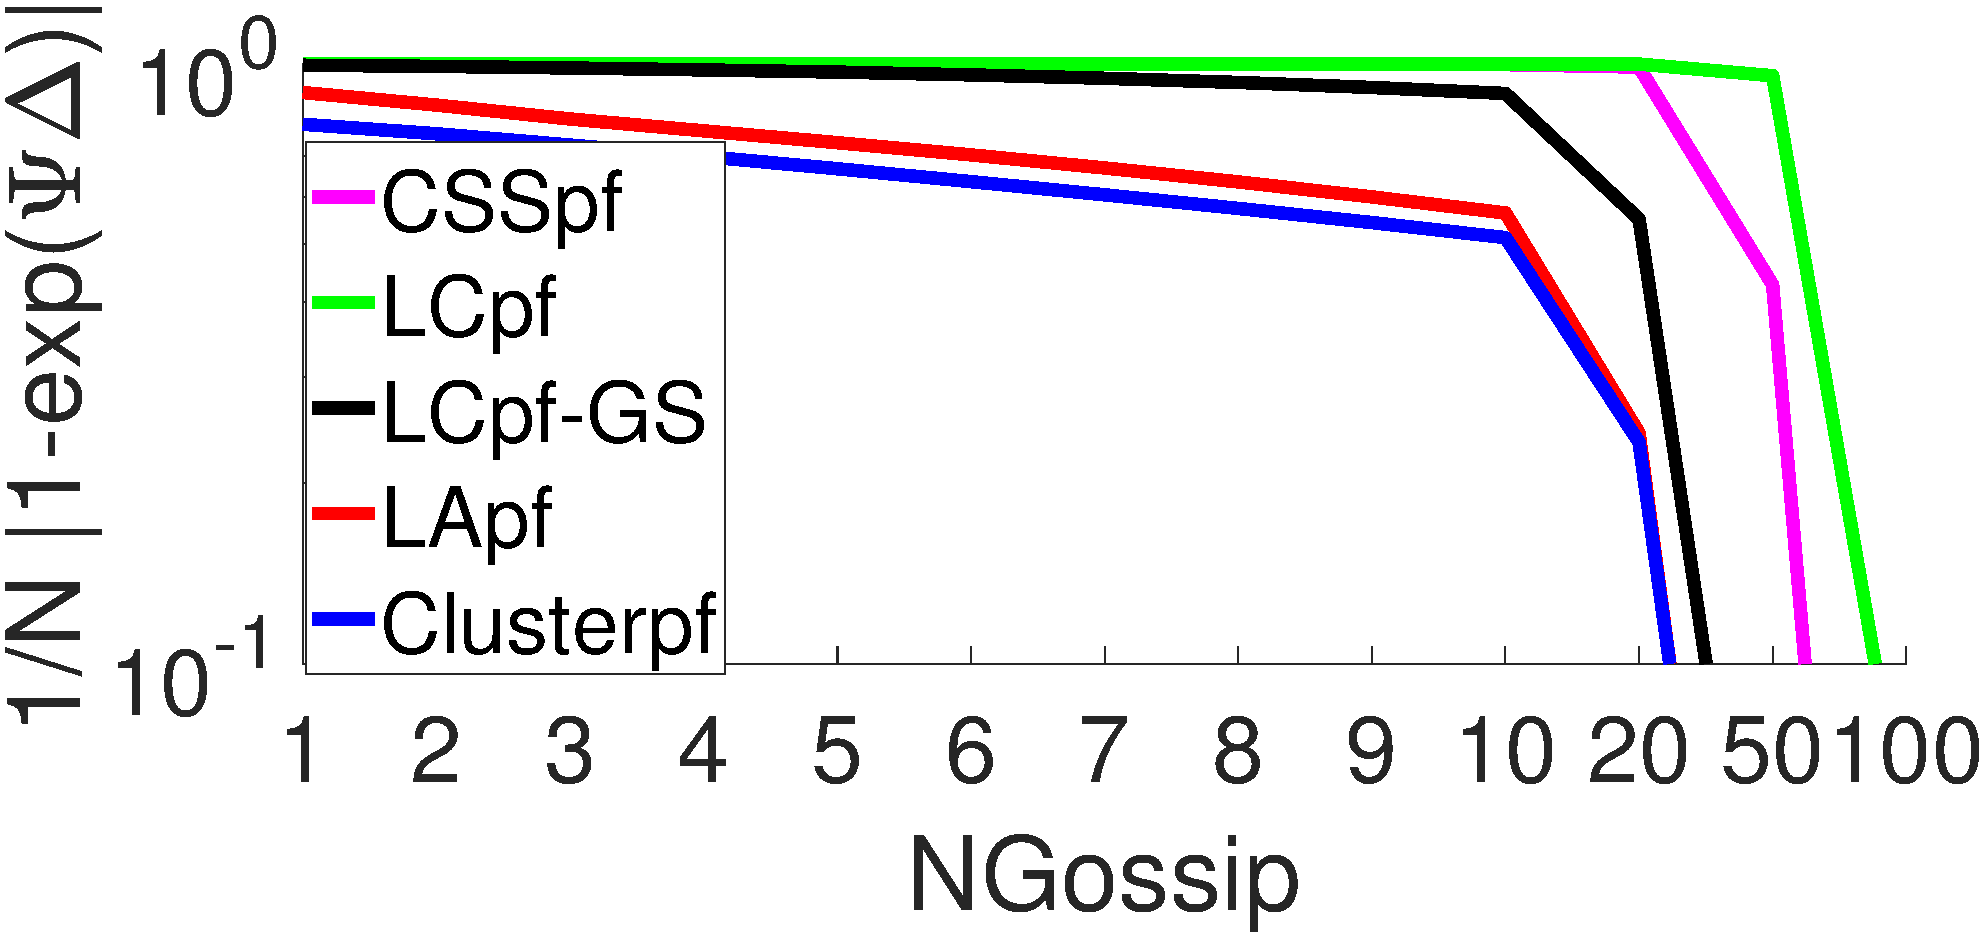
\includegraphics[width=0.49\textwidth]{Figures/expPsiDelta_Gossip_track2}}
\end{subfigure}
\begin{subfigure}[Track 3]
{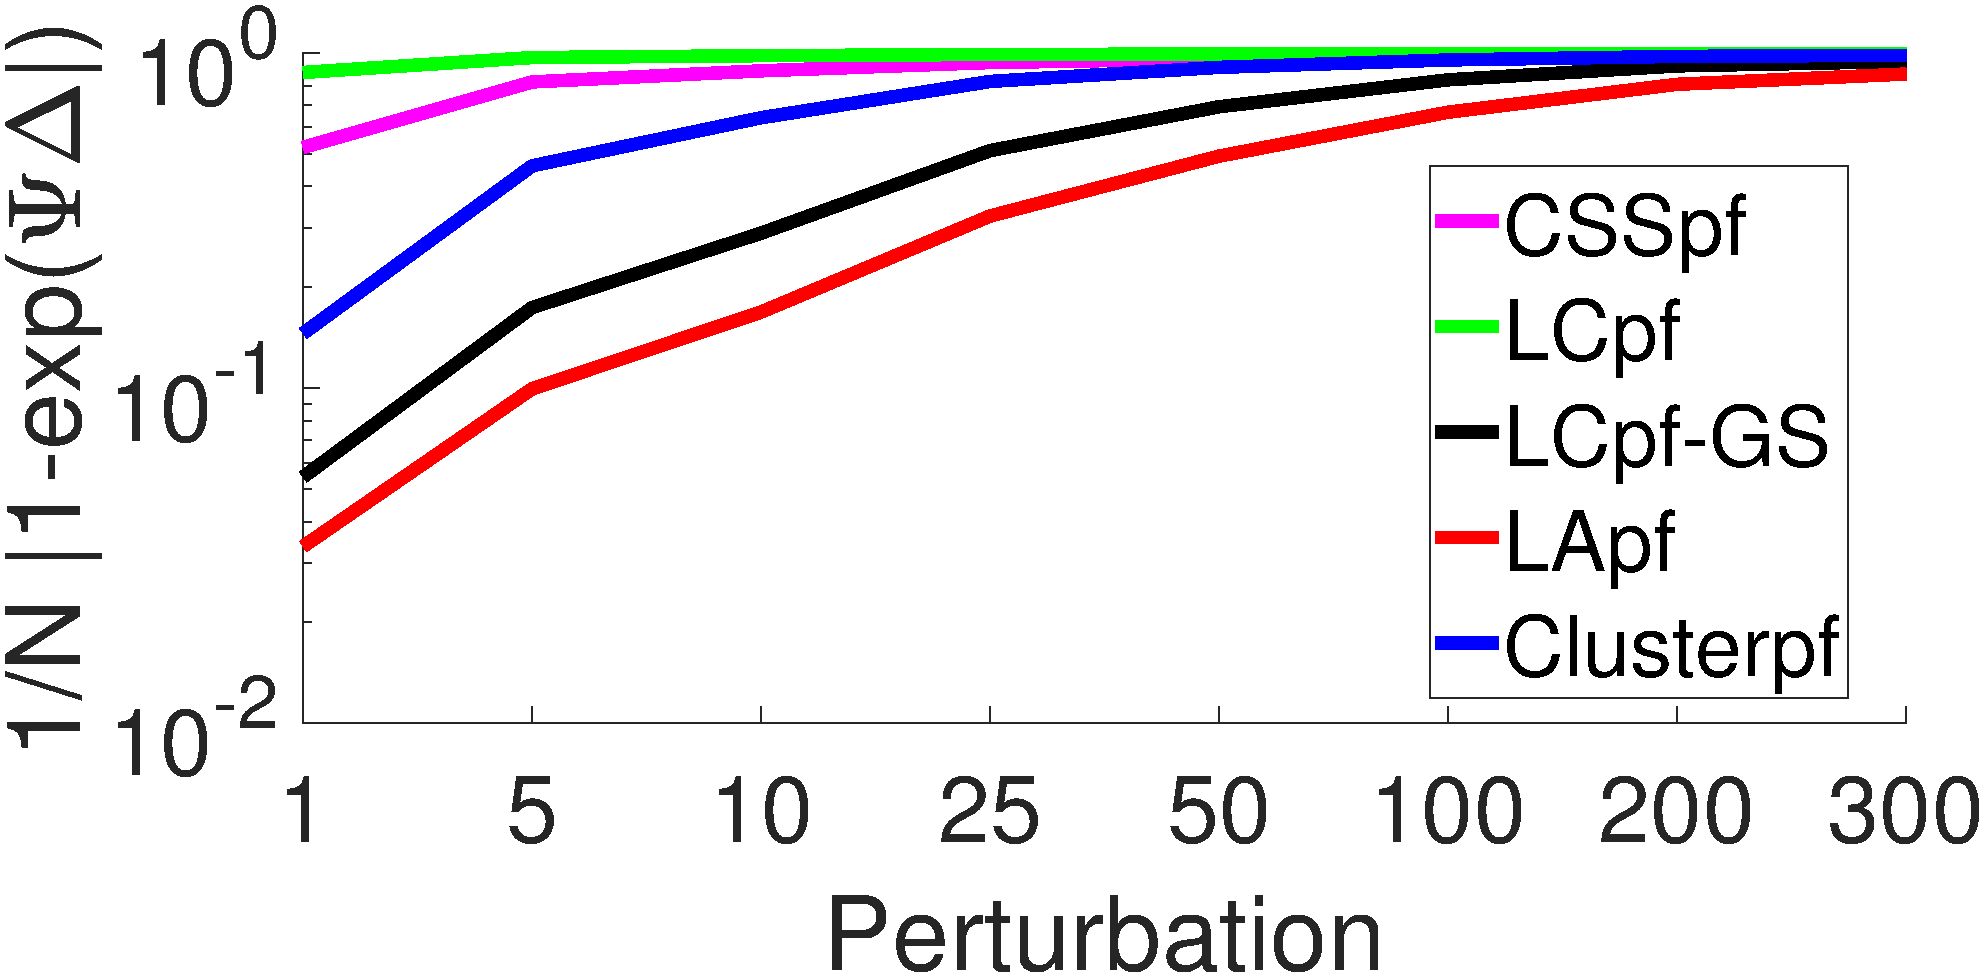
\includegraphics[width=0.49\textwidth]{Figures/expPsiDelta_track3}}
\end{subfigure}
\begin{subfigure}[Track 3]
{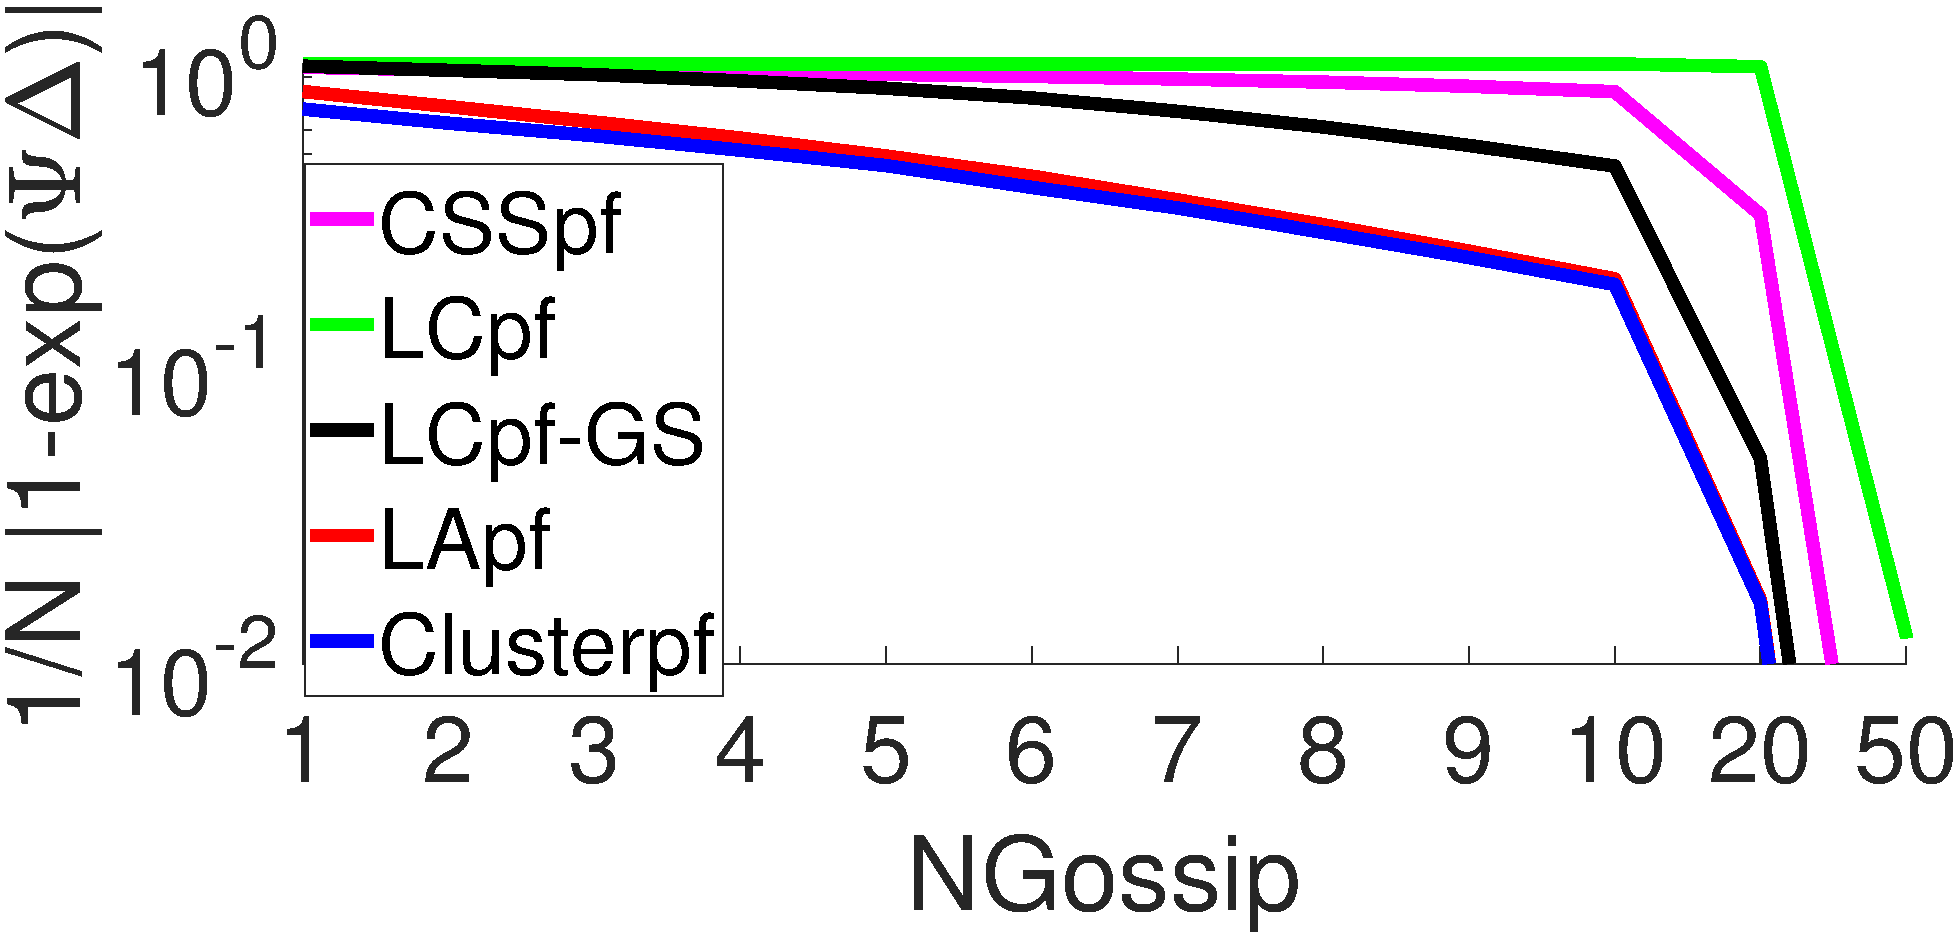
\includegraphics[width=0.49\textwidth]{Figures/expPsiDelta_Gossip_track3}}
\end{subfigure}
\caption{Average value of $\textbf{1}-\exp(\Psi\Delta)$ over $N$ particles. A perturbation of $x$ represents $x\%$ shift from the true aggregate value. $N=500$, $d=1,m=C=6$}
\label{fig:perturbation_expPsiDelta}
\end{figure}

Fig.~\ref{fig:perturbation_PsiDelta} shows the average $||\Psi \Delta||_w$ for all filters on all three tracks. The distortion increases at higher perturbation level and decreases with higher NGossip as expected. LApf, Clusterpf and LCpf-GS have similar level of distortion for all NGossip values. 

\begin{figure}
\centering
\begin{subfigure}[Track 1]
{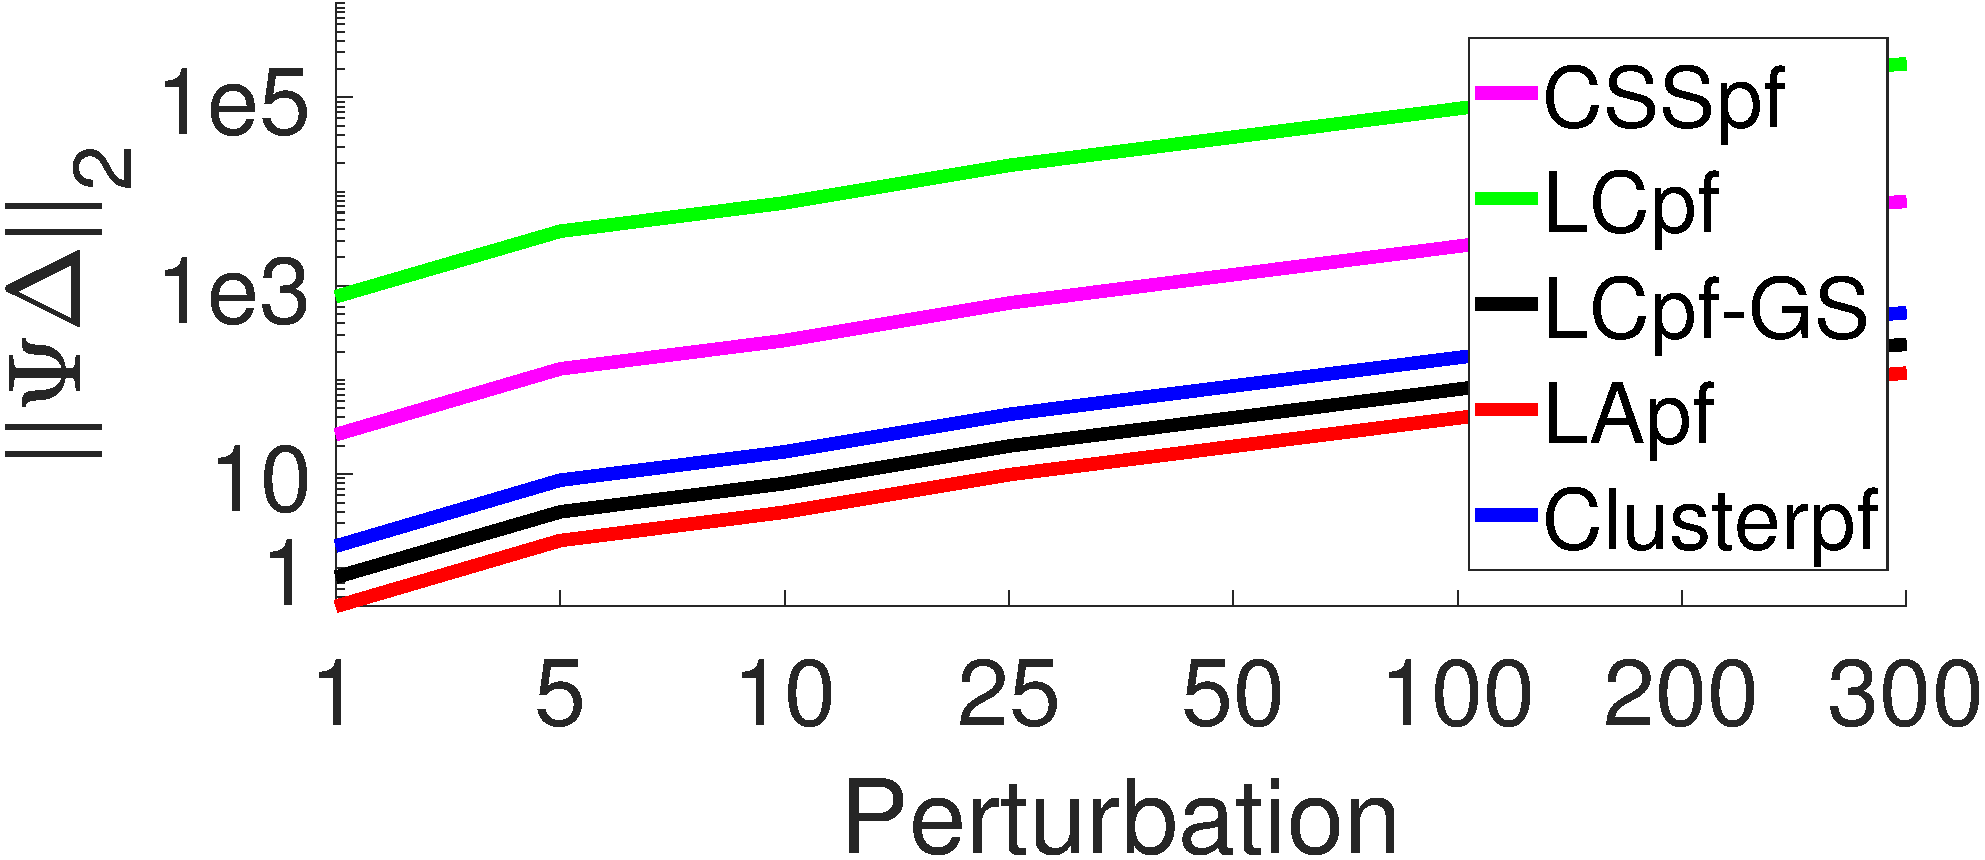
\includegraphics[width=0.49\textwidth]{Figures/PsiDelta_track1}}
\end{subfigure}
\begin{subfigure}[Track 1]
{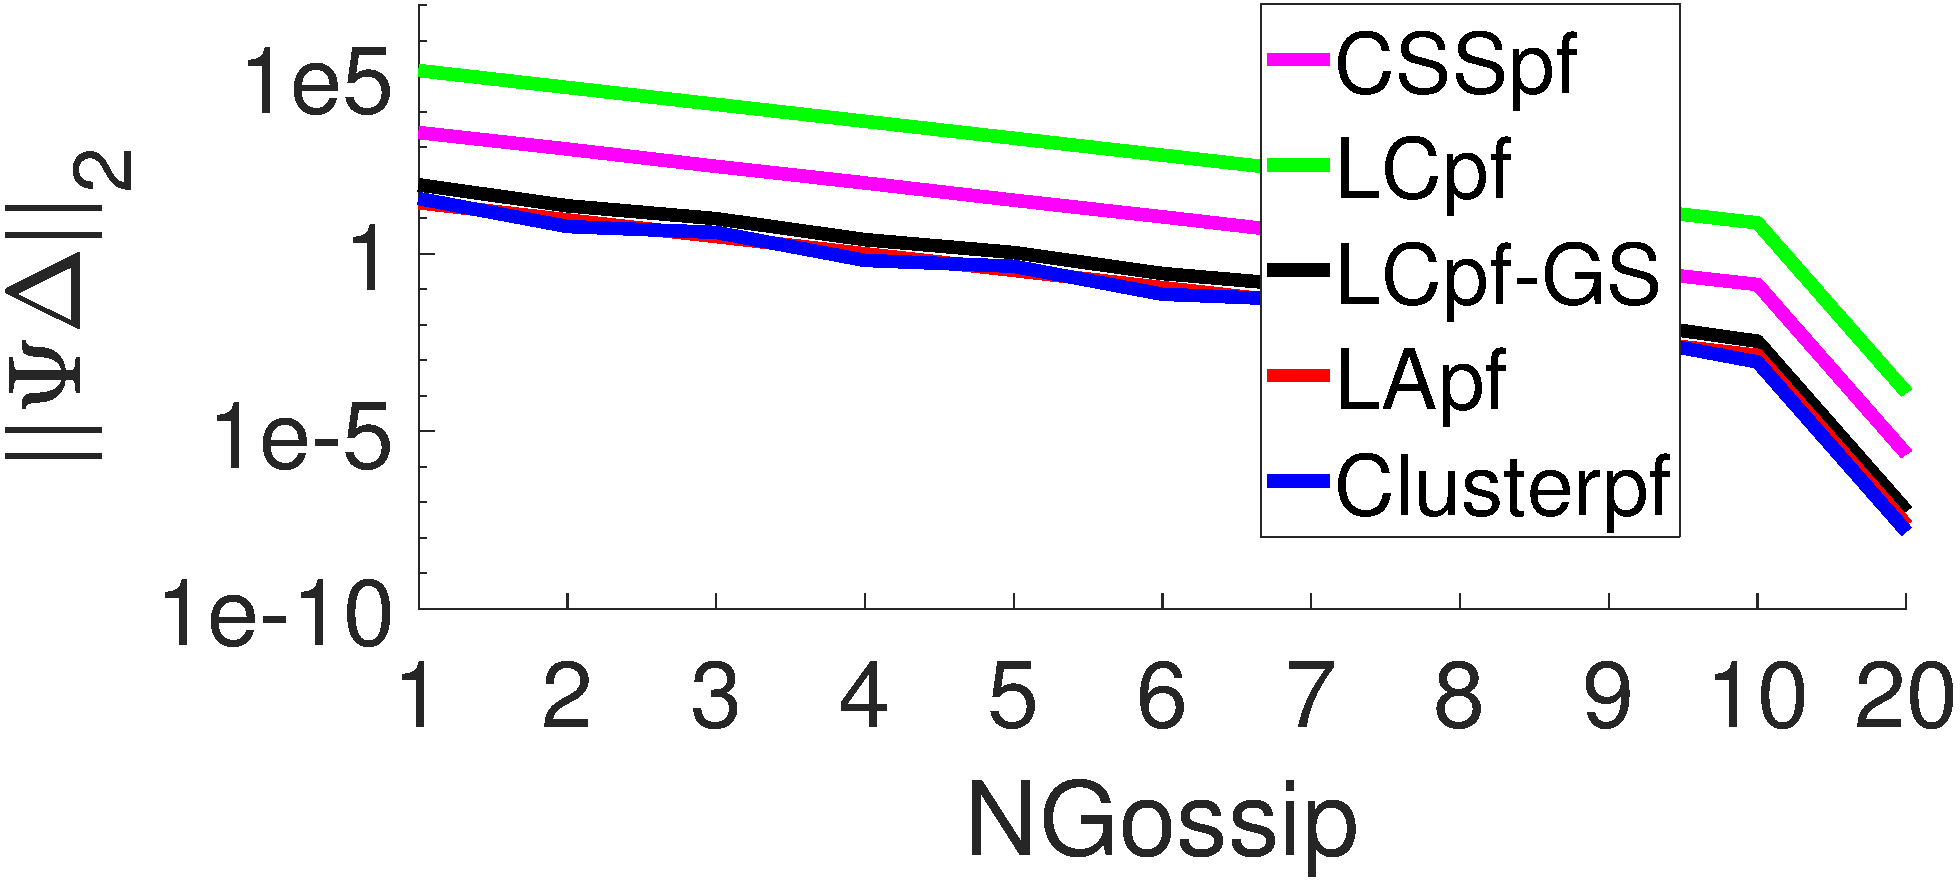
\includegraphics[width=0.49\textwidth]{Figures/PsiDelta_Gossip_track1}}
\end{subfigure}
\begin{subfigure}[Track 2]
{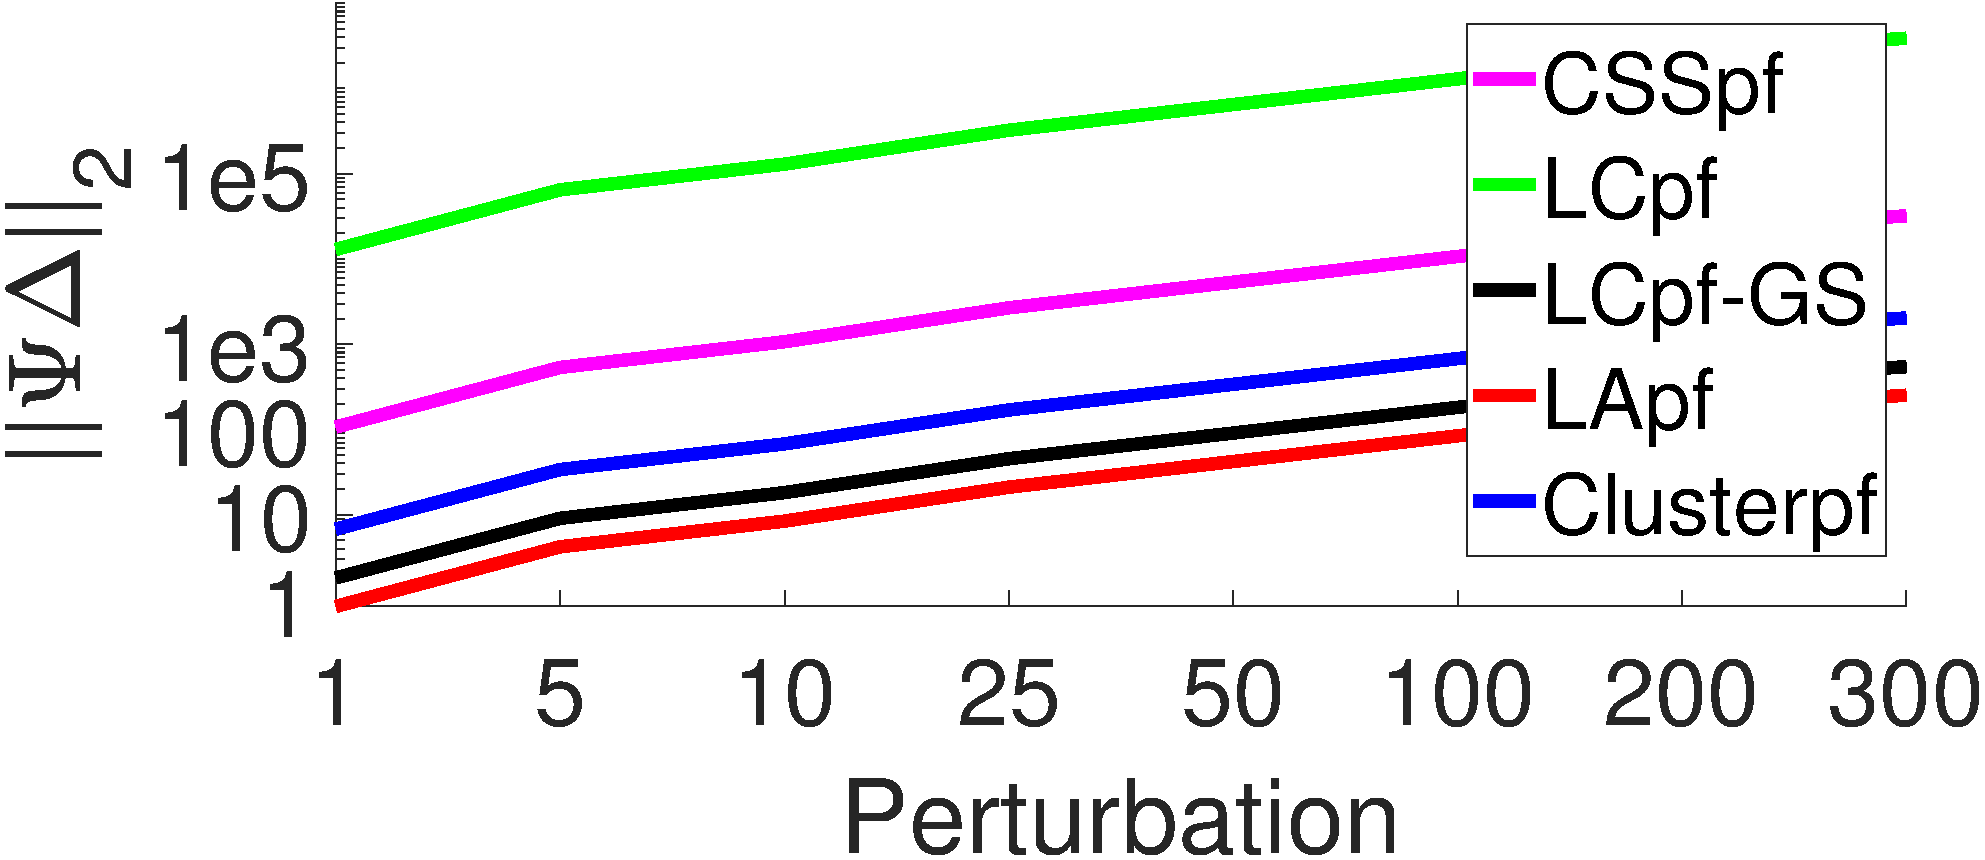
\includegraphics[width=0.49\textwidth]{Figures/PsiDelta_track2}}
\end{subfigure}
\begin{subfigure}[Track 2]
{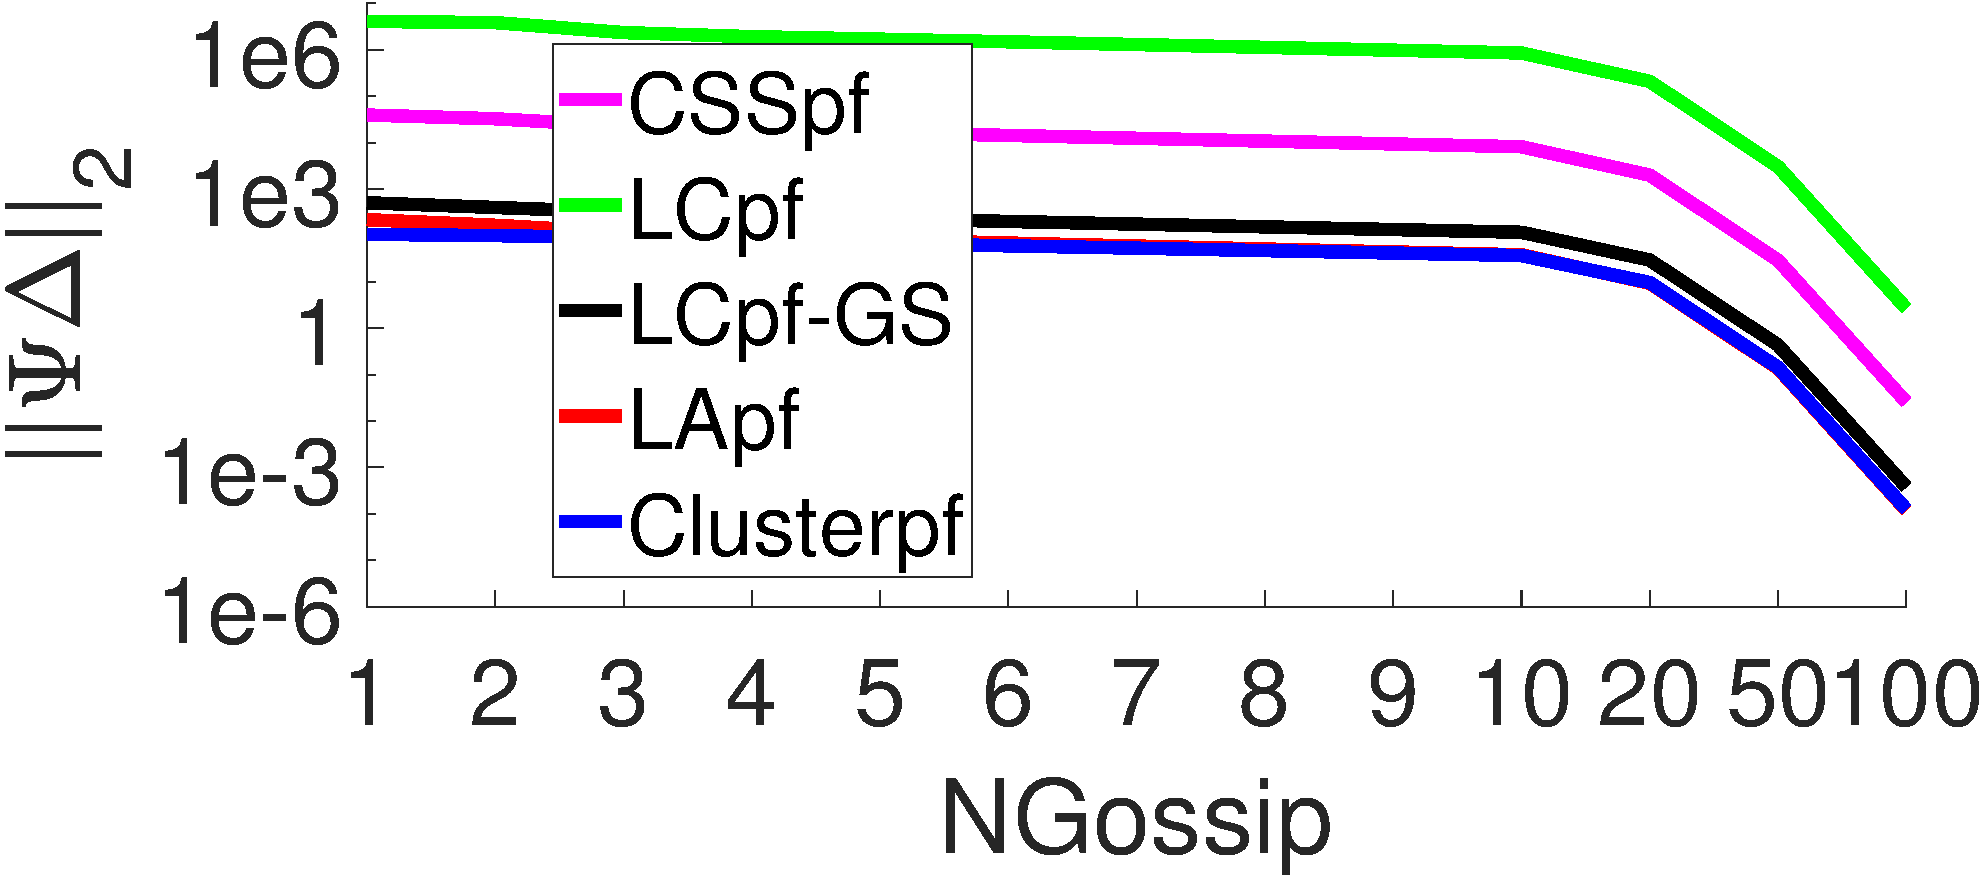
\includegraphics[width=0.49\textwidth]{Figures/PsiDelta_Gossip_track2}}
\end{subfigure}
\begin{subfigure}[Track 3]
{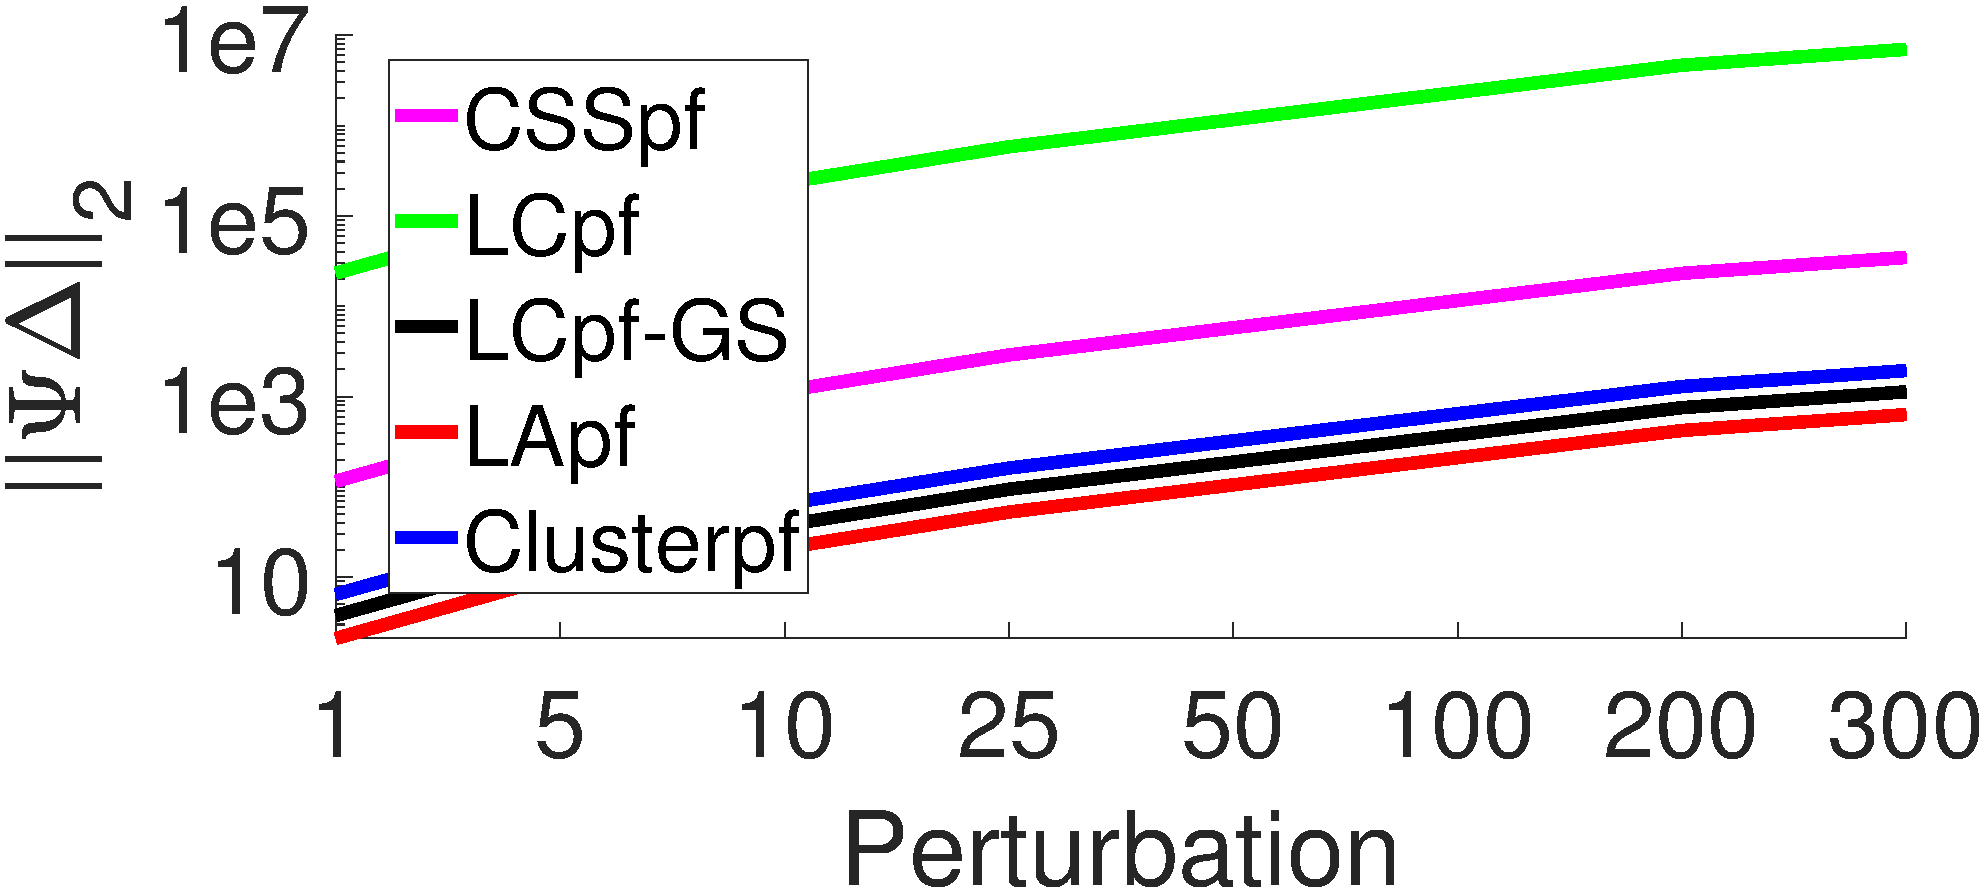
\includegraphics[width=0.49\textwidth]{Figures/PsiDelta_track3}}
\end{subfigure}
\begin{subfigure}[Track 3]
{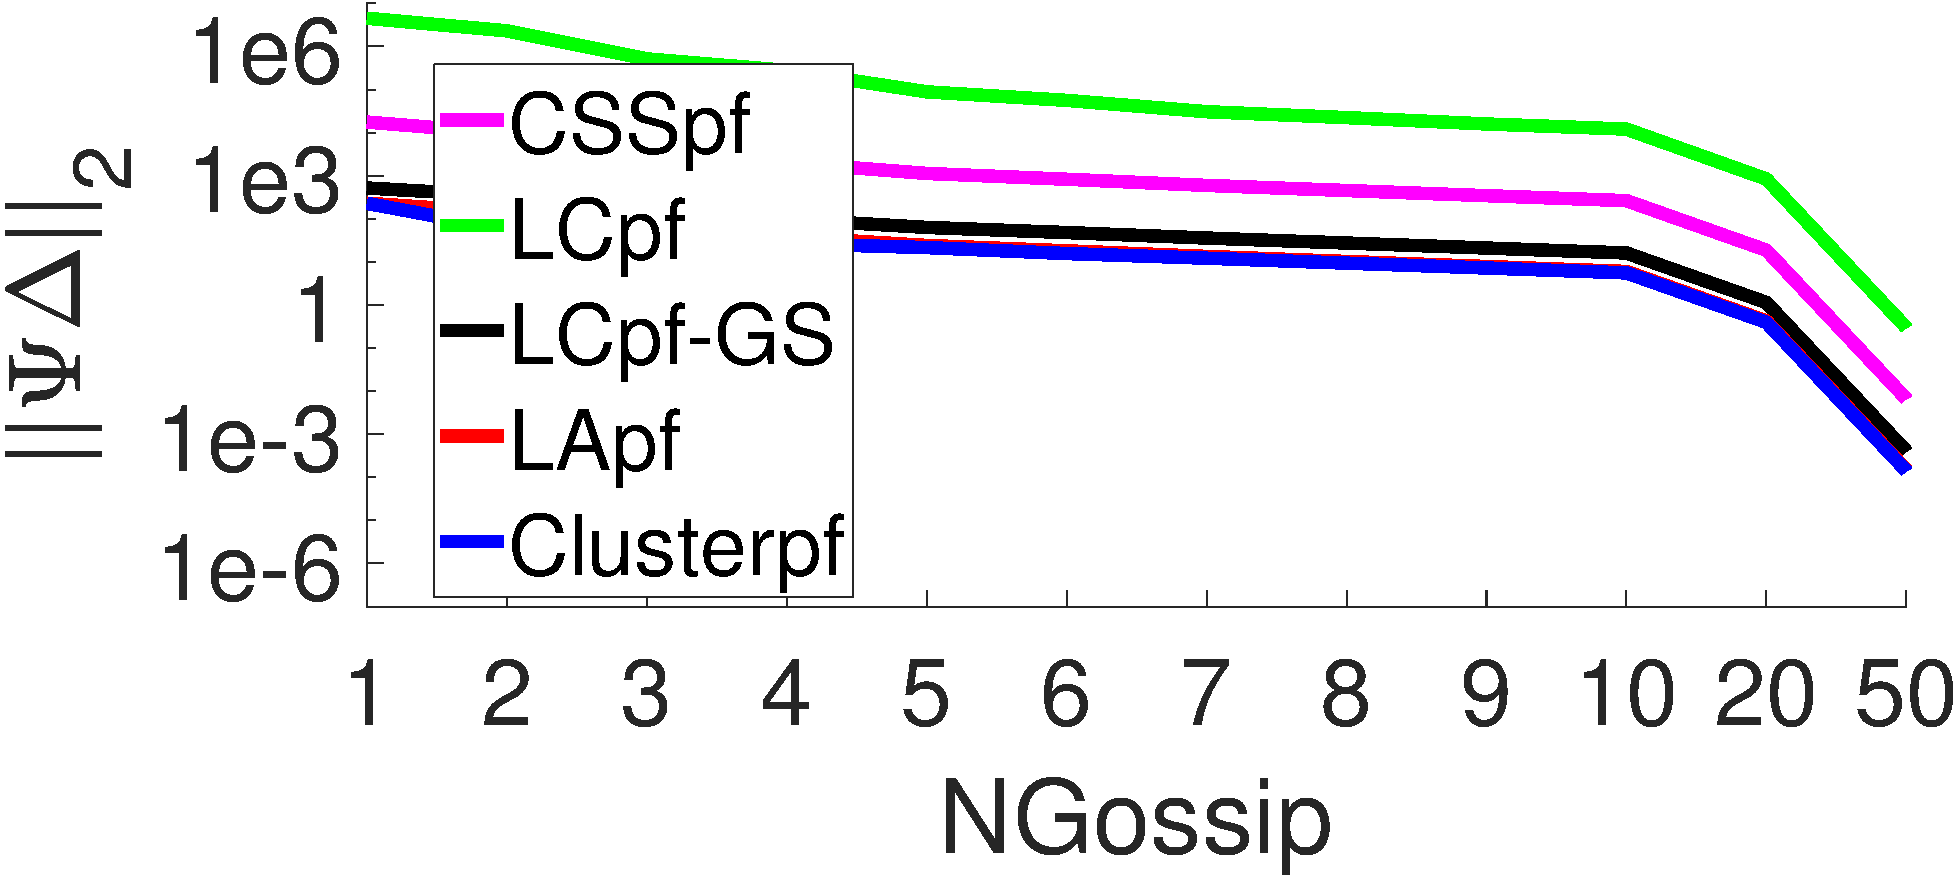
\includegraphics[width=0.49\textwidth]{Figures/PsiDelta_Gossip_track3}}
\end{subfigure}
\caption{Average value of $||\Psi\Delta||_2$. A perturbation of $x$ represents $x\%$ shift from the true aggregate value. $N=500$, $d=1,m=C=6$}
\label{fig:perturbation_PsiDelta}
\end{figure}

Our objective is to derive some suitable bounds on the distortion $||\Psi \Delta||$. From the submultiplicative property of $L_2$ norm, we have
\begin{equation}
||\Psi \Delta|| \leq ||\Psi|| \cdot ||\Delta||
\end{equation}

For LCpf-GS and LApf, the encoding matrices are orthonormal and thus have norm 1. On the other hand, $||\Psi_{CSS}||$ and $||\Psi_{LC}||$ depend strongly on the states of particles $x_i$ and the choice of basis functions.

We seek to bound the gossip error $||\Delta||$. Let $W$ denote the mixing matrix in the gossip algorithm. Let $k$ denote the current gossip iteration. We abuse slightly our existing notation and let $\alpha_s(k)$ denote the coefficient values at sensor $s$ after $k$ gossip iterations. Each sensor starts with local coefficients $\alpha_s(0)$. The coefficients evolve as
\begin{align}
\left[
\begin{array}{c}
\alpha_1(k+1)^T \\
... \\
\alpha_S(k+1)^T \\
\end{array}\right] 
&=W
\left[
\begin{array}{c}
\alpha_1(k)^T \\
... \\
\alpha_S(k)^T \\
\end{array}\right] \\
&=W^{k+1}
\left[
\begin{array}{c}
\alpha_1(0)^T \\
... \\
\alpha_S(0)^T \\
\end{array}\right] \\
&=W^{k+1}
\underbrace{\left[
\begin{array}{c}
\gamma_1^T \\
... \\
\gamma_S^T \\
\end{array}\right]\Psi(\Psi^T\Psi)^{-1}}_{\text{Pseudo log-likelihood}}
\label{eqn:gossip_alpha}
\end{align}

Eq.~\eqref{eqn:gossip_alpha} suggests that, for all three filters, the highlighted terms may be interpreted as some type of pseudo log-likelihood. This allows us to readily apply existing results on gossiping error (on these pseudo log-likelihoods). 

After $k$ gossip iterations, max consensus is applied so all sensors obtain the same coefficients. This step is necessary to ensure that all sensors obtain the same particle weights and that the particle cloud remains synchronized across the network. 
\begin{equation}
\gamma^T = \alpha^T\Psi^T = 
\text{MaxConsensus}\left(
W^{k+1}
\left[
\begin{array}{c}
\gamma_1^T \\
... \\
\gamma_S^T \\
\end{array}\right]\Psi(\Psi^T\Psi)^{-1}\right)\Psi^T
\neq \text{MaxConsensus}\left(
W^{k+1}
\left[
\begin{array}{c}
\gamma_1^T \\
... \\
\gamma_S^T \\
\end{array}\right]\Psi(\Psi^T\Psi)^{-1}\Psi^T\right)
\end{equation}

Fig.~\ref{fig:Psi_time} shows the average norm of $||\Psi(\Psi^T\Psi)^{-1}||_2$ over time for all three tracks. As expected, LCpf has the highest curve by several orders of magnitude; followed by CSSpf and Clusterpf. We omit the curves for LApf and LCpf-GS since $||\Psi||_2=1$ for these two filters. 

In this set of tests, the tracking is done using a centralized BSpf. Thus, at each time step, the particles remain the same for all levels of perturbation and NGossip. In other words, the perturbation level and NGossip only affects $W^{k+1}
\left[
\begin{array}{c}
\gamma_1^T \\
... \\
\gamma_S^T \\
\end{array}\right]$ but has no impact on $||\Psi||$.

\begin{figure}
\centering
\begin{subfigure}[Track 1]
{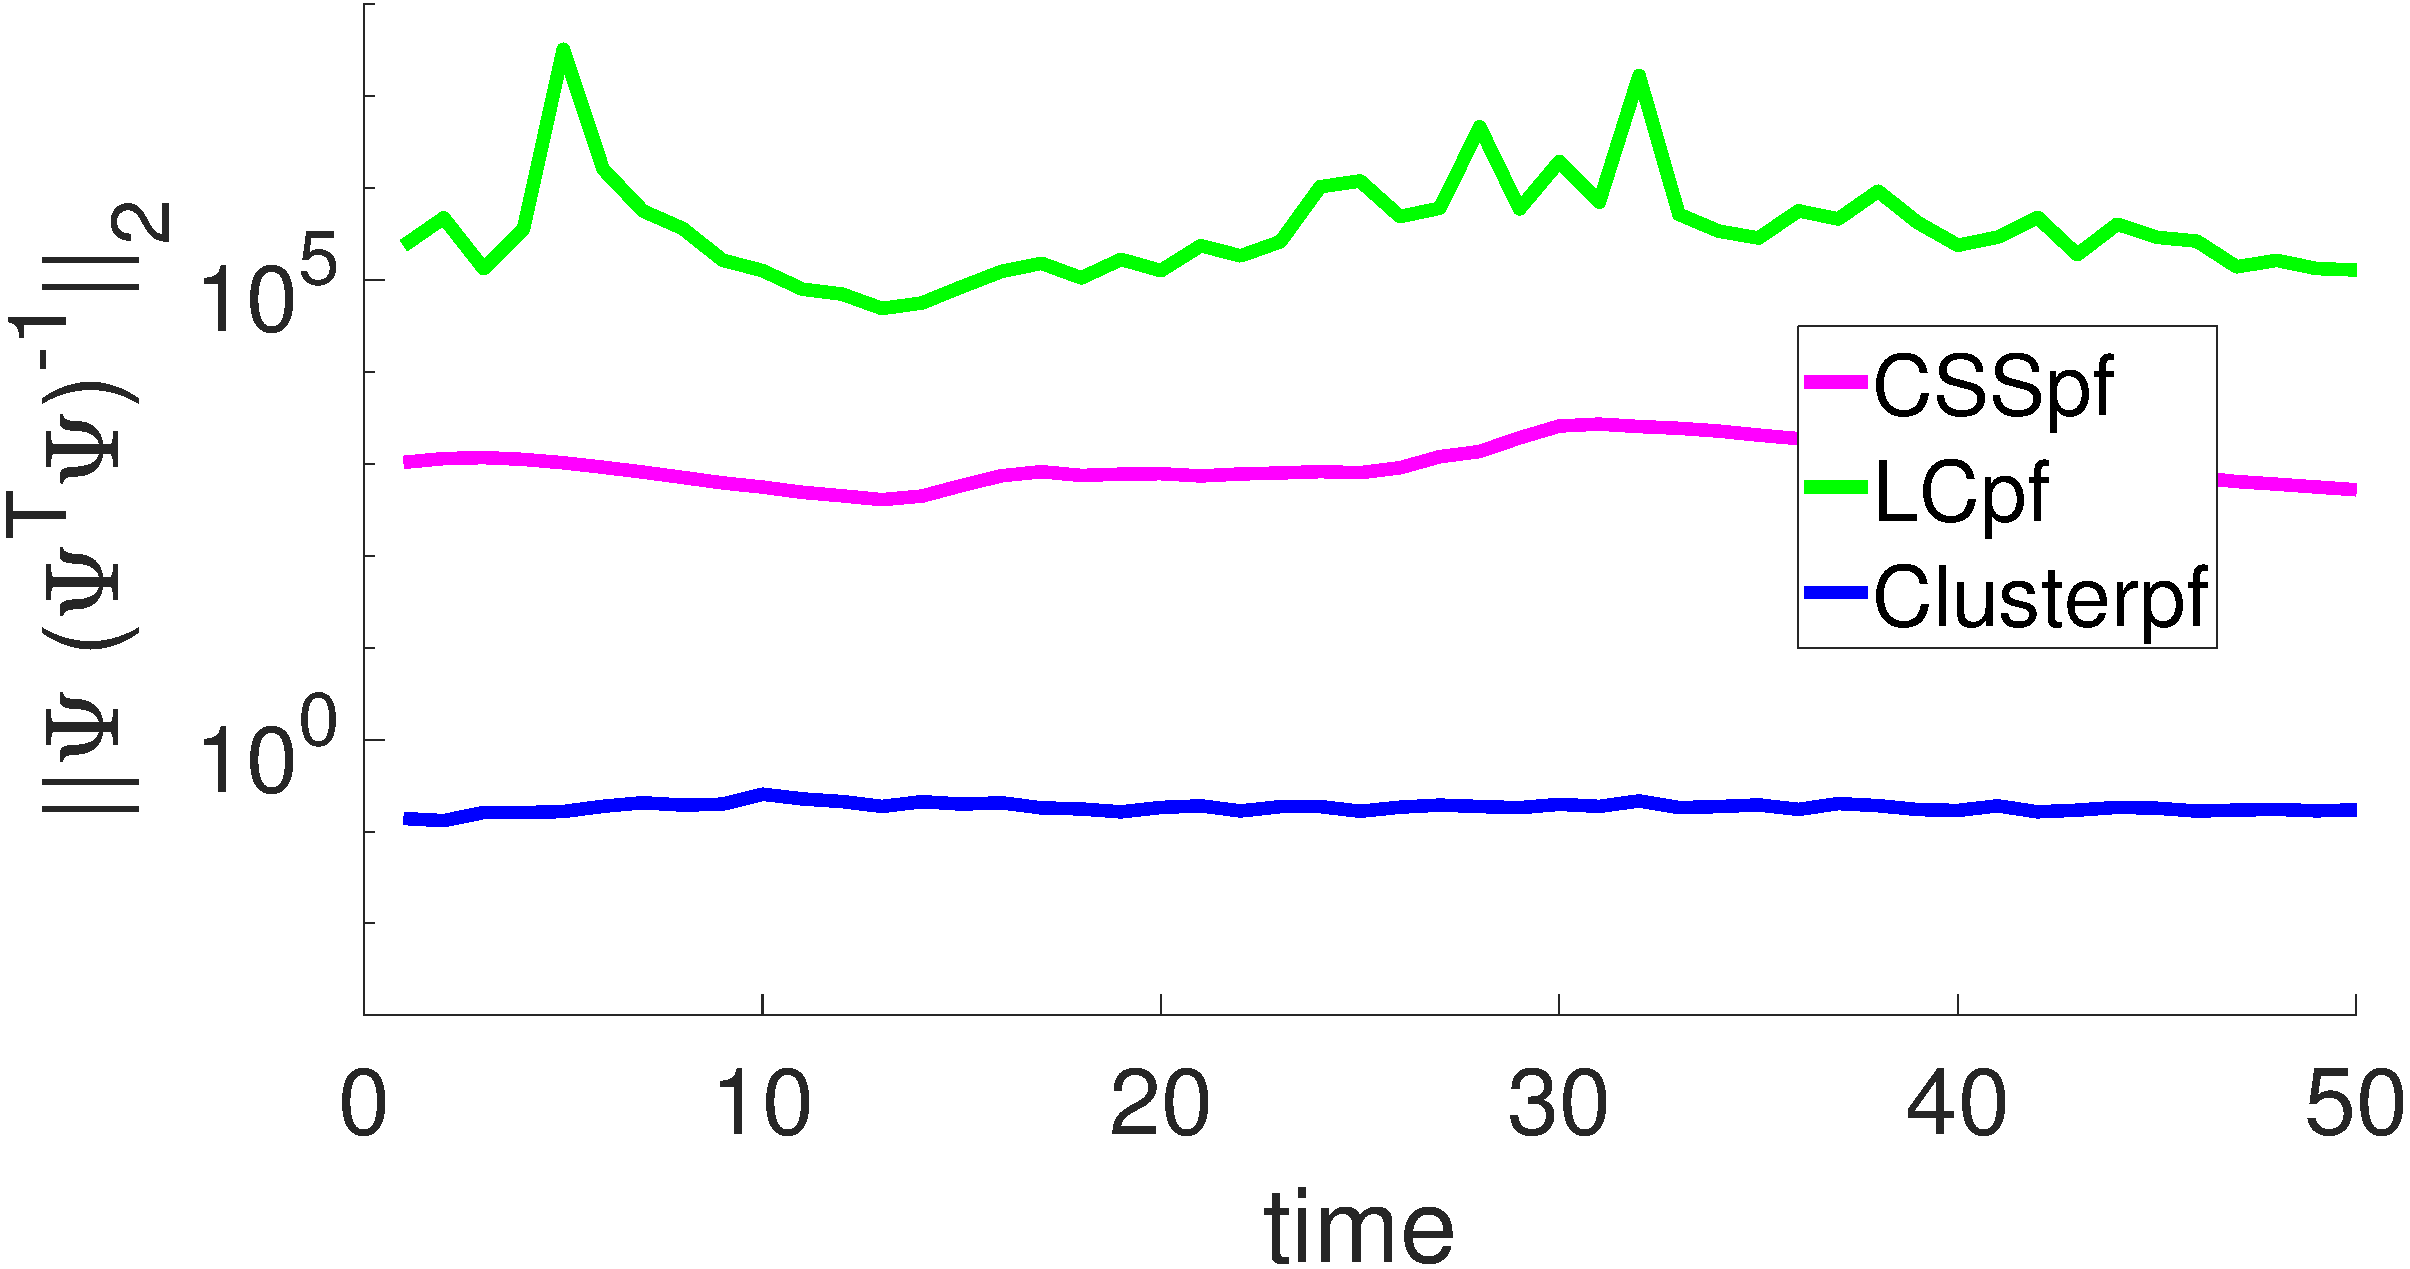
\includegraphics[width=0.49\textwidth]{Figures/Psi_time_track1}}
\end{subfigure}
\begin{subfigure}[Track 2]
{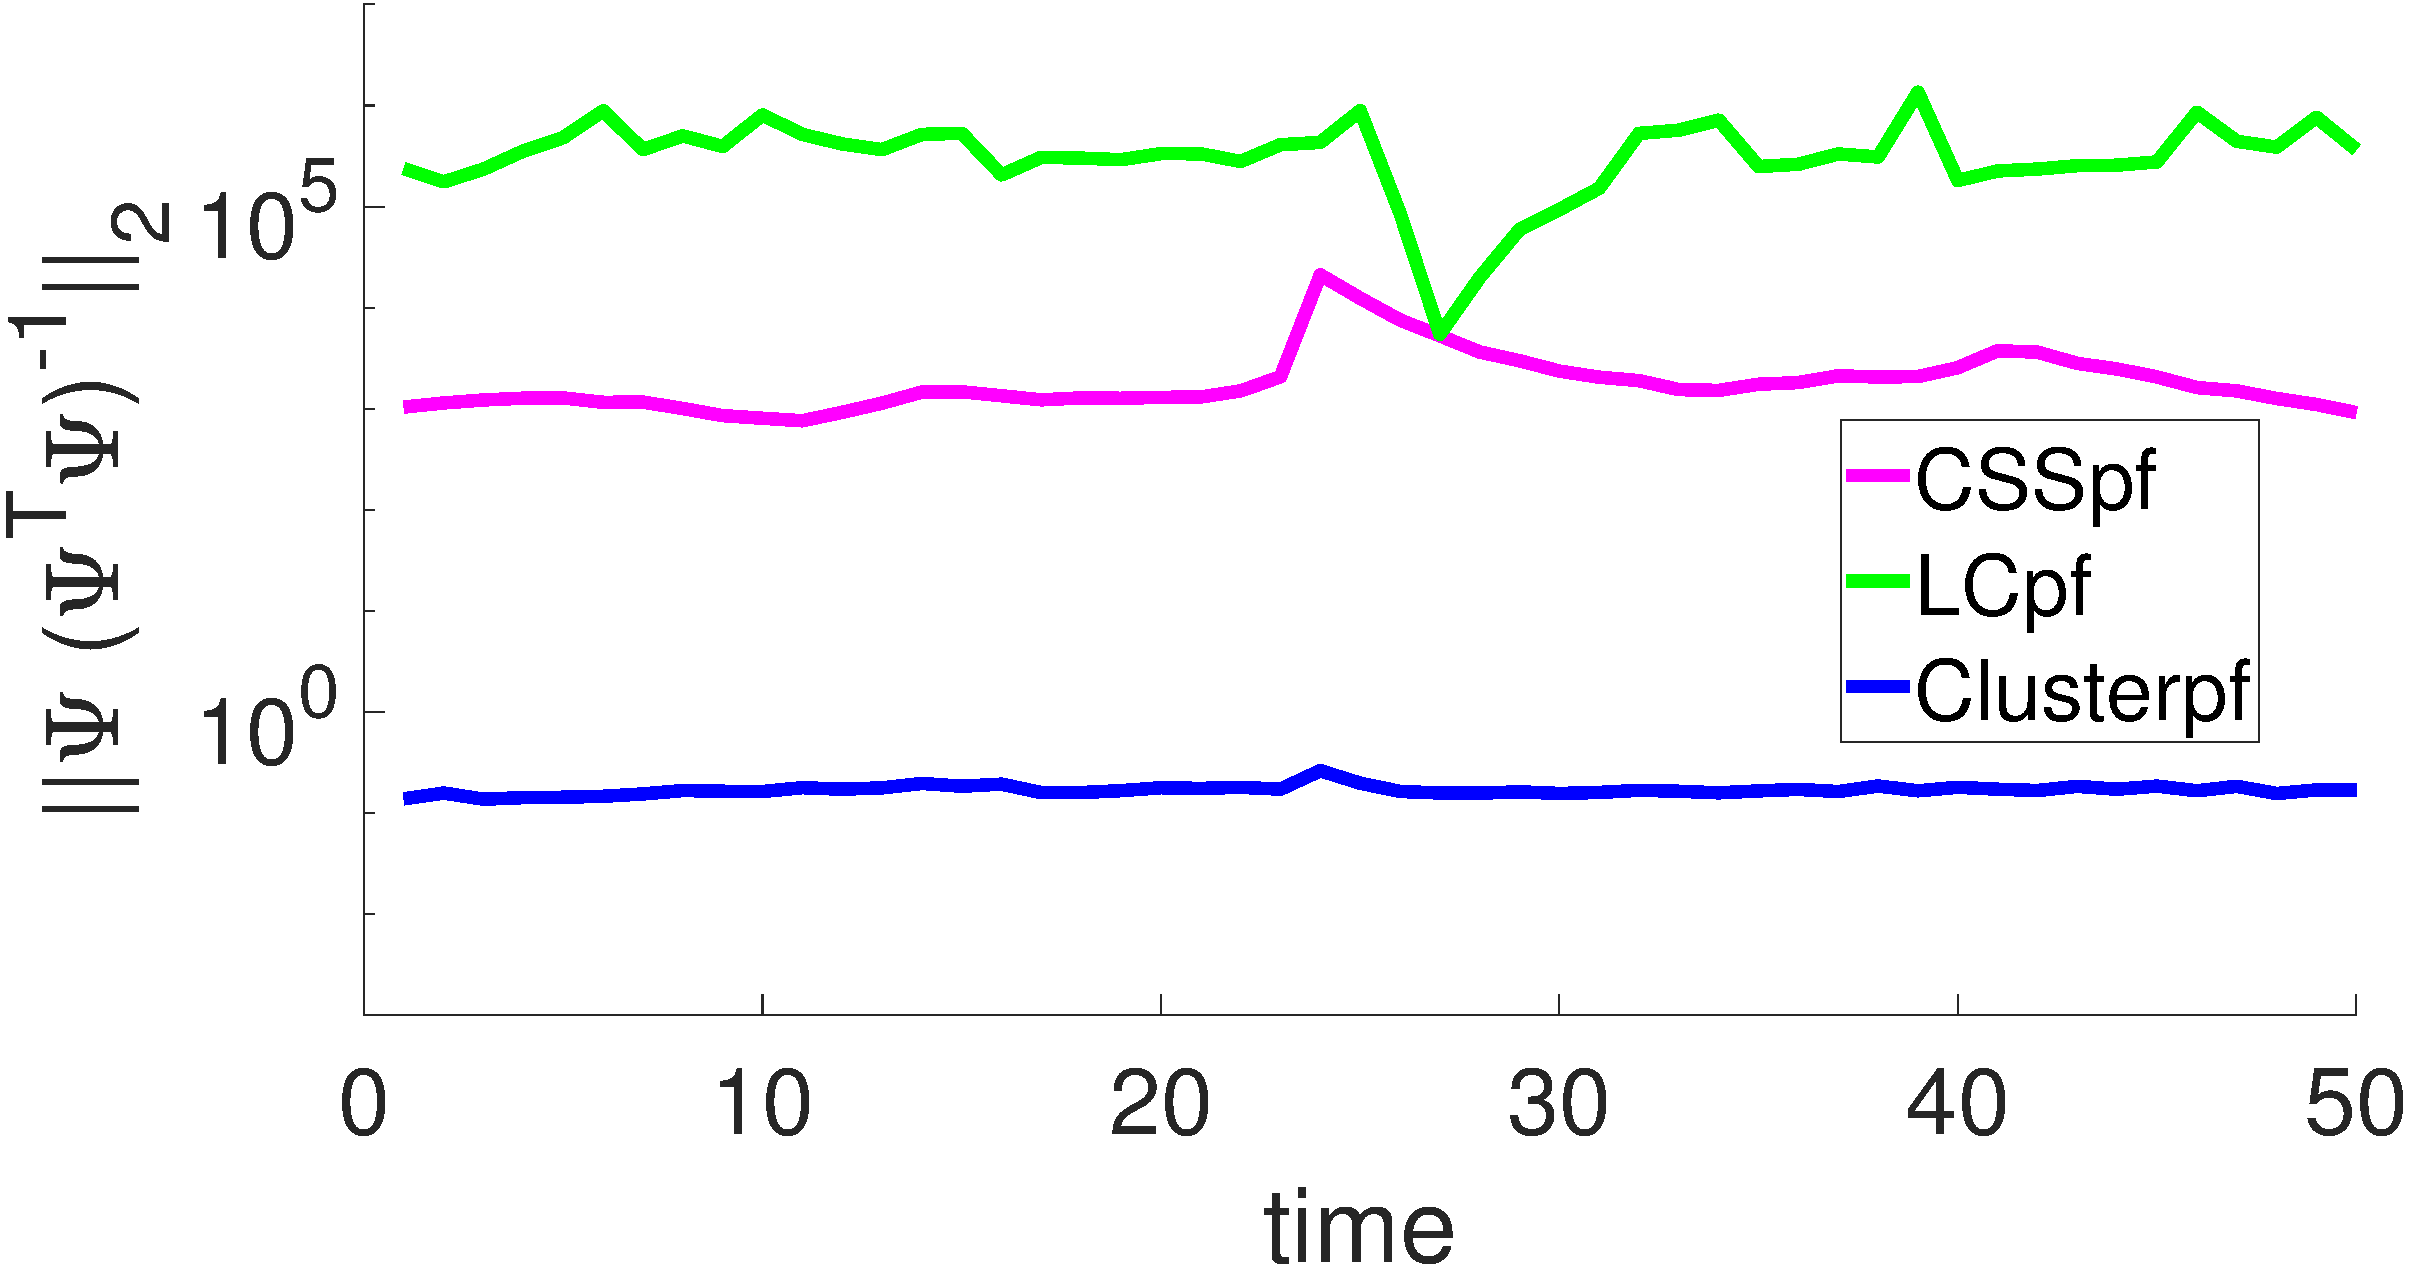
\includegraphics[width=0.49\textwidth]{Figures/Psi_time_track2}}
\end{subfigure}
\begin{subfigure}[Track 3]
{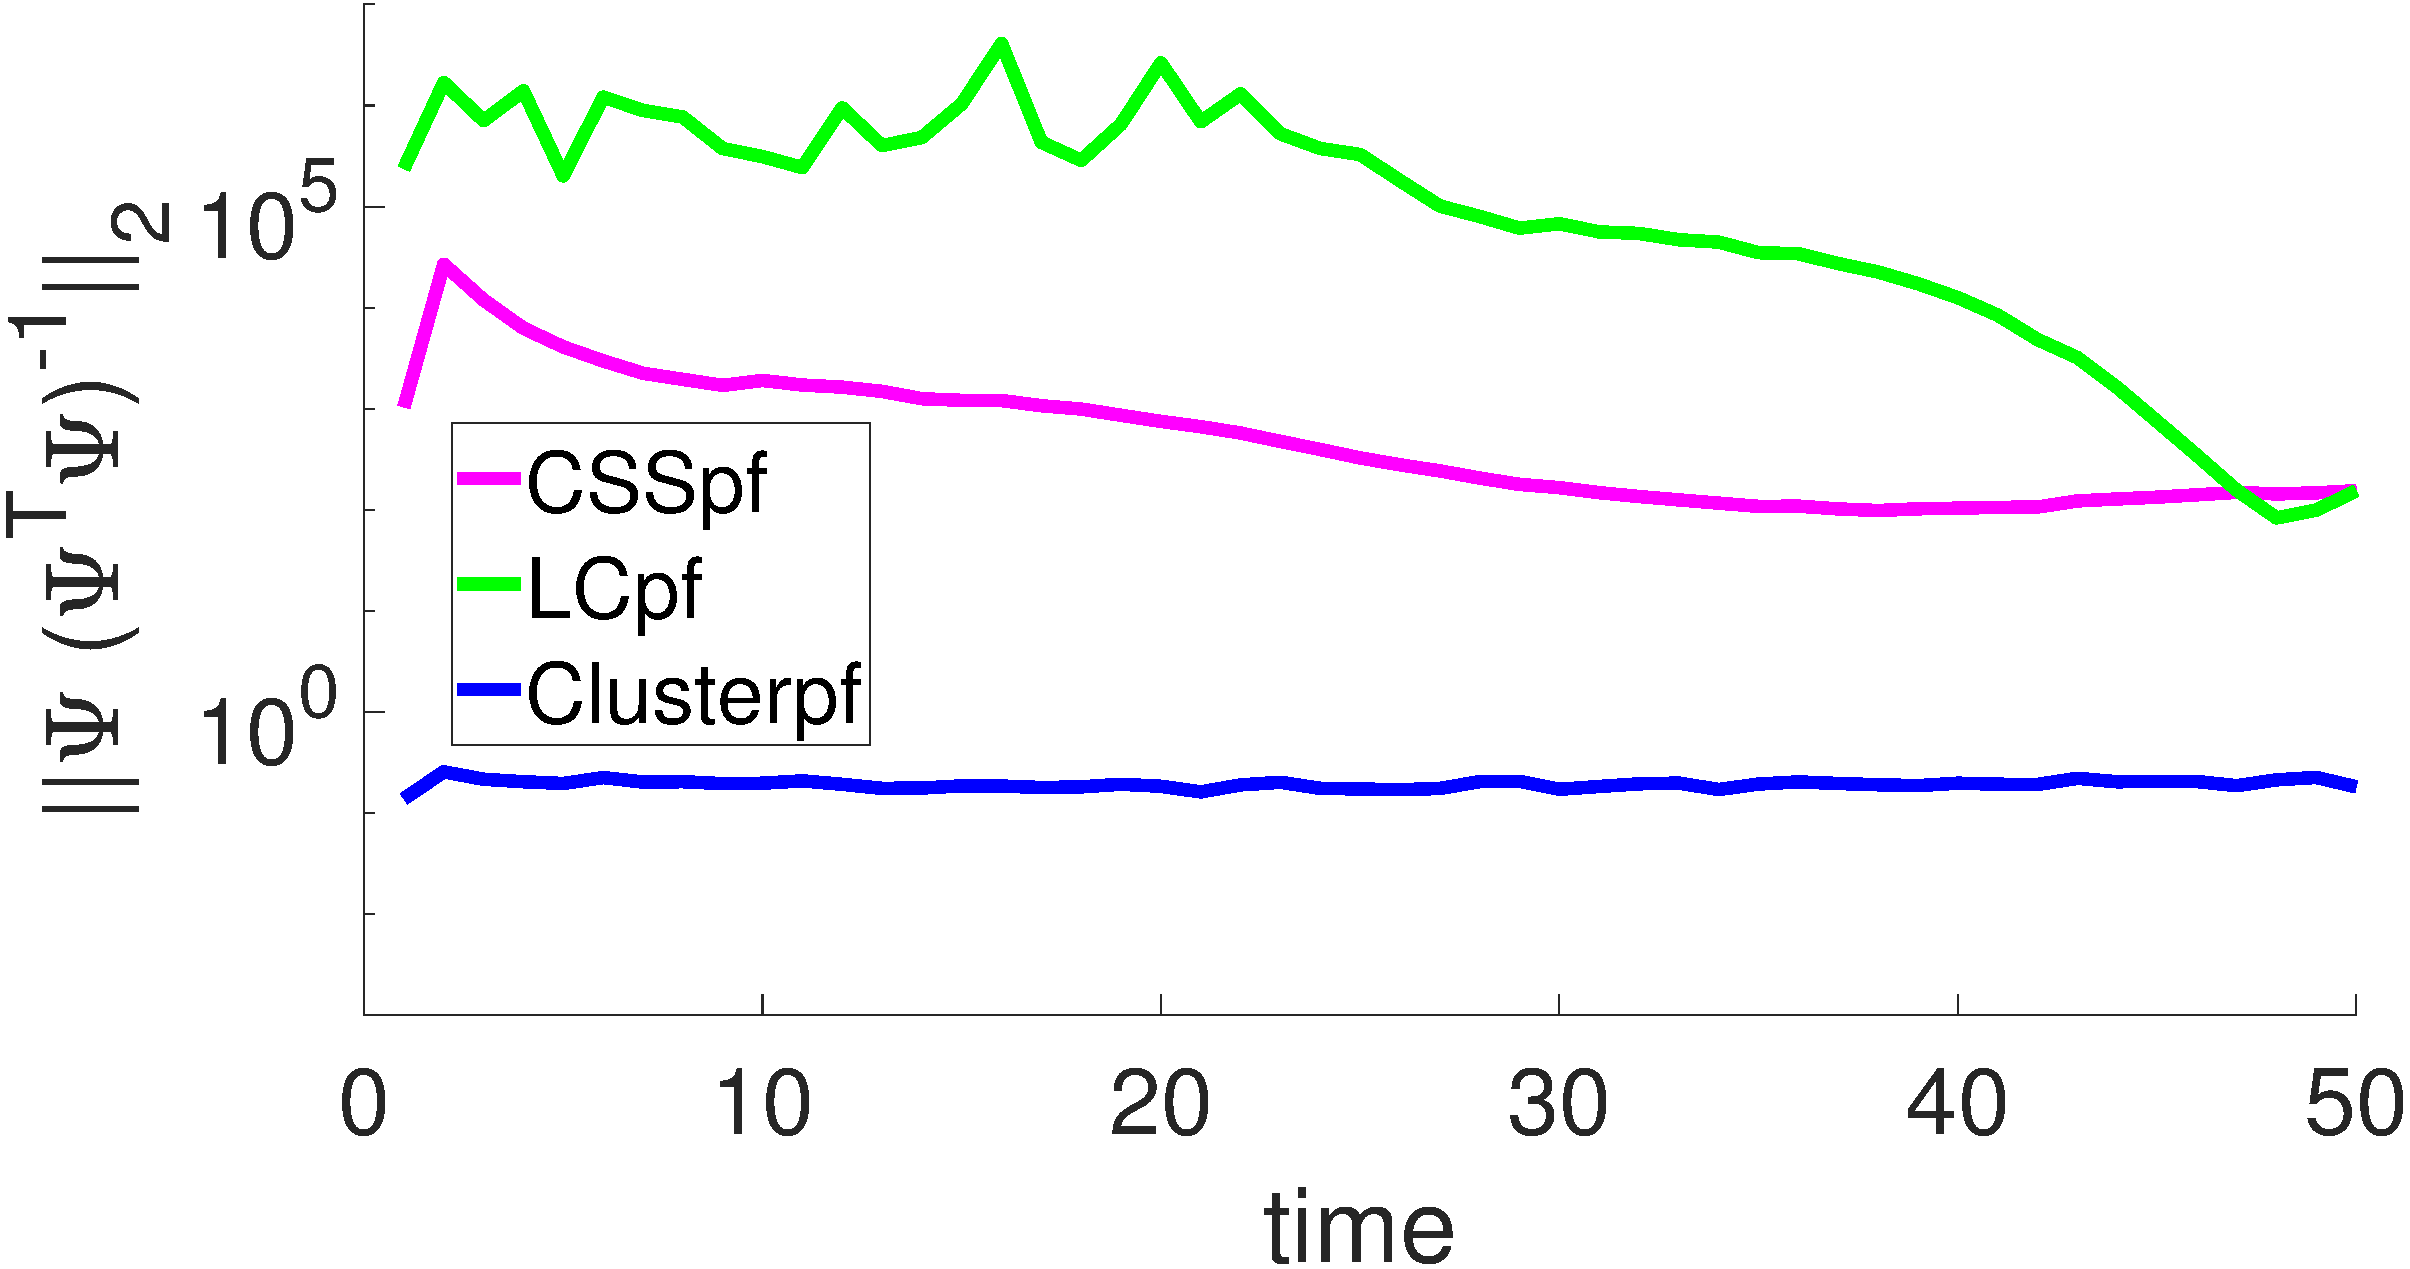
\includegraphics[width=0.49\textwidth]{Figures/Psi_time_track3}}
\end{subfigure}
\caption{Average value of $||\Psi (\Psi^T\Psi)^{-1}||_2$ over time for CSSpf, LCpf and Clusterpf}
\label{fig:Psi_time}
\end{figure}

%In fact, we can take Eq.~\eqref{eqn:gossip_alpha} further and obtain
%\begin{equation}
%\gamma^T = \alpha^T\Psi^T = W^{k+1}
%\underbrace{\left[
%\begin{array}{c}
%\gamma_1^T \\
%... \\
%\gamma_S^T \\
%\end{array}\right]\Psi(\Psi^T\Psi)^{-1}\Psi^T}_{\text{Pseudo log-likelihood}}
%\label{eqn:pseudo_llg}
%\end{equation}

%We obtain the coefficient vector $\alpha'$ by applying a max-consensus algorithm over the network
%\begin{equation}
%\alpha' = \text{MaxConsensus}(\alpha_1(k+1)^T,...\alpha_S(k+1)^T)
%\end{equation}
%
%This max-consensus  

%From the multiplicative property of matrix norm, we have
%\begin{equation}
%\left\vert\left\vert \left[
%\begin{array}{c}
%\gamma_1^T \\
%... \\
%\gamma_S^T \\
%\end{array}\right]\Psi(\Psi^T\Psi)^{-1}\Psi^T\right\vert\right\vert
%\leq 
%\left\vert\left\vert \left[
%\begin{array}{c}
%\gamma_1^T \\
%... \\
%\gamma_S^T \\
%\end{array}\right]\right\vert\right\vert \cdot
%||\Psi||\cdot ||(\Psi^T\Psi)^{-1}||\cdot ||\Psi^T||
%\end{equation}

\section{Bounding the error propagation}
In this section, we seek to bound the error in the presented particle filters. Let $\hat{\gamma}(x_i)$ denote the approximate joint particle log-likelihood for particle $x_i$ and let $\gamma(x_i)$ denote its true joint particle log-likelihood. Our objective is to derive an upper bound for $\frac{||\hat{\gamma}(x_i)-\gamma(x_i)||}{||\gamma(x_i)||}$ for all particles.

All distributed filters presented in this paper follow the same general steps:
\begin{enumerate}
\item Each sensor computes local particle log-likelihoods
\item Each sensor encodes the local log-likelihoods into $m$ coefficients
\item Gossip and max-consensus algorithms are used to compute the $m$ aggregate coefficients. 
\item Approximate joint log-likelihoods are recovered from the aggregate coefficients. 
\end{enumerate}

Therefore, the discrepancy between true log-likelihoods $\gamma(x_i)$ and the final approximate value $\hat{\gamma}(x_i)$ comes from two sources: the encoding error and the gossiping error. The first error is the discrepancy between true log-likelihoods and its reconstructions using $m$ coefficients. The second error occurs when sensors do not obtain the true aggregate coefficient values after a finite number of gossiping iterations. 

Consider the encoding error first. Let $\gamma_m(x_i)$ denote the approximate log-likelihood recovered from $m$ coefficients. More specifically, we have
\begin{align}
\gamma_m^{\text{LC}} &= \Psi^{\text{LC}}\alpha^{\text{LC}} \\
\gamma_m^{\text{LC-GS}} &= \Psi^{\text{LC-GS}}\alpha^{\text{LC-GS}} \\
\gamma_m^{\text{LA}} &= \Psi^{\text{LA}}\alpha^{\text{LA}} \\
\gamma_m^{\text{LC}} &= \Psi^{\text{LC}}\alpha^{\text{LC}} \\
\gamma_m^{\text{Cluster}} &= \arg \min_{\gamma} \gamma^T L \gamma \quad \Psi^{\text{Cluster}}\gamma = \alpha^{\text{LC}} \\
\gamma_m^{\text{CSS}} &= \Psi^{\text{CSS}}\alpha^{\text{CSS}}
\end{align}

Without loss of generality, we define the following bound on encoding error for sensor $s$
\begin{equation}
|\gamma_{m,s}(x_i) - \gamma_s(x_i)|\leq -\delta_m\gamma_s(x_i)
\label{eqn:encoding_error_ss}
\end{equation}

With suitable normalization, we have $\gamma_s(x_i)\leq 0 \quad \forall x_i, s$ so that the right hand of Eq.~\eqref{eqn:encoding_error_ss} is always positive. Then we have
\begin{align}
\left\vert\gamma_{m}(x_i) - \gamma(x_i)\right\vert &=
\left\vert\sum_s \gamma_{m,s}(x_i)-\gamma_s(x_i) \right\vert \nonumber \\
&\leq \sum_s\left\vert \gamma_{m,s}(x_i)-\gamma_s(x_i) \right\vert \nonumber \\
&\leq \delta_m\sum_s -\gamma_s(x_i) \nonumber\\
&= \delta_m \left\vert \sum_s \gamma_s(x_i)\right\vert \nonumber \\
&= \delta_m \left\vert \gamma(x_i)\right\vert
\label{eqn:encoding_error}
\end{align}
where the second equality holds since $-\gamma_s(x_i)\geq 0\quad \forall s$. 

Eq.~\eqref{eqn:encoding_error} gives us an upper bound on the encoding error. The ratio term $\delta_m$ depends on the specific filter and the number of coefficients $m$. We can rewrite Eq.~\eqref{eqn:encoding_error} to yield
\begin{equation}
\gamma_m(x_i) \leq (1+\delta_m)\gamma(x_i)
\end{equation}

Next, we consider the gossiping error. Let $\hat{\alpha}$ denote the coefficients obtained after gossip and max-consensus iterations. This gives us the approximate log-likelihoods $\hat{\gamma} = F(\Psi, \hat{\alpha})$. 

Again, without loss of generality, we define the following bound
\begin{equation}
\frac{|\gamma_m(x_i)-\hat{\gamma}(x_i)|}{|\gamma_m(x_i)|} \leq \delta_{Gossip}
\label{eqn:gossiping_error}
\end{equation}

Consider LApf, LCpf, LCpf-GS and CSSpf. Let $\Psi_i$ denote the $i^{th}$ row of encoding matrix $\Psi$, we can derive an upper bound for the gossiping error as follows:
\begin{align}
\frac{||\gamma_m(x_i)-\hat{\gamma}(x_i)||}{||\gamma_m(x_i)||}&=\frac{||\Psi_i\alpha-\Psi_i\hat{\alpha}||}{||\Psi_i\alpha||} \\
&\leq ||\Psi_i^T||\frac{||\Psi_i\alpha-\Psi_i\hat{\alpha}||}{||\Psi_i^T\Psi_i\alpha||} \\
&\leq ||\Psi_i^T|| \cdot ||\Psi_i||\cdot \frac{||\alpha-\hat{\alpha}||}{||\Psi_i^T\Psi_i\alpha||} 
\end{align}
where the first inequality follows from $||\Psi_i^T\Psi_i \alpha|| \leq ||\Psi_i^T||\cdot ||\Psi_i\alpha||$.

Depending on the encoding matrix $\Psi$, the upper bound an be quite loose. We follow the same approach and derive a lower bound which may be more useful. 

\begin{align}
\frac{||\gamma_m(x_i)-\hat{\gamma}(x_i)||}{||\gamma_m(x_i)||}&=\frac{||\Psi_i\alpha-\Psi_i\hat{\alpha}||}{||\Psi_i\alpha||} \nonumber \\
&\geq \frac{||\Psi_i^T\Psi_i\alpha-\Psi_i^T\Psi_i\hat{\alpha}||}{||\Psi_i^T||\cdot ||\Psi_i\alpha||}
\end{align}

Putting everything together, we obtain
\begin{align}
\frac{|\hat{\gamma}(x_i) - \gamma(x_i)|}{|\gamma(x_i)|}&=\frac{|\hat{\gamma}(x_i) -\gamma_m(x_i) + \gamma_m(x_i) - \gamma(x_i)|}{|\gamma(x_i)|} \\
&\leq \frac{|\hat{\gamma}(x_i) -\gamma_m(x_i)|}{|\gamma(x_i)|}+\frac{|\gamma_m(x_i) - \gamma(x_i)|}{|\gamma(x_i)|} \\
&\leq (1+\delta_m)\frac{|\hat{\gamma}(x_i) -\gamma_m(x_i)|}{|\gamma_m(x_i)|}+\frac{|\gamma_m(x_i) - \gamma(x_i)|}{|\gamma(x_i)|} \\
&\leq (1+\delta_m)\delta_{gossip} + \delta_m  = \delta
\label{eqn:error_bound}
\end{align}

Consider Eq.~\eqref{eqn:error_bound}. When both the encoding and gossiping errors are present, they have a cascading effect on the overall error propagation. The error is bounded (i.e., less than unity) when both terms are bounded. 

To validate the derived error bounds, we run the following simulations. We run a centralized BSpf to track the target. At each time step, we also compute the particle weights using the four distributed filters. we also compute and report the following the metric:
\begin{enumerate}
\item $\max_{s,x_i} \frac{|\gamma_{m,s}(x_i)-\gamma_s(x_i)|}{|\gamma_s(x_i)|}$: estimate of $\delta_m$
\item $\max_{x_i} \frac{|\gamma_m(x_i)-\hat{\gamma}(x_i)|}{|\gamma_m(x_i)|}$: estimate of $\delta_{gossip}$ 
\item $||\Psi_i^T|| \cdot ||\Psi_i||\cdot \frac{||\alpha-\hat{\alpha}||}{||\Psi_i^T\Psi_i\alpha||}$: upper limit of $\delta_{gossip}$ for LApf, LCpf, LCpf-GS and CSSpf
\item $\frac{||\Psi_i^T\Psi_i\alpha-\Psi_i^T\Psi_i\hat{\alpha}||}{||\Psi_i^T||\cdot ||\Psi_i\alpha||}$: lower limit of $\delta_{gossip}$ for LApf, LCpf, LCpf-GS and CSSpf
\item $\max_{x_i} \frac{|\hat{\gamma}(x_i) - \gamma(x_i)|}{|\gamma(x_i)|}$: discrepancy in log-likelihood
\item $(1+\delta_m)\delta_{gossip} + \delta_m$: estimate of $\delta$
\end{enumerate}


\section{Conclusion}
\label{sec:conclusion}
In this report, we present four distributed particle filters for single-target bearing-only tracking. CSSpf approximates the log-likelihood function using six sufficient statistics. LCpf uses likelihood consensus to encode the particle log-likelihoods. LApf constructs a graph over all particles and uses the eigenvectors of resulting Laplacian matrix to encode the particle log-likelihood. Finally, Clusterpf groups particles into clusters, computes the cluster joint log-likelihood and recovers individual particle weights using convex minimization. 

We study each individual algorithm's performance and compare them against each other. LCpf is very fast, but is highly susceptible to gossiping error and requires a much higher communication overhead to achieve adequate tracking performance. The LApf and Clusterpf yield robust tracking performance in all tested scenarios; but they also have the highest runtime by a large margin. More interestingly, when minimal communication overhead is permitted, LApf and Clusterpf are still able to yield robust performance while the other filters would break down. These results make LApf and Clusterpf extremely attractive in energy-constrained tracking scenarios. 

\bibliographystyle{IEEEtran}
\bibliography{Refs}

\end{document}
